\documentclass[12pt, twoside]{report} %Tamaño de letra 12, tipo report y hago que sea a doble pagina, queda bonito
%si se imprime como libro a 2 lados, 
\usepackage[utf8]{inputenc} %UTF8 para caracteres 
\usepackage{graphicx}       %Paquete para insertar imágenes
\graphicspath{{images/}}  %Directorio de las imágenes 
\usepackage[a4paper, width=145mm, top=25mm, bottom=25mm, bindingoffset=6mm]{geometry}
%Tamaño del papel a4, anchura del texto 145mm , margenes top, bottom de 25mm
%offset para que no sea tan marcado el hecho de que los margenes están disparejos para que en modo doble lado se vea
%bonito
%\usepackage[spanish, mexico]{babel} %Idioma español de lo autogenerado
\usepackage{fancyhdr}%Agrega headers y footers


\setlength{\headheight}{15.09pt}

\title{
    {Análisis y procesamiento de metadatos geográficos para su 
    uso y explotación}\\
    {\large Facultad de Ciencias, UNAM}\\
    {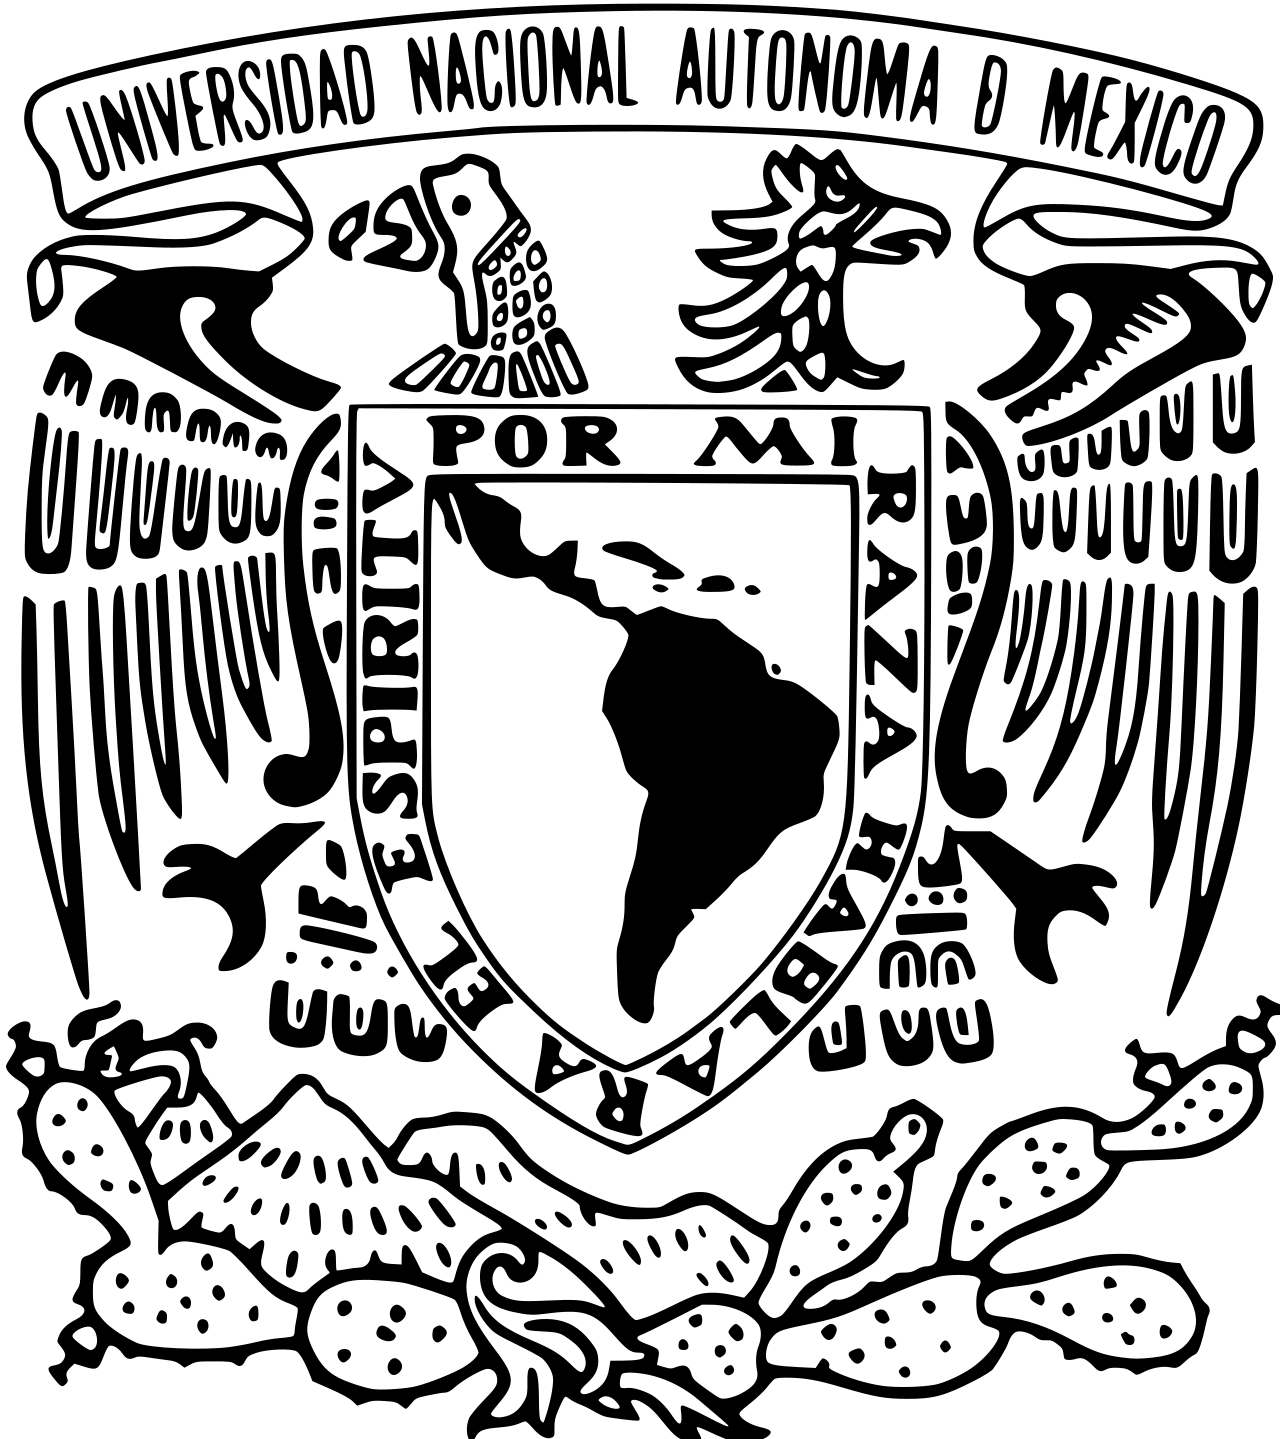
\includegraphics[scale=0.15]{portada/escudo.png}}
}
\author{Alejandro Iabin Arteaga Hernández}

\pagestyle{fancy}
\fancyhf{}
\fancyhead[LE,RO]{Overleaf}
\fancyhead[RE,LO]{Guides and tutorials}
\fancyfoot[CE,CO]{\rightmark}
\fancyfoot[LE,RO]{\thepage}
\renewcommand{\headrulewidth}{2pt}
\renewcommand{\footrulewidth}{1pt}

\begin{document}

    \maketitle

        \tableofcontents


    \chapter*{Síntesis}
    Lorem ipsum dolor sit amet, consectetur adipiscing elit. Proin non nisl eget nulla condimentum fringilla aliquet quis ante. Praesent at elit ac magna tincidunt posuere. Aenean id felis id diam bibendum consequat eget mollis orci. Orci varius natoque penatibus et magnis dis parturient montes, nascetur ridiculus mus. Donec eu velit dapibus nisl tincidunt sollicitudin ut sit amet nisi. Nam vel nulla ut odio malesuada aliquet sit amet in lectus. Donec ipsum nisi, dapibus a bibendum ut, venenatis sit amet elit. Duis lectus nisi, eleifend ac aliquam eu, mollis vitae velit. Aliquam maximus auctor ex sit amet malesuada. Nam in fringilla velit. Cras pharetra purus ut turpis pretium, vel eleifend odio tristique. Morbi at tellus id elit iaculis laoreet. Aliquam pellentesque leo ullamcorper porta dapibus. Aenean at posuere nisl. Cras eget nisi vel elit accumsan egestas. Aenean porttitor dolor at erat congue feugiat.

Vestibulum vitae condimentum mauris. Suspendisse vulputate lacinia dolor, in lobortis quam vestibulum sit amet. Duis porta neque at lorem venenatis, sit amet luctus turpis venenatis. Nullam dapibus volutpat erat sit amet finibus. Donec nulla risus, semper at libero at, scelerisque laoreet risus. Suspendisse potenti. Ut et lectus pharetra, pretium justo vitae, pharetra justo. Nulla blandit vestibulum ex, at efficitur nisl tincidunt ac. Vestibulum venenatis, ante at venenatis maximus, orci magna volutpat sapien, nec fringilla felis elit auctor mi.

Aenean eget accumsan neque. Donec volutpat nunc a nunc vestibulum fermentum. Aenean velit purus, lacinia eget lacus quis, cursus tincidunt dui. Aliquam euismod tempus pretium. Maecenas posuere sit amet arcu nec facilisis. Mauris id nibh varius, lacinia turpis in, sodales nunc. Cras ex turpis, sagittis sit amet vestibulum in, dignissim id ipsum. Donec mattis, nunc vitae accumsan rutrum, ligula sapien mollis elit, a dignissim sem metus in nulla. In hac habitasse platea dictumst. Nam orci nisi, lacinia vitae egestas ut, maximus non sem. Integer vehicula elementum felis non vulputate. Sed pellentesque arcu quam, quis dignissim lectus auctor vulputate. Morbi interdum risus justo, at tincidunt justo faucibus ut. Nulla et turpis in ante dictum aliquam.

Integer feugiat sollicitudin condimentum. Vestibulum posuere id nibh dignissim feugiat. Donec vitae massa nec nisl faucibus placerat sit amet quis mi. Vestibulum dui elit, elementum scelerisque aliquet ut, ultrices id neque. Donec vestibulum sollicitudin justo in volutpat. Proin malesuada gravida massa non tempor. Suspendisse malesuada rhoncus arcu eu efficitur. Maecenas id accumsan leo. Aliquam eu gravida diam. Vestibulum euismod dui eros, id fermentum ex tempor in. Nulla facilisi. Morbi elementum sed elit vitae tincidunt. Ut magna felis, posuere ut vulputate at, lacinia at est. Pellentesque ac efficitur neque.

Cras vel placerat dui, vitae pellentesque neque. Vestibulum at lacus dui. Donec pellentesque nunc eu lectus condimentum, nec lobortis tellus euismod. Nam laoreet commodo purus et tempus. Ut suscipit diam turpis, non pulvinar massa maximus et. Mauris aliquet vestibulum risus, non tristique nibh mattis sed. Mauris et tristique nunc. Nam sit amet orci in ipsum porta congue. In sodales felis ut risus pharetra venenatis. Maecenas eget felis eleifend, rutrum lorem id, tempus tortor. Mauris iaculis suscipit feugiat. Pellentesque a leo ut diam finibus ultricies. Maecenas enim velit, finibus et aliquam vitae, iaculis sit amet magna. Aenean eget orci a mi vehicula efficitur non rhoncus orci. Fusce non tempus metus.

Nam at feugiat metus, id efficitur diam. Donec massa leo, ornare nec gravida in, elementum eget nisl. Sed at lorem suscipit, facilisis sapien sed, euismod mi. Fusce libero nisl, lobortis vitae neque id, pretium finibus eros. Quisque pharetra elit urna, at mattis justo pellentesque a. Orci varius natoque penatibus et magnis dis parturient montes, nascetur ridiculus mus. Quisque at massa dignissim, eleifend erat nec, mattis purus.

Phasellus leo diam, porttitor vitae molestie sit amet, vehicula vel enim. Nullam id porta lectus, vel commodo tortor. Ut at est iaculis, venenatis mi ac, consequat magna. Pellentesque quis magna eget ipsum feugiat congue. Proin nec mauris magna. Aliquam viverra dui vitae semper ultrices. Duis vitae est tortor. Maecenas hendrerit nunc eget ipsum rhoncus efficitur. Aenean eget tortor lectus.

Cras id velit eleifend, suscipit ante vel, interdum enim. Etiam maximus mauris sed ultrices feugiat. Morbi condimentum a nibh ut sodales. Donec ex nunc, rutrum quis bibendum at, efficitur nec turpis. Duis magna mauris, scelerisque id tellus quis, tincidunt maximus libero. Vivamus vehicula tellus eu vulputate pretium. Praesent mollis, elit vel congue feugiat, lectus odio feugiat tellus, et scelerisque augue urna quis lectus. Morbi sem sem, varius et velit at, laoreet dignissim felis. Curabitur luctus varius ultricies. In vel dolor diam. Nulla nulla ligula, pharetra et semper sed, facilisis vestibulum risus. Praesent molestie massa sit amet pharetra pulvinar.

Ut feugiat pharetra imperdiet. Mauris fermentum aliquet magna, ut venenatis leo rutrum a. Integer rutrum velit risus. Ut volutpat massa id enim sodales, a congue urna aliquet. Nulla imperdiet, nisi eu eleifend tincidunt, eros ex blandit sapien, sed bibendum arcu purus id tellus. Curabitur at ipsum imperdiet, cursus libero eget, interdum neque. Phasellus odio erat, iaculis quis nulla quis, vehicula varius nunc. Etiam quis suscipit leo, at molestie elit. Maecenas condimentum turpis non sapien vehicula semper. Quisque justo ipsum, cursus ut bibendum sit amet, laoreet in magna.

Sed rutrum sapien ligula, a malesuada turpis euismod nec. Orci varius natoque penatibus et magnis dis parturient montes, nascetur ridiculus mus. Integer et arcu eu nisi iaculis luctus. Fusce a volutpat ante, venenatis convallis eros. In nec sollicitudin orci. Morbi suscipit libero vitae neque convallis, vitae ornare dui interdum. Mauris eleifend non sapien eu iaculis. Proin mattis ut dui sed pharetra.

Nam mollis convallis ligula sed semper. Lorem ipsum dolor sit amet, consectetur adipiscing elit. Aenean commodo vehicula velit ac placerat. Vivamus tincidunt neque tortor, in vulputate est lacinia et. Suspendisse et libero in nulla pulvinar maximus a non sapien. Proin eleifend sem ut quam pulvinar, et ultricies eros porta. Vivamus vestibulum eleifend dui quis facilisis. In commodo, turpis in semper porta, elit odio tincidunt elit, ut egestas metus est lacinia augue. Sed interdum arcu at nunc scelerisque porttitor. Fusce ac neque vehicula justo pretium semper.

Mauris venenatis finibus lacinia. Curabitur a efficitur enim. Phasellus nunc leo, venenatis ut quam eget, sollicitudin consectetur felis. Donec feugiat lacus sed mi condimentum, nec venenatis dolor sagittis. Duis et consectetur neque. Interdum et malesuada fames ac ante ipsum primis in faucibus. Aenean porta scelerisque magna, eget consequat elit iaculis eget. Aliquam pellentesque a eros et luctus. In consequat ligula sed ligula lobortis blandit. Cras dignissim nisl et eros interdum, sed luctus nulla sodales. Quisque eget orci dolor. Sed sodales pharetra lorem eget ultricies. Nam sit amet libero quis nibh tempus viverra sed eu eros. Phasellus ultrices nec arcu ac mollis. Nam a quam ac leo cursus faucibus.

Sed ut faucibus ex, sodales pretium massa. Interdum et malesuada fames ac ante ipsum primis in faucibus. Sed nisl ligula, egestas id nunc eget, suscipit posuere dui. Curabitur non velit neque. Suspendisse ultricies, sapien vitae porttitor gravida, metus nibh commodo orci, in varius augue quam imperdiet lorem. Ut vitae dolor elementum, laoreet ante ac, suscipit quam. Orci varius natoque penatibus et magnis dis parturient montes, nascetur ridiculus mus.

Suspendisse vehicula eget turpis nec condimentum. Praesent convallis porttitor metus at congue. Aenean id magna ut nisi scelerisque dignissim. Cras at orci sed quam molestie dictum nec vitae est. Fusce maximus, erat eu pulvinar iaculis, dui arcu vulputate mi, eu sagittis magna purus eu risus. Mauris id vehicula dolor, vitae dictum nulla. Cras a velit id ipsum fringilla sodales. Donec luctus, ante non sagittis dictum, libero urna feugiat nulla, tincidunt cursus risus libero vitae ligula.

Suspendisse consequat justo risus, sit amet cursus risus molestie ut. Etiam aliquet lectus vitae nisl semper, eu viverra felis laoreet. Phasellus sed orci ut nunc interdum sodales. Nulla ut arcu sed enim imperdiet congue. Nunc quis commodo ex. Etiam semper mauris diam, eget condimentum dolor suscipit tristique. Suspendisse arcu nulla, rutrum elementum arcu eget, malesuada euismod dui. Sed pellentesque malesuada nunc nec maximus. Phasellus et fermentum magna, at malesuada nisl. Aliquam erat volutpat. Curabitur sed nunc euismod, tincidunt augue a, volutpat dui. Mauris commodo felis viverra, feugiat erat ut, sollicitudin arcu. Nam tincidunt lorem libero, a lobortis nisl condimentum a. Nulla eu nisi fermentum, ornare ante eget, laoreet erat. Ut tincidunt tortor in justo dictum auctor. Praesent id ornare dui.

Aliquam fermentum molestie eros. Orci varius natoque penatibus et magnis dis parturient montes, nascetur ridiculus mus. Vestibulum aliquet sed odio non pretium. Nulla felis arcu, vehicula nec libero nec, rutrum sagittis magna. Curabitur metus mauris, vestibulum eu nunc ut, semper pellentesque orci. Maecenas in varius erat, gravida sodales nulla. Class aptent taciti sociosqu ad litora torquent per conubia nostra, per inceptos himenaeos. Suspendisse potenti. Nullam eros quam, tempus ac turpis et, accumsan feugiat sem. Suspendisse viverra arcu in laoreet venenatis. Sed sagittis eros et libero aliquet luctus. Vivamus mi purus, pretium dapibus arcu ac, scelerisque porttitor massa. Cras posuere ligula eu turpis ultrices vulputate.

Nam interdum nunc sed mi pharetra, sed aliquam purus gravida. Sed vel purus enim. Nullam leo justo, rhoncus non dui id, pulvinar blandit quam. Proin nisl ex, finibus quis mauris non, lobortis finibus quam. Aenean et justo vitae libero tristique venenatis at eu tellus. Aenean sit amet nisi nibh. Sed eget iaculis lorem. Nam facilisis elementum pellentesque. Maecenas ac sapien ante. Vestibulum dapibus congue pharetra. Nam mi lacus, lacinia non ipsum ut, semper dictum nisi. Donec in eros pretium, pellentesque urna sagittis, sagittis libero. Vivamus sed dui quis arcu porta fringilla. Quisque eu nisl vel nisi vestibulum ultrices. Integer in mi ut eros eleifend porta id vestibulum risus. Sed risus erat, dignissim in nulla eget, convallis vehicula eros.

Aenean sollicitudin sollicitudin ex eu gravida. Phasellus consectetur elit a condimentum laoreet. Curabitur ultrices finibus lectus eget venenatis. In eget suscipit justo. Curabitur vitae diam blandit, imperdiet arcu in, eleifend odio. Lorem ipsum dolor sit amet, consectetur adipiscing elit. Etiam metus neque, sollicitudin sit amet eros eget, rutrum iaculis turpis. Pellentesque semper nisl non leo lacinia, non efficitur quam eleifend. Fusce rutrum ullamcorper dui, eget dictum arcu dictum dignissim. Mauris malesuada mauris in elementum hendrerit. Lorem ipsum dolor sit amet, consectetur adipiscing elit.

Vestibulum ultricies ante vulputate, ultrices tortor ut, blandit mauris. Donec urna massa, gravida a mollis vel, ornare in sapien. Nunc suscipit velit ipsum, nec posuere magna consectetur at. Nullam suscipit mattis urna. Mauris id sagittis nulla, in semper erat. Integer vulputate urna metus, quis lobortis diam sagittis eget. Sed bibendum in augue ac rutrum.

Vivamus finibus posuere urna at aliquam. Nulla at ultrices arcu. Fusce euismod luctus magna id pretium. Etiam tellus enim, sollicitudin non sapien nec, auctor vestibulum leo. Pellentesque mollis tempus lorem a congue. Nunc eu risus egestas, interdum nisl non, sagittis metus. Sed mollis posuere nibh eget accumsan. Mauris scelerisque lacinia lorem.

Nulla eu quam quis erat scelerisque accumsan. Nam rhoncus tristique erat sed fermentum. Duis ipsum nisi, varius sed massa in, interdum posuere massa. Sed quis ex ac velit auctor scelerisque. Phasellus quis fermentum urna. In interdum dolor sed pretium blandit. Proin iaculis commodo placerat. Pellentesque tortor est, mattis eu lorem vel, commodo pellentesque quam. Nunc aliquam tellus eget nulla pellentesque, mollis elementum ante dictum. Phasellus blandit lorem sit amet magna efficitur porttitor. Aenean sagittis malesuada eros. Quisque pharetra euismod pharetra. Nunc tellus justo, feugiat eget lectus a, malesuada vestibulum mi. Maecenas sodales sem augue, vitae efficitur orci malesuada ac. Praesent feugiat magna a auctor convallis.

Donec at ante ac sapien ultricies ultricies quis eu magna. Pellentesque venenatis ante at nibh placerat tincidunt. Sed imperdiet lorem et neque placerat dapibus. Quisque maximus varius tincidunt. Pellentesque pulvinar pharetra ante eget malesuada. Integer blandit nunc cursus enim ornare, in viverra nulla semper. Vestibulum feugiat, risus ultrices iaculis rutrum, massa enim efficitur est, sed pellentesque eros enim condimentum libero. Nam in egestas nulla, vel dignissim leo. Sed sit amet vestibulum ex, ac viverra ipsum. Integer vel nunc id metus rhoncus congue eget sed nunc. Nulla ac libero sed diam sollicitudin sollicitudin lobortis quis lacus.

Etiam elementum scelerisque tempus. Mauris nec enim sapien. Nulla tempor ullamcorper nunc. Fusce et porttitor dolor. Cras aliquam commodo nunc, sit amet vehicula massa venenatis non. Aliquam eget pellentesque dui, at sodales libero. Donec vestibulum eget turpis ac volutpat. Nulla facilisi. Phasellus porta ornare justo, vel ultrices odio sodales et.

Etiam commodo diam at mauris consectetur, non rutrum enim sagittis. Praesent ut velit placerat, iaculis libero et, commodo dolor. Fusce faucibus semper pellentesque. Nullam ac malesuada leo, condimentum fermentum eros. Curabitur vitae leo erat. Class aptent taciti sociosqu ad litora torquent per conubia nostra, per inceptos himenaeos. Aenean ornare rutrum posuere. Aenean semper lacinia massa ut convallis. Class aptent taciti sociosqu ad litora torquent per conubia nostra, per inceptos himenaeos. Sed vulputate leo id dolor efficitur, sed aliquet nunc auctor. Vestibulum fermentum leo ac dignissim dictum. Proin convallis arcu et libero condimentum dapibus.

Nam vitae purus neque. Nam mollis a orci sit amet tristique. Suspendisse id nulla ante. Integer sed tempor sem. Pellentesque habitant morbi tristique senectus et netus et malesuada fames ac turpis egestas. Interdum et malesuada fames ac ante ipsum primis in faucibus. Aenean non convallis turpis. Donec volutpat augue vitae mi ultrices congue. Morbi imperdiet sed ex vitae dapibus. Nullam ultrices sem quis odio mollis scelerisque. Pellentesque quis mi accumsan, fermentum quam eget, bibendum velit. Sed eget libero condimentum, facilisis risus ac, ultricies ante. Maecenas et nulla et felis suscipit congue.

Suspendisse enim nibh, posuere ac quam a, consequat placerat neque. Suspendisse pretium odio a quam bibendum ullamcorper. Fusce gravida dictum ante eget porta. Maecenas placerat augue in sapien dictum porta. Fusce tristique urna ut ipsum porttitor, eget faucibus diam tristique. Suspendisse potenti. Ut et augue et metus varius euismod. Donec blandit ultricies ligula a interdum. Nam ullamcorper quam vel sem ultrices sagittis quis vitae ipsum. Donec feugiat, est sit amet suscipit ultrices, libero ex rutrum urna, eget scelerisque sapien sapien sit amet felis. Nunc faucibus luctus lectus sit amet euismod.

Donec nunc quam, scelerisque quis odio id, semper lacinia turpis. Phasellus molestie justo venenatis elit ultrices dictum. Donec eget sodales ante, at malesuada enim. Sed vitae aliquam nisi. Mauris quam nulla, tincidunt vitae suscipit in, pretium in neque. Donec luctus bibendum vulputate. Vestibulum maximus vulputate tellus et scelerisque. Cras a lobortis ante. Fusce condimentum sapien dui, nec elementum ante ornare sed. In hac habitasse platea dictumst.

Etiam mollis id diam ut efficitur. Praesent et sapien risus. Curabitur volutpat diam eget turpis porta eleifend. Sed sed mollis felis. Etiam bibendum nec tellus id pellentesque. Etiam porttitor felis pulvinar lorem placerat ultrices. Vivamus magna lacus, tristique et pretium at, pulvinar sed mi. Mauris erat enim, ullamcorper vitae ex sed, efficitur interdum augue. Nullam ultricies lacus ligula, ut condimentum magna bibendum sit amet. Nullam tempor ipsum non bibendum gravida. Curabitur et ex feugiat, vehicula lorem a, convallis sem. Quisque quam lorem, iaculis in cursus nec, rhoncus a massa. Ut sit amet mauris lacus.

Donec dignissim elit est, ac placerat metus sagittis vel. Quisque quis mauris eget quam ultrices fermentum eleifend at enim. Suspendisse consequat sapien nulla, quis viverra elit egestas vel. Integer sodales dolor turpis, a tempus velit dictum vel. Quisque vestibulum nec tortor vel sagittis. Fusce vulputate, est in consequat sagittis, erat purus ultrices lectus, quis vestibulum ex lectus sit amet nunc. Vestibulum eleifend a ipsum a dictum. Curabitur consectetur libero quis efficitur finibus. Fusce nisi neque, tempor vel nisi sit amet, venenatis fermentum ipsum.

Sed mattis accumsan faucibus. Sed eu nibh sed neque vehicula vulputate ut in sem. In pharetra malesuada quam, ut porttitor eros condimentum ut. Aliquam erat volutpat. Cras eu orci tellus. Duis quis erat id lacus egestas interdum. Phasellus viverra accumsan pulvinar. Donec sit amet mattis massa. Nullam ut consectetur odio. Curabitur sodales at mi in accumsan. Pellentesque suscipit justo risus, at tincidunt elit fringilla at. Sed quam purus, scelerisque vitae sem et, ultrices lobortis leo. Nunc lacinia porta erat, lobortis efficitur mi lacinia quis. Cras vehicula ornare congue. Nulla facilisi. Suspendisse imperdiet, nunc eget maximus porta, neque felis finibus mauris, nec iaculis neque nisl eu nisi.

Aliquam a mollis sapien. Nullam ultrices hendrerit dolor in varius. Donec venenatis, erat eu venenatis auctor, ante quam ullamcorper ex, a dictum neque lorem at ante. Lorem ipsum dolor sit amet, consectetur adipiscing elit. Proin eleifend commodo velit, sit amet venenatis urna tempus porttitor. Vestibulum quis suscipit nulla. Nullam vulputate nulla eget ex pellentesque, ac luctus nibh convallis. Integer sit amet semper lectus. Sed quis volutpat mauris. Donec pulvinar lacus ac augue fringilla, sit amet placerat est euismod. Suspendisse ac maximus turpis. Duis a orci finibus sem lobortis mollis nec sit amet magna. Ut hendrerit dui ut condimentum feugiat. Nulla ac dolor convallis, lacinia justo vitae, cursus urna.

Aliquam nec finibus urna. Integer luctus auctor hendrerit. In faucibus, felis sed laoreet tincidunt, nisl est laoreet dui, ut rutrum turpis sem eu justo. Aliquam a imperdiet tellus. Vestibulum volutpat tincidunt sapien sit amet iaculis. Maecenas eu egestas turpis. Maecenas maximus tristique turpis ac malesuada. Pellentesque convallis sit amet nulla ac porta. Suspendisse vehicula varius consequat. Fusce laoreet ex ac urna porta bibendum. Integer vitae lobortis dolor. Etiam fermentum venenatis placerat. In nec ultricies neque.

Vestibulum vel erat sit amet nisl rhoncus maximus. Suspendisse id fermentum erat, non iaculis tellus. Phasellus sagittis lacus eu sapien posuere, eu elementum sapien egestas. Etiam luctus ex sed leo pharetra, nec bibendum urna volutpat. Integer bibendum nibh sed sollicitudin aliquet. Suspendisse volutpat eros sed ex convallis, at blandit arcu tincidunt. Fusce egestas, ante vel lacinia varius, magna augue consequat lectus, at ultricies dolor tellus quis dolor. Suspendisse id vestibulum leo. Aliquam venenatis quam libero, sed ullamcorper nulla lacinia a. Fusce at purus maximus mauris elementum varius. Nunc malesuada lorem purus. Vivamus pretium dolor lectus, ut blandit nisi vulputate quis.

Quisque vitae est vel risus congue condimentum sed nec ex. Proin eros erat, luctus non sem nec, bibendum dictum nisi. Nunc tincidunt fermentum enim ut dignissim. Fusce sodales, risus quis elementum finibus, neque felis porttitor arcu, at feugiat ipsum nunc a urna. Donec et vestibulum felis. Vestibulum ut arcu lobortis, cursus massa ac, lobortis lectus. Curabitur pharetra tortor libero, at vehicula mauris ultrices id. Mauris mattis eleifend dui vitae mollis. Cras in metus nec elit cursus luctus. Quisque dictum convallis magna, at tempus est aliquam at. Sed vulputate ligula id congue blandit. Nam pharetra, nisi sit amet commodo interdum, risus risus lacinia erat, mattis pellentesque nunc enim mattis massa.

Sed imperdiet sollicitudin ante sit amet volutpat. Mauris purus ante, tristique nec sapien ut, vehicula ornare mi. Pellentesque lacinia porttitor auctor. Cras metus augue, tristique eget augue eget, iaculis viverra nisi. Curabitur erat leo, tristique vestibulum leo et, posuere maximus diam. Nulla facilisi. Donec ultricies, libero nec vestibulum lobortis, sapien arcu tincidunt massa, sed interdum elit augue eget mauris. Aenean suscipit libero ac pharetra aliquet. Etiam ultrices non nunc vel feugiat. Aenean lobortis, risus et facilisis scelerisque, nunc augue volutpat elit, suscipit mattis sem leo vel quam. Lorem ipsum dolor sit amet, consectetur adipiscing elit. Ut eu interdum libero.

In gravida suscipit diam. Nunc eu nunc euismod, cursus mauris vel, dictum velit. Sed dapibus tortor nec convallis pulvinar. Maecenas laoreet rhoncus odio ac elementum. Morbi tincidunt magna elementum est ullamcorper, vel lacinia enim volutpat. Duis magna diam, scelerisque sed mattis nec, tincidunt vel eros. Etiam non mi arcu. Nulla facilisi. Morbi fringilla interdum tortor, ut laoreet nibh lacinia viverra. Proin malesuada libero in dui convallis scelerisque. Ut vestibulum ex felis, eu imperdiet tellus varius id. Nullam cursus neque eros, ut dictum nibh maximus nec. Sed semper metus posuere enim vehicula, eu pretium nulla congue. Nunc egestas scelerisque nisi, in fringilla ligula congue eget. Duis molestie convallis augue, et venenatis est consequat id. Nulla gravida ut elit non volutpat.

In hac habitasse platea dictumst. Sed pellentesque quam eros, vitae sollicitudin purus porta ac. Mauris viverra porttitor sem, non iaculis lectus hendrerit vitae. Etiam eget massa porttitor, dignissim turpis eu, lobortis mauris. Maecenas volutpat mi at tincidunt aliquam. Donec rutrum neque lacus. Praesent accumsan pellentesque metus, quis malesuada turpis faucibus id. Pellentesque et massa pellentesque, sollicitudin urna at, porta nisl. Etiam lobortis mi posuere nunc sodales, eu porttitor diam gravida. Phasellus et suscipit arcu. Aenean commodo quis nisl nec pellentesque. Morbi tincidunt justo ex, sit amet elementum leo pellentesque ac. In sit amet ligula augue. Donec porta turpis et sapien hendrerit elementum.

Mauris viverra gravida sem, sed fermentum neque pretium ut. Mauris at quam condimentum, convallis enim maximus, sollicitudin ex. Mauris a risus mi. Proin egestas fringilla elit, in sodales nunc molestie at. Donec lacinia neque ut porttitor feugiat. Vestibulum ante ipsum primis in faucibus orci luctus et ultrices posuere cubilia Curae; Nulla varius ornare metus, at mattis magna dignissim ut. Interdum et malesuada fames ac ante ipsum primis in faucibus. Fusce lobortis nulla sed odio rutrum, at efficitur odio convallis. Donec dictum interdum tellus. Vestibulum sed mi non turpis placerat fermentum id in massa.

Etiam sed neque ex. Curabitur feugiat non est non tempor. Ut lobortis mollis purus, at fermentum metus luctus et. Aliquam sed rhoncus velit. Proin at massa porta, pretium urna sed, lobortis quam. Ut ac aliquet ante. Nunc ac tellus commodo, blandit augue vitae, porttitor risus. Donec pretium, nisl volutpat bibendum dapibus, dui purus auctor odio, sit amet consequat nibh enim at est. Morbi vel est id eros lobortis ornare sit amet quis ante. Etiam scelerisque, purus ut venenatis aliquam, nisl tellus porttitor leo, ac aliquet dolor neque in purus. Quisque id efficitur turpis. Phasellus quis neque quam. Nam ac elit ut purus pharetra dictum suscipit quis est. Morbi porttitor enim ex, ac consequat eros laoreet vel. Quisque vulputate enim non tortor venenatis, nec dictum nulla aliquam. Etiam varius augue vel justo faucibus, sit amet scelerisque nibh porta.

Proin vel nisi a turpis consequat mollis. Donec consectetur leo eu mi dignissim, eget dictum mi blandit. Etiam gravida dictum augue non vehicula. Aenean magna urna, molestie at laoreet et, tristique at diam. Donec urna nibh, euismod non tempor scelerisque, efficitur eget tortor. Curabitur vitae tellus vel mi porttitor gravida eu rhoncus velit. Cras eu finibus purus. Etiam viverra, nulla eu fermentum finibus, eros lorem cursus lorem, sit amet pharetra sem elit ac sem. Vivamus dolor ante, ullamcorper a sem eget, mattis tincidunt risus. In vitae nunc egestas, efficitur elit eu, sollicitudin elit. Nunc elit enim, sagittis et leo nec, tincidunt tempus purus. Mauris tortor elit, varius nec leo eu, scelerisque feugiat diam. Duis non varius sapien.

Donec porttitor venenatis aliquam. Praesent tincidunt porta tortor, non auctor magna fringilla non. Nunc blandit nisl orci. Pellentesque eget sem ligula. In vitae orci non risus bibendum tristique sed vitae massa. Nam consequat leo at elementum venenatis. Morbi at turpis massa. Praesent sed consectetur lectus. Sed laoreet, ligula a elementum viverra, diam lacus sodales felis, nec volutpat mauris lorem a nulla. Cras mattis ante vitae elit aliquam, quis tincidunt dui gravida. Sed quis lorem feugiat, fringilla tellus sit amet, ullamcorper mauris. Suspendisse consectetur tristique mollis.

Suspendisse porttitor egestas orci, ac tristique ante suscipit ut. Maecenas sit amet consectetur libero, in fringilla erat. Quisque ut hendrerit mi. Quisque tempus tortor non neque pellentesque, vitae aliquam ante consequat. Suspendisse gravida tempor ipsum, ac vehicula velit feugiat ut. Interdum et malesuada fames ac ante ipsum primis in faucibus. Morbi sit amet venenatis elit. Vestibulum imperdiet tellus quis urna vehicula, nec commodo lorem suscipit. Nulla imperdiet pulvinar dolor. Integer neque nisl, convallis vel porttitor a, rutrum id dui.

Aliquam quis erat eu augue mollis tempus pulvinar quis orci. Duis justo sem, pellentesque in tincidunt a, rutrum id neque. Pellentesque accumsan nulla arcu. Sed porttitor, massa in pellentesque tempor, massa elit pellentesque est, vel laoreet massa nibh in augue. Nunc placerat est eros, lobortis tincidunt nulla tempus nec. Mauris in pellentesque lacus. Pellentesque dapibus massa ut aliquet condimentum. Curabitur quis eleifend tellus. Nulla et malesuada nulla. Phasellus id est lorem. Phasellus aliquet nisi et mollis ullamcorper. Integer ut eleifend mi.

Nulla mollis rutrum consectetur. Suspendisse eu ligula sapien. Curabitur pharetra quam eu lacus sollicitudin, scelerisque commodo nisl pulvinar. Nam convallis pretium justo, ut tempus lacus posuere vitae. Nulla facilisi. Quisque in lacus dolor. Nullam auctor risus arcu, sed pretium mauris gravida non. Aliquam tellus risus, scelerisque quis commodo quis, scelerisque sit amet justo. Nulla facilisi. Nunc pretium sodales leo. Maecenas lacinia sollicitudin consequat.

Nullam eleifend facilisis velit ut semper. Cras rutrum lectus ligula, in volutpat orci scelerisque sit amet. Aliquam vehicula, massa nec mollis efficitur, ipsum sem malesuada arcu, vel tempor massa felis id orci. Fusce quis sodales turpis, sit amet finibus dolor. Nulla tincidunt, ex eget auctor suscipit, erat tellus vulputate lacus, vitae pellentesque eros elit id elit. Donec et odio quis est finibus aliquam. Nullam venenatis placerat ante at convallis. Morbi vulputate eu lorem bibendum luctus. In lobortis sodales velit, non elementum mauris eleifend at. Pellentesque habitant morbi tristique senectus et netus et malesuada fames ac turpis egestas. Etiam rhoncus pharetra justo ac posuere. Sed dui arcu, scelerisque nec gravida sit amet, lacinia in nisi.

Sed auctor, lorem id tempus malesuada, magna diam fringilla erat, eget egestas erat metus eu leo. Nullam placerat gravida elit, vitae posuere elit fermentum et. Donec tortor est, scelerisque quis fermentum sed, condimentum vel augue. Maecenas ut dolor tristique, semper erat vitae, aliquam lacus. Vestibulum volutpat dictum felis, id sagittis augue venenatis sit amet. Aenean ut massa et elit tempor efficitur. Donec non vehicula metus. Cras sagittis, elit vitae cursus pretium, tortor ex hendrerit risus, id ultrices est tortor ut eros. Ut dignissim ut mi a porta. Morbi eu enim metus. Nam at congue eros. Curabitur in commodo odio, eu dignissim mi. Curabitur finibus nulla non iaculis posuere. Etiam lacinia, dui eu convallis accumsan, dui lectus tincidunt leo, ac malesuada enim nibh eget sem. Maecenas in mi a lectus vehicula viverra. Donec ac velit venenatis, blandit ex sed, viverra lacus.

Maecenas sem tortor, commodo condimentum libero in, consectetur consectetur dolor. Praesent luctus vitae eros ut euismod. Sed lacus ex, tincidunt et ligula vitae, volutpat pharetra neque. Mauris ac augue in nunc ultricies mattis id id ipsum. Vestibulum blandit, orci nec fermentum consectetur, risus purus consequat turpis, vel aliquet dolor mauris at nisl. Sed congue sodales felis non condimentum. Nulla leo orci, scelerisque nec volutpat vitae, fermentum id nibh. Phasellus vehicula finibus aliquet. Quisque sed orci ante. Duis tempor condimentum nisi, in laoreet lorem hendrerit et. Donec ultrices mi ligula, vel iaculis arcu malesuada ac. Nullam mattis, tortor eleifend consequat laoreet, enim nibh posuere enim, non rutrum velit metus sit amet massa. Nulla sed vulputate risus.

Sed fermentum placerat facilisis. Aliquam metus felis, ullamcorper sed lacus a, facilisis aliquet ante. Sed pharetra mollis justo sed rhoncus. Vestibulum commodo vestibulum dui, et faucibus eros dignissim dictum. Sed suscipit lectus imperdiet hendrerit semper. Sed erat dolor, tristique in elit et, mattis ultrices elit. Quisque luctus iaculis sem ut lacinia.

Nullam consectetur erat risus, in viverra ipsum vehicula in. Pellentesque consectetur sit amet diam in suscipit. Duis at mi odio. Donec nec bibendum elit. Etiam lacus risus, pretium in consectetur in, aliquam vel purus. Duis eget ligula sit amet metus vehicula mattis. Vivamus eget viverra sem. Curabitur lacinia dui sit amet ligula dignissim, ut blandit arcu interdum. Aenean elementum libero non lacinia aliquam. Nam rhoncus convallis orci, nec imperdiet quam bibendum vel. Sed pharetra, ligula ut posuere feugiat, nisl mauris dictum turpis, sed porttitor odio erat vel turpis. Donec vehicula at nibh eget venenatis.

Sed faucibus eros consectetur lorem aliquam molestie. Vivamus id purus vel ante pharetra congue. Nam id iaculis risus. Pellentesque consequat arcu eros, ac fermentum ipsum maximus sed. Nullam luctus facilisis est, vel rhoncus arcu dignissim sed. Etiam aliquet urna ligula, ac aliquet augue dignissim quis. Nullam id diam bibendum, tristique nibh at, pulvinar felis.

Duis et ligula id quam vulputate feugiat vel ac metus. Duis sem tortor, luctus a fermentum eget, rutrum eget odio. Donec cursus risus arcu, ornare dapibus mi dictum in. Phasellus consequat ante vel dolor aliquam, in ornare orci auctor. Aliquam rutrum, nulla sit amet convallis mattis, velit lectus scelerisque eros, vitae placerat orci ex quis leo. Cras finibus, dui non finibus imperdiet, nisi justo bibendum erat, quis posuere neque enim non ante. Maecenas fermentum molestie sapien sit amet mattis. Donec ornare dolor sit amet diam tincidunt commodo.

In faucibus eget augue non imperdiet. Aenean porttitor augue sit amet tortor ultrices, eu rutrum justo blandit. Proin laoreet mi eleifend dolor facilisis, quis tempus est porta. Ut in placerat ante. Curabitur sodales enim gravida justo ultricies, ac sodales elit pulvinar. Vestibulum id tortor nec metus consectetur sollicitudin vel vel ipsum. Aenean enim metus, imperdiet et libero eget, eleifend vehicula massa.

Sed venenatis fermentum felis, eu faucibus lacus consectetur in. Mauris suscipit at enim non mattis. Nunc blandit dolor sed justo gravida, quis mollis diam sodales. Proin molestie pellentesque vulputate. Vestibulum molestie, est in semper tempus, ligula lorem facilisis ante, quis semper odio elit venenatis arcu. Proin ut mi ut nisi feugiat blandit. Vestibulum aliquet sollicitudin leo, vitae consequat magna porttitor a. Sed convallis aliquam justo, ac feugiat odio luctus sed. Vestibulum sit amet augue pellentesque, pretium ex ut, malesuada dui.

Quisque tellus lacus, auctor sit amet auctor sed, finibus tempor lectus. Interdum et malesuada fames ac ante ipsum primis in faucibus. Nullam faucibus diam quis orci sodales, vitae cursus dui fermentum. Integer bibendum elit dui, id varius orci consequat ullamcorper. Cras turpis risus, vestibulum nec quam a, dapibus posuere erat. Pellentesque placerat sem at magna tincidunt faucibus. Aenean at lacus arcu. Morbi accumsan sem nec consectetur laoreet. Nullam sit amet vestibulum nulla. Nunc egestas eu quam et commodo. Etiam aliquet eu ex eget tristique. Proin quam ex, semper et nisi eu, maximus sodales tortor. Quisque faucibus mi vitae quam sollicitudin, at sodales lacus maximus.

Vivamus tincidunt lobortis aliquet. Vivamus tincidunt augue risus. Maecenas aliquet at sem ac euismod. Lorem ipsum dolor sit amet, consectetur adipiscing elit. Sed pellentesque finibus mi, at feugiat est hendrerit ac. Aenean euismod mi quis metus imperdiet consectetur. Orci varius natoque penatibus et magnis dis parturient montes, nascetur ridiculus mus. Sed varius venenatis nulla nec commodo. Cras placerat feugiat suscipit. Quisque fringilla tincidunt diam a mollis. Fusce tincidunt diam in scelerisque placerat.

Aenean a condimentum libero. Ut ultricies eu libero in luctus. Etiam in auctor tellus. Pellentesque sit amet blandit risus. Donec metus erat, blandit nec massa id, vestibulum viverra augue. Sed augue enim, eleifend efficitur elit eget, egestas vestibulum dui. Sed facilisis neque at arcu ultricies, sed tincidunt eros tempor. Mauris neque magna, fermentum sed ligula aliquam, tristique pulvinar justo.

Interdum et malesuada fames ac ante ipsum primis in faucibus. Maecenas interdum diam dolor, non cursus leo ultrices id. Nullam interdum tempor orci a sollicitudin. Vivamus sem sem, malesuada at aliquam id, sagittis vitae lacus. Aliquam gravida ipsum lectus, vitae consequat erat egestas id. Mauris dignissim eros ligula. Praesent mattis lobortis felis id ullamcorper. Mauris sit amet interdum velit. Phasellus tristique nec mi quis elementum. Morbi ut dui et neque venenatis tincidunt non sed tortor.

Curabitur dui lectus, ultrices id tempor in, fringilla id neque. Donec eget orci vel diam hendrerit sollicitudin sit amet sed leo. Nullam sed orci sem. Nunc a libero quis lectus imperdiet mollis sit amet quis nisl. Donec sed pellentesque odio. Aliquam bibendum, velit quis fermentum molestie, felis ante pretium mauris, vel fermentum urna ligula et dolor. Donec molestie ipsum a augue gravida varius. Vestibulum suscipit nisi eros, ac auctor nibh porta id. Nunc ac iaculis ipsum, in tempor ipsum. Nulla mollis sapien tortor, in auctor nulla volutpat vitae. Aliquam erat volutpat. Integer imperdiet nec diam eget placerat. Donec pulvinar purus vitae sem pellentesque, ut iaculis metus posuere.

Sed elit nisl, convallis eu neque at, rutrum rhoncus risus. Suspendisse facilisis viverra nisl a convallis. Donec posuere ac mauris ac tempor. Nunc tincidunt diam nec libero convallis, ac placerat purus tincidunt. Nulla magna ex, blandit id varius lacinia, egestas nec sapien. Donec consectetur mauris metus. Quisque id vulputate est, consectetur euismod eros. Duis turpis massa, blandit a finibus vel, efficitur non risus. Nam augue est, dignissim sollicitudin justo eu, fringilla sodales orci. Cras id arcu ac magna fringilla hendrerit in at risus. Duis semper rhoncus neque in faucibus. Ut blandit pulvinar mi, a consectetur tortor mollis vitae. Maecenas aliquam fringilla ex, eget pulvinar purus gravida ut. Sed eu purus consectetur, posuere ante sed, consequat tellus. Aenean vel risus ut erat molestie congue ut in risus. Donec enim est, dictum at felis eu, consectetur tempor nulla.

Sed vulputate elit quis mattis vestibulum. Morbi rutrum turpis arcu, at finibus ligula finibus sit amet. Duis nisl neque, fermentum quis viverra vel, gravida non est. Maecenas non leo et tellus pellentesque faucibus. Integer rhoncus id purus vitae dignissim. Nulla elementum neque at nisl iaculis, ac scelerisque sapien tempus. Morbi in lorem arcu. Etiam ullamcorper, mi quis luctus facilisis, felis elit vulputate mi, et venenatis tortor ex id turpis. Morbi dictum odio viverra diam semper tempor. Morbi vitae turpis sit amet libero bibendum hendrerit in sed nunc.

Quisque congue porta augue eget vehicula. Nulla vitae nisl nisi. Sed eget sagittis ligula. Quisque sit amet sagittis ligula. Nullam vitae aliquam nisi. Nunc nec porttitor quam. Proin a nulla sit amet felis lobortis pretium sed vitae dui. Praesent mattis nulla a magna maximus, ut tempor purus vehicula. Orci varius natoque penatibus et magnis dis parturient montes, nascetur ridiculus mus. Donec laoreet maximus tellus sit amet vehicula.

Sed lacinia lacus vitae purus molestie faucibus. Nullam egestas eget urna sit amet semper. Aenean egestas dictum orci eget scelerisque. Morbi et mi eget mi pharetra cursus. Suspendisse sit amet pretium orci, vitae tempus sapien. Praesent lorem quam, consequat tincidunt lectus quis, pretium laoreet nibh. Quisque commodo lorem nec accumsan iaculis. Donec sit amet massa quis ante luctus viverra. Etiam vel mi et dui mollis malesuada. Morbi a diam eu lacus euismod imperdiet. Vestibulum ante ipsum primis in faucibus orci luctus et ultrices posuere cubilia Curae; Sed molestie quam non quam pretium tempor. Etiam in accumsan odio, vitae malesuada tellus. Integer ut venenatis sapien. Ut facilisis mauris eu ante sodales, sed feugiat nunc bibendum. Integer euismod urna malesuada, consequat leo vitae, vehicula eros.

Aenean id eros velit. Pellentesque volutpat, nisl ac tristique consequat, ligula ipsum porttitor erat, ac sollicitudin dolor ante sed erat. Fusce vel felis nisl. Cras cursus, urna id consequat mattis, quam neque fringilla orci, sodales congue turpis tortor id sapien. Ut at enim venenatis felis interdum sodales. Ut venenatis tellus lacus, iaculis tempus arcu malesuada non. Proin quis elementum tellus. Vestibulum ante ipsum primis in faucibus orci luctus et ultrices posuere cubilia Curae;

Sed at nisl luctus, dapibus odio feugiat, convallis erat. Nam dignissim dignissim consequat. Etiam a dapibus dolor, et euismod nisi. Donec venenatis sem dolor, ac lacinia urna placerat nec. In nibh elit, pretium tristique enim sagittis, gravida auctor leo. Nulla eu laoreet est, in tristique metus. Nullam diam eros, efficitur non elit in, auctor dictum mi. Vivamus volutpat sapien vitae erat sodales cursus. Duis dignissim iaculis mauris, sed condimentum leo congue sed. Aenean ornare nisl fringilla, finibus tortor ac, faucibus felis. In sed tristique arcu.

Morbi gravida ante vitae cursus vulputate. Sed vitae tortor sapien. Integer purus elit, ultricies vel odio sed, dignissim convallis purus. Vestibulum metus justo, imperdiet quis ipsum sit amet, efficitur auctor mauris. Vivamus viverra, felis non vestibulum elementum, nunc purus volutpat ligula, ac feugiat libero ex sed libero. Nullam iaculis pharetra lacus non semper. Praesent quis odio a lorem dictum convallis non ut tortor. Praesent varius malesuada facilisis. Suspendisse sed ornare enim. Proin ultrices ligula aliquam enim convallis, aliquam accumsan mi pulvinar. Curabitur tortor velit, bibendum pulvinar vestibulum in, lacinia quis nisi. Integer quis orci augue. Sed posuere augue risus.

Praesent sit amet faucibus tellus. Nullam mattis lorem tellus, vel pulvinar sapien rutrum nec. Orci varius natoque penatibus et magnis dis parturient montes, nascetur ridiculus mus. Sed dictum accumsan velit ut rutrum. Nullam eget urna in sem hendrerit congue tristique in risus. Cras bibendum sapien nec fermentum hendrerit. In quis luctus nulla. Vivamus placerat finibus finibus. Nam commodo ac libero at consequat. Mauris sagittis felis mauris, ut semper ante efficitur vitae. Mauris nec lacinia dui. Nulla quis mattis dolor. Integer et tincidunt tellus. Duis malesuada augue ac nunc pulvinar finibus. Nam augue sem, blandit nec diam id, scelerisque rhoncus justo. Nunc sed velit ac lectus tempor placerat.

Ut eu nulla id mi varius eleifend at eu metus. Nulla in sollicitudin felis. Sed arcu purus, sodales non lacus eget, aliquet gravida neque. Donec dapibus tempor dui, vitae consequat purus egestas laoreet. Nunc arcu tortor, interdum eu luctus id, eleifend quis felis. Nunc maximus mauris eget justo auctor luctus. Vivamus odio augue, ultrices ut metus quis, vulputate porttitor risus.

Mauris nec libero porttitor, facilisis tortor eu, dictum risus. Suspendisse mollis cursus porta. Cras fermentum tortor vitae lectus interdum, ut tempor ante iaculis. Sed non sodales enim, vel iaculis sem. Morbi eget sem eu elit varius posuere. Sed ullamcorper, nisl ut mollis pharetra, ipsum turpis blandit neque, at ultrices lectus dui dictum lorem. Duis at sem rutrum, mollis augue ut, mattis dui. Maecenas consequat elementum justo. Quisque tincidunt felis at eros tristique, a eleifend nisl sodales. Nulla consectetur vestibulum fringilla. Nulla vehicula nulla elit, id rhoncus dui rhoncus feugiat. Curabitur egestas convallis elit a ullamcorper. Nulla facilisi. Mauris ac enim lobortis, posuere orci non, consequat purus. Pellentesque nec justo sed nunc efficitur sollicitudin sit amet vitae nulla. Etiam magna enim, consequat sed libero vel, laoreet sollicitudin nisl.

Proin venenatis eros eu mi ullamcorper, a hendrerit enim lacinia. Maecenas convallis feugiat luctus. Phasellus ut egestas nisi. Curabitur semper non eros eu iaculis. Nullam dignissim tempus metus quis pulvinar. Phasellus hendrerit accumsan lacus et convallis. Pellentesque sagittis nunc sed neque tempus, pulvinar mattis quam congue. Etiam a augue sapien. Aliquam finibus pulvinar nibh, sit amet dictum sapien finibus id. Maecenas a vulputate mauris. Sed imperdiet lacus a iaculis consequat. Sed et eros nulla. Cras orci ante, volutpat id velit ac, rhoncus eleifend turpis. Praesent consequat rutrum leo a tincidunt. Proin in tortor non sem elementum mollis nec eu neque.

Cras porttitor neque volutpat suscipit tempus. Donec quis sem mollis, dignissim risus vel, consequat magna. Curabitur a pellentesque ante. Nullam commodo egestas urna, eget sollicitudin sapien placerat eget. Nam varius laoreet mauris, non euismod ex iaculis quis. Aenean quis mattis purus, sed semper nisl. Maecenas sagittis, justo et commodo vehicula, metus risus finibus massa, vitae elementum massa metus id magna. Duis sed leo nec libero consectetur fermentum.

Vestibulum augue elit, lobortis ac eros quis, facilisis imperdiet urna. Integer vitae lobortis magna. Orci varius natoque penatibus et magnis dis parturient montes, nascetur ridiculus mus. Donec porttitor maximus dui vel aliquet. Vivamus ut justo ullamcorper turpis tempor ultricies. Etiam cursus, nibh a tristique commodo, leo mi tincidunt odio, ac sodales tellus leo ut mi. Orci varius natoque penatibus et magnis dis parturient montes, nascetur ridiculus mus. Fusce posuere, neque sed luctus vulputate, lacus dolor rhoncus ante, ac mollis augue mi ac nisi. Etiam imperdiet leo non sapien fringilla vestibulum. Suspendisse ullamcorper leo id nisi volutpat, at euismod ex cursus. Nulla malesuada turpis a odio placerat, nec ullamcorper libero venenatis. Quisque maximus erat sodales ipsum egestas bibendum. Quisque eu posuere odio, fringilla tempor risus.

Aenean aliquet hendrerit sapien, et malesuada risus dignissim vel. Vestibulum nec urna nisl. Proin id cursus purus. Morbi sed pharetra nunc, sed placerat massa. Cras pharetra mi elit, at sagittis mi semper quis. Fusce quis orci orci. Nunc eget efficitur diam. Nullam sit amet orci ante. Vivamus convallis elit ac dignissim faucibus. Phasellus faucibus diam ac diam blandit malesuada.

In at sapien nulla. Fusce a tristique tortor. Pellentesque fringilla ante ut lorem ultricies, at venenatis risus auctor. Vestibulum vel neque massa. Morbi mollis nisi sem, eu laoreet ipsum pretium ac. Donec ut erat lobortis diam luctus bibendum sit amet aliquet dolor. Vestibulum ac tempus elit. Quisque sodales nunc nec rhoncus ornare. Donec dictum vitae sem quis pharetra. Duis dignissim orci eu ornare maximus. Integer vulputate, arcu in pulvinar aliquet, neque nulla pretium elit, in euismod nunc tellus et velit. Morbi laoreet nulla a lacinia lobortis. Aenean in facilisis ipsum. Cras id mollis tortor, ultrices volutpat sapien. In aliquet turpis sit amet fermentum viverra.

Nulla maximus leo a enim efficitur, id faucibus massa pharetra. Morbi porta ligula vitae ante bibendum aliquam. Quisque a urna eros. Aliquam nec placerat neque, vestibulum bibendum ligula. Donec tincidunt bibendum nunc quis tincidunt. Phasellus lobortis commodo sodales. In hac habitasse platea dictumst. Aliquam quis purus porta, varius est id, lacinia enim. Donec at eros et elit interdum feugiat at venenatis nulla. Vestibulum sollicitudin, nunc nec mattis euismod, orci turpis dictum sem, quis faucibus tellus felis vel turpis. Phasellus condimentum tortor ipsum, eget posuere arcu vulputate eget. Nam semper, purus ut tristique facilisis, libero neque sagittis felis, et scelerisque arcu massa sit amet libero.

Sed urna nibh, facilisis sit amet egestas et, bibendum vitae lacus. Sed consectetur lacinia dolor eu facilisis. Nullam velit lacus, rhoncus tempor facilisis a, lacinia et risus. Proin fermentum tristique orci non mollis. Nam porttitor, quam at finibus porta, ipsum eros maximus nisi, eu aliquet erat diam eu lacus. Donec commodo iaculis interdum. Pellentesque eu mauris ac eros vulputate tincidunt. Donec tempus odio a imperdiet lacinia. Morbi faucibus maximus mattis. Donec arcu sem, consequat sit amet ex sed, molestie rutrum purus. Pellentesque habitant morbi tristique senectus et netus et malesuada fames ac turpis egestas. Etiam faucibus eros non nunc cursus, in imperdiet mi bibendum. Mauris rhoncus sem nisi, vitae luctus erat auctor euismod. Mauris in accumsan tortor.

Nulla vulputate nibh vitae ex maximus, a vestibulum elit ornare. Nulla facilisi. Fusce blandit lorem odio, nec eleifend tortor dapibus vitae. Donec scelerisque neque sit amet mi porttitor, eu consectetur ex aliquam. Proin blandit non risus placerat vestibulum. Duis sollicitudin ante semper tellus suscipit molestie. Proin nunc tellus, molestie id malesuada in, venenatis eu sapien. Vestibulum tincidunt tempus dui et euismod. Donec aliquet id sem gravida efficitur. Vivamus sollicitudin odio ut velit tincidunt congue. Integer suscipit lorem at lacinia pharetra. Integer congue, nibh id iaculis blandit, justo justo scelerisque tellus, ac tempor nibh nulla non ex. Vestibulum in convallis tortor. Nulla diam urna, malesuada ac pharetra nec, sagittis eu ligula. Aliquam hendrerit ex quis enim placerat iaculis.

Ut rutrum nisl et felis blandit tempor. Fusce tristique laoreet felis quis semper. Nulla eget egestas tortor, vitae condimentum odio. Fusce nec erat ut libero euismod egestas. Aenean quis ligula eget velit finibus volutpat eget nec nunc. In tempor neque non lectus auctor, nec rutrum sem porttitor. Quisque lectus velit, ultrices a lacus at, porttitor maximus justo. Vivamus vulputate, neque vitae mollis congue, tortor est commodo ipsum, quis dignissim nisi metus hendrerit sapien. Duis et scelerisque dolor.

Interdum et malesuada fames ac ante ipsum primis in faucibus. Vestibulum in orci luctus, commodo dui quis, ultrices elit. Suspendisse in magna eu enim porttitor commodo. Aenean eget eleifend metus. Suspendisse condimentum eros ut ex aliquet aliquam et vitae sapien. Duis efficitur, dui sed dignissim elementum, libero velit auctor elit, a hendrerit neque justo vel odio. Donec finibus, sem vitae venenatis pharetra, ipsum augue fringilla quam, vitae condimentum augue sapien sit amet felis. Pellentesque id luctus justo. In ullamcorper rutrum eros at rhoncus. Nulla facilisi.

Pellentesque iaculis ut augue ac lobortis. Quisque iaculis ipsum in est laoreet, id egestas justo efficitur. Sed sed ultricies lacus. Sed molestie dui id egestas hendrerit. Phasellus ut placerat diam. Praesent condimentum ligula quis lacus pharetra posuere. Quisque rutrum a odio ut semper. Curabitur eleifend justo a metus sagittis aliquam. Aliquam erat volutpat. Vivamus hendrerit elementum lacinia. Curabitur ultrices nibh id libero faucibus imperdiet.

Sed imperdiet euismod molestie. Suspendisse semper ex tortor, eget laoreet odio mollis vel. Class aptent taciti sociosqu ad litora torquent per conubia nostra, per inceptos himenaeos. Curabitur at finibus odio. Suspendisse eleifend lobortis venenatis. Donec quis urna id eros malesuada ultricies sed at purus. Sed iaculis ex quis diam vulputate, a vehicula felis pretium. Donec neque risus, pharetra eget diam eu, porta sodales elit. Sed feugiat quam at mauris aliquam, viverra bibendum erat fringilla. Nunc ullamcorper lacus in mauris pharetra, a malesuada tellus fermentum. Praesent porttitor justo sed dui maximus viverra. In malesuada nulla sit amet lectus accumsan sagittis. Suspendisse a tellus vitae ipsum faucibus dignissim. In condimentum varius ex in bibendum. Nullam sit amet malesuada velit, vitae semper dolor. Phasellus pulvinar, nunc non pharetra lacinia, augue leo efficitur quam, vel rhoncus nisl tortor sagittis ligula.

Suspendisse potenti. Nunc libero ante, maximus at ipsum nec, suscipit aliquam leo. Fusce eget lacus id turpis dictum porttitor. Nulla facilisi. Sed in dictum dui. Duis suscipit et dui non condimentum. Cras tincidunt a enim vel tincidunt. Nunc ut turpis vel massa dignissim ullamcorper. Morbi ac pulvinar elit. Curabitur commodo felis nec mollis commodo. Vivamus luctus justo scelerisque nisi iaculis sagittis. Suspendisse mollis dignissim nisi, vel finibus mauris interdum et. Maecenas maximus hendrerit leo. Duis venenatis nulla vitae massa egestas, elementum sagittis libero consectetur. Donec posuere sagittis nunc, id dapibus enim vestibulum a.

In placerat ante elementum elit rhoncus accumsan. Nam cursus lectus augue, a elementum sem porta vitae. Aenean risus tortor, ultricies viverra imperdiet a, pretium quis orci. Sed molestie sed elit a ullamcorper. Maecenas in dignissim arcu, eget mattis augue. Cras consectetur dictum magna, a vestibulum libero bibendum ut. Etiam aliquam semper libero et eleifend. Ut luctus ex ex, at finibus nisl sollicitudin a. Etiam at dictum mauris. Phasellus porttitor, sem et congue lobortis, metus nisi commodo purus, sed facilisis enim lorem in sapien. Morbi interdum ipsum sit amet consequat facilisis. Mauris vitae ante maximus tortor vestibulum fermentum.

Aliquam gravida, erat nec faucibus interdum, mauris quam tempus mauris, sed tempor massa arcu vel nisl. Nulla a faucibus augue. Cras iaculis vitae leo quis porta. Cras a pretium ipsum. Donec nec euismod ex. Sed posuere, lacus a bibendum dignissim, massa tortor convallis mi, vitae dignissim dui felis sed risus. Quisque suscipit gravida pretium. Proin vel ligula vitae eros venenatis viverra. Donec feugiat mauris orci, vel pharetra erat convallis consectetur. Fusce mollis enim tempus feugiat tempus. In hac habitasse platea dictumst. Phasellus gravida ex non ex convallis, id consectetur enim blandit. Integer velit dui, eleifend nec libero sed, ornare aliquam orci. Fusce rutrum purus quam, ut tempus quam semper et.

Aliquam ornare tortor metus, vel tempus nunc finibus ut. Nulla suscipit lacinia nisl vitae sollicitudin. Phasellus ac suscipit enim, eget mollis turpis. Nulla euismod elementum nisi sed ullamcorper. Duis quis nunc efficitur, tristique orci quis, luctus nibh. Donec vitae tortor sed eros lacinia ultricies ultricies non sapien. Integer mattis volutpat lacus, eget sagittis arcu elementum in. Nam pharetra sollicitudin leo, sed vehicula nisi dictum quis. Integer quis luctus magna, ut cursus arcu. Morbi mattis nibh vitae purus fringilla, at dignissim ex vehicula. Phasellus vel arcu eu leo accumsan finibus. Suspendisse ornare pretium aliquet. Class aptent taciti sociosqu ad litora torquent per conubia nostra, per inceptos himenaeos. Nullam fringilla lacus aliquet lectus imperdiet ultricies. Fusce in viverra nibh. Suspendisse potenti.

Duis rhoncus fringilla metus, sit amet elementum tortor tempus id. Maecenas vitae fermentum erat. Duis aliquet sit amet risus id suscipit. Nulla euismod justo sed odio gravida, vel condimentum augue pulvinar. Etiam cursus metus quis odio porta ornare. Nam sollicitudin dapibus ipsum non porttitor. Praesent at leo lorem. Quisque non metus porta, venenatis nulla ut, tempor est. Duis ac erat pretium, rhoncus augue eu, commodo velit. Sed eros purus, faucibus nec pellentesque eget, dapibus sit amet ante. Quisque lectus mauris, luctus in ultrices ac, feugiat sed dolor. Integer congue turpis eu est congue euismod. Etiam porttitor, tortor quis accumsan posuere, leo nisi placerat sapien, id feugiat felis eros quis velit. Vivamus consequat risus eu sapien fermentum, sit amet faucibus mauris ultrices. Nam pharetra rhoncus est, a tempus sem imperdiet eget. Etiam eu laoreet ligula.

Ut massa dui, ornare et leo id, finibus faucibus felis. In tincidunt ante ipsum, eget ultricies justo ullamcorper sed. Maecenas feugiat nibh ex, vel condimentum magna porttitor vitae. Curabitur sed pellentesque elit. Sed ex urna, faucibus quis pharetra ultrices, egestas id ex. Praesent vitae placerat magna, in mattis leo. Aliquam lorem ipsum, mattis vel nunc nec, pretium consequat erat. Quisque convallis urna massa, sed luctus mauris gravida eu.

Morbi tristique tempor ligula eget elementum. Aenean semper nunc lacus, sed condimentum sem vulputate ac. Interdum et malesuada fames ac ante ipsum primis in faucibus. Donec nunc felis, finibus in commodo non, molestie dictum metus. Morbi enim justo, semper a nunc quis, suscipit mollis velit. Pellentesque mi diam, congue vel justo in, lacinia accumsan magna. Praesent blandit justo sapien, interdum pellentesque lorem dictum ac. Nulla vel tincidunt nibh.

Cras vehicula euismod volutpat. Morbi id elit sit amet sapien fermentum ornare. Curabitur sed lectus sit amet libero suscipit semper. Cras non tellus neque. Donec mattis sodales pharetra. Donec fringilla convallis ligula, posuere porta tortor posuere non. Mauris interdum bibendum nibh eu tincidunt. Morbi placerat nisl libero, id dignissim lacus porta vitae. Nullam accumsan nulla a turpis pretium fringilla. Sed sodales cursus convallis.

Pellentesque habitant morbi tristique senectus et netus et malesuada fames ac turpis egestas. Ut ornare magna a efficitur mattis. Quisque et dolor a sem facilisis ornare. Nulla congue imperdiet faucibus. Nam mollis diam quis metus vulputate sollicitudin. Etiam pulvinar dolor sit amet enim egestas maximus nec eget ipsum. Ut vitae arcu et eros mollis convallis in eu nisi. Quisque finibus, est ac rutrum sagittis, ex tortor volutpat ex, et sodales sem velit sit amet nulla. In et eros convallis, laoreet ante non, egestas felis. Vestibulum libero est, maximus non nunc a, auctor ultrices diam. Praesent interdum lacinia enim, eget posuere nulla vestibulum eu. Vestibulum dui nunc, egestas ac lectus ac, iaculis sodales ex.

Curabitur lacinia dolor sit amet leo luctus, vel feugiat metus viverra. Donec non tortor hendrerit, varius dolor faucibus, viverra mi. Donec cursus orci ut felis maximus, sit amet rutrum enim tempor. Ut viverra bibendum purus, tempor pellentesque orci bibendum elementum. Nullam facilisis facilisis luctus. Aenean ac mauris elementum, tempor orci eu, dictum libero. Fusce fermentum felis diam, nec dignissim erat elementum quis. Quisque egestas, quam at fermentum sodales, orci dolor luctus ipsum, id hendrerit leo urna pellentesque turpis. Donec pretium nisi laoreet velit faucibus, fringilla varius elit auctor. Quisque lacinia elit sed congue sollicitudin. Nam quis est laoreet, laoreet nisl at, consectetur diam. Cras dictum lorem vitae lacus interdum maximus quis vitae ipsum. Nulla suscipit risus ac ultrices tincidunt. Etiam ornare metus mattis nibh lobortis, et rhoncus enim gravida.

Nunc sagittis id lacus ut aliquam. Aliquam blandit, lorem in iaculis scelerisque, dolor libero feugiat sem, et sodales turpis justo sed est. Proin vitae turpis congue, consequat turpis rhoncus, faucibus metus. Quisque venenatis enim quis turpis tristique, sit amet tincidunt dui commodo. Nullam tristique nulla est, eget euismod ligula consectetur in. Aenean at porttitor purus. In elit nunc, bibendum nec neque eu, pretium sodales justo. Morbi porttitor volutpat lacus in eleifend. Duis imperdiet vestibulum lorem sit amet ullamcorper. Vivamus commodo, erat id tempor tristique, felis augue faucibus lorem, quis scelerisque turpis libero eget tellus. Quisque nec faucibus mi. Duis placerat commodo magna, sit amet vulputate sapien efficitur nec. Quisque sed semper eros.

In sit amet velit risus. Etiam nec odio velit. Aliquam nec gravida ipsum. Morbi arcu lectus, ullamcorper ut commodo ut, dignissim vel magna. Praesent sed efficitur turpis, id sodales diam. Duis sollicitudin, libero in interdum dictum, velit neque efficitur libero, feugiat bibendum risus metus vitae lectus. Quisque ornare turpis sed lorem tincidunt, at varius nunc gravida. Aliquam vitae sapien interdum, venenatis ex non, euismod dolor. Class aptent taciti sociosqu ad litora torquent per conubia nostra, per inceptos himenaeos. Aenean congue a risus a commodo. Fusce at vulputate justo. Mauris vel leo quis felis commodo posuere. Pellentesque in volutpat lectus. Cras imperdiet, tortor non rhoncus semper, orci elit facilisis tortor, at lobortis lectus erat eu eros.

Phasellus vel nunc vitae urna tristique posuere ac a ipsum. Nam dapibus ullamcorper nibh. Donec diam diam, gravida vestibulum auctor in, lacinia et odio. Quisque hendrerit pellentesque arcu sed pellentesque. Nunc accumsan molestie pretium. Cras id volutpat nulla, eu blandit velit. Vestibulum eleifend nisl nisi, et dapibus enim malesuada a. Sed imperdiet nibh et odio commodo suscipit. Aliquam fringilla sollicitudin viverra. Nullam orci sapien, venenatis sit amet lorem sed, volutpat vulputate purus.

Aenean blandit pulvinar congue. Curabitur sem metus, sagittis sit amet facilisis vitae, sodales in ipsum. Nunc non rutrum tellus, sit amet condimentum ante. Curabitur tincidunt dui metus, et fermentum risus placerat sit amet. Mauris quis tempus ipsum. Aliquam massa felis, malesuada ac arcu eu, finibus tincidunt enim. Aenean magna mi, vehicula nec tortor eu, interdum ullamcorper enim. Sed sodales sit amet nisi id tempor. Praesent in lectus risus. Quisque posuere vestibulum lacus. Donec vehicula mauris et dolor blandit, quis sodales velit auctor. Maecenas bibendum porttitor tempor. Maecenas pretium ut tortor eget ultricies. Quisque id orci a nisl semper gravida.

Aenean pellentesque nisl ante, non eleifend lacus vehicula ut. Proin lacinia aliquam risus vel venenatis. Fusce eget lorem tellus. Integer tempor odio nec mauris consequat, id molestie justo lacinia. Proin vestibulum commodo efficitur. Nullam vitae vehicula ipsum. Suspendisse pretium, ipsum a pharetra tristique, est felis imperdiet lectus, ut tempus ante orci et justo. Aliquam laoreet dictum tempus. Cras eget sapien sit amet eros rutrum accumsan.

Donec cursus velit sit amet faucibus ultricies. Sed molestie faucibus magna nec facilisis. In quam enim, venenatis ut hendrerit quis, eleifend luctus mauris. Quisque vitae consequat risus. Pellentesque nibh elit, placerat non sapien id, sollicitudin vehicula mauris. Aenean quis congue ligula. Maecenas eros ligula, ultrices luctus leo placerat, euismod scelerisque ipsum. Donec fermentum dolor a nulla pellentesque, a laoreet ante vulputate. Donec egestas nibh non orci blandit, sit amet fermentum elit ornare. Nam a neque et sapien tristique faucibus. Curabitur tortor justo, pretium vitae arcu a, efficitur commodo felis. Vestibulum sagittis pretium porttitor. Fusce mauris lacus, tempor vitae arcu vel, iaculis volutpat nisl. Nulla ex ligula, cursus vitae augue commodo, auctor lacinia leo. Quisque vel feugiat odio, in hendrerit neque.

Maecenas quis arcu eget tortor sollicitudin maximus. Donec efficitur odio a augue consectetur, non placerat ligula dictum. Vestibulum mattis, mi ut consequat fringilla, eros neque laoreet tortor, vitae consectetur purus odio in dolor. Nulla at vulputate augue, eu tristique dui. Etiam consequat maximus finibus. Vivamus suscipit a sapien ut elementum. Ut ac posuere mi, ac aliquam nulla. Praesent quis volutpat nibh. Aliquam ac arcu aliquam, scelerisque diam bibendum, interdum tellus. Nullam cursus placerat dictum. Morbi mollis leo nec tempus sollicitudin. Aenean eu lacus a orci gravida efficitur. Cras mollis quam nisl, in posuere est tempus vitae.

Praesent tincidunt lorem nisl, vel dapibus ligula scelerisque eget. Nunc interdum velit ut mauris interdum, vitae auctor lorem varius. Nulla id neque vitae est aliquet mollis nec ac ligula. Sed cursus orci sapien, in maximus erat viverra at. Ut maximus tortor id aliquet gravida. In pharetra, arcu eu placerat semper, nunc neque tempus tortor, sed cursus quam sapien molestie purus. Suspendisse potenti. Morbi elementum, diam sit amet elementum tincidunt, orci eros bibendum nunc, vitae consectetur tellus tortor a lacus. Aliquam congue turpis sed erat suscipit, in sagittis ipsum placerat. Praesent a pharetra nibh. Fusce pretium tincidunt tristique. Morbi sit amet elementum justo. Donec elementum sodales orci ac hendrerit. Vestibulum ac porta enim, in sollicitudin turpis.

Maecenas fermentum nulla egestas nibh commodo elementum. Cras egestas sapien id convallis rutrum. Duis vel molestie nisl, ac ullamcorper orci. Quisque non iaculis ipsum. Duis elementum in risus quis placerat. Integer semper ligula gravida sagittis hendrerit. Pellentesque sed interdum ipsum. Sed ullamcorper lectus ac lectus congue, sit amet dictum diam gravida. Curabitur facilisis felis non dui hendrerit porttitor. Nunc condimentum vitae nisi at eleifend. In hac habitasse platea dictumst. Mauris ultricies iaculis quam, sed tristique eros iaculis ac. Integer vel condimentum nibh. Lorem ipsum dolor sit amet, consectetur adipiscing elit. Nulla sagittis congue fermentum. Aliquam erat volutpat.

Proin consectetur sollicitudin luctus. Nunc cursus elit in condimentum commodo. Aenean sed sodales nibh. Vivamus iaculis, quam eu bibendum dictum, eros quam ornare metus, vel porttitor enim ligula vel quam. Curabitur et interdum dui, eu tincidunt purus. Nullam nunc ipsum, condimentum vel lorem a, rhoncus euismod erat. Nunc sit amet massa id elit efficitur faucibus. Praesent fermentum elit id turpis eleifend mattis. In a consectetur massa, sit amet imperdiet sapien. Nulla sodales pellentesque augue, vel maximus sapien vestibulum a. Suspendisse eu ex interdum, scelerisque tellus vitae, dignissim nulla. Etiam mollis odio ut sem aliquet, ac commodo quam semper. Curabitur orci dui, consectetur et bibendum ac, consectetur quis dolor. Vivamus efficitur hendrerit diam, vitae semper sem consequat ut. Interdum et malesuada fames ac ante ipsum primis in faucibus. Vivamus aliquam velit eu eros rutrum, accumsan aliquet augue interdum.
    \chapter*{Dedicatoria}
    Lorem ipsum dolor sit amet, consectetur adipiscing elit. Proin non nisl eget nulla condimentum fringilla aliquet quis ante. Praesent at elit ac magna tincidunt posuere. Aenean id felis id diam bibendum consequat eget mollis orci. Orci varius natoque penatibus et magnis dis parturient montes, nascetur ridiculus mus. Donec eu velit dapibus nisl tincidunt sollicitudin ut sit amet nisi. Nam vel nulla ut odio malesuada aliquet sit amet in lectus. Donec ipsum nisi, dapibus a bibendum ut, venenatis sit amet elit. Duis lectus nisi, eleifend ac aliquam eu, mollis vitae velit. Aliquam maximus auctor ex sit amet malesuada. Nam in fringilla velit. Cras pharetra purus ut turpis pretium, vel eleifend odio tristique. Morbi at tellus id elit iaculis laoreet. Aliquam pellentesque leo ullamcorper porta dapibus. Aenean at posuere nisl. Cras eget nisi vel elit accumsan egestas. Aenean porttitor dolor at erat congue feugiat.

Vestibulum vitae condimentum mauris. Suspendisse vulputate lacinia dolor, in lobortis quam vestibulum sit amet. Duis porta neque at lorem venenatis, sit amet luctus turpis venenatis. Nullam dapibus volutpat erat sit amet finibus. Donec nulla risus, semper at libero at, scelerisque laoreet risus. Suspendisse potenti. Ut et lectus pharetra, pretium justo vitae, pharetra justo. Nulla blandit vestibulum ex, at efficitur nisl tincidunt ac. Vestibulum venenatis, ante at venenatis maximus, orci magna volutpat sapien, nec fringilla felis elit auctor mi.

Aenean eget accumsan neque. Donec volutpat nunc a nunc vestibulum fermentum. Aenean velit purus, lacinia eget lacus quis, cursus tincidunt dui. Aliquam euismod tempus pretium. Maecenas posuere sit amet arcu nec facilisis. Mauris id nibh varius, lacinia turpis in, sodales nunc. Cras ex turpis, sagittis sit amet vestibulum in, dignissim id ipsum. Donec mattis, nunc vitae accumsan rutrum, ligula sapien mollis elit, a dignissim sem metus in nulla. In hac habitasse platea dictumst. Nam orci nisi, lacinia vitae egestas ut, maximus non sem. Integer vehicula elementum felis non vulputate. Sed pellentesque arcu quam, quis dignissim lectus auctor vulputate. Morbi interdum risus justo, at tincidunt justo faucibus ut. Nulla et turpis in ante dictum aliquam.

Integer feugiat sollicitudin condimentum. Vestibulum posuere id nibh dignissim feugiat. Donec vitae massa nec nisl faucibus placerat sit amet quis mi. Vestibulum dui elit, elementum scelerisque aliquet ut, ultrices id neque. Donec vestibulum sollicitudin justo in volutpat. Proin malesuada gravida massa non tempor. Suspendisse malesuada rhoncus arcu eu efficitur. Maecenas id accumsan leo. Aliquam eu gravida diam. Vestibulum euismod dui eros, id fermentum ex tempor in. Nulla facilisi. Morbi elementum sed elit vitae tincidunt. Ut magna felis, posuere ut vulputate at, lacinia at est. Pellentesque ac efficitur neque.

Cras vel placerat dui, vitae pellentesque neque. Vestibulum at lacus dui. Donec pellentesque nunc eu lectus condimentum, nec lobortis tellus euismod. Nam laoreet commodo purus et tempus. Ut suscipit diam turpis, non pulvinar massa maximus et. Mauris aliquet vestibulum risus, non tristique nibh mattis sed. Mauris et tristique nunc. Nam sit amet orci in ipsum porta congue. In sodales felis ut risus pharetra venenatis. Maecenas eget felis eleifend, rutrum lorem id, tempus tortor. Mauris iaculis suscipit feugiat. Pellentesque a leo ut diam finibus ultricies. Maecenas enim velit, finibus et aliquam vitae, iaculis sit amet magna. Aenean eget orci a mi vehicula efficitur non rhoncus orci. Fusce non tempus metus.

Nam at feugiat metus, id efficitur diam. Donec massa leo, ornare nec gravida in, elementum eget nisl. Sed at lorem suscipit, facilisis sapien sed, euismod mi. Fusce libero nisl, lobortis vitae neque id, pretium finibus eros. Quisque pharetra elit urna, at mattis justo pellentesque a. Orci varius natoque penatibus et magnis dis parturient montes, nascetur ridiculus mus. Quisque at massa dignissim, eleifend erat nec, mattis purus.

Phasellus leo diam, porttitor vitae molestie sit amet, vehicula vel enim. Nullam id porta lectus, vel commodo tortor. Ut at est iaculis, venenatis mi ac, consequat magna. Pellentesque quis magna eget ipsum feugiat congue. Proin nec mauris magna. Aliquam viverra dui vitae semper ultrices. Duis vitae est tortor. Maecenas hendrerit nunc eget ipsum rhoncus efficitur. Aenean eget tortor lectus.

Cras id velit eleifend, suscipit ante vel, interdum enim. Etiam maximus mauris sed ultrices feugiat. Morbi condimentum a nibh ut sodales. Donec ex nunc, rutrum quis bibendum at, efficitur nec turpis. Duis magna mauris, scelerisque id tellus quis, tincidunt maximus libero. Vivamus vehicula tellus eu vulputate pretium. Praesent mollis, elit vel congue feugiat, lectus odio feugiat tellus, et scelerisque augue urna quis lectus. Morbi sem sem, varius et velit at, laoreet dignissim felis. Curabitur luctus varius ultricies. In vel dolor diam. Nulla nulla ligula, pharetra et semper sed, facilisis vestibulum risus. Praesent molestie massa sit amet pharetra pulvinar.

Ut feugiat pharetra imperdiet. Mauris fermentum aliquet magna, ut venenatis leo rutrum a. Integer rutrum velit risus. Ut volutpat massa id enim sodales, a congue urna aliquet. Nulla imperdiet, nisi eu eleifend tincidunt, eros ex blandit sapien, sed bibendum arcu purus id tellus. Curabitur at ipsum imperdiet, cursus libero eget, interdum neque. Phasellus odio erat, iaculis quis nulla quis, vehicula varius nunc. Etiam quis suscipit leo, at molestie elit. Maecenas condimentum turpis non sapien vehicula semper. Quisque justo ipsum, cursus ut bibendum sit amet, laoreet in magna.

Sed rutrum sapien ligula, a malesuada turpis euismod nec. Orci varius natoque penatibus et magnis dis parturient montes, nascetur ridiculus mus. Integer et arcu eu nisi iaculis luctus. Fusce a volutpat ante, venenatis convallis eros. In nec sollicitudin orci. Morbi suscipit libero vitae neque convallis, vitae ornare dui interdum. Mauris eleifend non sapien eu iaculis. Proin mattis ut dui sed pharetra.

Nam mollis convallis ligula sed semper. Lorem ipsum dolor sit amet, consectetur adipiscing elit. Aenean commodo vehicula velit ac placerat. Vivamus tincidunt neque tortor, in vulputate est lacinia et. Suspendisse et libero in nulla pulvinar maximus a non sapien. Proin eleifend sem ut quam pulvinar, et ultricies eros porta. Vivamus vestibulum eleifend dui quis facilisis. In commodo, turpis in semper porta, elit odio tincidunt elit, ut egestas metus est lacinia augue. Sed interdum arcu at nunc scelerisque porttitor. Fusce ac neque vehicula justo pretium semper.

Mauris venenatis finibus lacinia. Curabitur a efficitur enim. Phasellus nunc leo, venenatis ut quam eget, sollicitudin consectetur felis. Donec feugiat lacus sed mi condimentum, nec venenatis dolor sagittis. Duis et consectetur neque. Interdum et malesuada fames ac ante ipsum primis in faucibus. Aenean porta scelerisque magna, eget consequat elit iaculis eget. Aliquam pellentesque a eros et luctus. In consequat ligula sed ligula lobortis blandit. Cras dignissim nisl et eros interdum, sed luctus nulla sodales. Quisque eget orci dolor. Sed sodales pharetra lorem eget ultricies. Nam sit amet libero quis nibh tempus viverra sed eu eros. Phasellus ultrices nec arcu ac mollis. Nam a quam ac leo cursus faucibus.

Sed ut faucibus ex, sodales pretium massa. Interdum et malesuada fames ac ante ipsum primis in faucibus. Sed nisl ligula, egestas id nunc eget, suscipit posuere dui. Curabitur non velit neque. Suspendisse ultricies, sapien vitae porttitor gravida, metus nibh commodo orci, in varius augue quam imperdiet lorem. Ut vitae dolor elementum, laoreet ante ac, suscipit quam. Orci varius natoque penatibus et magnis dis parturient montes, nascetur ridiculus mus.

Suspendisse vehicula eget turpis nec condimentum. Praesent convallis porttitor metus at congue. Aenean id magna ut nisi scelerisque dignissim. Cras at orci sed quam molestie dictum nec vitae est. Fusce maximus, erat eu pulvinar iaculis, dui arcu vulputate mi, eu sagittis magna purus eu risus. Mauris id vehicula dolor, vitae dictum nulla. Cras a velit id ipsum fringilla sodales. Donec luctus, ante non sagittis dictum, libero urna feugiat nulla, tincidunt cursus risus libero vitae ligula.

Suspendisse consequat justo risus, sit amet cursus risus molestie ut. Etiam aliquet lectus vitae nisl semper, eu viverra felis laoreet. Phasellus sed orci ut nunc interdum sodales. Nulla ut arcu sed enim imperdiet congue. Nunc quis commodo ex. Etiam semper mauris diam, eget condimentum dolor suscipit tristique. Suspendisse arcu nulla, rutrum elementum arcu eget, malesuada euismod dui. Sed pellentesque malesuada nunc nec maximus. Phasellus et fermentum magna, at malesuada nisl. Aliquam erat volutpat. Curabitur sed nunc euismod, tincidunt augue a, volutpat dui. Mauris commodo felis viverra, feugiat erat ut, sollicitudin arcu. Nam tincidunt lorem libero, a lobortis nisl condimentum a. Nulla eu nisi fermentum, ornare ante eget, laoreet erat. Ut tincidunt tortor in justo dictum auctor. Praesent id ornare dui.

Aliquam fermentum molestie eros. Orci varius natoque penatibus et magnis dis parturient montes, nascetur ridiculus mus. Vestibulum aliquet sed odio non pretium. Nulla felis arcu, vehicula nec libero nec, rutrum sagittis magna. Curabitur metus mauris, vestibulum eu nunc ut, semper pellentesque orci. Maecenas in varius erat, gravida sodales nulla. Class aptent taciti sociosqu ad litora torquent per conubia nostra, per inceptos himenaeos. Suspendisse potenti. Nullam eros quam, tempus ac turpis et, accumsan feugiat sem. Suspendisse viverra arcu in laoreet venenatis. Sed sagittis eros et libero aliquet luctus. Vivamus mi purus, pretium dapibus arcu ac, scelerisque porttitor massa. Cras posuere ligula eu turpis ultrices vulputate.

Nam interdum nunc sed mi pharetra, sed aliquam purus gravida. Sed vel purus enim. Nullam leo justo, rhoncus non dui id, pulvinar blandit quam. Proin nisl ex, finibus quis mauris non, lobortis finibus quam. Aenean et justo vitae libero tristique venenatis at eu tellus. Aenean sit amet nisi nibh. Sed eget iaculis lorem. Nam facilisis elementum pellentesque. Maecenas ac sapien ante. Vestibulum dapibus congue pharetra. Nam mi lacus, lacinia non ipsum ut, semper dictum nisi. Donec in eros pretium, pellentesque urna sagittis, sagittis libero. Vivamus sed dui quis arcu porta fringilla. Quisque eu nisl vel nisi vestibulum ultrices. Integer in mi ut eros eleifend porta id vestibulum risus. Sed risus erat, dignissim in nulla eget, convallis vehicula eros.

Aenean sollicitudin sollicitudin ex eu gravida. Phasellus consectetur elit a condimentum laoreet. Curabitur ultrices finibus lectus eget venenatis. In eget suscipit justo. Curabitur vitae diam blandit, imperdiet arcu in, eleifend odio. Lorem ipsum dolor sit amet, consectetur adipiscing elit. Etiam metus neque, sollicitudin sit amet eros eget, rutrum iaculis turpis. Pellentesque semper nisl non leo lacinia, non efficitur quam eleifend. Fusce rutrum ullamcorper dui, eget dictum arcu dictum dignissim. Mauris malesuada mauris in elementum hendrerit. Lorem ipsum dolor sit amet, consectetur adipiscing elit.

Vestibulum ultricies ante vulputate, ultrices tortor ut, blandit mauris. Donec urna massa, gravida a mollis vel, ornare in sapien. Nunc suscipit velit ipsum, nec posuere magna consectetur at. Nullam suscipit mattis urna. Mauris id sagittis nulla, in semper erat. Integer vulputate urna metus, quis lobortis diam sagittis eget. Sed bibendum in augue ac rutrum.

Vivamus finibus posuere urna at aliquam. Nulla at ultrices arcu. Fusce euismod luctus magna id pretium. Etiam tellus enim, sollicitudin non sapien nec, auctor vestibulum leo. Pellentesque mollis tempus lorem a congue. Nunc eu risus egestas, interdum nisl non, sagittis metus. Sed mollis posuere nibh eget accumsan. Mauris scelerisque lacinia lorem.

Nulla eu quam quis erat scelerisque accumsan. Nam rhoncus tristique erat sed fermentum. Duis ipsum nisi, varius sed massa in, interdum posuere massa. Sed quis ex ac velit auctor scelerisque. Phasellus quis fermentum urna. In interdum dolor sed pretium blandit. Proin iaculis commodo placerat. Pellentesque tortor est, mattis eu lorem vel, commodo pellentesque quam. Nunc aliquam tellus eget nulla pellentesque, mollis elementum ante dictum. Phasellus blandit lorem sit amet magna efficitur porttitor. Aenean sagittis malesuada eros. Quisque pharetra euismod pharetra. Nunc tellus justo, feugiat eget lectus a, malesuada vestibulum mi. Maecenas sodales sem augue, vitae efficitur orci malesuada ac. Praesent feugiat magna a auctor convallis.

Donec at ante ac sapien ultricies ultricies quis eu magna. Pellentesque venenatis ante at nibh placerat tincidunt. Sed imperdiet lorem et neque placerat dapibus. Quisque maximus varius tincidunt. Pellentesque pulvinar pharetra ante eget malesuada. Integer blandit nunc cursus enim ornare, in viverra nulla semper. Vestibulum feugiat, risus ultrices iaculis rutrum, massa enim efficitur est, sed pellentesque eros enim condimentum libero. Nam in egestas nulla, vel dignissim leo. Sed sit amet vestibulum ex, ac viverra ipsum. Integer vel nunc id metus rhoncus congue eget sed nunc. Nulla ac libero sed diam sollicitudin sollicitudin lobortis quis lacus.

Etiam elementum scelerisque tempus. Mauris nec enim sapien. Nulla tempor ullamcorper nunc. Fusce et porttitor dolor. Cras aliquam commodo nunc, sit amet vehicula massa venenatis non. Aliquam eget pellentesque dui, at sodales libero. Donec vestibulum eget turpis ac volutpat. Nulla facilisi. Phasellus porta ornare justo, vel ultrices odio sodales et.

Etiam commodo diam at mauris consectetur, non rutrum enim sagittis. Praesent ut velit placerat, iaculis libero et, commodo dolor. Fusce faucibus semper pellentesque. Nullam ac malesuada leo, condimentum fermentum eros. Curabitur vitae leo erat. Class aptent taciti sociosqu ad litora torquent per conubia nostra, per inceptos himenaeos. Aenean ornare rutrum posuere. Aenean semper lacinia massa ut convallis. Class aptent taciti sociosqu ad litora torquent per conubia nostra, per inceptos himenaeos. Sed vulputate leo id dolor efficitur, sed aliquet nunc auctor. Vestibulum fermentum leo ac dignissim dictum. Proin convallis arcu et libero condimentum dapibus.

Nam vitae purus neque. Nam mollis a orci sit amet tristique. Suspendisse id nulla ante. Integer sed tempor sem. Pellentesque habitant morbi tristique senectus et netus et malesuada fames ac turpis egestas. Interdum et malesuada fames ac ante ipsum primis in faucibus. Aenean non convallis turpis. Donec volutpat augue vitae mi ultrices congue. Morbi imperdiet sed ex vitae dapibus. Nullam ultrices sem quis odio mollis scelerisque. Pellentesque quis mi accumsan, fermentum quam eget, bibendum velit. Sed eget libero condimentum, facilisis risus ac, ultricies ante. Maecenas et nulla et felis suscipit congue.

Suspendisse enim nibh, posuere ac quam a, consequat placerat neque. Suspendisse pretium odio a quam bibendum ullamcorper. Fusce gravida dictum ante eget porta. Maecenas placerat augue in sapien dictum porta. Fusce tristique urna ut ipsum porttitor, eget faucibus diam tristique. Suspendisse potenti. Ut et augue et metus varius euismod. Donec blandit ultricies ligula a interdum. Nam ullamcorper quam vel sem ultrices sagittis quis vitae ipsum. Donec feugiat, est sit amet suscipit ultrices, libero ex rutrum urna, eget scelerisque sapien sapien sit amet felis. Nunc faucibus luctus lectus sit amet euismod.

Donec nunc quam, scelerisque quis odio id, semper lacinia turpis. Phasellus molestie justo venenatis elit ultrices dictum. Donec eget sodales ante, at malesuada enim. Sed vitae aliquam nisi. Mauris quam nulla, tincidunt vitae suscipit in, pretium in neque. Donec luctus bibendum vulputate. Vestibulum maximus vulputate tellus et scelerisque. Cras a lobortis ante. Fusce condimentum sapien dui, nec elementum ante ornare sed. In hac habitasse platea dictumst.

Etiam mollis id diam ut efficitur. Praesent et sapien risus. Curabitur volutpat diam eget turpis porta eleifend. Sed sed mollis felis. Etiam bibendum nec tellus id pellentesque. Etiam porttitor felis pulvinar lorem placerat ultrices. Vivamus magna lacus, tristique et pretium at, pulvinar sed mi. Mauris erat enim, ullamcorper vitae ex sed, efficitur interdum augue. Nullam ultricies lacus ligula, ut condimentum magna bibendum sit amet. Nullam tempor ipsum non bibendum gravida. Curabitur et ex feugiat, vehicula lorem a, convallis sem. Quisque quam lorem, iaculis in cursus nec, rhoncus a massa. Ut sit amet mauris lacus.

Donec dignissim elit est, ac placerat metus sagittis vel. Quisque quis mauris eget quam ultrices fermentum eleifend at enim. Suspendisse consequat sapien nulla, quis viverra elit egestas vel. Integer sodales dolor turpis, a tempus velit dictum vel. Quisque vestibulum nec tortor vel sagittis. Fusce vulputate, est in consequat sagittis, erat purus ultrices lectus, quis vestibulum ex lectus sit amet nunc. Vestibulum eleifend a ipsum a dictum. Curabitur consectetur libero quis efficitur finibus. Fusce nisi neque, tempor vel nisi sit amet, venenatis fermentum ipsum.

Sed mattis accumsan faucibus. Sed eu nibh sed neque vehicula vulputate ut in sem. In pharetra malesuada quam, ut porttitor eros condimentum ut. Aliquam erat volutpat. Cras eu orci tellus. Duis quis erat id lacus egestas interdum. Phasellus viverra accumsan pulvinar. Donec sit amet mattis massa. Nullam ut consectetur odio. Curabitur sodales at mi in accumsan. Pellentesque suscipit justo risus, at tincidunt elit fringilla at. Sed quam purus, scelerisque vitae sem et, ultrices lobortis leo. Nunc lacinia porta erat, lobortis efficitur mi lacinia quis. Cras vehicula ornare congue. Nulla facilisi. Suspendisse imperdiet, nunc eget maximus porta, neque felis finibus mauris, nec iaculis neque nisl eu nisi.

Aliquam a mollis sapien. Nullam ultrices hendrerit dolor in varius. Donec venenatis, erat eu venenatis auctor, ante quam ullamcorper ex, a dictum neque lorem at ante. Lorem ipsum dolor sit amet, consectetur adipiscing elit. Proin eleifend commodo velit, sit amet venenatis urna tempus porttitor. Vestibulum quis suscipit nulla. Nullam vulputate nulla eget ex pellentesque, ac luctus nibh convallis. Integer sit amet semper lectus. Sed quis volutpat mauris. Donec pulvinar lacus ac augue fringilla, sit amet placerat est euismod. Suspendisse ac maximus turpis. Duis a orci finibus sem lobortis mollis nec sit amet magna. Ut hendrerit dui ut condimentum feugiat. Nulla ac dolor convallis, lacinia justo vitae, cursus urna.

Aliquam nec finibus urna. Integer luctus auctor hendrerit. In faucibus, felis sed laoreet tincidunt, nisl est laoreet dui, ut rutrum turpis sem eu justo. Aliquam a imperdiet tellus. Vestibulum volutpat tincidunt sapien sit amet iaculis. Maecenas eu egestas turpis. Maecenas maximus tristique turpis ac malesuada. Pellentesque convallis sit amet nulla ac porta. Suspendisse vehicula varius consequat. Fusce laoreet ex ac urna porta bibendum. Integer vitae lobortis dolor. Etiam fermentum venenatis placerat. In nec ultricies neque.

Vestibulum vel erat sit amet nisl rhoncus maximus. Suspendisse id fermentum erat, non iaculis tellus. Phasellus sagittis lacus eu sapien posuere, eu elementum sapien egestas. Etiam luctus ex sed leo pharetra, nec bibendum urna volutpat. Integer bibendum nibh sed sollicitudin aliquet. Suspendisse volutpat eros sed ex convallis, at blandit arcu tincidunt. Fusce egestas, ante vel lacinia varius, magna augue consequat lectus, at ultricies dolor tellus quis dolor. Suspendisse id vestibulum leo. Aliquam venenatis quam libero, sed ullamcorper nulla lacinia a. Fusce at purus maximus mauris elementum varius. Nunc malesuada lorem purus. Vivamus pretium dolor lectus, ut blandit nisi vulputate quis.

Quisque vitae est vel risus congue condimentum sed nec ex. Proin eros erat, luctus non sem nec, bibendum dictum nisi. Nunc tincidunt fermentum enim ut dignissim. Fusce sodales, risus quis elementum finibus, neque felis porttitor arcu, at feugiat ipsum nunc a urna. Donec et vestibulum felis. Vestibulum ut arcu lobortis, cursus massa ac, lobortis lectus. Curabitur pharetra tortor libero, at vehicula mauris ultrices id. Mauris mattis eleifend dui vitae mollis. Cras in metus nec elit cursus luctus. Quisque dictum convallis magna, at tempus est aliquam at. Sed vulputate ligula id congue blandit. Nam pharetra, nisi sit amet commodo interdum, risus risus lacinia erat, mattis pellentesque nunc enim mattis massa.

Sed imperdiet sollicitudin ante sit amet volutpat. Mauris purus ante, tristique nec sapien ut, vehicula ornare mi. Pellentesque lacinia porttitor auctor. Cras metus augue, tristique eget augue eget, iaculis viverra nisi. Curabitur erat leo, tristique vestibulum leo et, posuere maximus diam. Nulla facilisi. Donec ultricies, libero nec vestibulum lobortis, sapien arcu tincidunt massa, sed interdum elit augue eget mauris. Aenean suscipit libero ac pharetra aliquet. Etiam ultrices non nunc vel feugiat. Aenean lobortis, risus et facilisis scelerisque, nunc augue volutpat elit, suscipit mattis sem leo vel quam. Lorem ipsum dolor sit amet, consectetur adipiscing elit. Ut eu interdum libero.

In gravida suscipit diam. Nunc eu nunc euismod, cursus mauris vel, dictum velit. Sed dapibus tortor nec convallis pulvinar. Maecenas laoreet rhoncus odio ac elementum. Morbi tincidunt magna elementum est ullamcorper, vel lacinia enim volutpat. Duis magna diam, scelerisque sed mattis nec, tincidunt vel eros. Etiam non mi arcu. Nulla facilisi. Morbi fringilla interdum tortor, ut laoreet nibh lacinia viverra. Proin malesuada libero in dui convallis scelerisque. Ut vestibulum ex felis, eu imperdiet tellus varius id. Nullam cursus neque eros, ut dictum nibh maximus nec. Sed semper metus posuere enim vehicula, eu pretium nulla congue. Nunc egestas scelerisque nisi, in fringilla ligula congue eget. Duis molestie convallis augue, et venenatis est consequat id. Nulla gravida ut elit non volutpat.

In hac habitasse platea dictumst. Sed pellentesque quam eros, vitae sollicitudin purus porta ac. Mauris viverra porttitor sem, non iaculis lectus hendrerit vitae. Etiam eget massa porttitor, dignissim turpis eu, lobortis mauris. Maecenas volutpat mi at tincidunt aliquam. Donec rutrum neque lacus. Praesent accumsan pellentesque metus, quis malesuada turpis faucibus id. Pellentesque et massa pellentesque, sollicitudin urna at, porta nisl. Etiam lobortis mi posuere nunc sodales, eu porttitor diam gravida. Phasellus et suscipit arcu. Aenean commodo quis nisl nec pellentesque. Morbi tincidunt justo ex, sit amet elementum leo pellentesque ac. In sit amet ligula augue. Donec porta turpis et sapien hendrerit elementum.

Mauris viverra gravida sem, sed fermentum neque pretium ut. Mauris at quam condimentum, convallis enim maximus, sollicitudin ex. Mauris a risus mi. Proin egestas fringilla elit, in sodales nunc molestie at. Donec lacinia neque ut porttitor feugiat. Vestibulum ante ipsum primis in faucibus orci luctus et ultrices posuere cubilia Curae; Nulla varius ornare metus, at mattis magna dignissim ut. Interdum et malesuada fames ac ante ipsum primis in faucibus. Fusce lobortis nulla sed odio rutrum, at efficitur odio convallis. Donec dictum interdum tellus. Vestibulum sed mi non turpis placerat fermentum id in massa.

Etiam sed neque ex. Curabitur feugiat non est non tempor. Ut lobortis mollis purus, at fermentum metus luctus et. Aliquam sed rhoncus velit. Proin at massa porta, pretium urna sed, lobortis quam. Ut ac aliquet ante. Nunc ac tellus commodo, blandit augue vitae, porttitor risus. Donec pretium, nisl volutpat bibendum dapibus, dui purus auctor odio, sit amet consequat nibh enim at est. Morbi vel est id eros lobortis ornare sit amet quis ante. Etiam scelerisque, purus ut venenatis aliquam, nisl tellus porttitor leo, ac aliquet dolor neque in purus. Quisque id efficitur turpis. Phasellus quis neque quam. Nam ac elit ut purus pharetra dictum suscipit quis est. Morbi porttitor enim ex, ac consequat eros laoreet vel. Quisque vulputate enim non tortor venenatis, nec dictum nulla aliquam. Etiam varius augue vel justo faucibus, sit amet scelerisque nibh porta.

Proin vel nisi a turpis consequat mollis. Donec consectetur leo eu mi dignissim, eget dictum mi blandit. Etiam gravida dictum augue non vehicula. Aenean magna urna, molestie at laoreet et, tristique at diam. Donec urna nibh, euismod non tempor scelerisque, efficitur eget tortor. Curabitur vitae tellus vel mi porttitor gravida eu rhoncus velit. Cras eu finibus purus. Etiam viverra, nulla eu fermentum finibus, eros lorem cursus lorem, sit amet pharetra sem elit ac sem. Vivamus dolor ante, ullamcorper a sem eget, mattis tincidunt risus. In vitae nunc egestas, efficitur elit eu, sollicitudin elit. Nunc elit enim, sagittis et leo nec, tincidunt tempus purus. Mauris tortor elit, varius nec leo eu, scelerisque feugiat diam. Duis non varius sapien.

Donec porttitor venenatis aliquam. Praesent tincidunt porta tortor, non auctor magna fringilla non. Nunc blandit nisl orci. Pellentesque eget sem ligula. In vitae orci non risus bibendum tristique sed vitae massa. Nam consequat leo at elementum venenatis. Morbi at turpis massa. Praesent sed consectetur lectus. Sed laoreet, ligula a elementum viverra, diam lacus sodales felis, nec volutpat mauris lorem a nulla. Cras mattis ante vitae elit aliquam, quis tincidunt dui gravida. Sed quis lorem feugiat, fringilla tellus sit amet, ullamcorper mauris. Suspendisse consectetur tristique mollis.

Suspendisse porttitor egestas orci, ac tristique ante suscipit ut. Maecenas sit amet consectetur libero, in fringilla erat. Quisque ut hendrerit mi. Quisque tempus tortor non neque pellentesque, vitae aliquam ante consequat. Suspendisse gravida tempor ipsum, ac vehicula velit feugiat ut. Interdum et malesuada fames ac ante ipsum primis in faucibus. Morbi sit amet venenatis elit. Vestibulum imperdiet tellus quis urna vehicula, nec commodo lorem suscipit. Nulla imperdiet pulvinar dolor. Integer neque nisl, convallis vel porttitor a, rutrum id dui.

Aliquam quis erat eu augue mollis tempus pulvinar quis orci. Duis justo sem, pellentesque in tincidunt a, rutrum id neque. Pellentesque accumsan nulla arcu. Sed porttitor, massa in pellentesque tempor, massa elit pellentesque est, vel laoreet massa nibh in augue. Nunc placerat est eros, lobortis tincidunt nulla tempus nec. Mauris in pellentesque lacus. Pellentesque dapibus massa ut aliquet condimentum. Curabitur quis eleifend tellus. Nulla et malesuada nulla. Phasellus id est lorem. Phasellus aliquet nisi et mollis ullamcorper. Integer ut eleifend mi.

Nulla mollis rutrum consectetur. Suspendisse eu ligula sapien. Curabitur pharetra quam eu lacus sollicitudin, scelerisque commodo nisl pulvinar. Nam convallis pretium justo, ut tempus lacus posuere vitae. Nulla facilisi. Quisque in lacus dolor. Nullam auctor risus arcu, sed pretium mauris gravida non. Aliquam tellus risus, scelerisque quis commodo quis, scelerisque sit amet justo. Nulla facilisi. Nunc pretium sodales leo. Maecenas lacinia sollicitudin consequat.

Nullam eleifend facilisis velit ut semper. Cras rutrum lectus ligula, in volutpat orci scelerisque sit amet. Aliquam vehicula, massa nec mollis efficitur, ipsum sem malesuada arcu, vel tempor massa felis id orci. Fusce quis sodales turpis, sit amet finibus dolor. Nulla tincidunt, ex eget auctor suscipit, erat tellus vulputate lacus, vitae pellentesque eros elit id elit. Donec et odio quis est finibus aliquam. Nullam venenatis placerat ante at convallis. Morbi vulputate eu lorem bibendum luctus. In lobortis sodales velit, non elementum mauris eleifend at. Pellentesque habitant morbi tristique senectus et netus et malesuada fames ac turpis egestas. Etiam rhoncus pharetra justo ac posuere. Sed dui arcu, scelerisque nec gravida sit amet, lacinia in nisi.

Sed auctor, lorem id tempus malesuada, magna diam fringilla erat, eget egestas erat metus eu leo. Nullam placerat gravida elit, vitae posuere elit fermentum et. Donec tortor est, scelerisque quis fermentum sed, condimentum vel augue. Maecenas ut dolor tristique, semper erat vitae, aliquam lacus. Vestibulum volutpat dictum felis, id sagittis augue venenatis sit amet. Aenean ut massa et elit tempor efficitur. Donec non vehicula metus. Cras sagittis, elit vitae cursus pretium, tortor ex hendrerit risus, id ultrices est tortor ut eros. Ut dignissim ut mi a porta. Morbi eu enim metus. Nam at congue eros. Curabitur in commodo odio, eu dignissim mi. Curabitur finibus nulla non iaculis posuere. Etiam lacinia, dui eu convallis accumsan, dui lectus tincidunt leo, ac malesuada enim nibh eget sem. Maecenas in mi a lectus vehicula viverra. Donec ac velit venenatis, blandit ex sed, viverra lacus.

Maecenas sem tortor, commodo condimentum libero in, consectetur consectetur dolor. Praesent luctus vitae eros ut euismod. Sed lacus ex, tincidunt et ligula vitae, volutpat pharetra neque. Mauris ac augue in nunc ultricies mattis id id ipsum. Vestibulum blandit, orci nec fermentum consectetur, risus purus consequat turpis, vel aliquet dolor mauris at nisl. Sed congue sodales felis non condimentum. Nulla leo orci, scelerisque nec volutpat vitae, fermentum id nibh. Phasellus vehicula finibus aliquet. Quisque sed orci ante. Duis tempor condimentum nisi, in laoreet lorem hendrerit et. Donec ultrices mi ligula, vel iaculis arcu malesuada ac. Nullam mattis, tortor eleifend consequat laoreet, enim nibh posuere enim, non rutrum velit metus sit amet massa. Nulla sed vulputate risus.

Sed fermentum placerat facilisis. Aliquam metus felis, ullamcorper sed lacus a, facilisis aliquet ante. Sed pharetra mollis justo sed rhoncus. Vestibulum commodo vestibulum dui, et faucibus eros dignissim dictum. Sed suscipit lectus imperdiet hendrerit semper. Sed erat dolor, tristique in elit et, mattis ultrices elit. Quisque luctus iaculis sem ut lacinia.

Nullam consectetur erat risus, in viverra ipsum vehicula in. Pellentesque consectetur sit amet diam in suscipit. Duis at mi odio. Donec nec bibendum elit. Etiam lacus risus, pretium in consectetur in, aliquam vel purus. Duis eget ligula sit amet metus vehicula mattis. Vivamus eget viverra sem. Curabitur lacinia dui sit amet ligula dignissim, ut blandit arcu interdum. Aenean elementum libero non lacinia aliquam. Nam rhoncus convallis orci, nec imperdiet quam bibendum vel. Sed pharetra, ligula ut posuere feugiat, nisl mauris dictum turpis, sed porttitor odio erat vel turpis. Donec vehicula at nibh eget venenatis.

Sed faucibus eros consectetur lorem aliquam molestie. Vivamus id purus vel ante pharetra congue. Nam id iaculis risus. Pellentesque consequat arcu eros, ac fermentum ipsum maximus sed. Nullam luctus facilisis est, vel rhoncus arcu dignissim sed. Etiam aliquet urna ligula, ac aliquet augue dignissim quis. Nullam id diam bibendum, tristique nibh at, pulvinar felis.

Duis et ligula id quam vulputate feugiat vel ac metus. Duis sem tortor, luctus a fermentum eget, rutrum eget odio. Donec cursus risus arcu, ornare dapibus mi dictum in. Phasellus consequat ante vel dolor aliquam, in ornare orci auctor. Aliquam rutrum, nulla sit amet convallis mattis, velit lectus scelerisque eros, vitae placerat orci ex quis leo. Cras finibus, dui non finibus imperdiet, nisi justo bibendum erat, quis posuere neque enim non ante. Maecenas fermentum molestie sapien sit amet mattis. Donec ornare dolor sit amet diam tincidunt commodo.

In faucibus eget augue non imperdiet. Aenean porttitor augue sit amet tortor ultrices, eu rutrum justo blandit. Proin laoreet mi eleifend dolor facilisis, quis tempus est porta. Ut in placerat ante. Curabitur sodales enim gravida justo ultricies, ac sodales elit pulvinar. Vestibulum id tortor nec metus consectetur sollicitudin vel vel ipsum. Aenean enim metus, imperdiet et libero eget, eleifend vehicula massa.

Sed venenatis fermentum felis, eu faucibus lacus consectetur in. Mauris suscipit at enim non mattis. Nunc blandit dolor sed justo gravida, quis mollis diam sodales. Proin molestie pellentesque vulputate. Vestibulum molestie, est in semper tempus, ligula lorem facilisis ante, quis semper odio elit venenatis arcu. Proin ut mi ut nisi feugiat blandit. Vestibulum aliquet sollicitudin leo, vitae consequat magna porttitor a. Sed convallis aliquam justo, ac feugiat odio luctus sed. Vestibulum sit amet augue pellentesque, pretium ex ut, malesuada dui.

Quisque tellus lacus, auctor sit amet auctor sed, finibus tempor lectus. Interdum et malesuada fames ac ante ipsum primis in faucibus. Nullam faucibus diam quis orci sodales, vitae cursus dui fermentum. Integer bibendum elit dui, id varius orci consequat ullamcorper. Cras turpis risus, vestibulum nec quam a, dapibus posuere erat. Pellentesque placerat sem at magna tincidunt faucibus. Aenean at lacus arcu. Morbi accumsan sem nec consectetur laoreet. Nullam sit amet vestibulum nulla. Nunc egestas eu quam et commodo. Etiam aliquet eu ex eget tristique. Proin quam ex, semper et nisi eu, maximus sodales tortor. Quisque faucibus mi vitae quam sollicitudin, at sodales lacus maximus.

Vivamus tincidunt lobortis aliquet. Vivamus tincidunt augue risus. Maecenas aliquet at sem ac euismod. Lorem ipsum dolor sit amet, consectetur adipiscing elit. Sed pellentesque finibus mi, at feugiat est hendrerit ac. Aenean euismod mi quis metus imperdiet consectetur. Orci varius natoque penatibus et magnis dis parturient montes, nascetur ridiculus mus. Sed varius venenatis nulla nec commodo. Cras placerat feugiat suscipit. Quisque fringilla tincidunt diam a mollis. Fusce tincidunt diam in scelerisque placerat.

Aenean a condimentum libero. Ut ultricies eu libero in luctus. Etiam in auctor tellus. Pellentesque sit amet blandit risus. Donec metus erat, blandit nec massa id, vestibulum viverra augue. Sed augue enim, eleifend efficitur elit eget, egestas vestibulum dui. Sed facilisis neque at arcu ultricies, sed tincidunt eros tempor. Mauris neque magna, fermentum sed ligula aliquam, tristique pulvinar justo.

Interdum et malesuada fames ac ante ipsum primis in faucibus. Maecenas interdum diam dolor, non cursus leo ultrices id. Nullam interdum tempor orci a sollicitudin. Vivamus sem sem, malesuada at aliquam id, sagittis vitae lacus. Aliquam gravida ipsum lectus, vitae consequat erat egestas id. Mauris dignissim eros ligula. Praesent mattis lobortis felis id ullamcorper. Mauris sit amet interdum velit. Phasellus tristique nec mi quis elementum. Morbi ut dui et neque venenatis tincidunt non sed tortor.

Curabitur dui lectus, ultrices id tempor in, fringilla id neque. Donec eget orci vel diam hendrerit sollicitudin sit amet sed leo. Nullam sed orci sem. Nunc a libero quis lectus imperdiet mollis sit amet quis nisl. Donec sed pellentesque odio. Aliquam bibendum, velit quis fermentum molestie, felis ante pretium mauris, vel fermentum urna ligula et dolor. Donec molestie ipsum a augue gravida varius. Vestibulum suscipit nisi eros, ac auctor nibh porta id. Nunc ac iaculis ipsum, in tempor ipsum. Nulla mollis sapien tortor, in auctor nulla volutpat vitae. Aliquam erat volutpat. Integer imperdiet nec diam eget placerat. Donec pulvinar purus vitae sem pellentesque, ut iaculis metus posuere.

Sed elit nisl, convallis eu neque at, rutrum rhoncus risus. Suspendisse facilisis viverra nisl a convallis. Donec posuere ac mauris ac tempor. Nunc tincidunt diam nec libero convallis, ac placerat purus tincidunt. Nulla magna ex, blandit id varius lacinia, egestas nec sapien. Donec consectetur mauris metus. Quisque id vulputate est, consectetur euismod eros. Duis turpis massa, blandit a finibus vel, efficitur non risus. Nam augue est, dignissim sollicitudin justo eu, fringilla sodales orci. Cras id arcu ac magna fringilla hendrerit in at risus. Duis semper rhoncus neque in faucibus. Ut blandit pulvinar mi, a consectetur tortor mollis vitae. Maecenas aliquam fringilla ex, eget pulvinar purus gravida ut. Sed eu purus consectetur, posuere ante sed, consequat tellus. Aenean vel risus ut erat molestie congue ut in risus. Donec enim est, dictum at felis eu, consectetur tempor nulla.

Sed vulputate elit quis mattis vestibulum. Morbi rutrum turpis arcu, at finibus ligula finibus sit amet. Duis nisl neque, fermentum quis viverra vel, gravida non est. Maecenas non leo et tellus pellentesque faucibus. Integer rhoncus id purus vitae dignissim. Nulla elementum neque at nisl iaculis, ac scelerisque sapien tempus. Morbi in lorem arcu. Etiam ullamcorper, mi quis luctus facilisis, felis elit vulputate mi, et venenatis tortor ex id turpis. Morbi dictum odio viverra diam semper tempor. Morbi vitae turpis sit amet libero bibendum hendrerit in sed nunc.

Quisque congue porta augue eget vehicula. Nulla vitae nisl nisi. Sed eget sagittis ligula. Quisque sit amet sagittis ligula. Nullam vitae aliquam nisi. Nunc nec porttitor quam. Proin a nulla sit amet felis lobortis pretium sed vitae dui. Praesent mattis nulla a magna maximus, ut tempor purus vehicula. Orci varius natoque penatibus et magnis dis parturient montes, nascetur ridiculus mus. Donec laoreet maximus tellus sit amet vehicula.

Sed lacinia lacus vitae purus molestie faucibus. Nullam egestas eget urna sit amet semper. Aenean egestas dictum orci eget scelerisque. Morbi et mi eget mi pharetra cursus. Suspendisse sit amet pretium orci, vitae tempus sapien. Praesent lorem quam, consequat tincidunt lectus quis, pretium laoreet nibh. Quisque commodo lorem nec accumsan iaculis. Donec sit amet massa quis ante luctus viverra. Etiam vel mi et dui mollis malesuada. Morbi a diam eu lacus euismod imperdiet. Vestibulum ante ipsum primis in faucibus orci luctus et ultrices posuere cubilia Curae; Sed molestie quam non quam pretium tempor. Etiam in accumsan odio, vitae malesuada tellus. Integer ut venenatis sapien. Ut facilisis mauris eu ante sodales, sed feugiat nunc bibendum. Integer euismod urna malesuada, consequat leo vitae, vehicula eros.

Aenean id eros velit. Pellentesque volutpat, nisl ac tristique consequat, ligula ipsum porttitor erat, ac sollicitudin dolor ante sed erat. Fusce vel felis nisl. Cras cursus, urna id consequat mattis, quam neque fringilla orci, sodales congue turpis tortor id sapien. Ut at enim venenatis felis interdum sodales. Ut venenatis tellus lacus, iaculis tempus arcu malesuada non. Proin quis elementum tellus. Vestibulum ante ipsum primis in faucibus orci luctus et ultrices posuere cubilia Curae;

Sed at nisl luctus, dapibus odio feugiat, convallis erat. Nam dignissim dignissim consequat. Etiam a dapibus dolor, et euismod nisi. Donec venenatis sem dolor, ac lacinia urna placerat nec. In nibh elit, pretium tristique enim sagittis, gravida auctor leo. Nulla eu laoreet est, in tristique metus. Nullam diam eros, efficitur non elit in, auctor dictum mi. Vivamus volutpat sapien vitae erat sodales cursus. Duis dignissim iaculis mauris, sed condimentum leo congue sed. Aenean ornare nisl fringilla, finibus tortor ac, faucibus felis. In sed tristique arcu.

Morbi gravida ante vitae cursus vulputate. Sed vitae tortor sapien. Integer purus elit, ultricies vel odio sed, dignissim convallis purus. Vestibulum metus justo, imperdiet quis ipsum sit amet, efficitur auctor mauris. Vivamus viverra, felis non vestibulum elementum, nunc purus volutpat ligula, ac feugiat libero ex sed libero. Nullam iaculis pharetra lacus non semper. Praesent quis odio a lorem dictum convallis non ut tortor. Praesent varius malesuada facilisis. Suspendisse sed ornare enim. Proin ultrices ligula aliquam enim convallis, aliquam accumsan mi pulvinar. Curabitur tortor velit, bibendum pulvinar vestibulum in, lacinia quis nisi. Integer quis orci augue. Sed posuere augue risus.

Praesent sit amet faucibus tellus. Nullam mattis lorem tellus, vel pulvinar sapien rutrum nec. Orci varius natoque penatibus et magnis dis parturient montes, nascetur ridiculus mus. Sed dictum accumsan velit ut rutrum. Nullam eget urna in sem hendrerit congue tristique in risus. Cras bibendum sapien nec fermentum hendrerit. In quis luctus nulla. Vivamus placerat finibus finibus. Nam commodo ac libero at consequat. Mauris sagittis felis mauris, ut semper ante efficitur vitae. Mauris nec lacinia dui. Nulla quis mattis dolor. Integer et tincidunt tellus. Duis malesuada augue ac nunc pulvinar finibus. Nam augue sem, blandit nec diam id, scelerisque rhoncus justo. Nunc sed velit ac lectus tempor placerat.

Ut eu nulla id mi varius eleifend at eu metus. Nulla in sollicitudin felis. Sed arcu purus, sodales non lacus eget, aliquet gravida neque. Donec dapibus tempor dui, vitae consequat purus egestas laoreet. Nunc arcu tortor, interdum eu luctus id, eleifend quis felis. Nunc maximus mauris eget justo auctor luctus. Vivamus odio augue, ultrices ut metus quis, vulputate porttitor risus.

Mauris nec libero porttitor, facilisis tortor eu, dictum risus. Suspendisse mollis cursus porta. Cras fermentum tortor vitae lectus interdum, ut tempor ante iaculis. Sed non sodales enim, vel iaculis sem. Morbi eget sem eu elit varius posuere. Sed ullamcorper, nisl ut mollis pharetra, ipsum turpis blandit neque, at ultrices lectus dui dictum lorem. Duis at sem rutrum, mollis augue ut, mattis dui. Maecenas consequat elementum justo. Quisque tincidunt felis at eros tristique, a eleifend nisl sodales. Nulla consectetur vestibulum fringilla. Nulla vehicula nulla elit, id rhoncus dui rhoncus feugiat. Curabitur egestas convallis elit a ullamcorper. Nulla facilisi. Mauris ac enim lobortis, posuere orci non, consequat purus. Pellentesque nec justo sed nunc efficitur sollicitudin sit amet vitae nulla. Etiam magna enim, consequat sed libero vel, laoreet sollicitudin nisl.

Proin venenatis eros eu mi ullamcorper, a hendrerit enim lacinia. Maecenas convallis feugiat luctus. Phasellus ut egestas nisi. Curabitur semper non eros eu iaculis. Nullam dignissim tempus metus quis pulvinar. Phasellus hendrerit accumsan lacus et convallis. Pellentesque sagittis nunc sed neque tempus, pulvinar mattis quam congue. Etiam a augue sapien. Aliquam finibus pulvinar nibh, sit amet dictum sapien finibus id. Maecenas a vulputate mauris. Sed imperdiet lacus a iaculis consequat. Sed et eros nulla. Cras orci ante, volutpat id velit ac, rhoncus eleifend turpis. Praesent consequat rutrum leo a tincidunt. Proin in tortor non sem elementum mollis nec eu neque.

Cras porttitor neque volutpat suscipit tempus. Donec quis sem mollis, dignissim risus vel, consequat magna. Curabitur a pellentesque ante. Nullam commodo egestas urna, eget sollicitudin sapien placerat eget. Nam varius laoreet mauris, non euismod ex iaculis quis. Aenean quis mattis purus, sed semper nisl. Maecenas sagittis, justo et commodo vehicula, metus risus finibus massa, vitae elementum massa metus id magna. Duis sed leo nec libero consectetur fermentum.

Vestibulum augue elit, lobortis ac eros quis, facilisis imperdiet urna. Integer vitae lobortis magna. Orci varius natoque penatibus et magnis dis parturient montes, nascetur ridiculus mus. Donec porttitor maximus dui vel aliquet. Vivamus ut justo ullamcorper turpis tempor ultricies. Etiam cursus, nibh a tristique commodo, leo mi tincidunt odio, ac sodales tellus leo ut mi. Orci varius natoque penatibus et magnis dis parturient montes, nascetur ridiculus mus. Fusce posuere, neque sed luctus vulputate, lacus dolor rhoncus ante, ac mollis augue mi ac nisi. Etiam imperdiet leo non sapien fringilla vestibulum. Suspendisse ullamcorper leo id nisi volutpat, at euismod ex cursus. Nulla malesuada turpis a odio placerat, nec ullamcorper libero venenatis. Quisque maximus erat sodales ipsum egestas bibendum. Quisque eu posuere odio, fringilla tempor risus.

Aenean aliquet hendrerit sapien, et malesuada risus dignissim vel. Vestibulum nec urna nisl. Proin id cursus purus. Morbi sed pharetra nunc, sed placerat massa. Cras pharetra mi elit, at sagittis mi semper quis. Fusce quis orci orci. Nunc eget efficitur diam. Nullam sit amet orci ante. Vivamus convallis elit ac dignissim faucibus. Phasellus faucibus diam ac diam blandit malesuada.

In at sapien nulla. Fusce a tristique tortor. Pellentesque fringilla ante ut lorem ultricies, at venenatis risus auctor. Vestibulum vel neque massa. Morbi mollis nisi sem, eu laoreet ipsum pretium ac. Donec ut erat lobortis diam luctus bibendum sit amet aliquet dolor. Vestibulum ac tempus elit. Quisque sodales nunc nec rhoncus ornare. Donec dictum vitae sem quis pharetra. Duis dignissim orci eu ornare maximus. Integer vulputate, arcu in pulvinar aliquet, neque nulla pretium elit, in euismod nunc tellus et velit. Morbi laoreet nulla a lacinia lobortis. Aenean in facilisis ipsum. Cras id mollis tortor, ultrices volutpat sapien. In aliquet turpis sit amet fermentum viverra.

Nulla maximus leo a enim efficitur, id faucibus massa pharetra. Morbi porta ligula vitae ante bibendum aliquam. Quisque a urna eros. Aliquam nec placerat neque, vestibulum bibendum ligula. Donec tincidunt bibendum nunc quis tincidunt. Phasellus lobortis commodo sodales. In hac habitasse platea dictumst. Aliquam quis purus porta, varius est id, lacinia enim. Donec at eros et elit interdum feugiat at venenatis nulla. Vestibulum sollicitudin, nunc nec mattis euismod, orci turpis dictum sem, quis faucibus tellus felis vel turpis. Phasellus condimentum tortor ipsum, eget posuere arcu vulputate eget. Nam semper, purus ut tristique facilisis, libero neque sagittis felis, et scelerisque arcu massa sit amet libero.

Sed urna nibh, facilisis sit amet egestas et, bibendum vitae lacus. Sed consectetur lacinia dolor eu facilisis. Nullam velit lacus, rhoncus tempor facilisis a, lacinia et risus. Proin fermentum tristique orci non mollis. Nam porttitor, quam at finibus porta, ipsum eros maximus nisi, eu aliquet erat diam eu lacus. Donec commodo iaculis interdum. Pellentesque eu mauris ac eros vulputate tincidunt. Donec tempus odio a imperdiet lacinia. Morbi faucibus maximus mattis. Donec arcu sem, consequat sit amet ex sed, molestie rutrum purus. Pellentesque habitant morbi tristique senectus et netus et malesuada fames ac turpis egestas. Etiam faucibus eros non nunc cursus, in imperdiet mi bibendum. Mauris rhoncus sem nisi, vitae luctus erat auctor euismod. Mauris in accumsan tortor.

Nulla vulputate nibh vitae ex maximus, a vestibulum elit ornare. Nulla facilisi. Fusce blandit lorem odio, nec eleifend tortor dapibus vitae. Donec scelerisque neque sit amet mi porttitor, eu consectetur ex aliquam. Proin blandit non risus placerat vestibulum. Duis sollicitudin ante semper tellus suscipit molestie. Proin nunc tellus, molestie id malesuada in, venenatis eu sapien. Vestibulum tincidunt tempus dui et euismod. Donec aliquet id sem gravida efficitur. Vivamus sollicitudin odio ut velit tincidunt congue. Integer suscipit lorem at lacinia pharetra. Integer congue, nibh id iaculis blandit, justo justo scelerisque tellus, ac tempor nibh nulla non ex. Vestibulum in convallis tortor. Nulla diam urna, malesuada ac pharetra nec, sagittis eu ligula. Aliquam hendrerit ex quis enim placerat iaculis.

Ut rutrum nisl et felis blandit tempor. Fusce tristique laoreet felis quis semper. Nulla eget egestas tortor, vitae condimentum odio. Fusce nec erat ut libero euismod egestas. Aenean quis ligula eget velit finibus volutpat eget nec nunc. In tempor neque non lectus auctor, nec rutrum sem porttitor. Quisque lectus velit, ultrices a lacus at, porttitor maximus justo. Vivamus vulputate, neque vitae mollis congue, tortor est commodo ipsum, quis dignissim nisi metus hendrerit sapien. Duis et scelerisque dolor.

Interdum et malesuada fames ac ante ipsum primis in faucibus. Vestibulum in orci luctus, commodo dui quis, ultrices elit. Suspendisse in magna eu enim porttitor commodo. Aenean eget eleifend metus. Suspendisse condimentum eros ut ex aliquet aliquam et vitae sapien. Duis efficitur, dui sed dignissim elementum, libero velit auctor elit, a hendrerit neque justo vel odio. Donec finibus, sem vitae venenatis pharetra, ipsum augue fringilla quam, vitae condimentum augue sapien sit amet felis. Pellentesque id luctus justo. In ullamcorper rutrum eros at rhoncus. Nulla facilisi.

Pellentesque iaculis ut augue ac lobortis. Quisque iaculis ipsum in est laoreet, id egestas justo efficitur. Sed sed ultricies lacus. Sed molestie dui id egestas hendrerit. Phasellus ut placerat diam. Praesent condimentum ligula quis lacus pharetra posuere. Quisque rutrum a odio ut semper. Curabitur eleifend justo a metus sagittis aliquam. Aliquam erat volutpat. Vivamus hendrerit elementum lacinia. Curabitur ultrices nibh id libero faucibus imperdiet.

Sed imperdiet euismod molestie. Suspendisse semper ex tortor, eget laoreet odio mollis vel. Class aptent taciti sociosqu ad litora torquent per conubia nostra, per inceptos himenaeos. Curabitur at finibus odio. Suspendisse eleifend lobortis venenatis. Donec quis urna id eros malesuada ultricies sed at purus. Sed iaculis ex quis diam vulputate, a vehicula felis pretium. Donec neque risus, pharetra eget diam eu, porta sodales elit. Sed feugiat quam at mauris aliquam, viverra bibendum erat fringilla. Nunc ullamcorper lacus in mauris pharetra, a malesuada tellus fermentum. Praesent porttitor justo sed dui maximus viverra. In malesuada nulla sit amet lectus accumsan sagittis. Suspendisse a tellus vitae ipsum faucibus dignissim. In condimentum varius ex in bibendum. Nullam sit amet malesuada velit, vitae semper dolor. Phasellus pulvinar, nunc non pharetra lacinia, augue leo efficitur quam, vel rhoncus nisl tortor sagittis ligula.

Suspendisse potenti. Nunc libero ante, maximus at ipsum nec, suscipit aliquam leo. Fusce eget lacus id turpis dictum porttitor. Nulla facilisi. Sed in dictum dui. Duis suscipit et dui non condimentum. Cras tincidunt a enim vel tincidunt. Nunc ut turpis vel massa dignissim ullamcorper. Morbi ac pulvinar elit. Curabitur commodo felis nec mollis commodo. Vivamus luctus justo scelerisque nisi iaculis sagittis. Suspendisse mollis dignissim nisi, vel finibus mauris interdum et. Maecenas maximus hendrerit leo. Duis venenatis nulla vitae massa egestas, elementum sagittis libero consectetur. Donec posuere sagittis nunc, id dapibus enim vestibulum a.

In placerat ante elementum elit rhoncus accumsan. Nam cursus lectus augue, a elementum sem porta vitae. Aenean risus tortor, ultricies viverra imperdiet a, pretium quis orci. Sed molestie sed elit a ullamcorper. Maecenas in dignissim arcu, eget mattis augue. Cras consectetur dictum magna, a vestibulum libero bibendum ut. Etiam aliquam semper libero et eleifend. Ut luctus ex ex, at finibus nisl sollicitudin a. Etiam at dictum mauris. Phasellus porttitor, sem et congue lobortis, metus nisi commodo purus, sed facilisis enim lorem in sapien. Morbi interdum ipsum sit amet consequat facilisis. Mauris vitae ante maximus tortor vestibulum fermentum.

Aliquam gravida, erat nec faucibus interdum, mauris quam tempus mauris, sed tempor massa arcu vel nisl. Nulla a faucibus augue. Cras iaculis vitae leo quis porta. Cras a pretium ipsum. Donec nec euismod ex. Sed posuere, lacus a bibendum dignissim, massa tortor convallis mi, vitae dignissim dui felis sed risus. Quisque suscipit gravida pretium. Proin vel ligula vitae eros venenatis viverra. Donec feugiat mauris orci, vel pharetra erat convallis consectetur. Fusce mollis enim tempus feugiat tempus. In hac habitasse platea dictumst. Phasellus gravida ex non ex convallis, id consectetur enim blandit. Integer velit dui, eleifend nec libero sed, ornare aliquam orci. Fusce rutrum purus quam, ut tempus quam semper et.

Aliquam ornare tortor metus, vel tempus nunc finibus ut. Nulla suscipit lacinia nisl vitae sollicitudin. Phasellus ac suscipit enim, eget mollis turpis. Nulla euismod elementum nisi sed ullamcorper. Duis quis nunc efficitur, tristique orci quis, luctus nibh. Donec vitae tortor sed eros lacinia ultricies ultricies non sapien. Integer mattis volutpat lacus, eget sagittis arcu elementum in. Nam pharetra sollicitudin leo, sed vehicula nisi dictum quis. Integer quis luctus magna, ut cursus arcu. Morbi mattis nibh vitae purus fringilla, at dignissim ex vehicula. Phasellus vel arcu eu leo accumsan finibus. Suspendisse ornare pretium aliquet. Class aptent taciti sociosqu ad litora torquent per conubia nostra, per inceptos himenaeos. Nullam fringilla lacus aliquet lectus imperdiet ultricies. Fusce in viverra nibh. Suspendisse potenti.

Duis rhoncus fringilla metus, sit amet elementum tortor tempus id. Maecenas vitae fermentum erat. Duis aliquet sit amet risus id suscipit. Nulla euismod justo sed odio gravida, vel condimentum augue pulvinar. Etiam cursus metus quis odio porta ornare. Nam sollicitudin dapibus ipsum non porttitor. Praesent at leo lorem. Quisque non metus porta, venenatis nulla ut, tempor est. Duis ac erat pretium, rhoncus augue eu, commodo velit. Sed eros purus, faucibus nec pellentesque eget, dapibus sit amet ante. Quisque lectus mauris, luctus in ultrices ac, feugiat sed dolor. Integer congue turpis eu est congue euismod. Etiam porttitor, tortor quis accumsan posuere, leo nisi placerat sapien, id feugiat felis eros quis velit. Vivamus consequat risus eu sapien fermentum, sit amet faucibus mauris ultrices. Nam pharetra rhoncus est, a tempus sem imperdiet eget. Etiam eu laoreet ligula.

Ut massa dui, ornare et leo id, finibus faucibus felis. In tincidunt ante ipsum, eget ultricies justo ullamcorper sed. Maecenas feugiat nibh ex, vel condimentum magna porttitor vitae. Curabitur sed pellentesque elit. Sed ex urna, faucibus quis pharetra ultrices, egestas id ex. Praesent vitae placerat magna, in mattis leo. Aliquam lorem ipsum, mattis vel nunc nec, pretium consequat erat. Quisque convallis urna massa, sed luctus mauris gravida eu.

Morbi tristique tempor ligula eget elementum. Aenean semper nunc lacus, sed condimentum sem vulputate ac. Interdum et malesuada fames ac ante ipsum primis in faucibus. Donec nunc felis, finibus in commodo non, molestie dictum metus. Morbi enim justo, semper a nunc quis, suscipit mollis velit. Pellentesque mi diam, congue vel justo in, lacinia accumsan magna. Praesent blandit justo sapien, interdum pellentesque lorem dictum ac. Nulla vel tincidunt nibh.

Cras vehicula euismod volutpat. Morbi id elit sit amet sapien fermentum ornare. Curabitur sed lectus sit amet libero suscipit semper. Cras non tellus neque. Donec mattis sodales pharetra. Donec fringilla convallis ligula, posuere porta tortor posuere non. Mauris interdum bibendum nibh eu tincidunt. Morbi placerat nisl libero, id dignissim lacus porta vitae. Nullam accumsan nulla a turpis pretium fringilla. Sed sodales cursus convallis.

Pellentesque habitant morbi tristique senectus et netus et malesuada fames ac turpis egestas. Ut ornare magna a efficitur mattis. Quisque et dolor a sem facilisis ornare. Nulla congue imperdiet faucibus. Nam mollis diam quis metus vulputate sollicitudin. Etiam pulvinar dolor sit amet enim egestas maximus nec eget ipsum. Ut vitae arcu et eros mollis convallis in eu nisi. Quisque finibus, est ac rutrum sagittis, ex tortor volutpat ex, et sodales sem velit sit amet nulla. In et eros convallis, laoreet ante non, egestas felis. Vestibulum libero est, maximus non nunc a, auctor ultrices diam. Praesent interdum lacinia enim, eget posuere nulla vestibulum eu. Vestibulum dui nunc, egestas ac lectus ac, iaculis sodales ex.

Curabitur lacinia dolor sit amet leo luctus, vel feugiat metus viverra. Donec non tortor hendrerit, varius dolor faucibus, viverra mi. Donec cursus orci ut felis maximus, sit amet rutrum enim tempor. Ut viverra bibendum purus, tempor pellentesque orci bibendum elementum. Nullam facilisis facilisis luctus. Aenean ac mauris elementum, tempor orci eu, dictum libero. Fusce fermentum felis diam, nec dignissim erat elementum quis. Quisque egestas, quam at fermentum sodales, orci dolor luctus ipsum, id hendrerit leo urna pellentesque turpis. Donec pretium nisi laoreet velit faucibus, fringilla varius elit auctor. Quisque lacinia elit sed congue sollicitudin. Nam quis est laoreet, laoreet nisl at, consectetur diam. Cras dictum lorem vitae lacus interdum maximus quis vitae ipsum. Nulla suscipit risus ac ultrices tincidunt. Etiam ornare metus mattis nibh lobortis, et rhoncus enim gravida.

Nunc sagittis id lacus ut aliquam. Aliquam blandit, lorem in iaculis scelerisque, dolor libero feugiat sem, et sodales turpis justo sed est. Proin vitae turpis congue, consequat turpis rhoncus, faucibus metus. Quisque venenatis enim quis turpis tristique, sit amet tincidunt dui commodo. Nullam tristique nulla est, eget euismod ligula consectetur in. Aenean at porttitor purus. In elit nunc, bibendum nec neque eu, pretium sodales justo. Morbi porttitor volutpat lacus in eleifend. Duis imperdiet vestibulum lorem sit amet ullamcorper. Vivamus commodo, erat id tempor tristique, felis augue faucibus lorem, quis scelerisque turpis libero eget tellus. Quisque nec faucibus mi. Duis placerat commodo magna, sit amet vulputate sapien efficitur nec. Quisque sed semper eros.

In sit amet velit risus. Etiam nec odio velit. Aliquam nec gravida ipsum. Morbi arcu lectus, ullamcorper ut commodo ut, dignissim vel magna. Praesent sed efficitur turpis, id sodales diam. Duis sollicitudin, libero in interdum dictum, velit neque efficitur libero, feugiat bibendum risus metus vitae lectus. Quisque ornare turpis sed lorem tincidunt, at varius nunc gravida. Aliquam vitae sapien interdum, venenatis ex non, euismod dolor. Class aptent taciti sociosqu ad litora torquent per conubia nostra, per inceptos himenaeos. Aenean congue a risus a commodo. Fusce at vulputate justo. Mauris vel leo quis felis commodo posuere. Pellentesque in volutpat lectus. Cras imperdiet, tortor non rhoncus semper, orci elit facilisis tortor, at lobortis lectus erat eu eros.

Phasellus vel nunc vitae urna tristique posuere ac a ipsum. Nam dapibus ullamcorper nibh. Donec diam diam, gravida vestibulum auctor in, lacinia et odio. Quisque hendrerit pellentesque arcu sed pellentesque. Nunc accumsan molestie pretium. Cras id volutpat nulla, eu blandit velit. Vestibulum eleifend nisl nisi, et dapibus enim malesuada a. Sed imperdiet nibh et odio commodo suscipit. Aliquam fringilla sollicitudin viverra. Nullam orci sapien, venenatis sit amet lorem sed, volutpat vulputate purus.

Aenean blandit pulvinar congue. Curabitur sem metus, sagittis sit amet facilisis vitae, sodales in ipsum. Nunc non rutrum tellus, sit amet condimentum ante. Curabitur tincidunt dui metus, et fermentum risus placerat sit amet. Mauris quis tempus ipsum. Aliquam massa felis, malesuada ac arcu eu, finibus tincidunt enim. Aenean magna mi, vehicula nec tortor eu, interdum ullamcorper enim. Sed sodales sit amet nisi id tempor. Praesent in lectus risus. Quisque posuere vestibulum lacus. Donec vehicula mauris et dolor blandit, quis sodales velit auctor. Maecenas bibendum porttitor tempor. Maecenas pretium ut tortor eget ultricies. Quisque id orci a nisl semper gravida.

Aenean pellentesque nisl ante, non eleifend lacus vehicula ut. Proin lacinia aliquam risus vel venenatis. Fusce eget lorem tellus. Integer tempor odio nec mauris consequat, id molestie justo lacinia. Proin vestibulum commodo efficitur. Nullam vitae vehicula ipsum. Suspendisse pretium, ipsum a pharetra tristique, est felis imperdiet lectus, ut tempus ante orci et justo. Aliquam laoreet dictum tempus. Cras eget sapien sit amet eros rutrum accumsan.

Donec cursus velit sit amet faucibus ultricies. Sed molestie faucibus magna nec facilisis. In quam enim, venenatis ut hendrerit quis, eleifend luctus mauris. Quisque vitae consequat risus. Pellentesque nibh elit, placerat non sapien id, sollicitudin vehicula mauris. Aenean quis congue ligula. Maecenas eros ligula, ultrices luctus leo placerat, euismod scelerisque ipsum. Donec fermentum dolor a nulla pellentesque, a laoreet ante vulputate. Donec egestas nibh non orci blandit, sit amet fermentum elit ornare. Nam a neque et sapien tristique faucibus. Curabitur tortor justo, pretium vitae arcu a, efficitur commodo felis. Vestibulum sagittis pretium porttitor. Fusce mauris lacus, tempor vitae arcu vel, iaculis volutpat nisl. Nulla ex ligula, cursus vitae augue commodo, auctor lacinia leo. Quisque vel feugiat odio, in hendrerit neque.

Maecenas quis arcu eget tortor sollicitudin maximus. Donec efficitur odio a augue consectetur, non placerat ligula dictum. Vestibulum mattis, mi ut consequat fringilla, eros neque laoreet tortor, vitae consectetur purus odio in dolor. Nulla at vulputate augue, eu tristique dui. Etiam consequat maximus finibus. Vivamus suscipit a sapien ut elementum. Ut ac posuere mi, ac aliquam nulla. Praesent quis volutpat nibh. Aliquam ac arcu aliquam, scelerisque diam bibendum, interdum tellus. Nullam cursus placerat dictum. Morbi mollis leo nec tempus sollicitudin. Aenean eu lacus a orci gravida efficitur. Cras mollis quam nisl, in posuere est tempus vitae.

Praesent tincidunt lorem nisl, vel dapibus ligula scelerisque eget. Nunc interdum velit ut mauris interdum, vitae auctor lorem varius. Nulla id neque vitae est aliquet mollis nec ac ligula. Sed cursus orci sapien, in maximus erat viverra at. Ut maximus tortor id aliquet gravida. In pharetra, arcu eu placerat semper, nunc neque tempus tortor, sed cursus quam sapien molestie purus. Suspendisse potenti. Morbi elementum, diam sit amet elementum tincidunt, orci eros bibendum nunc, vitae consectetur tellus tortor a lacus. Aliquam congue turpis sed erat suscipit, in sagittis ipsum placerat. Praesent a pharetra nibh. Fusce pretium tincidunt tristique. Morbi sit amet elementum justo. Donec elementum sodales orci ac hendrerit. Vestibulum ac porta enim, in sollicitudin turpis.

Maecenas fermentum nulla egestas nibh commodo elementum. Cras egestas sapien id convallis rutrum. Duis vel molestie nisl, ac ullamcorper orci. Quisque non iaculis ipsum. Duis elementum in risus quis placerat. Integer semper ligula gravida sagittis hendrerit. Pellentesque sed interdum ipsum. Sed ullamcorper lectus ac lectus congue, sit amet dictum diam gravida. Curabitur facilisis felis non dui hendrerit porttitor. Nunc condimentum vitae nisi at eleifend. In hac habitasse platea dictumst. Mauris ultricies iaculis quam, sed tristique eros iaculis ac. Integer vel condimentum nibh. Lorem ipsum dolor sit amet, consectetur adipiscing elit. Nulla sagittis congue fermentum. Aliquam erat volutpat.

Proin consectetur sollicitudin luctus. Nunc cursus elit in condimentum commodo. Aenean sed sodales nibh. Vivamus iaculis, quam eu bibendum dictum, eros quam ornare metus, vel porttitor enim ligula vel quam. Curabitur et interdum dui, eu tincidunt purus. Nullam nunc ipsum, condimentum vel lorem a, rhoncus euismod erat. Nunc sit amet massa id elit efficitur faucibus. Praesent fermentum elit id turpis eleifend mattis. In a consectetur massa, sit amet imperdiet sapien. Nulla sodales pellentesque augue, vel maximus sapien vestibulum a. Suspendisse eu ex interdum, scelerisque tellus vitae, dignissim nulla. Etiam mollis odio ut sem aliquet, ac commodo quam semper. Curabitur orci dui, consectetur et bibendum ac, consectetur quis dolor. Vivamus efficitur hendrerit diam, vitae semper sem consequat ut. Interdum et malesuada fames ac ante ipsum primis in faucibus. Vivamus aliquam velit eu eros rutrum, accumsan aliquet augue interdum.
    \chapter*{Agradecimientos}
    Lorem ipsum dolor sit amet, consectetur adipiscing elit. Proin non nisl eget nulla condimentum fringilla aliquet quis ante. Praesent at elit ac magna tincidunt posuere. Aenean id felis id diam bibendum consequat eget mollis orci. Orci varius natoque penatibus et magnis dis parturient montes, nascetur ridiculus mus. Donec eu velit dapibus nisl tincidunt sollicitudin ut sit amet nisi. Nam vel nulla ut odio malesuada aliquet sit amet in lectus. Donec ipsum nisi, dapibus a bibendum ut, venenatis sit amet elit. Duis lectus nisi, eleifend ac aliquam eu, mollis vitae velit. Aliquam maximus auctor ex sit amet malesuada. Nam in fringilla velit. Cras pharetra purus ut turpis pretium, vel eleifend odio tristique. Morbi at tellus id elit iaculis laoreet. Aliquam pellentesque leo ullamcorper porta dapibus. Aenean at posuere nisl. Cras eget nisi vel elit accumsan egestas. Aenean porttitor dolor at erat congue feugiat.

Vestibulum vitae condimentum mauris. Suspendisse vulputate lacinia dolor, in lobortis quam vestibulum sit amet. Duis porta neque at lorem venenatis, sit amet luctus turpis venenatis. Nullam dapibus volutpat erat sit amet finibus. Donec nulla risus, semper at libero at, scelerisque laoreet risus. Suspendisse potenti. Ut et lectus pharetra, pretium justo vitae, pharetra justo. Nulla blandit vestibulum ex, at efficitur nisl tincidunt ac. Vestibulum venenatis, ante at venenatis maximus, orci magna volutpat sapien, nec fringilla felis elit auctor mi.

Aenean eget accumsan neque. Donec volutpat nunc a nunc vestibulum fermentum. Aenean velit purus, lacinia eget lacus quis, cursus tincidunt dui. Aliquam euismod tempus pretium. Maecenas posuere sit amet arcu nec facilisis. Mauris id nibh varius, lacinia turpis in, sodales nunc. Cras ex turpis, sagittis sit amet vestibulum in, dignissim id ipsum. Donec mattis, nunc vitae accumsan rutrum, ligula sapien mollis elit, a dignissim sem metus in nulla. In hac habitasse platea dictumst. Nam orci nisi, lacinia vitae egestas ut, maximus non sem. Integer vehicula elementum felis non vulputate. Sed pellentesque arcu quam, quis dignissim lectus auctor vulputate. Morbi interdum risus justo, at tincidunt justo faucibus ut. Nulla et turpis in ante dictum aliquam.

Integer feugiat sollicitudin condimentum. Vestibulum posuere id nibh dignissim feugiat. Donec vitae massa nec nisl faucibus placerat sit amet quis mi. Vestibulum dui elit, elementum scelerisque aliquet ut, ultrices id neque. Donec vestibulum sollicitudin justo in volutpat. Proin malesuada gravida massa non tempor. Suspendisse malesuada rhoncus arcu eu efficitur. Maecenas id accumsan leo. Aliquam eu gravida diam. Vestibulum euismod dui eros, id fermentum ex tempor in. Nulla facilisi. Morbi elementum sed elit vitae tincidunt. Ut magna felis, posuere ut vulputate at, lacinia at est. Pellentesque ac efficitur neque.

Cras vel placerat dui, vitae pellentesque neque. Vestibulum at lacus dui. Donec pellentesque nunc eu lectus condimentum, nec lobortis tellus euismod. Nam laoreet commodo purus et tempus. Ut suscipit diam turpis, non pulvinar massa maximus et. Mauris aliquet vestibulum risus, non tristique nibh mattis sed. Mauris et tristique nunc. Nam sit amet orci in ipsum porta congue. In sodales felis ut risus pharetra venenatis. Maecenas eget felis eleifend, rutrum lorem id, tempus tortor. Mauris iaculis suscipit feugiat. Pellentesque a leo ut diam finibus ultricies. Maecenas enim velit, finibus et aliquam vitae, iaculis sit amet magna. Aenean eget orci a mi vehicula efficitur non rhoncus orci. Fusce non tempus metus.

Nam at feugiat metus, id efficitur diam. Donec massa leo, ornare nec gravida in, elementum eget nisl. Sed at lorem suscipit, facilisis sapien sed, euismod mi. Fusce libero nisl, lobortis vitae neque id, pretium finibus eros. Quisque pharetra elit urna, at mattis justo pellentesque a. Orci varius natoque penatibus et magnis dis parturient montes, nascetur ridiculus mus. Quisque at massa dignissim, eleifend erat nec, mattis purus.

Phasellus leo diam, porttitor vitae molestie sit amet, vehicula vel enim. Nullam id porta lectus, vel commodo tortor. Ut at est iaculis, venenatis mi ac, consequat magna. Pellentesque quis magna eget ipsum feugiat congue. Proin nec mauris magna. Aliquam viverra dui vitae semper ultrices. Duis vitae est tortor. Maecenas hendrerit nunc eget ipsum rhoncus efficitur. Aenean eget tortor lectus.

Cras id velit eleifend, suscipit ante vel, interdum enim. Etiam maximus mauris sed ultrices feugiat. Morbi condimentum a nibh ut sodales. Donec ex nunc, rutrum quis bibendum at, efficitur nec turpis. Duis magna mauris, scelerisque id tellus quis, tincidunt maximus libero. Vivamus vehicula tellus eu vulputate pretium. Praesent mollis, elit vel congue feugiat, lectus odio feugiat tellus, et scelerisque augue urna quis lectus. Morbi sem sem, varius et velit at, laoreet dignissim felis. Curabitur luctus varius ultricies. In vel dolor diam. Nulla nulla ligula, pharetra et semper sed, facilisis vestibulum risus. Praesent molestie massa sit amet pharetra pulvinar.

Ut feugiat pharetra imperdiet. Mauris fermentum aliquet magna, ut venenatis leo rutrum a. Integer rutrum velit risus. Ut volutpat massa id enim sodales, a congue urna aliquet. Nulla imperdiet, nisi eu eleifend tincidunt, eros ex blandit sapien, sed bibendum arcu purus id tellus. Curabitur at ipsum imperdiet, cursus libero eget, interdum neque. Phasellus odio erat, iaculis quis nulla quis, vehicula varius nunc. Etiam quis suscipit leo, at molestie elit. Maecenas condimentum turpis non sapien vehicula semper. Quisque justo ipsum, cursus ut bibendum sit amet, laoreet in magna.

Sed rutrum sapien ligula, a malesuada turpis euismod nec. Orci varius natoque penatibus et magnis dis parturient montes, nascetur ridiculus mus. Integer et arcu eu nisi iaculis luctus. Fusce a volutpat ante, venenatis convallis eros. In nec sollicitudin orci. Morbi suscipit libero vitae neque convallis, vitae ornare dui interdum. Mauris eleifend non sapien eu iaculis. Proin mattis ut dui sed pharetra.

Nam mollis convallis ligula sed semper. Lorem ipsum dolor sit amet, consectetur adipiscing elit. Aenean commodo vehicula velit ac placerat. Vivamus tincidunt neque tortor, in vulputate est lacinia et. Suspendisse et libero in nulla pulvinar maximus a non sapien. Proin eleifend sem ut quam pulvinar, et ultricies eros porta. Vivamus vestibulum eleifend dui quis facilisis. In commodo, turpis in semper porta, elit odio tincidunt elit, ut egestas metus est lacinia augue. Sed interdum arcu at nunc scelerisque porttitor. Fusce ac neque vehicula justo pretium semper.

Mauris venenatis finibus lacinia. Curabitur a efficitur enim. Phasellus nunc leo, venenatis ut quam eget, sollicitudin consectetur felis. Donec feugiat lacus sed mi condimentum, nec venenatis dolor sagittis. Duis et consectetur neque. Interdum et malesuada fames ac ante ipsum primis in faucibus. Aenean porta scelerisque magna, eget consequat elit iaculis eget. Aliquam pellentesque a eros et luctus. In consequat ligula sed ligula lobortis blandit. Cras dignissim nisl et eros interdum, sed luctus nulla sodales. Quisque eget orci dolor. Sed sodales pharetra lorem eget ultricies. Nam sit amet libero quis nibh tempus viverra sed eu eros. Phasellus ultrices nec arcu ac mollis. Nam a quam ac leo cursus faucibus.

Sed ut faucibus ex, sodales pretium massa. Interdum et malesuada fames ac ante ipsum primis in faucibus. Sed nisl ligula, egestas id nunc eget, suscipit posuere dui. Curabitur non velit neque. Suspendisse ultricies, sapien vitae porttitor gravida, metus nibh commodo orci, in varius augue quam imperdiet lorem. Ut vitae dolor elementum, laoreet ante ac, suscipit quam. Orci varius natoque penatibus et magnis dis parturient montes, nascetur ridiculus mus.

Suspendisse vehicula eget turpis nec condimentum. Praesent convallis porttitor metus at congue. Aenean id magna ut nisi scelerisque dignissim. Cras at orci sed quam molestie dictum nec vitae est. Fusce maximus, erat eu pulvinar iaculis, dui arcu vulputate mi, eu sagittis magna purus eu risus. Mauris id vehicula dolor, vitae dictum nulla. Cras a velit id ipsum fringilla sodales. Donec luctus, ante non sagittis dictum, libero urna feugiat nulla, tincidunt cursus risus libero vitae ligula.

Suspendisse consequat justo risus, sit amet cursus risus molestie ut. Etiam aliquet lectus vitae nisl semper, eu viverra felis laoreet. Phasellus sed orci ut nunc interdum sodales. Nulla ut arcu sed enim imperdiet congue. Nunc quis commodo ex. Etiam semper mauris diam, eget condimentum dolor suscipit tristique. Suspendisse arcu nulla, rutrum elementum arcu eget, malesuada euismod dui. Sed pellentesque malesuada nunc nec maximus. Phasellus et fermentum magna, at malesuada nisl. Aliquam erat volutpat. Curabitur sed nunc euismod, tincidunt augue a, volutpat dui. Mauris commodo felis viverra, feugiat erat ut, sollicitudin arcu. Nam tincidunt lorem libero, a lobortis nisl condimentum a. Nulla eu nisi fermentum, ornare ante eget, laoreet erat. Ut tincidunt tortor in justo dictum auctor. Praesent id ornare dui.

Aliquam fermentum molestie eros. Orci varius natoque penatibus et magnis dis parturient montes, nascetur ridiculus mus. Vestibulum aliquet sed odio non pretium. Nulla felis arcu, vehicula nec libero nec, rutrum sagittis magna. Curabitur metus mauris, vestibulum eu nunc ut, semper pellentesque orci. Maecenas in varius erat, gravida sodales nulla. Class aptent taciti sociosqu ad litora torquent per conubia nostra, per inceptos himenaeos. Suspendisse potenti. Nullam eros quam, tempus ac turpis et, accumsan feugiat sem. Suspendisse viverra arcu in laoreet venenatis. Sed sagittis eros et libero aliquet luctus. Vivamus mi purus, pretium dapibus arcu ac, scelerisque porttitor massa. Cras posuere ligula eu turpis ultrices vulputate.

Nam interdum nunc sed mi pharetra, sed aliquam purus gravida. Sed vel purus enim. Nullam leo justo, rhoncus non dui id, pulvinar blandit quam. Proin nisl ex, finibus quis mauris non, lobortis finibus quam. Aenean et justo vitae libero tristique venenatis at eu tellus. Aenean sit amet nisi nibh. Sed eget iaculis lorem. Nam facilisis elementum pellentesque. Maecenas ac sapien ante. Vestibulum dapibus congue pharetra. Nam mi lacus, lacinia non ipsum ut, semper dictum nisi. Donec in eros pretium, pellentesque urna sagittis, sagittis libero. Vivamus sed dui quis arcu porta fringilla. Quisque eu nisl vel nisi vestibulum ultrices. Integer in mi ut eros eleifend porta id vestibulum risus. Sed risus erat, dignissim in nulla eget, convallis vehicula eros.

Aenean sollicitudin sollicitudin ex eu gravida. Phasellus consectetur elit a condimentum laoreet. Curabitur ultrices finibus lectus eget venenatis. In eget suscipit justo. Curabitur vitae diam blandit, imperdiet arcu in, eleifend odio. Lorem ipsum dolor sit amet, consectetur adipiscing elit. Etiam metus neque, sollicitudin sit amet eros eget, rutrum iaculis turpis. Pellentesque semper nisl non leo lacinia, non efficitur quam eleifend. Fusce rutrum ullamcorper dui, eget dictum arcu dictum dignissim. Mauris malesuada mauris in elementum hendrerit. Lorem ipsum dolor sit amet, consectetur adipiscing elit.

Vestibulum ultricies ante vulputate, ultrices tortor ut, blandit mauris. Donec urna massa, gravida a mollis vel, ornare in sapien. Nunc suscipit velit ipsum, nec posuere magna consectetur at. Nullam suscipit mattis urna. Mauris id sagittis nulla, in semper erat. Integer vulputate urna metus, quis lobortis diam sagittis eget. Sed bibendum in augue ac rutrum.

Vivamus finibus posuere urna at aliquam. Nulla at ultrices arcu. Fusce euismod luctus magna id pretium. Etiam tellus enim, sollicitudin non sapien nec, auctor vestibulum leo. Pellentesque mollis tempus lorem a congue. Nunc eu risus egestas, interdum nisl non, sagittis metus. Sed mollis posuere nibh eget accumsan. Mauris scelerisque lacinia lorem.

Nulla eu quam quis erat scelerisque accumsan. Nam rhoncus tristique erat sed fermentum. Duis ipsum nisi, varius sed massa in, interdum posuere massa. Sed quis ex ac velit auctor scelerisque. Phasellus quis fermentum urna. In interdum dolor sed pretium blandit. Proin iaculis commodo placerat. Pellentesque tortor est, mattis eu lorem vel, commodo pellentesque quam. Nunc aliquam tellus eget nulla pellentesque, mollis elementum ante dictum. Phasellus blandit lorem sit amet magna efficitur porttitor. Aenean sagittis malesuada eros. Quisque pharetra euismod pharetra. Nunc tellus justo, feugiat eget lectus a, malesuada vestibulum mi. Maecenas sodales sem augue, vitae efficitur orci malesuada ac. Praesent feugiat magna a auctor convallis.

Donec at ante ac sapien ultricies ultricies quis eu magna. Pellentesque venenatis ante at nibh placerat tincidunt. Sed imperdiet lorem et neque placerat dapibus. Quisque maximus varius tincidunt. Pellentesque pulvinar pharetra ante eget malesuada. Integer blandit nunc cursus enim ornare, in viverra nulla semper. Vestibulum feugiat, risus ultrices iaculis rutrum, massa enim efficitur est, sed pellentesque eros enim condimentum libero. Nam in egestas nulla, vel dignissim leo. Sed sit amet vestibulum ex, ac viverra ipsum. Integer vel nunc id metus rhoncus congue eget sed nunc. Nulla ac libero sed diam sollicitudin sollicitudin lobortis quis lacus.

Etiam elementum scelerisque tempus. Mauris nec enim sapien. Nulla tempor ullamcorper nunc. Fusce et porttitor dolor. Cras aliquam commodo nunc, sit amet vehicula massa venenatis non. Aliquam eget pellentesque dui, at sodales libero. Donec vestibulum eget turpis ac volutpat. Nulla facilisi. Phasellus porta ornare justo, vel ultrices odio sodales et.

Etiam commodo diam at mauris consectetur, non rutrum enim sagittis. Praesent ut velit placerat, iaculis libero et, commodo dolor. Fusce faucibus semper pellentesque. Nullam ac malesuada leo, condimentum fermentum eros. Curabitur vitae leo erat. Class aptent taciti sociosqu ad litora torquent per conubia nostra, per inceptos himenaeos. Aenean ornare rutrum posuere. Aenean semper lacinia massa ut convallis. Class aptent taciti sociosqu ad litora torquent per conubia nostra, per inceptos himenaeos. Sed vulputate leo id dolor efficitur, sed aliquet nunc auctor. Vestibulum fermentum leo ac dignissim dictum. Proin convallis arcu et libero condimentum dapibus.

Nam vitae purus neque. Nam mollis a orci sit amet tristique. Suspendisse id nulla ante. Integer sed tempor sem. Pellentesque habitant morbi tristique senectus et netus et malesuada fames ac turpis egestas. Interdum et malesuada fames ac ante ipsum primis in faucibus. Aenean non convallis turpis. Donec volutpat augue vitae mi ultrices congue. Morbi imperdiet sed ex vitae dapibus. Nullam ultrices sem quis odio mollis scelerisque. Pellentesque quis mi accumsan, fermentum quam eget, bibendum velit. Sed eget libero condimentum, facilisis risus ac, ultricies ante. Maecenas et nulla et felis suscipit congue.

Suspendisse enim nibh, posuere ac quam a, consequat placerat neque. Suspendisse pretium odio a quam bibendum ullamcorper. Fusce gravida dictum ante eget porta. Maecenas placerat augue in sapien dictum porta. Fusce tristique urna ut ipsum porttitor, eget faucibus diam tristique. Suspendisse potenti. Ut et augue et metus varius euismod. Donec blandit ultricies ligula a interdum. Nam ullamcorper quam vel sem ultrices sagittis quis vitae ipsum. Donec feugiat, est sit amet suscipit ultrices, libero ex rutrum urna, eget scelerisque sapien sapien sit amet felis. Nunc faucibus luctus lectus sit amet euismod.

Donec nunc quam, scelerisque quis odio id, semper lacinia turpis. Phasellus molestie justo venenatis elit ultrices dictum. Donec eget sodales ante, at malesuada enim. Sed vitae aliquam nisi. Mauris quam nulla, tincidunt vitae suscipit in, pretium in neque. Donec luctus bibendum vulputate. Vestibulum maximus vulputate tellus et scelerisque. Cras a lobortis ante. Fusce condimentum sapien dui, nec elementum ante ornare sed. In hac habitasse platea dictumst.

Etiam mollis id diam ut efficitur. Praesent et sapien risus. Curabitur volutpat diam eget turpis porta eleifend. Sed sed mollis felis. Etiam bibendum nec tellus id pellentesque. Etiam porttitor felis pulvinar lorem placerat ultrices. Vivamus magna lacus, tristique et pretium at, pulvinar sed mi. Mauris erat enim, ullamcorper vitae ex sed, efficitur interdum augue. Nullam ultricies lacus ligula, ut condimentum magna bibendum sit amet. Nullam tempor ipsum non bibendum gravida. Curabitur et ex feugiat, vehicula lorem a, convallis sem. Quisque quam lorem, iaculis in cursus nec, rhoncus a massa. Ut sit amet mauris lacus.

Donec dignissim elit est, ac placerat metus sagittis vel. Quisque quis mauris eget quam ultrices fermentum eleifend at enim. Suspendisse consequat sapien nulla, quis viverra elit egestas vel. Integer sodales dolor turpis, a tempus velit dictum vel. Quisque vestibulum nec tortor vel sagittis. Fusce vulputate, est in consequat sagittis, erat purus ultrices lectus, quis vestibulum ex lectus sit amet nunc. Vestibulum eleifend a ipsum a dictum. Curabitur consectetur libero quis efficitur finibus. Fusce nisi neque, tempor vel nisi sit amet, venenatis fermentum ipsum.

Sed mattis accumsan faucibus. Sed eu nibh sed neque vehicula vulputate ut in sem. In pharetra malesuada quam, ut porttitor eros condimentum ut. Aliquam erat volutpat. Cras eu orci tellus. Duis quis erat id lacus egestas interdum. Phasellus viverra accumsan pulvinar. Donec sit amet mattis massa. Nullam ut consectetur odio. Curabitur sodales at mi in accumsan. Pellentesque suscipit justo risus, at tincidunt elit fringilla at. Sed quam purus, scelerisque vitae sem et, ultrices lobortis leo. Nunc lacinia porta erat, lobortis efficitur mi lacinia quis. Cras vehicula ornare congue. Nulla facilisi. Suspendisse imperdiet, nunc eget maximus porta, neque felis finibus mauris, nec iaculis neque nisl eu nisi.

Aliquam a mollis sapien. Nullam ultrices hendrerit dolor in varius. Donec venenatis, erat eu venenatis auctor, ante quam ullamcorper ex, a dictum neque lorem at ante. Lorem ipsum dolor sit amet, consectetur adipiscing elit. Proin eleifend commodo velit, sit amet venenatis urna tempus porttitor. Vestibulum quis suscipit nulla. Nullam vulputate nulla eget ex pellentesque, ac luctus nibh convallis. Integer sit amet semper lectus. Sed quis volutpat mauris. Donec pulvinar lacus ac augue fringilla, sit amet placerat est euismod. Suspendisse ac maximus turpis. Duis a orci finibus sem lobortis mollis nec sit amet magna. Ut hendrerit dui ut condimentum feugiat. Nulla ac dolor convallis, lacinia justo vitae, cursus urna.

Aliquam nec finibus urna. Integer luctus auctor hendrerit. In faucibus, felis sed laoreet tincidunt, nisl est laoreet dui, ut rutrum turpis sem eu justo. Aliquam a imperdiet tellus. Vestibulum volutpat tincidunt sapien sit amet iaculis. Maecenas eu egestas turpis. Maecenas maximus tristique turpis ac malesuada. Pellentesque convallis sit amet nulla ac porta. Suspendisse vehicula varius consequat. Fusce laoreet ex ac urna porta bibendum. Integer vitae lobortis dolor. Etiam fermentum venenatis placerat. In nec ultricies neque.

Vestibulum vel erat sit amet nisl rhoncus maximus. Suspendisse id fermentum erat, non iaculis tellus. Phasellus sagittis lacus eu sapien posuere, eu elementum sapien egestas. Etiam luctus ex sed leo pharetra, nec bibendum urna volutpat. Integer bibendum nibh sed sollicitudin aliquet. Suspendisse volutpat eros sed ex convallis, at blandit arcu tincidunt. Fusce egestas, ante vel lacinia varius, magna augue consequat lectus, at ultricies dolor tellus quis dolor. Suspendisse id vestibulum leo. Aliquam venenatis quam libero, sed ullamcorper nulla lacinia a. Fusce at purus maximus mauris elementum varius. Nunc malesuada lorem purus. Vivamus pretium dolor lectus, ut blandit nisi vulputate quis.

Quisque vitae est vel risus congue condimentum sed nec ex. Proin eros erat, luctus non sem nec, bibendum dictum nisi. Nunc tincidunt fermentum enim ut dignissim. Fusce sodales, risus quis elementum finibus, neque felis porttitor arcu, at feugiat ipsum nunc a urna. Donec et vestibulum felis. Vestibulum ut arcu lobortis, cursus massa ac, lobortis lectus. Curabitur pharetra tortor libero, at vehicula mauris ultrices id. Mauris mattis eleifend dui vitae mollis. Cras in metus nec elit cursus luctus. Quisque dictum convallis magna, at tempus est aliquam at. Sed vulputate ligula id congue blandit. Nam pharetra, nisi sit amet commodo interdum, risus risus lacinia erat, mattis pellentesque nunc enim mattis massa.

Sed imperdiet sollicitudin ante sit amet volutpat. Mauris purus ante, tristique nec sapien ut, vehicula ornare mi. Pellentesque lacinia porttitor auctor. Cras metus augue, tristique eget augue eget, iaculis viverra nisi. Curabitur erat leo, tristique vestibulum leo et, posuere maximus diam. Nulla facilisi. Donec ultricies, libero nec vestibulum lobortis, sapien arcu tincidunt massa, sed interdum elit augue eget mauris. Aenean suscipit libero ac pharetra aliquet. Etiam ultrices non nunc vel feugiat. Aenean lobortis, risus et facilisis scelerisque, nunc augue volutpat elit, suscipit mattis sem leo vel quam. Lorem ipsum dolor sit amet, consectetur adipiscing elit. Ut eu interdum libero.

In gravida suscipit diam. Nunc eu nunc euismod, cursus mauris vel, dictum velit. Sed dapibus tortor nec convallis pulvinar. Maecenas laoreet rhoncus odio ac elementum. Morbi tincidunt magna elementum est ullamcorper, vel lacinia enim volutpat. Duis magna diam, scelerisque sed mattis nec, tincidunt vel eros. Etiam non mi arcu. Nulla facilisi. Morbi fringilla interdum tortor, ut laoreet nibh lacinia viverra. Proin malesuada libero in dui convallis scelerisque. Ut vestibulum ex felis, eu imperdiet tellus varius id. Nullam cursus neque eros, ut dictum nibh maximus nec. Sed semper metus posuere enim vehicula, eu pretium nulla congue. Nunc egestas scelerisque nisi, in fringilla ligula congue eget. Duis molestie convallis augue, et venenatis est consequat id. Nulla gravida ut elit non volutpat.

In hac habitasse platea dictumst. Sed pellentesque quam eros, vitae sollicitudin purus porta ac. Mauris viverra porttitor sem, non iaculis lectus hendrerit vitae. Etiam eget massa porttitor, dignissim turpis eu, lobortis mauris. Maecenas volutpat mi at tincidunt aliquam. Donec rutrum neque lacus. Praesent accumsan pellentesque metus, quis malesuada turpis faucibus id. Pellentesque et massa pellentesque, sollicitudin urna at, porta nisl. Etiam lobortis mi posuere nunc sodales, eu porttitor diam gravida. Phasellus et suscipit arcu. Aenean commodo quis nisl nec pellentesque. Morbi tincidunt justo ex, sit amet elementum leo pellentesque ac. In sit amet ligula augue. Donec porta turpis et sapien hendrerit elementum.

Mauris viverra gravida sem, sed fermentum neque pretium ut. Mauris at quam condimentum, convallis enim maximus, sollicitudin ex. Mauris a risus mi. Proin egestas fringilla elit, in sodales nunc molestie at. Donec lacinia neque ut porttitor feugiat. Vestibulum ante ipsum primis in faucibus orci luctus et ultrices posuere cubilia Curae; Nulla varius ornare metus, at mattis magna dignissim ut. Interdum et malesuada fames ac ante ipsum primis in faucibus. Fusce lobortis nulla sed odio rutrum, at efficitur odio convallis. Donec dictum interdum tellus. Vestibulum sed mi non turpis placerat fermentum id in massa.

Etiam sed neque ex. Curabitur feugiat non est non tempor. Ut lobortis mollis purus, at fermentum metus luctus et. Aliquam sed rhoncus velit. Proin at massa porta, pretium urna sed, lobortis quam. Ut ac aliquet ante. Nunc ac tellus commodo, blandit augue vitae, porttitor risus. Donec pretium, nisl volutpat bibendum dapibus, dui purus auctor odio, sit amet consequat nibh enim at est. Morbi vel est id eros lobortis ornare sit amet quis ante. Etiam scelerisque, purus ut venenatis aliquam, nisl tellus porttitor leo, ac aliquet dolor neque in purus. Quisque id efficitur turpis. Phasellus quis neque quam. Nam ac elit ut purus pharetra dictum suscipit quis est. Morbi porttitor enim ex, ac consequat eros laoreet vel. Quisque vulputate enim non tortor venenatis, nec dictum nulla aliquam. Etiam varius augue vel justo faucibus, sit amet scelerisque nibh porta.

Proin vel nisi a turpis consequat mollis. Donec consectetur leo eu mi dignissim, eget dictum mi blandit. Etiam gravida dictum augue non vehicula. Aenean magna urna, molestie at laoreet et, tristique at diam. Donec urna nibh, euismod non tempor scelerisque, efficitur eget tortor. Curabitur vitae tellus vel mi porttitor gravida eu rhoncus velit. Cras eu finibus purus. Etiam viverra, nulla eu fermentum finibus, eros lorem cursus lorem, sit amet pharetra sem elit ac sem. Vivamus dolor ante, ullamcorper a sem eget, mattis tincidunt risus. In vitae nunc egestas, efficitur elit eu, sollicitudin elit. Nunc elit enim, sagittis et leo nec, tincidunt tempus purus. Mauris tortor elit, varius nec leo eu, scelerisque feugiat diam. Duis non varius sapien.

Donec porttitor venenatis aliquam. Praesent tincidunt porta tortor, non auctor magna fringilla non. Nunc blandit nisl orci. Pellentesque eget sem ligula. In vitae orci non risus bibendum tristique sed vitae massa. Nam consequat leo at elementum venenatis. Morbi at turpis massa. Praesent sed consectetur lectus. Sed laoreet, ligula a elementum viverra, diam lacus sodales felis, nec volutpat mauris lorem a nulla. Cras mattis ante vitae elit aliquam, quis tincidunt dui gravida. Sed quis lorem feugiat, fringilla tellus sit amet, ullamcorper mauris. Suspendisse consectetur tristique mollis.

Suspendisse porttitor egestas orci, ac tristique ante suscipit ut. Maecenas sit amet consectetur libero, in fringilla erat. Quisque ut hendrerit mi. Quisque tempus tortor non neque pellentesque, vitae aliquam ante consequat. Suspendisse gravida tempor ipsum, ac vehicula velit feugiat ut. Interdum et malesuada fames ac ante ipsum primis in faucibus. Morbi sit amet venenatis elit. Vestibulum imperdiet tellus quis urna vehicula, nec commodo lorem suscipit. Nulla imperdiet pulvinar dolor. Integer neque nisl, convallis vel porttitor a, rutrum id dui.

Aliquam quis erat eu augue mollis tempus pulvinar quis orci. Duis justo sem, pellentesque in tincidunt a, rutrum id neque. Pellentesque accumsan nulla arcu. Sed porttitor, massa in pellentesque tempor, massa elit pellentesque est, vel laoreet massa nibh in augue. Nunc placerat est eros, lobortis tincidunt nulla tempus nec. Mauris in pellentesque lacus. Pellentesque dapibus massa ut aliquet condimentum. Curabitur quis eleifend tellus. Nulla et malesuada nulla. Phasellus id est lorem. Phasellus aliquet nisi et mollis ullamcorper. Integer ut eleifend mi.

Nulla mollis rutrum consectetur. Suspendisse eu ligula sapien. Curabitur pharetra quam eu lacus sollicitudin, scelerisque commodo nisl pulvinar. Nam convallis pretium justo, ut tempus lacus posuere vitae. Nulla facilisi. Quisque in lacus dolor. Nullam auctor risus arcu, sed pretium mauris gravida non. Aliquam tellus risus, scelerisque quis commodo quis, scelerisque sit amet justo. Nulla facilisi. Nunc pretium sodales leo. Maecenas lacinia sollicitudin consequat.

Nullam eleifend facilisis velit ut semper. Cras rutrum lectus ligula, in volutpat orci scelerisque sit amet. Aliquam vehicula, massa nec mollis efficitur, ipsum sem malesuada arcu, vel tempor massa felis id orci. Fusce quis sodales turpis, sit amet finibus dolor. Nulla tincidunt, ex eget auctor suscipit, erat tellus vulputate lacus, vitae pellentesque eros elit id elit. Donec et odio quis est finibus aliquam. Nullam venenatis placerat ante at convallis. Morbi vulputate eu lorem bibendum luctus. In lobortis sodales velit, non elementum mauris eleifend at. Pellentesque habitant morbi tristique senectus et netus et malesuada fames ac turpis egestas. Etiam rhoncus pharetra justo ac posuere. Sed dui arcu, scelerisque nec gravida sit amet, lacinia in nisi.

Sed auctor, lorem id tempus malesuada, magna diam fringilla erat, eget egestas erat metus eu leo. Nullam placerat gravida elit, vitae posuere elit fermentum et. Donec tortor est, scelerisque quis fermentum sed, condimentum vel augue. Maecenas ut dolor tristique, semper erat vitae, aliquam lacus. Vestibulum volutpat dictum felis, id sagittis augue venenatis sit amet. Aenean ut massa et elit tempor efficitur. Donec non vehicula metus. Cras sagittis, elit vitae cursus pretium, tortor ex hendrerit risus, id ultrices est tortor ut eros. Ut dignissim ut mi a porta. Morbi eu enim metus. Nam at congue eros. Curabitur in commodo odio, eu dignissim mi. Curabitur finibus nulla non iaculis posuere. Etiam lacinia, dui eu convallis accumsan, dui lectus tincidunt leo, ac malesuada enim nibh eget sem. Maecenas in mi a lectus vehicula viverra. Donec ac velit venenatis, blandit ex sed, viverra lacus.

Maecenas sem tortor, commodo condimentum libero in, consectetur consectetur dolor. Praesent luctus vitae eros ut euismod. Sed lacus ex, tincidunt et ligula vitae, volutpat pharetra neque. Mauris ac augue in nunc ultricies mattis id id ipsum. Vestibulum blandit, orci nec fermentum consectetur, risus purus consequat turpis, vel aliquet dolor mauris at nisl. Sed congue sodales felis non condimentum. Nulla leo orci, scelerisque nec volutpat vitae, fermentum id nibh. Phasellus vehicula finibus aliquet. Quisque sed orci ante. Duis tempor condimentum nisi, in laoreet lorem hendrerit et. Donec ultrices mi ligula, vel iaculis arcu malesuada ac. Nullam mattis, tortor eleifend consequat laoreet, enim nibh posuere enim, non rutrum velit metus sit amet massa. Nulla sed vulputate risus.

Sed fermentum placerat facilisis. Aliquam metus felis, ullamcorper sed lacus a, facilisis aliquet ante. Sed pharetra mollis justo sed rhoncus. Vestibulum commodo vestibulum dui, et faucibus eros dignissim dictum. Sed suscipit lectus imperdiet hendrerit semper. Sed erat dolor, tristique in elit et, mattis ultrices elit. Quisque luctus iaculis sem ut lacinia.

Nullam consectetur erat risus, in viverra ipsum vehicula in. Pellentesque consectetur sit amet diam in suscipit. Duis at mi odio. Donec nec bibendum elit. Etiam lacus risus, pretium in consectetur in, aliquam vel purus. Duis eget ligula sit amet metus vehicula mattis. Vivamus eget viverra sem. Curabitur lacinia dui sit amet ligula dignissim, ut blandit arcu interdum. Aenean elementum libero non lacinia aliquam. Nam rhoncus convallis orci, nec imperdiet quam bibendum vel. Sed pharetra, ligula ut posuere feugiat, nisl mauris dictum turpis, sed porttitor odio erat vel turpis. Donec vehicula at nibh eget venenatis.

Sed faucibus eros consectetur lorem aliquam molestie. Vivamus id purus vel ante pharetra congue. Nam id iaculis risus. Pellentesque consequat arcu eros, ac fermentum ipsum maximus sed. Nullam luctus facilisis est, vel rhoncus arcu dignissim sed. Etiam aliquet urna ligula, ac aliquet augue dignissim quis. Nullam id diam bibendum, tristique nibh at, pulvinar felis.

Duis et ligula id quam vulputate feugiat vel ac metus. Duis sem tortor, luctus a fermentum eget, rutrum eget odio. Donec cursus risus arcu, ornare dapibus mi dictum in. Phasellus consequat ante vel dolor aliquam, in ornare orci auctor. Aliquam rutrum, nulla sit amet convallis mattis, velit lectus scelerisque eros, vitae placerat orci ex quis leo. Cras finibus, dui non finibus imperdiet, nisi justo bibendum erat, quis posuere neque enim non ante. Maecenas fermentum molestie sapien sit amet mattis. Donec ornare dolor sit amet diam tincidunt commodo.

In faucibus eget augue non imperdiet. Aenean porttitor augue sit amet tortor ultrices, eu rutrum justo blandit. Proin laoreet mi eleifend dolor facilisis, quis tempus est porta. Ut in placerat ante. Curabitur sodales enim gravida justo ultricies, ac sodales elit pulvinar. Vestibulum id tortor nec metus consectetur sollicitudin vel vel ipsum. Aenean enim metus, imperdiet et libero eget, eleifend vehicula massa.

Sed venenatis fermentum felis, eu faucibus lacus consectetur in. Mauris suscipit at enim non mattis. Nunc blandit dolor sed justo gravida, quis mollis diam sodales. Proin molestie pellentesque vulputate. Vestibulum molestie, est in semper tempus, ligula lorem facilisis ante, quis semper odio elit venenatis arcu. Proin ut mi ut nisi feugiat blandit. Vestibulum aliquet sollicitudin leo, vitae consequat magna porttitor a. Sed convallis aliquam justo, ac feugiat odio luctus sed. Vestibulum sit amet augue pellentesque, pretium ex ut, malesuada dui.

Quisque tellus lacus, auctor sit amet auctor sed, finibus tempor lectus. Interdum et malesuada fames ac ante ipsum primis in faucibus. Nullam faucibus diam quis orci sodales, vitae cursus dui fermentum. Integer bibendum elit dui, id varius orci consequat ullamcorper. Cras turpis risus, vestibulum nec quam a, dapibus posuere erat. Pellentesque placerat sem at magna tincidunt faucibus. Aenean at lacus arcu. Morbi accumsan sem nec consectetur laoreet. Nullam sit amet vestibulum nulla. Nunc egestas eu quam et commodo. Etiam aliquet eu ex eget tristique. Proin quam ex, semper et nisi eu, maximus sodales tortor. Quisque faucibus mi vitae quam sollicitudin, at sodales lacus maximus.

Vivamus tincidunt lobortis aliquet. Vivamus tincidunt augue risus. Maecenas aliquet at sem ac euismod. Lorem ipsum dolor sit amet, consectetur adipiscing elit. Sed pellentesque finibus mi, at feugiat est hendrerit ac. Aenean euismod mi quis metus imperdiet consectetur. Orci varius natoque penatibus et magnis dis parturient montes, nascetur ridiculus mus. Sed varius venenatis nulla nec commodo. Cras placerat feugiat suscipit. Quisque fringilla tincidunt diam a mollis. Fusce tincidunt diam in scelerisque placerat.

Aenean a condimentum libero. Ut ultricies eu libero in luctus. Etiam in auctor tellus. Pellentesque sit amet blandit risus. Donec metus erat, blandit nec massa id, vestibulum viverra augue. Sed augue enim, eleifend efficitur elit eget, egestas vestibulum dui. Sed facilisis neque at arcu ultricies, sed tincidunt eros tempor. Mauris neque magna, fermentum sed ligula aliquam, tristique pulvinar justo.

Interdum et malesuada fames ac ante ipsum primis in faucibus. Maecenas interdum diam dolor, non cursus leo ultrices id. Nullam interdum tempor orci a sollicitudin. Vivamus sem sem, malesuada at aliquam id, sagittis vitae lacus. Aliquam gravida ipsum lectus, vitae consequat erat egestas id. Mauris dignissim eros ligula. Praesent mattis lobortis felis id ullamcorper. Mauris sit amet interdum velit. Phasellus tristique nec mi quis elementum. Morbi ut dui et neque venenatis tincidunt non sed tortor.

Curabitur dui lectus, ultrices id tempor in, fringilla id neque. Donec eget orci vel diam hendrerit sollicitudin sit amet sed leo. Nullam sed orci sem. Nunc a libero quis lectus imperdiet mollis sit amet quis nisl. Donec sed pellentesque odio. Aliquam bibendum, velit quis fermentum molestie, felis ante pretium mauris, vel fermentum urna ligula et dolor. Donec molestie ipsum a augue gravida varius. Vestibulum suscipit nisi eros, ac auctor nibh porta id. Nunc ac iaculis ipsum, in tempor ipsum. Nulla mollis sapien tortor, in auctor nulla volutpat vitae. Aliquam erat volutpat. Integer imperdiet nec diam eget placerat. Donec pulvinar purus vitae sem pellentesque, ut iaculis metus posuere.

Sed elit nisl, convallis eu neque at, rutrum rhoncus risus. Suspendisse facilisis viverra nisl a convallis. Donec posuere ac mauris ac tempor. Nunc tincidunt diam nec libero convallis, ac placerat purus tincidunt. Nulla magna ex, blandit id varius lacinia, egestas nec sapien. Donec consectetur mauris metus. Quisque id vulputate est, consectetur euismod eros. Duis turpis massa, blandit a finibus vel, efficitur non risus. Nam augue est, dignissim sollicitudin justo eu, fringilla sodales orci. Cras id arcu ac magna fringilla hendrerit in at risus. Duis semper rhoncus neque in faucibus. Ut blandit pulvinar mi, a consectetur tortor mollis vitae. Maecenas aliquam fringilla ex, eget pulvinar purus gravida ut. Sed eu purus consectetur, posuere ante sed, consequat tellus. Aenean vel risus ut erat molestie congue ut in risus. Donec enim est, dictum at felis eu, consectetur tempor nulla.

Sed vulputate elit quis mattis vestibulum. Morbi rutrum turpis arcu, at finibus ligula finibus sit amet. Duis nisl neque, fermentum quis viverra vel, gravida non est. Maecenas non leo et tellus pellentesque faucibus. Integer rhoncus id purus vitae dignissim. Nulla elementum neque at nisl iaculis, ac scelerisque sapien tempus. Morbi in lorem arcu. Etiam ullamcorper, mi quis luctus facilisis, felis elit vulputate mi, et venenatis tortor ex id turpis. Morbi dictum odio viverra diam semper tempor. Morbi vitae turpis sit amet libero bibendum hendrerit in sed nunc.

Quisque congue porta augue eget vehicula. Nulla vitae nisl nisi. Sed eget sagittis ligula. Quisque sit amet sagittis ligula. Nullam vitae aliquam nisi. Nunc nec porttitor quam. Proin a nulla sit amet felis lobortis pretium sed vitae dui. Praesent mattis nulla a magna maximus, ut tempor purus vehicula. Orci varius natoque penatibus et magnis dis parturient montes, nascetur ridiculus mus. Donec laoreet maximus tellus sit amet vehicula.

Sed lacinia lacus vitae purus molestie faucibus. Nullam egestas eget urna sit amet semper. Aenean egestas dictum orci eget scelerisque. Morbi et mi eget mi pharetra cursus. Suspendisse sit amet pretium orci, vitae tempus sapien. Praesent lorem quam, consequat tincidunt lectus quis, pretium laoreet nibh. Quisque commodo lorem nec accumsan iaculis. Donec sit amet massa quis ante luctus viverra. Etiam vel mi et dui mollis malesuada. Morbi a diam eu lacus euismod imperdiet. Vestibulum ante ipsum primis in faucibus orci luctus et ultrices posuere cubilia Curae; Sed molestie quam non quam pretium tempor. Etiam in accumsan odio, vitae malesuada tellus. Integer ut venenatis sapien. Ut facilisis mauris eu ante sodales, sed feugiat nunc bibendum. Integer euismod urna malesuada, consequat leo vitae, vehicula eros.

Aenean id eros velit. Pellentesque volutpat, nisl ac tristique consequat, ligula ipsum porttitor erat, ac sollicitudin dolor ante sed erat. Fusce vel felis nisl. Cras cursus, urna id consequat mattis, quam neque fringilla orci, sodales congue turpis tortor id sapien. Ut at enim venenatis felis interdum sodales. Ut venenatis tellus lacus, iaculis tempus arcu malesuada non. Proin quis elementum tellus. Vestibulum ante ipsum primis in faucibus orci luctus et ultrices posuere cubilia Curae;

Sed at nisl luctus, dapibus odio feugiat, convallis erat. Nam dignissim dignissim consequat. Etiam a dapibus dolor, et euismod nisi. Donec venenatis sem dolor, ac lacinia urna placerat nec. In nibh elit, pretium tristique enim sagittis, gravida auctor leo. Nulla eu laoreet est, in tristique metus. Nullam diam eros, efficitur non elit in, auctor dictum mi. Vivamus volutpat sapien vitae erat sodales cursus. Duis dignissim iaculis mauris, sed condimentum leo congue sed. Aenean ornare nisl fringilla, finibus tortor ac, faucibus felis. In sed tristique arcu.

Morbi gravida ante vitae cursus vulputate. Sed vitae tortor sapien. Integer purus elit, ultricies vel odio sed, dignissim convallis purus. Vestibulum metus justo, imperdiet quis ipsum sit amet, efficitur auctor mauris. Vivamus viverra, felis non vestibulum elementum, nunc purus volutpat ligula, ac feugiat libero ex sed libero. Nullam iaculis pharetra lacus non semper. Praesent quis odio a lorem dictum convallis non ut tortor. Praesent varius malesuada facilisis. Suspendisse sed ornare enim. Proin ultrices ligula aliquam enim convallis, aliquam accumsan mi pulvinar. Curabitur tortor velit, bibendum pulvinar vestibulum in, lacinia quis nisi. Integer quis orci augue. Sed posuere augue risus.

Praesent sit amet faucibus tellus. Nullam mattis lorem tellus, vel pulvinar sapien rutrum nec. Orci varius natoque penatibus et magnis dis parturient montes, nascetur ridiculus mus. Sed dictum accumsan velit ut rutrum. Nullam eget urna in sem hendrerit congue tristique in risus. Cras bibendum sapien nec fermentum hendrerit. In quis luctus nulla. Vivamus placerat finibus finibus. Nam commodo ac libero at consequat. Mauris sagittis felis mauris, ut semper ante efficitur vitae. Mauris nec lacinia dui. Nulla quis mattis dolor. Integer et tincidunt tellus. Duis malesuada augue ac nunc pulvinar finibus. Nam augue sem, blandit nec diam id, scelerisque rhoncus justo. Nunc sed velit ac lectus tempor placerat.

Ut eu nulla id mi varius eleifend at eu metus. Nulla in sollicitudin felis. Sed arcu purus, sodales non lacus eget, aliquet gravida neque. Donec dapibus tempor dui, vitae consequat purus egestas laoreet. Nunc arcu tortor, interdum eu luctus id, eleifend quis felis. Nunc maximus mauris eget justo auctor luctus. Vivamus odio augue, ultrices ut metus quis, vulputate porttitor risus.

Mauris nec libero porttitor, facilisis tortor eu, dictum risus. Suspendisse mollis cursus porta. Cras fermentum tortor vitae lectus interdum, ut tempor ante iaculis. Sed non sodales enim, vel iaculis sem. Morbi eget sem eu elit varius posuere. Sed ullamcorper, nisl ut mollis pharetra, ipsum turpis blandit neque, at ultrices lectus dui dictum lorem. Duis at sem rutrum, mollis augue ut, mattis dui. Maecenas consequat elementum justo. Quisque tincidunt felis at eros tristique, a eleifend nisl sodales. Nulla consectetur vestibulum fringilla. Nulla vehicula nulla elit, id rhoncus dui rhoncus feugiat. Curabitur egestas convallis elit a ullamcorper. Nulla facilisi. Mauris ac enim lobortis, posuere orci non, consequat purus. Pellentesque nec justo sed nunc efficitur sollicitudin sit amet vitae nulla. Etiam magna enim, consequat sed libero vel, laoreet sollicitudin nisl.

Proin venenatis eros eu mi ullamcorper, a hendrerit enim lacinia. Maecenas convallis feugiat luctus. Phasellus ut egestas nisi. Curabitur semper non eros eu iaculis. Nullam dignissim tempus metus quis pulvinar. Phasellus hendrerit accumsan lacus et convallis. Pellentesque sagittis nunc sed neque tempus, pulvinar mattis quam congue. Etiam a augue sapien. Aliquam finibus pulvinar nibh, sit amet dictum sapien finibus id. Maecenas a vulputate mauris. Sed imperdiet lacus a iaculis consequat. Sed et eros nulla. Cras orci ante, volutpat id velit ac, rhoncus eleifend turpis. Praesent consequat rutrum leo a tincidunt. Proin in tortor non sem elementum mollis nec eu neque.

Cras porttitor neque volutpat suscipit tempus. Donec quis sem mollis, dignissim risus vel, consequat magna. Curabitur a pellentesque ante. Nullam commodo egestas urna, eget sollicitudin sapien placerat eget. Nam varius laoreet mauris, non euismod ex iaculis quis. Aenean quis mattis purus, sed semper nisl. Maecenas sagittis, justo et commodo vehicula, metus risus finibus massa, vitae elementum massa metus id magna. Duis sed leo nec libero consectetur fermentum.

Vestibulum augue elit, lobortis ac eros quis, facilisis imperdiet urna. Integer vitae lobortis magna. Orci varius natoque penatibus et magnis dis parturient montes, nascetur ridiculus mus. Donec porttitor maximus dui vel aliquet. Vivamus ut justo ullamcorper turpis tempor ultricies. Etiam cursus, nibh a tristique commodo, leo mi tincidunt odio, ac sodales tellus leo ut mi. Orci varius natoque penatibus et magnis dis parturient montes, nascetur ridiculus mus. Fusce posuere, neque sed luctus vulputate, lacus dolor rhoncus ante, ac mollis augue mi ac nisi. Etiam imperdiet leo non sapien fringilla vestibulum. Suspendisse ullamcorper leo id nisi volutpat, at euismod ex cursus. Nulla malesuada turpis a odio placerat, nec ullamcorper libero venenatis. Quisque maximus erat sodales ipsum egestas bibendum. Quisque eu posuere odio, fringilla tempor risus.

Aenean aliquet hendrerit sapien, et malesuada risus dignissim vel. Vestibulum nec urna nisl. Proin id cursus purus. Morbi sed pharetra nunc, sed placerat massa. Cras pharetra mi elit, at sagittis mi semper quis. Fusce quis orci orci. Nunc eget efficitur diam. Nullam sit amet orci ante. Vivamus convallis elit ac dignissim faucibus. Phasellus faucibus diam ac diam blandit malesuada.

In at sapien nulla. Fusce a tristique tortor. Pellentesque fringilla ante ut lorem ultricies, at venenatis risus auctor. Vestibulum vel neque massa. Morbi mollis nisi sem, eu laoreet ipsum pretium ac. Donec ut erat lobortis diam luctus bibendum sit amet aliquet dolor. Vestibulum ac tempus elit. Quisque sodales nunc nec rhoncus ornare. Donec dictum vitae sem quis pharetra. Duis dignissim orci eu ornare maximus. Integer vulputate, arcu in pulvinar aliquet, neque nulla pretium elit, in euismod nunc tellus et velit. Morbi laoreet nulla a lacinia lobortis. Aenean in facilisis ipsum. Cras id mollis tortor, ultrices volutpat sapien. In aliquet turpis sit amet fermentum viverra.

Nulla maximus leo a enim efficitur, id faucibus massa pharetra. Morbi porta ligula vitae ante bibendum aliquam. Quisque a urna eros. Aliquam nec placerat neque, vestibulum bibendum ligula. Donec tincidunt bibendum nunc quis tincidunt. Phasellus lobortis commodo sodales. In hac habitasse platea dictumst. Aliquam quis purus porta, varius est id, lacinia enim. Donec at eros et elit interdum feugiat at venenatis nulla. Vestibulum sollicitudin, nunc nec mattis euismod, orci turpis dictum sem, quis faucibus tellus felis vel turpis. Phasellus condimentum tortor ipsum, eget posuere arcu vulputate eget. Nam semper, purus ut tristique facilisis, libero neque sagittis felis, et scelerisque arcu massa sit amet libero.

Sed urna nibh, facilisis sit amet egestas et, bibendum vitae lacus. Sed consectetur lacinia dolor eu facilisis. Nullam velit lacus, rhoncus tempor facilisis a, lacinia et risus. Proin fermentum tristique orci non mollis. Nam porttitor, quam at finibus porta, ipsum eros maximus nisi, eu aliquet erat diam eu lacus. Donec commodo iaculis interdum. Pellentesque eu mauris ac eros vulputate tincidunt. Donec tempus odio a imperdiet lacinia. Morbi faucibus maximus mattis. Donec arcu sem, consequat sit amet ex sed, molestie rutrum purus. Pellentesque habitant morbi tristique senectus et netus et malesuada fames ac turpis egestas. Etiam faucibus eros non nunc cursus, in imperdiet mi bibendum. Mauris rhoncus sem nisi, vitae luctus erat auctor euismod. Mauris in accumsan tortor.

Nulla vulputate nibh vitae ex maximus, a vestibulum elit ornare. Nulla facilisi. Fusce blandit lorem odio, nec eleifend tortor dapibus vitae. Donec scelerisque neque sit amet mi porttitor, eu consectetur ex aliquam. Proin blandit non risus placerat vestibulum. Duis sollicitudin ante semper tellus suscipit molestie. Proin nunc tellus, molestie id malesuada in, venenatis eu sapien. Vestibulum tincidunt tempus dui et euismod. Donec aliquet id sem gravida efficitur. Vivamus sollicitudin odio ut velit tincidunt congue. Integer suscipit lorem at lacinia pharetra. Integer congue, nibh id iaculis blandit, justo justo scelerisque tellus, ac tempor nibh nulla non ex. Vestibulum in convallis tortor. Nulla diam urna, malesuada ac pharetra nec, sagittis eu ligula. Aliquam hendrerit ex quis enim placerat iaculis.

Ut rutrum nisl et felis blandit tempor. Fusce tristique laoreet felis quis semper. Nulla eget egestas tortor, vitae condimentum odio. Fusce nec erat ut libero euismod egestas. Aenean quis ligula eget velit finibus volutpat eget nec nunc. In tempor neque non lectus auctor, nec rutrum sem porttitor. Quisque lectus velit, ultrices a lacus at, porttitor maximus justo. Vivamus vulputate, neque vitae mollis congue, tortor est commodo ipsum, quis dignissim nisi metus hendrerit sapien. Duis et scelerisque dolor.

Interdum et malesuada fames ac ante ipsum primis in faucibus. Vestibulum in orci luctus, commodo dui quis, ultrices elit. Suspendisse in magna eu enim porttitor commodo. Aenean eget eleifend metus. Suspendisse condimentum eros ut ex aliquet aliquam et vitae sapien. Duis efficitur, dui sed dignissim elementum, libero velit auctor elit, a hendrerit neque justo vel odio. Donec finibus, sem vitae venenatis pharetra, ipsum augue fringilla quam, vitae condimentum augue sapien sit amet felis. Pellentesque id luctus justo. In ullamcorper rutrum eros at rhoncus. Nulla facilisi.

Pellentesque iaculis ut augue ac lobortis. Quisque iaculis ipsum in est laoreet, id egestas justo efficitur. Sed sed ultricies lacus. Sed molestie dui id egestas hendrerit. Phasellus ut placerat diam. Praesent condimentum ligula quis lacus pharetra posuere. Quisque rutrum a odio ut semper. Curabitur eleifend justo a metus sagittis aliquam. Aliquam erat volutpat. Vivamus hendrerit elementum lacinia. Curabitur ultrices nibh id libero faucibus imperdiet.

Sed imperdiet euismod molestie. Suspendisse semper ex tortor, eget laoreet odio mollis vel. Class aptent taciti sociosqu ad litora torquent per conubia nostra, per inceptos himenaeos. Curabitur at finibus odio. Suspendisse eleifend lobortis venenatis. Donec quis urna id eros malesuada ultricies sed at purus. Sed iaculis ex quis diam vulputate, a vehicula felis pretium. Donec neque risus, pharetra eget diam eu, porta sodales elit. Sed feugiat quam at mauris aliquam, viverra bibendum erat fringilla. Nunc ullamcorper lacus in mauris pharetra, a malesuada tellus fermentum. Praesent porttitor justo sed dui maximus viverra. In malesuada nulla sit amet lectus accumsan sagittis. Suspendisse a tellus vitae ipsum faucibus dignissim. In condimentum varius ex in bibendum. Nullam sit amet malesuada velit, vitae semper dolor. Phasellus pulvinar, nunc non pharetra lacinia, augue leo efficitur quam, vel rhoncus nisl tortor sagittis ligula.

Suspendisse potenti. Nunc libero ante, maximus at ipsum nec, suscipit aliquam leo. Fusce eget lacus id turpis dictum porttitor. Nulla facilisi. Sed in dictum dui. Duis suscipit et dui non condimentum. Cras tincidunt a enim vel tincidunt. Nunc ut turpis vel massa dignissim ullamcorper. Morbi ac pulvinar elit. Curabitur commodo felis nec mollis commodo. Vivamus luctus justo scelerisque nisi iaculis sagittis. Suspendisse mollis dignissim nisi, vel finibus mauris interdum et. Maecenas maximus hendrerit leo. Duis venenatis nulla vitae massa egestas, elementum sagittis libero consectetur. Donec posuere sagittis nunc, id dapibus enim vestibulum a.

In placerat ante elementum elit rhoncus accumsan. Nam cursus lectus augue, a elementum sem porta vitae. Aenean risus tortor, ultricies viverra imperdiet a, pretium quis orci. Sed molestie sed elit a ullamcorper. Maecenas in dignissim arcu, eget mattis augue. Cras consectetur dictum magna, a vestibulum libero bibendum ut. Etiam aliquam semper libero et eleifend. Ut luctus ex ex, at finibus nisl sollicitudin a. Etiam at dictum mauris. Phasellus porttitor, sem et congue lobortis, metus nisi commodo purus, sed facilisis enim lorem in sapien. Morbi interdum ipsum sit amet consequat facilisis. Mauris vitae ante maximus tortor vestibulum fermentum.

Aliquam gravida, erat nec faucibus interdum, mauris quam tempus mauris, sed tempor massa arcu vel nisl. Nulla a faucibus augue. Cras iaculis vitae leo quis porta. Cras a pretium ipsum. Donec nec euismod ex. Sed posuere, lacus a bibendum dignissim, massa tortor convallis mi, vitae dignissim dui felis sed risus. Quisque suscipit gravida pretium. Proin vel ligula vitae eros venenatis viverra. Donec feugiat mauris orci, vel pharetra erat convallis consectetur. Fusce mollis enim tempus feugiat tempus. In hac habitasse platea dictumst. Phasellus gravida ex non ex convallis, id consectetur enim blandit. Integer velit dui, eleifend nec libero sed, ornare aliquam orci. Fusce rutrum purus quam, ut tempus quam semper et.

Aliquam ornare tortor metus, vel tempus nunc finibus ut. Nulla suscipit lacinia nisl vitae sollicitudin. Phasellus ac suscipit enim, eget mollis turpis. Nulla euismod elementum nisi sed ullamcorper. Duis quis nunc efficitur, tristique orci quis, luctus nibh. Donec vitae tortor sed eros lacinia ultricies ultricies non sapien. Integer mattis volutpat lacus, eget sagittis arcu elementum in. Nam pharetra sollicitudin leo, sed vehicula nisi dictum quis. Integer quis luctus magna, ut cursus arcu. Morbi mattis nibh vitae purus fringilla, at dignissim ex vehicula. Phasellus vel arcu eu leo accumsan finibus. Suspendisse ornare pretium aliquet. Class aptent taciti sociosqu ad litora torquent per conubia nostra, per inceptos himenaeos. Nullam fringilla lacus aliquet lectus imperdiet ultricies. Fusce in viverra nibh. Suspendisse potenti.

Duis rhoncus fringilla metus, sit amet elementum tortor tempus id. Maecenas vitae fermentum erat. Duis aliquet sit amet risus id suscipit. Nulla euismod justo sed odio gravida, vel condimentum augue pulvinar. Etiam cursus metus quis odio porta ornare. Nam sollicitudin dapibus ipsum non porttitor. Praesent at leo lorem. Quisque non metus porta, venenatis nulla ut, tempor est. Duis ac erat pretium, rhoncus augue eu, commodo velit. Sed eros purus, faucibus nec pellentesque eget, dapibus sit amet ante. Quisque lectus mauris, luctus in ultrices ac, feugiat sed dolor. Integer congue turpis eu est congue euismod. Etiam porttitor, tortor quis accumsan posuere, leo nisi placerat sapien, id feugiat felis eros quis velit. Vivamus consequat risus eu sapien fermentum, sit amet faucibus mauris ultrices. Nam pharetra rhoncus est, a tempus sem imperdiet eget. Etiam eu laoreet ligula.

Ut massa dui, ornare et leo id, finibus faucibus felis. In tincidunt ante ipsum, eget ultricies justo ullamcorper sed. Maecenas feugiat nibh ex, vel condimentum magna porttitor vitae. Curabitur sed pellentesque elit. Sed ex urna, faucibus quis pharetra ultrices, egestas id ex. Praesent vitae placerat magna, in mattis leo. Aliquam lorem ipsum, mattis vel nunc nec, pretium consequat erat. Quisque convallis urna massa, sed luctus mauris gravida eu.

Morbi tristique tempor ligula eget elementum. Aenean semper nunc lacus, sed condimentum sem vulputate ac. Interdum et malesuada fames ac ante ipsum primis in faucibus. Donec nunc felis, finibus in commodo non, molestie dictum metus. Morbi enim justo, semper a nunc quis, suscipit mollis velit. Pellentesque mi diam, congue vel justo in, lacinia accumsan magna. Praesent blandit justo sapien, interdum pellentesque lorem dictum ac. Nulla vel tincidunt nibh.

Cras vehicula euismod volutpat. Morbi id elit sit amet sapien fermentum ornare. Curabitur sed lectus sit amet libero suscipit semper. Cras non tellus neque. Donec mattis sodales pharetra. Donec fringilla convallis ligula, posuere porta tortor posuere non. Mauris interdum bibendum nibh eu tincidunt. Morbi placerat nisl libero, id dignissim lacus porta vitae. Nullam accumsan nulla a turpis pretium fringilla. Sed sodales cursus convallis.

Pellentesque habitant morbi tristique senectus et netus et malesuada fames ac turpis egestas. Ut ornare magna a efficitur mattis. Quisque et dolor a sem facilisis ornare. Nulla congue imperdiet faucibus. Nam mollis diam quis metus vulputate sollicitudin. Etiam pulvinar dolor sit amet enim egestas maximus nec eget ipsum. Ut vitae arcu et eros mollis convallis in eu nisi. Quisque finibus, est ac rutrum sagittis, ex tortor volutpat ex, et sodales sem velit sit amet nulla. In et eros convallis, laoreet ante non, egestas felis. Vestibulum libero est, maximus non nunc a, auctor ultrices diam. Praesent interdum lacinia enim, eget posuere nulla vestibulum eu. Vestibulum dui nunc, egestas ac lectus ac, iaculis sodales ex.

Curabitur lacinia dolor sit amet leo luctus, vel feugiat metus viverra. Donec non tortor hendrerit, varius dolor faucibus, viverra mi. Donec cursus orci ut felis maximus, sit amet rutrum enim tempor. Ut viverra bibendum purus, tempor pellentesque orci bibendum elementum. Nullam facilisis facilisis luctus. Aenean ac mauris elementum, tempor orci eu, dictum libero. Fusce fermentum felis diam, nec dignissim erat elementum quis. Quisque egestas, quam at fermentum sodales, orci dolor luctus ipsum, id hendrerit leo urna pellentesque turpis. Donec pretium nisi laoreet velit faucibus, fringilla varius elit auctor. Quisque lacinia elit sed congue sollicitudin. Nam quis est laoreet, laoreet nisl at, consectetur diam. Cras dictum lorem vitae lacus interdum maximus quis vitae ipsum. Nulla suscipit risus ac ultrices tincidunt. Etiam ornare metus mattis nibh lobortis, et rhoncus enim gravida.

Nunc sagittis id lacus ut aliquam. Aliquam blandit, lorem in iaculis scelerisque, dolor libero feugiat sem, et sodales turpis justo sed est. Proin vitae turpis congue, consequat turpis rhoncus, faucibus metus. Quisque venenatis enim quis turpis tristique, sit amet tincidunt dui commodo. Nullam tristique nulla est, eget euismod ligula consectetur in. Aenean at porttitor purus. In elit nunc, bibendum nec neque eu, pretium sodales justo. Morbi porttitor volutpat lacus in eleifend. Duis imperdiet vestibulum lorem sit amet ullamcorper. Vivamus commodo, erat id tempor tristique, felis augue faucibus lorem, quis scelerisque turpis libero eget tellus. Quisque nec faucibus mi. Duis placerat commodo magna, sit amet vulputate sapien efficitur nec. Quisque sed semper eros.

In sit amet velit risus. Etiam nec odio velit. Aliquam nec gravida ipsum. Morbi arcu lectus, ullamcorper ut commodo ut, dignissim vel magna. Praesent sed efficitur turpis, id sodales diam. Duis sollicitudin, libero in interdum dictum, velit neque efficitur libero, feugiat bibendum risus metus vitae lectus. Quisque ornare turpis sed lorem tincidunt, at varius nunc gravida. Aliquam vitae sapien interdum, venenatis ex non, euismod dolor. Class aptent taciti sociosqu ad litora torquent per conubia nostra, per inceptos himenaeos. Aenean congue a risus a commodo. Fusce at vulputate justo. Mauris vel leo quis felis commodo posuere. Pellentesque in volutpat lectus. Cras imperdiet, tortor non rhoncus semper, orci elit facilisis tortor, at lobortis lectus erat eu eros.

Phasellus vel nunc vitae urna tristique posuere ac a ipsum. Nam dapibus ullamcorper nibh. Donec diam diam, gravida vestibulum auctor in, lacinia et odio. Quisque hendrerit pellentesque arcu sed pellentesque. Nunc accumsan molestie pretium. Cras id volutpat nulla, eu blandit velit. Vestibulum eleifend nisl nisi, et dapibus enim malesuada a. Sed imperdiet nibh et odio commodo suscipit. Aliquam fringilla sollicitudin viverra. Nullam orci sapien, venenatis sit amet lorem sed, volutpat vulputate purus.

Aenean blandit pulvinar congue. Curabitur sem metus, sagittis sit amet facilisis vitae, sodales in ipsum. Nunc non rutrum tellus, sit amet condimentum ante. Curabitur tincidunt dui metus, et fermentum risus placerat sit amet. Mauris quis tempus ipsum. Aliquam massa felis, malesuada ac arcu eu, finibus tincidunt enim. Aenean magna mi, vehicula nec tortor eu, interdum ullamcorper enim. Sed sodales sit amet nisi id tempor. Praesent in lectus risus. Quisque posuere vestibulum lacus. Donec vehicula mauris et dolor blandit, quis sodales velit auctor. Maecenas bibendum porttitor tempor. Maecenas pretium ut tortor eget ultricies. Quisque id orci a nisl semper gravida.

Aenean pellentesque nisl ante, non eleifend lacus vehicula ut. Proin lacinia aliquam risus vel venenatis. Fusce eget lorem tellus. Integer tempor odio nec mauris consequat, id molestie justo lacinia. Proin vestibulum commodo efficitur. Nullam vitae vehicula ipsum. Suspendisse pretium, ipsum a pharetra tristique, est felis imperdiet lectus, ut tempus ante orci et justo. Aliquam laoreet dictum tempus. Cras eget sapien sit amet eros rutrum accumsan.

Donec cursus velit sit amet faucibus ultricies. Sed molestie faucibus magna nec facilisis. In quam enim, venenatis ut hendrerit quis, eleifend luctus mauris. Quisque vitae consequat risus. Pellentesque nibh elit, placerat non sapien id, sollicitudin vehicula mauris. Aenean quis congue ligula. Maecenas eros ligula, ultrices luctus leo placerat, euismod scelerisque ipsum. Donec fermentum dolor a nulla pellentesque, a laoreet ante vulputate. Donec egestas nibh non orci blandit, sit amet fermentum elit ornare. Nam a neque et sapien tristique faucibus. Curabitur tortor justo, pretium vitae arcu a, efficitur commodo felis. Vestibulum sagittis pretium porttitor. Fusce mauris lacus, tempor vitae arcu vel, iaculis volutpat nisl. Nulla ex ligula, cursus vitae augue commodo, auctor lacinia leo. Quisque vel feugiat odio, in hendrerit neque.

Maecenas quis arcu eget tortor sollicitudin maximus. Donec efficitur odio a augue consectetur, non placerat ligula dictum. Vestibulum mattis, mi ut consequat fringilla, eros neque laoreet tortor, vitae consectetur purus odio in dolor. Nulla at vulputate augue, eu tristique dui. Etiam consequat maximus finibus. Vivamus suscipit a sapien ut elementum. Ut ac posuere mi, ac aliquam nulla. Praesent quis volutpat nibh. Aliquam ac arcu aliquam, scelerisque diam bibendum, interdum tellus. Nullam cursus placerat dictum. Morbi mollis leo nec tempus sollicitudin. Aenean eu lacus a orci gravida efficitur. Cras mollis quam nisl, in posuere est tempus vitae.

Praesent tincidunt lorem nisl, vel dapibus ligula scelerisque eget. Nunc interdum velit ut mauris interdum, vitae auctor lorem varius. Nulla id neque vitae est aliquet mollis nec ac ligula. Sed cursus orci sapien, in maximus erat viverra at. Ut maximus tortor id aliquet gravida. In pharetra, arcu eu placerat semper, nunc neque tempus tortor, sed cursus quam sapien molestie purus. Suspendisse potenti. Morbi elementum, diam sit amet elementum tincidunt, orci eros bibendum nunc, vitae consectetur tellus tortor a lacus. Aliquam congue turpis sed erat suscipit, in sagittis ipsum placerat. Praesent a pharetra nibh. Fusce pretium tincidunt tristique. Morbi sit amet elementum justo. Donec elementum sodales orci ac hendrerit. Vestibulum ac porta enim, in sollicitudin turpis.

Maecenas fermentum nulla egestas nibh commodo elementum. Cras egestas sapien id convallis rutrum. Duis vel molestie nisl, ac ullamcorper orci. Quisque non iaculis ipsum. Duis elementum in risus quis placerat. Integer semper ligula gravida sagittis hendrerit. Pellentesque sed interdum ipsum. Sed ullamcorper lectus ac lectus congue, sit amet dictum diam gravida. Curabitur facilisis felis non dui hendrerit porttitor. Nunc condimentum vitae nisi at eleifend. In hac habitasse platea dictumst. Mauris ultricies iaculis quam, sed tristique eros iaculis ac. Integer vel condimentum nibh. Lorem ipsum dolor sit amet, consectetur adipiscing elit. Nulla sagittis congue fermentum. Aliquam erat volutpat.

Proin consectetur sollicitudin luctus. Nunc cursus elit in condimentum commodo. Aenean sed sodales nibh. Vivamus iaculis, quam eu bibendum dictum, eros quam ornare metus, vel porttitor enim ligula vel quam. Curabitur et interdum dui, eu tincidunt purus. Nullam nunc ipsum, condimentum vel lorem a, rhoncus euismod erat. Nunc sit amet massa id elit efficitur faucibus. Praesent fermentum elit id turpis eleifend mattis. In a consectetur massa, sit amet imperdiet sapien. Nulla sodales pellentesque augue, vel maximus sapien vestibulum a. Suspendisse eu ex interdum, scelerisque tellus vitae, dignissim nulla. Etiam mollis odio ut sem aliquet, ac commodo quam semper. Curabitur orci dui, consectetur et bibendum ac, consectetur quis dolor. Vivamus efficitur hendrerit diam, vitae semper sem consequat ut. Interdum et malesuada fames ac ante ipsum primis in faucibus. Vivamus aliquam velit eu eros rutrum, accumsan aliquet augue interdum.
    


    \chapter*{Introducción}
    Lorem ipsum dolor sit amet, consectetur adipiscing elit. Proin non nisl eget nulla condimentum fringilla aliquet quis ante. Praesent at elit ac magna tincidunt posuere. Aenean id felis id diam bibendum consequat eget mollis orci. Orci varius natoque penatibus et magnis dis parturient montes, nascetur ridiculus mus. Donec eu velit dapibus nisl tincidunt sollicitudin ut sit amet nisi. Nam vel nulla ut odio malesuada aliquet sit amet in lectus. Donec ipsum nisi, dapibus a bibendum ut, venenatis sit amet elit. Duis lectus nisi, eleifend ac aliquam eu, mollis vitae velit. Aliquam maximus auctor ex sit amet malesuada. Nam in fringilla velit. Cras pharetra purus ut turpis pretium, vel eleifend odio tristique. Morbi at tellus id elit iaculis laoreet. Aliquam pellentesque leo ullamcorper porta dapibus. Aenean at posuere nisl. Cras eget nisi vel elit accumsan egestas. Aenean porttitor dolor at erat congue feugiat.

Vestibulum vitae condimentum mauris. Suspendisse vulputate lacinia dolor, in lobortis quam vestibulum sit amet. Duis porta neque at lorem venenatis, sit amet luctus turpis venenatis. Nullam dapibus volutpat erat sit amet finibus. Donec nulla risus, semper at libero at, scelerisque laoreet risus. Suspendisse potenti. Ut et lectus pharetra, pretium justo vitae, pharetra justo. Nulla blandit vestibulum ex, at efficitur nisl tincidunt ac. Vestibulum venenatis, ante at venenatis maximus, orci magna volutpat sapien, nec fringilla felis elit auctor mi.

Aenean eget accumsan neque. Donec volutpat nunc a nunc vestibulum fermentum. Aenean velit purus, lacinia eget lacus quis, cursus tincidunt dui. Aliquam euismod tempus pretium. Maecenas posuere sit amet arcu nec facilisis. Mauris id nibh varius, lacinia turpis in, sodales nunc. Cras ex turpis, sagittis sit amet vestibulum in, dignissim id ipsum. Donec mattis, nunc vitae accumsan rutrum, ligula sapien mollis elit, a dignissim sem metus in nulla. In hac habitasse platea dictumst. Nam orci nisi, lacinia vitae egestas ut, maximus non sem. Integer vehicula elementum felis non vulputate. Sed pellentesque arcu quam, quis dignissim lectus auctor vulputate. Morbi interdum risus justo, at tincidunt justo faucibus ut. Nulla et turpis in ante dictum aliquam.

Integer feugiat sollicitudin condimentum. Vestibulum posuere id nibh dignissim feugiat. Donec vitae massa nec nisl faucibus placerat sit amet quis mi. Vestibulum dui elit, elementum scelerisque aliquet ut, ultrices id neque. Donec vestibulum sollicitudin justo in volutpat. Proin malesuada gravida massa non tempor. Suspendisse malesuada rhoncus arcu eu efficitur. Maecenas id accumsan leo. Aliquam eu gravida diam. Vestibulum euismod dui eros, id fermentum ex tempor in. Nulla facilisi. Morbi elementum sed elit vitae tincidunt. Ut magna felis, posuere ut vulputate at, lacinia at est. Pellentesque ac efficitur neque.

Cras vel placerat dui, vitae pellentesque neque. Vestibulum at lacus dui. Donec pellentesque nunc eu lectus condimentum, nec lobortis tellus euismod. Nam laoreet commodo purus et tempus. Ut suscipit diam turpis, non pulvinar massa maximus et. Mauris aliquet vestibulum risus, non tristique nibh mattis sed. Mauris et tristique nunc. Nam sit amet orci in ipsum porta congue. In sodales felis ut risus pharetra venenatis. Maecenas eget felis eleifend, rutrum lorem id, tempus tortor. Mauris iaculis suscipit feugiat. Pellentesque a leo ut diam finibus ultricies. Maecenas enim velit, finibus et aliquam vitae, iaculis sit amet magna. Aenean eget orci a mi vehicula efficitur non rhoncus orci. Fusce non tempus metus.

Nam at feugiat metus, id efficitur diam. Donec massa leo, ornare nec gravida in, elementum eget nisl. Sed at lorem suscipit, facilisis sapien sed, euismod mi. Fusce libero nisl, lobortis vitae neque id, pretium finibus eros. Quisque pharetra elit urna, at mattis justo pellentesque a. Orci varius natoque penatibus et magnis dis parturient montes, nascetur ridiculus mus. Quisque at massa dignissim, eleifend erat nec, mattis purus.

Phasellus leo diam, porttitor vitae molestie sit amet, vehicula vel enim. Nullam id porta lectus, vel commodo tortor. Ut at est iaculis, venenatis mi ac, consequat magna. Pellentesque quis magna eget ipsum feugiat congue. Proin nec mauris magna. Aliquam viverra dui vitae semper ultrices. Duis vitae est tortor. Maecenas hendrerit nunc eget ipsum rhoncus efficitur. Aenean eget tortor lectus.

Cras id velit eleifend, suscipit ante vel, interdum enim. Etiam maximus mauris sed ultrices feugiat. Morbi condimentum a nibh ut sodales. Donec ex nunc, rutrum quis bibendum at, efficitur nec turpis. Duis magna mauris, scelerisque id tellus quis, tincidunt maximus libero. Vivamus vehicula tellus eu vulputate pretium. Praesent mollis, elit vel congue feugiat, lectus odio feugiat tellus, et scelerisque augue urna quis lectus. Morbi sem sem, varius et velit at, laoreet dignissim felis. Curabitur luctus varius ultricies. In vel dolor diam. Nulla nulla ligula, pharetra et semper sed, facilisis vestibulum risus. Praesent molestie massa sit amet pharetra pulvinar.

Ut feugiat pharetra imperdiet. Mauris fermentum aliquet magna, ut venenatis leo rutrum a. Integer rutrum velit risus. Ut volutpat massa id enim sodales, a congue urna aliquet. Nulla imperdiet, nisi eu eleifend tincidunt, eros ex blandit sapien, sed bibendum arcu purus id tellus. Curabitur at ipsum imperdiet, cursus libero eget, interdum neque. Phasellus odio erat, iaculis quis nulla quis, vehicula varius nunc. Etiam quis suscipit leo, at molestie elit. Maecenas condimentum turpis non sapien vehicula semper. Quisque justo ipsum, cursus ut bibendum sit amet, laoreet in magna.

Sed rutrum sapien ligula, a malesuada turpis euismod nec. Orci varius natoque penatibus et magnis dis parturient montes, nascetur ridiculus mus. Integer et arcu eu nisi iaculis luctus. Fusce a volutpat ante, venenatis convallis eros. In nec sollicitudin orci. Morbi suscipit libero vitae neque convallis, vitae ornare dui interdum. Mauris eleifend non sapien eu iaculis. Proin mattis ut dui sed pharetra.

Nam mollis convallis ligula sed semper. Lorem ipsum dolor sit amet, consectetur adipiscing elit. Aenean commodo vehicula velit ac placerat. Vivamus tincidunt neque tortor, in vulputate est lacinia et. Suspendisse et libero in nulla pulvinar maximus a non sapien. Proin eleifend sem ut quam pulvinar, et ultricies eros porta. Vivamus vestibulum eleifend dui quis facilisis. In commodo, turpis in semper porta, elit odio tincidunt elit, ut egestas metus est lacinia augue. Sed interdum arcu at nunc scelerisque porttitor. Fusce ac neque vehicula justo pretium semper.

Mauris venenatis finibus lacinia. Curabitur a efficitur enim. Phasellus nunc leo, venenatis ut quam eget, sollicitudin consectetur felis. Donec feugiat lacus sed mi condimentum, nec venenatis dolor sagittis. Duis et consectetur neque. Interdum et malesuada fames ac ante ipsum primis in faucibus. Aenean porta scelerisque magna, eget consequat elit iaculis eget. Aliquam pellentesque a eros et luctus. In consequat ligula sed ligula lobortis blandit. Cras dignissim nisl et eros interdum, sed luctus nulla sodales. Quisque eget orci dolor. Sed sodales pharetra lorem eget ultricies. Nam sit amet libero quis nibh tempus viverra sed eu eros. Phasellus ultrices nec arcu ac mollis. Nam a quam ac leo cursus faucibus.

Sed ut faucibus ex, sodales pretium massa. Interdum et malesuada fames ac ante ipsum primis in faucibus. Sed nisl ligula, egestas id nunc eget, suscipit posuere dui. Curabitur non velit neque. Suspendisse ultricies, sapien vitae porttitor gravida, metus nibh commodo orci, in varius augue quam imperdiet lorem. Ut vitae dolor elementum, laoreet ante ac, suscipit quam. Orci varius natoque penatibus et magnis dis parturient montes, nascetur ridiculus mus.

Suspendisse vehicula eget turpis nec condimentum. Praesent convallis porttitor metus at congue. Aenean id magna ut nisi scelerisque dignissim. Cras at orci sed quam molestie dictum nec vitae est. Fusce maximus, erat eu pulvinar iaculis, dui arcu vulputate mi, eu sagittis magna purus eu risus. Mauris id vehicula dolor, vitae dictum nulla. Cras a velit id ipsum fringilla sodales. Donec luctus, ante non sagittis dictum, libero urna feugiat nulla, tincidunt cursus risus libero vitae ligula.

Suspendisse consequat justo risus, sit amet cursus risus molestie ut. Etiam aliquet lectus vitae nisl semper, eu viverra felis laoreet. Phasellus sed orci ut nunc interdum sodales. Nulla ut arcu sed enim imperdiet congue. Nunc quis commodo ex. Etiam semper mauris diam, eget condimentum dolor suscipit tristique. Suspendisse arcu nulla, rutrum elementum arcu eget, malesuada euismod dui. Sed pellentesque malesuada nunc nec maximus. Phasellus et fermentum magna, at malesuada nisl. Aliquam erat volutpat. Curabitur sed nunc euismod, tincidunt augue a, volutpat dui. Mauris commodo felis viverra, feugiat erat ut, sollicitudin arcu. Nam tincidunt lorem libero, a lobortis nisl condimentum a. Nulla eu nisi fermentum, ornare ante eget, laoreet erat. Ut tincidunt tortor in justo dictum auctor. Praesent id ornare dui.

Aliquam fermentum molestie eros. Orci varius natoque penatibus et magnis dis parturient montes, nascetur ridiculus mus. Vestibulum aliquet sed odio non pretium. Nulla felis arcu, vehicula nec libero nec, rutrum sagittis magna. Curabitur metus mauris, vestibulum eu nunc ut, semper pellentesque orci. Maecenas in varius erat, gravida sodales nulla. Class aptent taciti sociosqu ad litora torquent per conubia nostra, per inceptos himenaeos. Suspendisse potenti. Nullam eros quam, tempus ac turpis et, accumsan feugiat sem. Suspendisse viverra arcu in laoreet venenatis. Sed sagittis eros et libero aliquet luctus. Vivamus mi purus, pretium dapibus arcu ac, scelerisque porttitor massa. Cras posuere ligula eu turpis ultrices vulputate.

Nam interdum nunc sed mi pharetra, sed aliquam purus gravida. Sed vel purus enim. Nullam leo justo, rhoncus non dui id, pulvinar blandit quam. Proin nisl ex, finibus quis mauris non, lobortis finibus quam. Aenean et justo vitae libero tristique venenatis at eu tellus. Aenean sit amet nisi nibh. Sed eget iaculis lorem. Nam facilisis elementum pellentesque. Maecenas ac sapien ante. Vestibulum dapibus congue pharetra. Nam mi lacus, lacinia non ipsum ut, semper dictum nisi. Donec in eros pretium, pellentesque urna sagittis, sagittis libero. Vivamus sed dui quis arcu porta fringilla. Quisque eu nisl vel nisi vestibulum ultrices. Integer in mi ut eros eleifend porta id vestibulum risus. Sed risus erat, dignissim in nulla eget, convallis vehicula eros.

Aenean sollicitudin sollicitudin ex eu gravida. Phasellus consectetur elit a condimentum laoreet. Curabitur ultrices finibus lectus eget venenatis. In eget suscipit justo. Curabitur vitae diam blandit, imperdiet arcu in, eleifend odio. Lorem ipsum dolor sit amet, consectetur adipiscing elit. Etiam metus neque, sollicitudin sit amet eros eget, rutrum iaculis turpis. Pellentesque semper nisl non leo lacinia, non efficitur quam eleifend. Fusce rutrum ullamcorper dui, eget dictum arcu dictum dignissim. Mauris malesuada mauris in elementum hendrerit. Lorem ipsum dolor sit amet, consectetur adipiscing elit.

Vestibulum ultricies ante vulputate, ultrices tortor ut, blandit mauris. Donec urna massa, gravida a mollis vel, ornare in sapien. Nunc suscipit velit ipsum, nec posuere magna consectetur at. Nullam suscipit mattis urna. Mauris id sagittis nulla, in semper erat. Integer vulputate urna metus, quis lobortis diam sagittis eget. Sed bibendum in augue ac rutrum.

Vivamus finibus posuere urna at aliquam. Nulla at ultrices arcu. Fusce euismod luctus magna id pretium. Etiam tellus enim, sollicitudin non sapien nec, auctor vestibulum leo. Pellentesque mollis tempus lorem a congue. Nunc eu risus egestas, interdum nisl non, sagittis metus. Sed mollis posuere nibh eget accumsan. Mauris scelerisque lacinia lorem.

Nulla eu quam quis erat scelerisque accumsan. Nam rhoncus tristique erat sed fermentum. Duis ipsum nisi, varius sed massa in, interdum posuere massa. Sed quis ex ac velit auctor scelerisque. Phasellus quis fermentum urna. In interdum dolor sed pretium blandit. Proin iaculis commodo placerat. Pellentesque tortor est, mattis eu lorem vel, commodo pellentesque quam. Nunc aliquam tellus eget nulla pellentesque, mollis elementum ante dictum. Phasellus blandit lorem sit amet magna efficitur porttitor. Aenean sagittis malesuada eros. Quisque pharetra euismod pharetra. Nunc tellus justo, feugiat eget lectus a, malesuada vestibulum mi. Maecenas sodales sem augue, vitae efficitur orci malesuada ac. Praesent feugiat magna a auctor convallis.

Donec at ante ac sapien ultricies ultricies quis eu magna. Pellentesque venenatis ante at nibh placerat tincidunt. Sed imperdiet lorem et neque placerat dapibus. Quisque maximus varius tincidunt. Pellentesque pulvinar pharetra ante eget malesuada. Integer blandit nunc cursus enim ornare, in viverra nulla semper. Vestibulum feugiat, risus ultrices iaculis rutrum, massa enim efficitur est, sed pellentesque eros enim condimentum libero. Nam in egestas nulla, vel dignissim leo. Sed sit amet vestibulum ex, ac viverra ipsum. Integer vel nunc id metus rhoncus congue eget sed nunc. Nulla ac libero sed diam sollicitudin sollicitudin lobortis quis lacus.

Etiam elementum scelerisque tempus. Mauris nec enim sapien. Nulla tempor ullamcorper nunc. Fusce et porttitor dolor. Cras aliquam commodo nunc, sit amet vehicula massa venenatis non. Aliquam eget pellentesque dui, at sodales libero. Donec vestibulum eget turpis ac volutpat. Nulla facilisi. Phasellus porta ornare justo, vel ultrices odio sodales et.

Etiam commodo diam at mauris consectetur, non rutrum enim sagittis. Praesent ut velit placerat, iaculis libero et, commodo dolor. Fusce faucibus semper pellentesque. Nullam ac malesuada leo, condimentum fermentum eros. Curabitur vitae leo erat. Class aptent taciti sociosqu ad litora torquent per conubia nostra, per inceptos himenaeos. Aenean ornare rutrum posuere. Aenean semper lacinia massa ut convallis. Class aptent taciti sociosqu ad litora torquent per conubia nostra, per inceptos himenaeos. Sed vulputate leo id dolor efficitur, sed aliquet nunc auctor. Vestibulum fermentum leo ac dignissim dictum. Proin convallis arcu et libero condimentum dapibus.

Nam vitae purus neque. Nam mollis a orci sit amet tristique. Suspendisse id nulla ante. Integer sed tempor sem. Pellentesque habitant morbi tristique senectus et netus et malesuada fames ac turpis egestas. Interdum et malesuada fames ac ante ipsum primis in faucibus. Aenean non convallis turpis. Donec volutpat augue vitae mi ultrices congue. Morbi imperdiet sed ex vitae dapibus. Nullam ultrices sem quis odio mollis scelerisque. Pellentesque quis mi accumsan, fermentum quam eget, bibendum velit. Sed eget libero condimentum, facilisis risus ac, ultricies ante. Maecenas et nulla et felis suscipit congue.

Suspendisse enim nibh, posuere ac quam a, consequat placerat neque. Suspendisse pretium odio a quam bibendum ullamcorper. Fusce gravida dictum ante eget porta. Maecenas placerat augue in sapien dictum porta. Fusce tristique urna ut ipsum porttitor, eget faucibus diam tristique. Suspendisse potenti. Ut et augue et metus varius euismod. Donec blandit ultricies ligula a interdum. Nam ullamcorper quam vel sem ultrices sagittis quis vitae ipsum. Donec feugiat, est sit amet suscipit ultrices, libero ex rutrum urna, eget scelerisque sapien sapien sit amet felis. Nunc faucibus luctus lectus sit amet euismod.

Donec nunc quam, scelerisque quis odio id, semper lacinia turpis. Phasellus molestie justo venenatis elit ultrices dictum. Donec eget sodales ante, at malesuada enim. Sed vitae aliquam nisi. Mauris quam nulla, tincidunt vitae suscipit in, pretium in neque. Donec luctus bibendum vulputate. Vestibulum maximus vulputate tellus et scelerisque. Cras a lobortis ante. Fusce condimentum sapien dui, nec elementum ante ornare sed. In hac habitasse platea dictumst.

Etiam mollis id diam ut efficitur. Praesent et sapien risus. Curabitur volutpat diam eget turpis porta eleifend. Sed sed mollis felis. Etiam bibendum nec tellus id pellentesque. Etiam porttitor felis pulvinar lorem placerat ultrices. Vivamus magna lacus, tristique et pretium at, pulvinar sed mi. Mauris erat enim, ullamcorper vitae ex sed, efficitur interdum augue. Nullam ultricies lacus ligula, ut condimentum magna bibendum sit amet. Nullam tempor ipsum non bibendum gravida. Curabitur et ex feugiat, vehicula lorem a, convallis sem. Quisque quam lorem, iaculis in cursus nec, rhoncus a massa. Ut sit amet mauris lacus.

Donec dignissim elit est, ac placerat metus sagittis vel. Quisque quis mauris eget quam ultrices fermentum eleifend at enim. Suspendisse consequat sapien nulla, quis viverra elit egestas vel. Integer sodales dolor turpis, a tempus velit dictum vel. Quisque vestibulum nec tortor vel sagittis. Fusce vulputate, est in consequat sagittis, erat purus ultrices lectus, quis vestibulum ex lectus sit amet nunc. Vestibulum eleifend a ipsum a dictum. Curabitur consectetur libero quis efficitur finibus. Fusce nisi neque, tempor vel nisi sit amet, venenatis fermentum ipsum.

Sed mattis accumsan faucibus. Sed eu nibh sed neque vehicula vulputate ut in sem. In pharetra malesuada quam, ut porttitor eros condimentum ut. Aliquam erat volutpat. Cras eu orci tellus. Duis quis erat id lacus egestas interdum. Phasellus viverra accumsan pulvinar. Donec sit amet mattis massa. Nullam ut consectetur odio. Curabitur sodales at mi in accumsan. Pellentesque suscipit justo risus, at tincidunt elit fringilla at. Sed quam purus, scelerisque vitae sem et, ultrices lobortis leo. Nunc lacinia porta erat, lobortis efficitur mi lacinia quis. Cras vehicula ornare congue. Nulla facilisi. Suspendisse imperdiet, nunc eget maximus porta, neque felis finibus mauris, nec iaculis neque nisl eu nisi.

Aliquam a mollis sapien. Nullam ultrices hendrerit dolor in varius. Donec venenatis, erat eu venenatis auctor, ante quam ullamcorper ex, a dictum neque lorem at ante. Lorem ipsum dolor sit amet, consectetur adipiscing elit. Proin eleifend commodo velit, sit amet venenatis urna tempus porttitor. Vestibulum quis suscipit nulla. Nullam vulputate nulla eget ex pellentesque, ac luctus nibh convallis. Integer sit amet semper lectus. Sed quis volutpat mauris. Donec pulvinar lacus ac augue fringilla, sit amet placerat est euismod. Suspendisse ac maximus turpis. Duis a orci finibus sem lobortis mollis nec sit amet magna. Ut hendrerit dui ut condimentum feugiat. Nulla ac dolor convallis, lacinia justo vitae, cursus urna.

Aliquam nec finibus urna. Integer luctus auctor hendrerit. In faucibus, felis sed laoreet tincidunt, nisl est laoreet dui, ut rutrum turpis sem eu justo. Aliquam a imperdiet tellus. Vestibulum volutpat tincidunt sapien sit amet iaculis. Maecenas eu egestas turpis. Maecenas maximus tristique turpis ac malesuada. Pellentesque convallis sit amet nulla ac porta. Suspendisse vehicula varius consequat. Fusce laoreet ex ac urna porta bibendum. Integer vitae lobortis dolor. Etiam fermentum venenatis placerat. In nec ultricies neque.

Vestibulum vel erat sit amet nisl rhoncus maximus. Suspendisse id fermentum erat, non iaculis tellus. Phasellus sagittis lacus eu sapien posuere, eu elementum sapien egestas. Etiam luctus ex sed leo pharetra, nec bibendum urna volutpat. Integer bibendum nibh sed sollicitudin aliquet. Suspendisse volutpat eros sed ex convallis, at blandit arcu tincidunt. Fusce egestas, ante vel lacinia varius, magna augue consequat lectus, at ultricies dolor tellus quis dolor. Suspendisse id vestibulum leo. Aliquam venenatis quam libero, sed ullamcorper nulla lacinia a. Fusce at purus maximus mauris elementum varius. Nunc malesuada lorem purus. Vivamus pretium dolor lectus, ut blandit nisi vulputate quis.

Quisque vitae est vel risus congue condimentum sed nec ex. Proin eros erat, luctus non sem nec, bibendum dictum nisi. Nunc tincidunt fermentum enim ut dignissim. Fusce sodales, risus quis elementum finibus, neque felis porttitor arcu, at feugiat ipsum nunc a urna. Donec et vestibulum felis. Vestibulum ut arcu lobortis, cursus massa ac, lobortis lectus. Curabitur pharetra tortor libero, at vehicula mauris ultrices id. Mauris mattis eleifend dui vitae mollis. Cras in metus nec elit cursus luctus. Quisque dictum convallis magna, at tempus est aliquam at. Sed vulputate ligula id congue blandit. Nam pharetra, nisi sit amet commodo interdum, risus risus lacinia erat, mattis pellentesque nunc enim mattis massa.

Sed imperdiet sollicitudin ante sit amet volutpat. Mauris purus ante, tristique nec sapien ut, vehicula ornare mi. Pellentesque lacinia porttitor auctor. Cras metus augue, tristique eget augue eget, iaculis viverra nisi. Curabitur erat leo, tristique vestibulum leo et, posuere maximus diam. Nulla facilisi. Donec ultricies, libero nec vestibulum lobortis, sapien arcu tincidunt massa, sed interdum elit augue eget mauris. Aenean suscipit libero ac pharetra aliquet. Etiam ultrices non nunc vel feugiat. Aenean lobortis, risus et facilisis scelerisque, nunc augue volutpat elit, suscipit mattis sem leo vel quam. Lorem ipsum dolor sit amet, consectetur adipiscing elit. Ut eu interdum libero.

In gravida suscipit diam. Nunc eu nunc euismod, cursus mauris vel, dictum velit. Sed dapibus tortor nec convallis pulvinar. Maecenas laoreet rhoncus odio ac elementum. Morbi tincidunt magna elementum est ullamcorper, vel lacinia enim volutpat. Duis magna diam, scelerisque sed mattis nec, tincidunt vel eros. Etiam non mi arcu. Nulla facilisi. Morbi fringilla interdum tortor, ut laoreet nibh lacinia viverra. Proin malesuada libero in dui convallis scelerisque. Ut vestibulum ex felis, eu imperdiet tellus varius id. Nullam cursus neque eros, ut dictum nibh maximus nec. Sed semper metus posuere enim vehicula, eu pretium nulla congue. Nunc egestas scelerisque nisi, in fringilla ligula congue eget. Duis molestie convallis augue, et venenatis est consequat id. Nulla gravida ut elit non volutpat.

In hac habitasse platea dictumst. Sed pellentesque quam eros, vitae sollicitudin purus porta ac. Mauris viverra porttitor sem, non iaculis lectus hendrerit vitae. Etiam eget massa porttitor, dignissim turpis eu, lobortis mauris. Maecenas volutpat mi at tincidunt aliquam. Donec rutrum neque lacus. Praesent accumsan pellentesque metus, quis malesuada turpis faucibus id. Pellentesque et massa pellentesque, sollicitudin urna at, porta nisl. Etiam lobortis mi posuere nunc sodales, eu porttitor diam gravida. Phasellus et suscipit arcu. Aenean commodo quis nisl nec pellentesque. Morbi tincidunt justo ex, sit amet elementum leo pellentesque ac. In sit amet ligula augue. Donec porta turpis et sapien hendrerit elementum.

Mauris viverra gravida sem, sed fermentum neque pretium ut. Mauris at quam condimentum, convallis enim maximus, sollicitudin ex. Mauris a risus mi. Proin egestas fringilla elit, in sodales nunc molestie at. Donec lacinia neque ut porttitor feugiat. Vestibulum ante ipsum primis in faucibus orci luctus et ultrices posuere cubilia Curae; Nulla varius ornare metus, at mattis magna dignissim ut. Interdum et malesuada fames ac ante ipsum primis in faucibus. Fusce lobortis nulla sed odio rutrum, at efficitur odio convallis. Donec dictum interdum tellus. Vestibulum sed mi non turpis placerat fermentum id in massa.

Etiam sed neque ex. Curabitur feugiat non est non tempor. Ut lobortis mollis purus, at fermentum metus luctus et. Aliquam sed rhoncus velit. Proin at massa porta, pretium urna sed, lobortis quam. Ut ac aliquet ante. Nunc ac tellus commodo, blandit augue vitae, porttitor risus. Donec pretium, nisl volutpat bibendum dapibus, dui purus auctor odio, sit amet consequat nibh enim at est. Morbi vel est id eros lobortis ornare sit amet quis ante. Etiam scelerisque, purus ut venenatis aliquam, nisl tellus porttitor leo, ac aliquet dolor neque in purus. Quisque id efficitur turpis. Phasellus quis neque quam. Nam ac elit ut purus pharetra dictum suscipit quis est. Morbi porttitor enim ex, ac consequat eros laoreet vel. Quisque vulputate enim non tortor venenatis, nec dictum nulla aliquam. Etiam varius augue vel justo faucibus, sit amet scelerisque nibh porta.

Proin vel nisi a turpis consequat mollis. Donec consectetur leo eu mi dignissim, eget dictum mi blandit. Etiam gravida dictum augue non vehicula. Aenean magna urna, molestie at laoreet et, tristique at diam. Donec urna nibh, euismod non tempor scelerisque, efficitur eget tortor. Curabitur vitae tellus vel mi porttitor gravida eu rhoncus velit. Cras eu finibus purus. Etiam viverra, nulla eu fermentum finibus, eros lorem cursus lorem, sit amet pharetra sem elit ac sem. Vivamus dolor ante, ullamcorper a sem eget, mattis tincidunt risus. In vitae nunc egestas, efficitur elit eu, sollicitudin elit. Nunc elit enim, sagittis et leo nec, tincidunt tempus purus. Mauris tortor elit, varius nec leo eu, scelerisque feugiat diam. Duis non varius sapien.

Donec porttitor venenatis aliquam. Praesent tincidunt porta tortor, non auctor magna fringilla non. Nunc blandit nisl orci. Pellentesque eget sem ligula. In vitae orci non risus bibendum tristique sed vitae massa. Nam consequat leo at elementum venenatis. Morbi at turpis massa. Praesent sed consectetur lectus. Sed laoreet, ligula a elementum viverra, diam lacus sodales felis, nec volutpat mauris lorem a nulla. Cras mattis ante vitae elit aliquam, quis tincidunt dui gravida. Sed quis lorem feugiat, fringilla tellus sit amet, ullamcorper mauris. Suspendisse consectetur tristique mollis.

Suspendisse porttitor egestas orci, ac tristique ante suscipit ut. Maecenas sit amet consectetur libero, in fringilla erat. Quisque ut hendrerit mi. Quisque tempus tortor non neque pellentesque, vitae aliquam ante consequat. Suspendisse gravida tempor ipsum, ac vehicula velit feugiat ut. Interdum et malesuada fames ac ante ipsum primis in faucibus. Morbi sit amet venenatis elit. Vestibulum imperdiet tellus quis urna vehicula, nec commodo lorem suscipit. Nulla imperdiet pulvinar dolor. Integer neque nisl, convallis vel porttitor a, rutrum id dui.

Aliquam quis erat eu augue mollis tempus pulvinar quis orci. Duis justo sem, pellentesque in tincidunt a, rutrum id neque. Pellentesque accumsan nulla arcu. Sed porttitor, massa in pellentesque tempor, massa elit pellentesque est, vel laoreet massa nibh in augue. Nunc placerat est eros, lobortis tincidunt nulla tempus nec. Mauris in pellentesque lacus. Pellentesque dapibus massa ut aliquet condimentum. Curabitur quis eleifend tellus. Nulla et malesuada nulla. Phasellus id est lorem. Phasellus aliquet nisi et mollis ullamcorper. Integer ut eleifend mi.

Nulla mollis rutrum consectetur. Suspendisse eu ligula sapien. Curabitur pharetra quam eu lacus sollicitudin, scelerisque commodo nisl pulvinar. Nam convallis pretium justo, ut tempus lacus posuere vitae. Nulla facilisi. Quisque in lacus dolor. Nullam auctor risus arcu, sed pretium mauris gravida non. Aliquam tellus risus, scelerisque quis commodo quis, scelerisque sit amet justo. Nulla facilisi. Nunc pretium sodales leo. Maecenas lacinia sollicitudin consequat.

Nullam eleifend facilisis velit ut semper. Cras rutrum lectus ligula, in volutpat orci scelerisque sit amet. Aliquam vehicula, massa nec mollis efficitur, ipsum sem malesuada arcu, vel tempor massa felis id orci. Fusce quis sodales turpis, sit amet finibus dolor. Nulla tincidunt, ex eget auctor suscipit, erat tellus vulputate lacus, vitae pellentesque eros elit id elit. Donec et odio quis est finibus aliquam. Nullam venenatis placerat ante at convallis. Morbi vulputate eu lorem bibendum luctus. In lobortis sodales velit, non elementum mauris eleifend at. Pellentesque habitant morbi tristique senectus et netus et malesuada fames ac turpis egestas. Etiam rhoncus pharetra justo ac posuere. Sed dui arcu, scelerisque nec gravida sit amet, lacinia in nisi.

Sed auctor, lorem id tempus malesuada, magna diam fringilla erat, eget egestas erat metus eu leo. Nullam placerat gravida elit, vitae posuere elit fermentum et. Donec tortor est, scelerisque quis fermentum sed, condimentum vel augue. Maecenas ut dolor tristique, semper erat vitae, aliquam lacus. Vestibulum volutpat dictum felis, id sagittis augue venenatis sit amet. Aenean ut massa et elit tempor efficitur. Donec non vehicula metus. Cras sagittis, elit vitae cursus pretium, tortor ex hendrerit risus, id ultrices est tortor ut eros. Ut dignissim ut mi a porta. Morbi eu enim metus. Nam at congue eros. Curabitur in commodo odio, eu dignissim mi. Curabitur finibus nulla non iaculis posuere. Etiam lacinia, dui eu convallis accumsan, dui lectus tincidunt leo, ac malesuada enim nibh eget sem. Maecenas in mi a lectus vehicula viverra. Donec ac velit venenatis, blandit ex sed, viverra lacus.

Maecenas sem tortor, commodo condimentum libero in, consectetur consectetur dolor. Praesent luctus vitae eros ut euismod. Sed lacus ex, tincidunt et ligula vitae, volutpat pharetra neque. Mauris ac augue in nunc ultricies mattis id id ipsum. Vestibulum blandit, orci nec fermentum consectetur, risus purus consequat turpis, vel aliquet dolor mauris at nisl. Sed congue sodales felis non condimentum. Nulla leo orci, scelerisque nec volutpat vitae, fermentum id nibh. Phasellus vehicula finibus aliquet. Quisque sed orci ante. Duis tempor condimentum nisi, in laoreet lorem hendrerit et. Donec ultrices mi ligula, vel iaculis arcu malesuada ac. Nullam mattis, tortor eleifend consequat laoreet, enim nibh posuere enim, non rutrum velit metus sit amet massa. Nulla sed vulputate risus.

Sed fermentum placerat facilisis. Aliquam metus felis, ullamcorper sed lacus a, facilisis aliquet ante. Sed pharetra mollis justo sed rhoncus. Vestibulum commodo vestibulum dui, et faucibus eros dignissim dictum. Sed suscipit lectus imperdiet hendrerit semper. Sed erat dolor, tristique in elit et, mattis ultrices elit. Quisque luctus iaculis sem ut lacinia.

Nullam consectetur erat risus, in viverra ipsum vehicula in. Pellentesque consectetur sit amet diam in suscipit. Duis at mi odio. Donec nec bibendum elit. Etiam lacus risus, pretium in consectetur in, aliquam vel purus. Duis eget ligula sit amet metus vehicula mattis. Vivamus eget viverra sem. Curabitur lacinia dui sit amet ligula dignissim, ut blandit arcu interdum. Aenean elementum libero non lacinia aliquam. Nam rhoncus convallis orci, nec imperdiet quam bibendum vel. Sed pharetra, ligula ut posuere feugiat, nisl mauris dictum turpis, sed porttitor odio erat vel turpis. Donec vehicula at nibh eget venenatis.

Sed faucibus eros consectetur lorem aliquam molestie. Vivamus id purus vel ante pharetra congue. Nam id iaculis risus. Pellentesque consequat arcu eros, ac fermentum ipsum maximus sed. Nullam luctus facilisis est, vel rhoncus arcu dignissim sed. Etiam aliquet urna ligula, ac aliquet augue dignissim quis. Nullam id diam bibendum, tristique nibh at, pulvinar felis.

Duis et ligula id quam vulputate feugiat vel ac metus. Duis sem tortor, luctus a fermentum eget, rutrum eget odio. Donec cursus risus arcu, ornare dapibus mi dictum in. Phasellus consequat ante vel dolor aliquam, in ornare orci auctor. Aliquam rutrum, nulla sit amet convallis mattis, velit lectus scelerisque eros, vitae placerat orci ex quis leo. Cras finibus, dui non finibus imperdiet, nisi justo bibendum erat, quis posuere neque enim non ante. Maecenas fermentum molestie sapien sit amet mattis. Donec ornare dolor sit amet diam tincidunt commodo.

In faucibus eget augue non imperdiet. Aenean porttitor augue sit amet tortor ultrices, eu rutrum justo blandit. Proin laoreet mi eleifend dolor facilisis, quis tempus est porta. Ut in placerat ante. Curabitur sodales enim gravida justo ultricies, ac sodales elit pulvinar. Vestibulum id tortor nec metus consectetur sollicitudin vel vel ipsum. Aenean enim metus, imperdiet et libero eget, eleifend vehicula massa.

Sed venenatis fermentum felis, eu faucibus lacus consectetur in. Mauris suscipit at enim non mattis. Nunc blandit dolor sed justo gravida, quis mollis diam sodales. Proin molestie pellentesque vulputate. Vestibulum molestie, est in semper tempus, ligula lorem facilisis ante, quis semper odio elit venenatis arcu. Proin ut mi ut nisi feugiat blandit. Vestibulum aliquet sollicitudin leo, vitae consequat magna porttitor a. Sed convallis aliquam justo, ac feugiat odio luctus sed. Vestibulum sit amet augue pellentesque, pretium ex ut, malesuada dui.

Quisque tellus lacus, auctor sit amet auctor sed, finibus tempor lectus. Interdum et malesuada fames ac ante ipsum primis in faucibus. Nullam faucibus diam quis orci sodales, vitae cursus dui fermentum. Integer bibendum elit dui, id varius orci consequat ullamcorper. Cras turpis risus, vestibulum nec quam a, dapibus posuere erat. Pellentesque placerat sem at magna tincidunt faucibus. Aenean at lacus arcu. Morbi accumsan sem nec consectetur laoreet. Nullam sit amet vestibulum nulla. Nunc egestas eu quam et commodo. Etiam aliquet eu ex eget tristique. Proin quam ex, semper et nisi eu, maximus sodales tortor. Quisque faucibus mi vitae quam sollicitudin, at sodales lacus maximus.

Vivamus tincidunt lobortis aliquet. Vivamus tincidunt augue risus. Maecenas aliquet at sem ac euismod. Lorem ipsum dolor sit amet, consectetur adipiscing elit. Sed pellentesque finibus mi, at feugiat est hendrerit ac. Aenean euismod mi quis metus imperdiet consectetur. Orci varius natoque penatibus et magnis dis parturient montes, nascetur ridiculus mus. Sed varius venenatis nulla nec commodo. Cras placerat feugiat suscipit. Quisque fringilla tincidunt diam a mollis. Fusce tincidunt diam in scelerisque placerat.

Aenean a condimentum libero. Ut ultricies eu libero in luctus. Etiam in auctor tellus. Pellentesque sit amet blandit risus. Donec metus erat, blandit nec massa id, vestibulum viverra augue. Sed augue enim, eleifend efficitur elit eget, egestas vestibulum dui. Sed facilisis neque at arcu ultricies, sed tincidunt eros tempor. Mauris neque magna, fermentum sed ligula aliquam, tristique pulvinar justo.

Interdum et malesuada fames ac ante ipsum primis in faucibus. Maecenas interdum diam dolor, non cursus leo ultrices id. Nullam interdum tempor orci a sollicitudin. Vivamus sem sem, malesuada at aliquam id, sagittis vitae lacus. Aliquam gravida ipsum lectus, vitae consequat erat egestas id. Mauris dignissim eros ligula. Praesent mattis lobortis felis id ullamcorper. Mauris sit amet interdum velit. Phasellus tristique nec mi quis elementum. Morbi ut dui et neque venenatis tincidunt non sed tortor.

Curabitur dui lectus, ultrices id tempor in, fringilla id neque. Donec eget orci vel diam hendrerit sollicitudin sit amet sed leo. Nullam sed orci sem. Nunc a libero quis lectus imperdiet mollis sit amet quis nisl. Donec sed pellentesque odio. Aliquam bibendum, velit quis fermentum molestie, felis ante pretium mauris, vel fermentum urna ligula et dolor. Donec molestie ipsum a augue gravida varius. Vestibulum suscipit nisi eros, ac auctor nibh porta id. Nunc ac iaculis ipsum, in tempor ipsum. Nulla mollis sapien tortor, in auctor nulla volutpat vitae. Aliquam erat volutpat. Integer imperdiet nec diam eget placerat. Donec pulvinar purus vitae sem pellentesque, ut iaculis metus posuere.

Sed elit nisl, convallis eu neque at, rutrum rhoncus risus. Suspendisse facilisis viverra nisl a convallis. Donec posuere ac mauris ac tempor. Nunc tincidunt diam nec libero convallis, ac placerat purus tincidunt. Nulla magna ex, blandit id varius lacinia, egestas nec sapien. Donec consectetur mauris metus. Quisque id vulputate est, consectetur euismod eros. Duis turpis massa, blandit a finibus vel, efficitur non risus. Nam augue est, dignissim sollicitudin justo eu, fringilla sodales orci. Cras id arcu ac magna fringilla hendrerit in at risus. Duis semper rhoncus neque in faucibus. Ut blandit pulvinar mi, a consectetur tortor mollis vitae. Maecenas aliquam fringilla ex, eget pulvinar purus gravida ut. Sed eu purus consectetur, posuere ante sed, consequat tellus. Aenean vel risus ut erat molestie congue ut in risus. Donec enim est, dictum at felis eu, consectetur tempor nulla.

Sed vulputate elit quis mattis vestibulum. Morbi rutrum turpis arcu, at finibus ligula finibus sit amet. Duis nisl neque, fermentum quis viverra vel, gravida non est. Maecenas non leo et tellus pellentesque faucibus. Integer rhoncus id purus vitae dignissim. Nulla elementum neque at nisl iaculis, ac scelerisque sapien tempus. Morbi in lorem arcu. Etiam ullamcorper, mi quis luctus facilisis, felis elit vulputate mi, et venenatis tortor ex id turpis. Morbi dictum odio viverra diam semper tempor. Morbi vitae turpis sit amet libero bibendum hendrerit in sed nunc.

Quisque congue porta augue eget vehicula. Nulla vitae nisl nisi. Sed eget sagittis ligula. Quisque sit amet sagittis ligula. Nullam vitae aliquam nisi. Nunc nec porttitor quam. Proin a nulla sit amet felis lobortis pretium sed vitae dui. Praesent mattis nulla a magna maximus, ut tempor purus vehicula. Orci varius natoque penatibus et magnis dis parturient montes, nascetur ridiculus mus. Donec laoreet maximus tellus sit amet vehicula.

Sed lacinia lacus vitae purus molestie faucibus. Nullam egestas eget urna sit amet semper. Aenean egestas dictum orci eget scelerisque. Morbi et mi eget mi pharetra cursus. Suspendisse sit amet pretium orci, vitae tempus sapien. Praesent lorem quam, consequat tincidunt lectus quis, pretium laoreet nibh. Quisque commodo lorem nec accumsan iaculis. Donec sit amet massa quis ante luctus viverra. Etiam vel mi et dui mollis malesuada. Morbi a diam eu lacus euismod imperdiet. Vestibulum ante ipsum primis in faucibus orci luctus et ultrices posuere cubilia Curae; Sed molestie quam non quam pretium tempor. Etiam in accumsan odio, vitae malesuada tellus. Integer ut venenatis sapien. Ut facilisis mauris eu ante sodales, sed feugiat nunc bibendum. Integer euismod urna malesuada, consequat leo vitae, vehicula eros.

Aenean id eros velit. Pellentesque volutpat, nisl ac tristique consequat, ligula ipsum porttitor erat, ac sollicitudin dolor ante sed erat. Fusce vel felis nisl. Cras cursus, urna id consequat mattis, quam neque fringilla orci, sodales congue turpis tortor id sapien. Ut at enim venenatis felis interdum sodales. Ut venenatis tellus lacus, iaculis tempus arcu malesuada non. Proin quis elementum tellus. Vestibulum ante ipsum primis in faucibus orci luctus et ultrices posuere cubilia Curae;

Sed at nisl luctus, dapibus odio feugiat, convallis erat. Nam dignissim dignissim consequat. Etiam a dapibus dolor, et euismod nisi. Donec venenatis sem dolor, ac lacinia urna placerat nec. In nibh elit, pretium tristique enim sagittis, gravida auctor leo. Nulla eu laoreet est, in tristique metus. Nullam diam eros, efficitur non elit in, auctor dictum mi. Vivamus volutpat sapien vitae erat sodales cursus. Duis dignissim iaculis mauris, sed condimentum leo congue sed. Aenean ornare nisl fringilla, finibus tortor ac, faucibus felis. In sed tristique arcu.

Morbi gravida ante vitae cursus vulputate. Sed vitae tortor sapien. Integer purus elit, ultricies vel odio sed, dignissim convallis purus. Vestibulum metus justo, imperdiet quis ipsum sit amet, efficitur auctor mauris. Vivamus viverra, felis non vestibulum elementum, nunc purus volutpat ligula, ac feugiat libero ex sed libero. Nullam iaculis pharetra lacus non semper. Praesent quis odio a lorem dictum convallis non ut tortor. Praesent varius malesuada facilisis. Suspendisse sed ornare enim. Proin ultrices ligula aliquam enim convallis, aliquam accumsan mi pulvinar. Curabitur tortor velit, bibendum pulvinar vestibulum in, lacinia quis nisi. Integer quis orci augue. Sed posuere augue risus.

Praesent sit amet faucibus tellus. Nullam mattis lorem tellus, vel pulvinar sapien rutrum nec. Orci varius natoque penatibus et magnis dis parturient montes, nascetur ridiculus mus. Sed dictum accumsan velit ut rutrum. Nullam eget urna in sem hendrerit congue tristique in risus. Cras bibendum sapien nec fermentum hendrerit. In quis luctus nulla. Vivamus placerat finibus finibus. Nam commodo ac libero at consequat. Mauris sagittis felis mauris, ut semper ante efficitur vitae. Mauris nec lacinia dui. Nulla quis mattis dolor. Integer et tincidunt tellus. Duis malesuada augue ac nunc pulvinar finibus. Nam augue sem, blandit nec diam id, scelerisque rhoncus justo. Nunc sed velit ac lectus tempor placerat.

Ut eu nulla id mi varius eleifend at eu metus. Nulla in sollicitudin felis. Sed arcu purus, sodales non lacus eget, aliquet gravida neque. Donec dapibus tempor dui, vitae consequat purus egestas laoreet. Nunc arcu tortor, interdum eu luctus id, eleifend quis felis. Nunc maximus mauris eget justo auctor luctus. Vivamus odio augue, ultrices ut metus quis, vulputate porttitor risus.

Mauris nec libero porttitor, facilisis tortor eu, dictum risus. Suspendisse mollis cursus porta. Cras fermentum tortor vitae lectus interdum, ut tempor ante iaculis. Sed non sodales enim, vel iaculis sem. Morbi eget sem eu elit varius posuere. Sed ullamcorper, nisl ut mollis pharetra, ipsum turpis blandit neque, at ultrices lectus dui dictum lorem. Duis at sem rutrum, mollis augue ut, mattis dui. Maecenas consequat elementum justo. Quisque tincidunt felis at eros tristique, a eleifend nisl sodales. Nulla consectetur vestibulum fringilla. Nulla vehicula nulla elit, id rhoncus dui rhoncus feugiat. Curabitur egestas convallis elit a ullamcorper. Nulla facilisi. Mauris ac enim lobortis, posuere orci non, consequat purus. Pellentesque nec justo sed nunc efficitur sollicitudin sit amet vitae nulla. Etiam magna enim, consequat sed libero vel, laoreet sollicitudin nisl.

Proin venenatis eros eu mi ullamcorper, a hendrerit enim lacinia. Maecenas convallis feugiat luctus. Phasellus ut egestas nisi. Curabitur semper non eros eu iaculis. Nullam dignissim tempus metus quis pulvinar. Phasellus hendrerit accumsan lacus et convallis. Pellentesque sagittis nunc sed neque tempus, pulvinar mattis quam congue. Etiam a augue sapien. Aliquam finibus pulvinar nibh, sit amet dictum sapien finibus id. Maecenas a vulputate mauris. Sed imperdiet lacus a iaculis consequat. Sed et eros nulla. Cras orci ante, volutpat id velit ac, rhoncus eleifend turpis. Praesent consequat rutrum leo a tincidunt. Proin in tortor non sem elementum mollis nec eu neque.

Cras porttitor neque volutpat suscipit tempus. Donec quis sem mollis, dignissim risus vel, consequat magna. Curabitur a pellentesque ante. Nullam commodo egestas urna, eget sollicitudin sapien placerat eget. Nam varius laoreet mauris, non euismod ex iaculis quis. Aenean quis mattis purus, sed semper nisl. Maecenas sagittis, justo et commodo vehicula, metus risus finibus massa, vitae elementum massa metus id magna. Duis sed leo nec libero consectetur fermentum.

Vestibulum augue elit, lobortis ac eros quis, facilisis imperdiet urna. Integer vitae lobortis magna. Orci varius natoque penatibus et magnis dis parturient montes, nascetur ridiculus mus. Donec porttitor maximus dui vel aliquet. Vivamus ut justo ullamcorper turpis tempor ultricies. Etiam cursus, nibh a tristique commodo, leo mi tincidunt odio, ac sodales tellus leo ut mi. Orci varius natoque penatibus et magnis dis parturient montes, nascetur ridiculus mus. Fusce posuere, neque sed luctus vulputate, lacus dolor rhoncus ante, ac mollis augue mi ac nisi. Etiam imperdiet leo non sapien fringilla vestibulum. Suspendisse ullamcorper leo id nisi volutpat, at euismod ex cursus. Nulla malesuada turpis a odio placerat, nec ullamcorper libero venenatis. Quisque maximus erat sodales ipsum egestas bibendum. Quisque eu posuere odio, fringilla tempor risus.

Aenean aliquet hendrerit sapien, et malesuada risus dignissim vel. Vestibulum nec urna nisl. Proin id cursus purus. Morbi sed pharetra nunc, sed placerat massa. Cras pharetra mi elit, at sagittis mi semper quis. Fusce quis orci orci. Nunc eget efficitur diam. Nullam sit amet orci ante. Vivamus convallis elit ac dignissim faucibus. Phasellus faucibus diam ac diam blandit malesuada.

In at sapien nulla. Fusce a tristique tortor. Pellentesque fringilla ante ut lorem ultricies, at venenatis risus auctor. Vestibulum vel neque massa. Morbi mollis nisi sem, eu laoreet ipsum pretium ac. Donec ut erat lobortis diam luctus bibendum sit amet aliquet dolor. Vestibulum ac tempus elit. Quisque sodales nunc nec rhoncus ornare. Donec dictum vitae sem quis pharetra. Duis dignissim orci eu ornare maximus. Integer vulputate, arcu in pulvinar aliquet, neque nulla pretium elit, in euismod nunc tellus et velit. Morbi laoreet nulla a lacinia lobortis. Aenean in facilisis ipsum. Cras id mollis tortor, ultrices volutpat sapien. In aliquet turpis sit amet fermentum viverra.

Nulla maximus leo a enim efficitur, id faucibus massa pharetra. Morbi porta ligula vitae ante bibendum aliquam. Quisque a urna eros. Aliquam nec placerat neque, vestibulum bibendum ligula. Donec tincidunt bibendum nunc quis tincidunt. Phasellus lobortis commodo sodales. In hac habitasse platea dictumst. Aliquam quis purus porta, varius est id, lacinia enim. Donec at eros et elit interdum feugiat at venenatis nulla. Vestibulum sollicitudin, nunc nec mattis euismod, orci turpis dictum sem, quis faucibus tellus felis vel turpis. Phasellus condimentum tortor ipsum, eget posuere arcu vulputate eget. Nam semper, purus ut tristique facilisis, libero neque sagittis felis, et scelerisque arcu massa sit amet libero.

Sed urna nibh, facilisis sit amet egestas et, bibendum vitae lacus. Sed consectetur lacinia dolor eu facilisis. Nullam velit lacus, rhoncus tempor facilisis a, lacinia et risus. Proin fermentum tristique orci non mollis. Nam porttitor, quam at finibus porta, ipsum eros maximus nisi, eu aliquet erat diam eu lacus. Donec commodo iaculis interdum. Pellentesque eu mauris ac eros vulputate tincidunt. Donec tempus odio a imperdiet lacinia. Morbi faucibus maximus mattis. Donec arcu sem, consequat sit amet ex sed, molestie rutrum purus. Pellentesque habitant morbi tristique senectus et netus et malesuada fames ac turpis egestas. Etiam faucibus eros non nunc cursus, in imperdiet mi bibendum. Mauris rhoncus sem nisi, vitae luctus erat auctor euismod. Mauris in accumsan tortor.

Nulla vulputate nibh vitae ex maximus, a vestibulum elit ornare. Nulla facilisi. Fusce blandit lorem odio, nec eleifend tortor dapibus vitae. Donec scelerisque neque sit amet mi porttitor, eu consectetur ex aliquam. Proin blandit non risus placerat vestibulum. Duis sollicitudin ante semper tellus suscipit molestie. Proin nunc tellus, molestie id malesuada in, venenatis eu sapien. Vestibulum tincidunt tempus dui et euismod. Donec aliquet id sem gravida efficitur. Vivamus sollicitudin odio ut velit tincidunt congue. Integer suscipit lorem at lacinia pharetra. Integer congue, nibh id iaculis blandit, justo justo scelerisque tellus, ac tempor nibh nulla non ex. Vestibulum in convallis tortor. Nulla diam urna, malesuada ac pharetra nec, sagittis eu ligula. Aliquam hendrerit ex quis enim placerat iaculis.

Ut rutrum nisl et felis blandit tempor. Fusce tristique laoreet felis quis semper. Nulla eget egestas tortor, vitae condimentum odio. Fusce nec erat ut libero euismod egestas. Aenean quis ligula eget velit finibus volutpat eget nec nunc. In tempor neque non lectus auctor, nec rutrum sem porttitor. Quisque lectus velit, ultrices a lacus at, porttitor maximus justo. Vivamus vulputate, neque vitae mollis congue, tortor est commodo ipsum, quis dignissim nisi metus hendrerit sapien. Duis et scelerisque dolor.

Interdum et malesuada fames ac ante ipsum primis in faucibus. Vestibulum in orci luctus, commodo dui quis, ultrices elit. Suspendisse in magna eu enim porttitor commodo. Aenean eget eleifend metus. Suspendisse condimentum eros ut ex aliquet aliquam et vitae sapien. Duis efficitur, dui sed dignissim elementum, libero velit auctor elit, a hendrerit neque justo vel odio. Donec finibus, sem vitae venenatis pharetra, ipsum augue fringilla quam, vitae condimentum augue sapien sit amet felis. Pellentesque id luctus justo. In ullamcorper rutrum eros at rhoncus. Nulla facilisi.

Pellentesque iaculis ut augue ac lobortis. Quisque iaculis ipsum in est laoreet, id egestas justo efficitur. Sed sed ultricies lacus. Sed molestie dui id egestas hendrerit. Phasellus ut placerat diam. Praesent condimentum ligula quis lacus pharetra posuere. Quisque rutrum a odio ut semper. Curabitur eleifend justo a metus sagittis aliquam. Aliquam erat volutpat. Vivamus hendrerit elementum lacinia. Curabitur ultrices nibh id libero faucibus imperdiet.

Sed imperdiet euismod molestie. Suspendisse semper ex tortor, eget laoreet odio mollis vel. Class aptent taciti sociosqu ad litora torquent per conubia nostra, per inceptos himenaeos. Curabitur at finibus odio. Suspendisse eleifend lobortis venenatis. Donec quis urna id eros malesuada ultricies sed at purus. Sed iaculis ex quis diam vulputate, a vehicula felis pretium. Donec neque risus, pharetra eget diam eu, porta sodales elit. Sed feugiat quam at mauris aliquam, viverra bibendum erat fringilla. Nunc ullamcorper lacus in mauris pharetra, a malesuada tellus fermentum. Praesent porttitor justo sed dui maximus viverra. In malesuada nulla sit amet lectus accumsan sagittis. Suspendisse a tellus vitae ipsum faucibus dignissim. In condimentum varius ex in bibendum. Nullam sit amet malesuada velit, vitae semper dolor. Phasellus pulvinar, nunc non pharetra lacinia, augue leo efficitur quam, vel rhoncus nisl tortor sagittis ligula.

Suspendisse potenti. Nunc libero ante, maximus at ipsum nec, suscipit aliquam leo. Fusce eget lacus id turpis dictum porttitor. Nulla facilisi. Sed in dictum dui. Duis suscipit et dui non condimentum. Cras tincidunt a enim vel tincidunt. Nunc ut turpis vel massa dignissim ullamcorper. Morbi ac pulvinar elit. Curabitur commodo felis nec mollis commodo. Vivamus luctus justo scelerisque nisi iaculis sagittis. Suspendisse mollis dignissim nisi, vel finibus mauris interdum et. Maecenas maximus hendrerit leo. Duis venenatis nulla vitae massa egestas, elementum sagittis libero consectetur. Donec posuere sagittis nunc, id dapibus enim vestibulum a.

In placerat ante elementum elit rhoncus accumsan. Nam cursus lectus augue, a elementum sem porta vitae. Aenean risus tortor, ultricies viverra imperdiet a, pretium quis orci. Sed molestie sed elit a ullamcorper. Maecenas in dignissim arcu, eget mattis augue. Cras consectetur dictum magna, a vestibulum libero bibendum ut. Etiam aliquam semper libero et eleifend. Ut luctus ex ex, at finibus nisl sollicitudin a. Etiam at dictum mauris. Phasellus porttitor, sem et congue lobortis, metus nisi commodo purus, sed facilisis enim lorem in sapien. Morbi interdum ipsum sit amet consequat facilisis. Mauris vitae ante maximus tortor vestibulum fermentum.

Aliquam gravida, erat nec faucibus interdum, mauris quam tempus mauris, sed tempor massa arcu vel nisl. Nulla a faucibus augue. Cras iaculis vitae leo quis porta. Cras a pretium ipsum. Donec nec euismod ex. Sed posuere, lacus a bibendum dignissim, massa tortor convallis mi, vitae dignissim dui felis sed risus. Quisque suscipit gravida pretium. Proin vel ligula vitae eros venenatis viverra. Donec feugiat mauris orci, vel pharetra erat convallis consectetur. Fusce mollis enim tempus feugiat tempus. In hac habitasse platea dictumst. Phasellus gravida ex non ex convallis, id consectetur enim blandit. Integer velit dui, eleifend nec libero sed, ornare aliquam orci. Fusce rutrum purus quam, ut tempus quam semper et.

Aliquam ornare tortor metus, vel tempus nunc finibus ut. Nulla suscipit lacinia nisl vitae sollicitudin. Phasellus ac suscipit enim, eget mollis turpis. Nulla euismod elementum nisi sed ullamcorper. Duis quis nunc efficitur, tristique orci quis, luctus nibh. Donec vitae tortor sed eros lacinia ultricies ultricies non sapien. Integer mattis volutpat lacus, eget sagittis arcu elementum in. Nam pharetra sollicitudin leo, sed vehicula nisi dictum quis. Integer quis luctus magna, ut cursus arcu. Morbi mattis nibh vitae purus fringilla, at dignissim ex vehicula. Phasellus vel arcu eu leo accumsan finibus. Suspendisse ornare pretium aliquet. Class aptent taciti sociosqu ad litora torquent per conubia nostra, per inceptos himenaeos. Nullam fringilla lacus aliquet lectus imperdiet ultricies. Fusce in viverra nibh. Suspendisse potenti.

Duis rhoncus fringilla metus, sit amet elementum tortor tempus id. Maecenas vitae fermentum erat. Duis aliquet sit amet risus id suscipit. Nulla euismod justo sed odio gravida, vel condimentum augue pulvinar. Etiam cursus metus quis odio porta ornare. Nam sollicitudin dapibus ipsum non porttitor. Praesent at leo lorem. Quisque non metus porta, venenatis nulla ut, tempor est. Duis ac erat pretium, rhoncus augue eu, commodo velit. Sed eros purus, faucibus nec pellentesque eget, dapibus sit amet ante. Quisque lectus mauris, luctus in ultrices ac, feugiat sed dolor. Integer congue turpis eu est congue euismod. Etiam porttitor, tortor quis accumsan posuere, leo nisi placerat sapien, id feugiat felis eros quis velit. Vivamus consequat risus eu sapien fermentum, sit amet faucibus mauris ultrices. Nam pharetra rhoncus est, a tempus sem imperdiet eget. Etiam eu laoreet ligula.

Ut massa dui, ornare et leo id, finibus faucibus felis. In tincidunt ante ipsum, eget ultricies justo ullamcorper sed. Maecenas feugiat nibh ex, vel condimentum magna porttitor vitae. Curabitur sed pellentesque elit. Sed ex urna, faucibus quis pharetra ultrices, egestas id ex. Praesent vitae placerat magna, in mattis leo. Aliquam lorem ipsum, mattis vel nunc nec, pretium consequat erat. Quisque convallis urna massa, sed luctus mauris gravida eu.

Morbi tristique tempor ligula eget elementum. Aenean semper nunc lacus, sed condimentum sem vulputate ac. Interdum et malesuada fames ac ante ipsum primis in faucibus. Donec nunc felis, finibus in commodo non, molestie dictum metus. Morbi enim justo, semper a nunc quis, suscipit mollis velit. Pellentesque mi diam, congue vel justo in, lacinia accumsan magna. Praesent blandit justo sapien, interdum pellentesque lorem dictum ac. Nulla vel tincidunt nibh.

Cras vehicula euismod volutpat. Morbi id elit sit amet sapien fermentum ornare. Curabitur sed lectus sit amet libero suscipit semper. Cras non tellus neque. Donec mattis sodales pharetra. Donec fringilla convallis ligula, posuere porta tortor posuere non. Mauris interdum bibendum nibh eu tincidunt. Morbi placerat nisl libero, id dignissim lacus porta vitae. Nullam accumsan nulla a turpis pretium fringilla. Sed sodales cursus convallis.

Pellentesque habitant morbi tristique senectus et netus et malesuada fames ac turpis egestas. Ut ornare magna a efficitur mattis. Quisque et dolor a sem facilisis ornare. Nulla congue imperdiet faucibus. Nam mollis diam quis metus vulputate sollicitudin. Etiam pulvinar dolor sit amet enim egestas maximus nec eget ipsum. Ut vitae arcu et eros mollis convallis in eu nisi. Quisque finibus, est ac rutrum sagittis, ex tortor volutpat ex, et sodales sem velit sit amet nulla. In et eros convallis, laoreet ante non, egestas felis. Vestibulum libero est, maximus non nunc a, auctor ultrices diam. Praesent interdum lacinia enim, eget posuere nulla vestibulum eu. Vestibulum dui nunc, egestas ac lectus ac, iaculis sodales ex.

Curabitur lacinia dolor sit amet leo luctus, vel feugiat metus viverra. Donec non tortor hendrerit, varius dolor faucibus, viverra mi. Donec cursus orci ut felis maximus, sit amet rutrum enim tempor. Ut viverra bibendum purus, tempor pellentesque orci bibendum elementum. Nullam facilisis facilisis luctus. Aenean ac mauris elementum, tempor orci eu, dictum libero. Fusce fermentum felis diam, nec dignissim erat elementum quis. Quisque egestas, quam at fermentum sodales, orci dolor luctus ipsum, id hendrerit leo urna pellentesque turpis. Donec pretium nisi laoreet velit faucibus, fringilla varius elit auctor. Quisque lacinia elit sed congue sollicitudin. Nam quis est laoreet, laoreet nisl at, consectetur diam. Cras dictum lorem vitae lacus interdum maximus quis vitae ipsum. Nulla suscipit risus ac ultrices tincidunt. Etiam ornare metus mattis nibh lobortis, et rhoncus enim gravida.

Nunc sagittis id lacus ut aliquam. Aliquam blandit, lorem in iaculis scelerisque, dolor libero feugiat sem, et sodales turpis justo sed est. Proin vitae turpis congue, consequat turpis rhoncus, faucibus metus. Quisque venenatis enim quis turpis tristique, sit amet tincidunt dui commodo. Nullam tristique nulla est, eget euismod ligula consectetur in. Aenean at porttitor purus. In elit nunc, bibendum nec neque eu, pretium sodales justo. Morbi porttitor volutpat lacus in eleifend. Duis imperdiet vestibulum lorem sit amet ullamcorper. Vivamus commodo, erat id tempor tristique, felis augue faucibus lorem, quis scelerisque turpis libero eget tellus. Quisque nec faucibus mi. Duis placerat commodo magna, sit amet vulputate sapien efficitur nec. Quisque sed semper eros.

In sit amet velit risus. Etiam nec odio velit. Aliquam nec gravida ipsum. Morbi arcu lectus, ullamcorper ut commodo ut, dignissim vel magna. Praesent sed efficitur turpis, id sodales diam. Duis sollicitudin, libero in interdum dictum, velit neque efficitur libero, feugiat bibendum risus metus vitae lectus. Quisque ornare turpis sed lorem tincidunt, at varius nunc gravida. Aliquam vitae sapien interdum, venenatis ex non, euismod dolor. Class aptent taciti sociosqu ad litora torquent per conubia nostra, per inceptos himenaeos. Aenean congue a risus a commodo. Fusce at vulputate justo. Mauris vel leo quis felis commodo posuere. Pellentesque in volutpat lectus. Cras imperdiet, tortor non rhoncus semper, orci elit facilisis tortor, at lobortis lectus erat eu eros.

Phasellus vel nunc vitae urna tristique posuere ac a ipsum. Nam dapibus ullamcorper nibh. Donec diam diam, gravida vestibulum auctor in, lacinia et odio. Quisque hendrerit pellentesque arcu sed pellentesque. Nunc accumsan molestie pretium. Cras id volutpat nulla, eu blandit velit. Vestibulum eleifend nisl nisi, et dapibus enim malesuada a. Sed imperdiet nibh et odio commodo suscipit. Aliquam fringilla sollicitudin viverra. Nullam orci sapien, venenatis sit amet lorem sed, volutpat vulputate purus.

Aenean blandit pulvinar congue. Curabitur sem metus, sagittis sit amet facilisis vitae, sodales in ipsum. Nunc non rutrum tellus, sit amet condimentum ante. Curabitur tincidunt dui metus, et fermentum risus placerat sit amet. Mauris quis tempus ipsum. Aliquam massa felis, malesuada ac arcu eu, finibus tincidunt enim. Aenean magna mi, vehicula nec tortor eu, interdum ullamcorper enim. Sed sodales sit amet nisi id tempor. Praesent in lectus risus. Quisque posuere vestibulum lacus. Donec vehicula mauris et dolor blandit, quis sodales velit auctor. Maecenas bibendum porttitor tempor. Maecenas pretium ut tortor eget ultricies. Quisque id orci a nisl semper gravida.

Aenean pellentesque nisl ante, non eleifend lacus vehicula ut. Proin lacinia aliquam risus vel venenatis. Fusce eget lorem tellus. Integer tempor odio nec mauris consequat, id molestie justo lacinia. Proin vestibulum commodo efficitur. Nullam vitae vehicula ipsum. Suspendisse pretium, ipsum a pharetra tristique, est felis imperdiet lectus, ut tempus ante orci et justo. Aliquam laoreet dictum tempus. Cras eget sapien sit amet eros rutrum accumsan.

Donec cursus velit sit amet faucibus ultricies. Sed molestie faucibus magna nec facilisis. In quam enim, venenatis ut hendrerit quis, eleifend luctus mauris. Quisque vitae consequat risus. Pellentesque nibh elit, placerat non sapien id, sollicitudin vehicula mauris. Aenean quis congue ligula. Maecenas eros ligula, ultrices luctus leo placerat, euismod scelerisque ipsum. Donec fermentum dolor a nulla pellentesque, a laoreet ante vulputate. Donec egestas nibh non orci blandit, sit amet fermentum elit ornare. Nam a neque et sapien tristique faucibus. Curabitur tortor justo, pretium vitae arcu a, efficitur commodo felis. Vestibulum sagittis pretium porttitor. Fusce mauris lacus, tempor vitae arcu vel, iaculis volutpat nisl. Nulla ex ligula, cursus vitae augue commodo, auctor lacinia leo. Quisque vel feugiat odio, in hendrerit neque.

Maecenas quis arcu eget tortor sollicitudin maximus. Donec efficitur odio a augue consectetur, non placerat ligula dictum. Vestibulum mattis, mi ut consequat fringilla, eros neque laoreet tortor, vitae consectetur purus odio in dolor. Nulla at vulputate augue, eu tristique dui. Etiam consequat maximus finibus. Vivamus suscipit a sapien ut elementum. Ut ac posuere mi, ac aliquam nulla. Praesent quis volutpat nibh. Aliquam ac arcu aliquam, scelerisque diam bibendum, interdum tellus. Nullam cursus placerat dictum. Morbi mollis leo nec tempus sollicitudin. Aenean eu lacus a orci gravida efficitur. Cras mollis quam nisl, in posuere est tempus vitae.

Praesent tincidunt lorem nisl, vel dapibus ligula scelerisque eget. Nunc interdum velit ut mauris interdum, vitae auctor lorem varius. Nulla id neque vitae est aliquet mollis nec ac ligula. Sed cursus orci sapien, in maximus erat viverra at. Ut maximus tortor id aliquet gravida. In pharetra, arcu eu placerat semper, nunc neque tempus tortor, sed cursus quam sapien molestie purus. Suspendisse potenti. Morbi elementum, diam sit amet elementum tincidunt, orci eros bibendum nunc, vitae consectetur tellus tortor a lacus. Aliquam congue turpis sed erat suscipit, in sagittis ipsum placerat. Praesent a pharetra nibh. Fusce pretium tincidunt tristique. Morbi sit amet elementum justo. Donec elementum sodales orci ac hendrerit. Vestibulum ac porta enim, in sollicitudin turpis.

Maecenas fermentum nulla egestas nibh commodo elementum. Cras egestas sapien id convallis rutrum. Duis vel molestie nisl, ac ullamcorper orci. Quisque non iaculis ipsum. Duis elementum in risus quis placerat. Integer semper ligula gravida sagittis hendrerit. Pellentesque sed interdum ipsum. Sed ullamcorper lectus ac lectus congue, sit amet dictum diam gravida. Curabitur facilisis felis non dui hendrerit porttitor. Nunc condimentum vitae nisi at eleifend. In hac habitasse platea dictumst. Mauris ultricies iaculis quam, sed tristique eros iaculis ac. Integer vel condimentum nibh. Lorem ipsum dolor sit amet, consectetur adipiscing elit. Nulla sagittis congue fermentum. Aliquam erat volutpat.

Proin consectetur sollicitudin luctus. Nunc cursus elit in condimentum commodo. Aenean sed sodales nibh. Vivamus iaculis, quam eu bibendum dictum, eros quam ornare metus, vel porttitor enim ligula vel quam. Curabitur et interdum dui, eu tincidunt purus. Nullam nunc ipsum, condimentum vel lorem a, rhoncus euismod erat. Nunc sit amet massa id elit efficitur faucibus. Praesent fermentum elit id turpis eleifend mattis. In a consectetur massa, sit amet imperdiet sapien. Nulla sodales pellentesque augue, vel maximus sapien vestibulum a. Suspendisse eu ex interdum, scelerisque tellus vitae, dignissim nulla. Etiam mollis odio ut sem aliquet, ac commodo quam semper. Curabitur orci dui, consectetur et bibendum ac, consectetur quis dolor. Vivamus efficitur hendrerit diam, vitae semper sem consequat ut. Interdum et malesuada fames ac ante ipsum primis in faucibus. Vivamus aliquam velit eu eros rutrum, accumsan aliquet augue interdum.
    \section*{Hola}
    Lorem ipsum dolor sit amet, consectetur adipiscing elit. Proin non nisl eget nulla condimentum fringilla aliquet quis ante. Praesent at elit ac magna tincidunt posuere. Aenean id felis id diam bibendum consequat eget mollis orci. Orci varius natoque penatibus et magnis dis parturient montes, nascetur ridiculus mus. Donec eu velit dapibus nisl tincidunt sollicitudin ut sit amet nisi. Nam vel nulla ut odio malesuada aliquet sit amet in lectus. Donec ipsum nisi, dapibus a bibendum ut, venenatis sit amet elit. Duis lectus nisi, eleifend ac aliquam eu, mollis vitae velit. Aliquam maximus auctor ex sit amet malesuada. Nam in fringilla velit. Cras pharetra purus ut turpis pretium, vel eleifend odio tristique. Morbi at tellus id elit iaculis laoreet. Aliquam pellentesque leo ullamcorper porta dapibus. Aenean at posuere nisl. Cras eget nisi vel elit accumsan egestas. Aenean porttitor dolor at erat congue feugiat.

Vestibulum vitae condimentum mauris. Suspendisse vulputate lacinia dolor, in lobortis quam vestibulum sit amet. Duis porta neque at lorem venenatis, sit amet luctus turpis venenatis. Nullam dapibus volutpat erat sit amet finibus. Donec nulla risus, semper at libero at, scelerisque laoreet risus. Suspendisse potenti. Ut et lectus pharetra, pretium justo vitae, pharetra justo. Nulla blandit vestibulum ex, at efficitur nisl tincidunt ac. Vestibulum venenatis, ante at venenatis maximus, orci magna volutpat sapien, nec fringilla felis elit auctor mi.

Aenean eget accumsan neque. Donec volutpat nunc a nunc vestibulum fermentum. Aenean velit purus, lacinia eget lacus quis, cursus tincidunt dui. Aliquam euismod tempus pretium. Maecenas posuere sit amet arcu nec facilisis. Mauris id nibh varius, lacinia turpis in, sodales nunc. Cras ex turpis, sagittis sit amet vestibulum in, dignissim id ipsum. Donec mattis, nunc vitae accumsan rutrum, ligula sapien mollis elit, a dignissim sem metus in nulla. In hac habitasse platea dictumst. Nam orci nisi, lacinia vitae egestas ut, maximus non sem. Integer vehicula elementum felis non vulputate. Sed pellentesque arcu quam, quis dignissim lectus auctor vulputate. Morbi interdum risus justo, at tincidunt justo faucibus ut. Nulla et turpis in ante dictum aliquam.

Integer feugiat sollicitudin condimentum. Vestibulum posuere id nibh dignissim feugiat. Donec vitae massa nec nisl faucibus placerat sit amet quis mi. Vestibulum dui elit, elementum scelerisque aliquet ut, ultrices id neque. Donec vestibulum sollicitudin justo in volutpat. Proin malesuada gravida massa non tempor. Suspendisse malesuada rhoncus arcu eu efficitur. Maecenas id accumsan leo. Aliquam eu gravida diam. Vestibulum euismod dui eros, id fermentum ex tempor in. Nulla facilisi. Morbi elementum sed elit vitae tincidunt. Ut magna felis, posuere ut vulputate at, lacinia at est. Pellentesque ac efficitur neque.

Cras vel placerat dui, vitae pellentesque neque. Vestibulum at lacus dui. Donec pellentesque nunc eu lectus condimentum, nec lobortis tellus euismod. Nam laoreet commodo purus et tempus. Ut suscipit diam turpis, non pulvinar massa maximus et. Mauris aliquet vestibulum risus, non tristique nibh mattis sed. Mauris et tristique nunc. Nam sit amet orci in ipsum porta congue. In sodales felis ut risus pharetra venenatis. Maecenas eget felis eleifend, rutrum lorem id, tempus tortor. Mauris iaculis suscipit feugiat. Pellentesque a leo ut diam finibus ultricies. Maecenas enim velit, finibus et aliquam vitae, iaculis sit amet magna. Aenean eget orci a mi vehicula efficitur non rhoncus orci. Fusce non tempus metus.

Nam at feugiat metus, id efficitur diam. Donec massa leo, ornare nec gravida in, elementum eget nisl. Sed at lorem suscipit, facilisis sapien sed, euismod mi. Fusce libero nisl, lobortis vitae neque id, pretium finibus eros. Quisque pharetra elit urna, at mattis justo pellentesque a. Orci varius natoque penatibus et magnis dis parturient montes, nascetur ridiculus mus. Quisque at massa dignissim, eleifend erat nec, mattis purus.

Phasellus leo diam, porttitor vitae molestie sit amet, vehicula vel enim. Nullam id porta lectus, vel commodo tortor. Ut at est iaculis, venenatis mi ac, consequat magna. Pellentesque quis magna eget ipsum feugiat congue. Proin nec mauris magna. Aliquam viverra dui vitae semper ultrices. Duis vitae est tortor. Maecenas hendrerit nunc eget ipsum rhoncus efficitur. Aenean eget tortor lectus.

Cras id velit eleifend, suscipit ante vel, interdum enim. Etiam maximus mauris sed ultrices feugiat. Morbi condimentum a nibh ut sodales. Donec ex nunc, rutrum quis bibendum at, efficitur nec turpis. Duis magna mauris, scelerisque id tellus quis, tincidunt maximus libero. Vivamus vehicula tellus eu vulputate pretium. Praesent mollis, elit vel congue feugiat, lectus odio feugiat tellus, et scelerisque augue urna quis lectus. Morbi sem sem, varius et velit at, laoreet dignissim felis. Curabitur luctus varius ultricies. In vel dolor diam. Nulla nulla ligula, pharetra et semper sed, facilisis vestibulum risus. Praesent molestie massa sit amet pharetra pulvinar.

Ut feugiat pharetra imperdiet. Mauris fermentum aliquet magna, ut venenatis leo rutrum a. Integer rutrum velit risus. Ut volutpat massa id enim sodales, a congue urna aliquet. Nulla imperdiet, nisi eu eleifend tincidunt, eros ex blandit sapien, sed bibendum arcu purus id tellus. Curabitur at ipsum imperdiet, cursus libero eget, interdum neque. Phasellus odio erat, iaculis quis nulla quis, vehicula varius nunc. Etiam quis suscipit leo, at molestie elit. Maecenas condimentum turpis non sapien vehicula semper. Quisque justo ipsum, cursus ut bibendum sit amet, laoreet in magna.

Sed rutrum sapien ligula, a malesuada turpis euismod nec. Orci varius natoque penatibus et magnis dis parturient montes, nascetur ridiculus mus. Integer et arcu eu nisi iaculis luctus. Fusce a volutpat ante, venenatis convallis eros. In nec sollicitudin orci. Morbi suscipit libero vitae neque convallis, vitae ornare dui interdum. Mauris eleifend non sapien eu iaculis. Proin mattis ut dui sed pharetra.

Nam mollis convallis ligula sed semper. Lorem ipsum dolor sit amet, consectetur adipiscing elit. Aenean commodo vehicula velit ac placerat. Vivamus tincidunt neque tortor, in vulputate est lacinia et. Suspendisse et libero in nulla pulvinar maximus a non sapien. Proin eleifend sem ut quam pulvinar, et ultricies eros porta. Vivamus vestibulum eleifend dui quis facilisis. In commodo, turpis in semper porta, elit odio tincidunt elit, ut egestas metus est lacinia augue. Sed interdum arcu at nunc scelerisque porttitor. Fusce ac neque vehicula justo pretium semper.

Mauris venenatis finibus lacinia. Curabitur a efficitur enim. Phasellus nunc leo, venenatis ut quam eget, sollicitudin consectetur felis. Donec feugiat lacus sed mi condimentum, nec venenatis dolor sagittis. Duis et consectetur neque. Interdum et malesuada fames ac ante ipsum primis in faucibus. Aenean porta scelerisque magna, eget consequat elit iaculis eget. Aliquam pellentesque a eros et luctus. In consequat ligula sed ligula lobortis blandit. Cras dignissim nisl et eros interdum, sed luctus nulla sodales. Quisque eget orci dolor. Sed sodales pharetra lorem eget ultricies. Nam sit amet libero quis nibh tempus viverra sed eu eros. Phasellus ultrices nec arcu ac mollis. Nam a quam ac leo cursus faucibus.

Sed ut faucibus ex, sodales pretium massa. Interdum et malesuada fames ac ante ipsum primis in faucibus. Sed nisl ligula, egestas id nunc eget, suscipit posuere dui. Curabitur non velit neque. Suspendisse ultricies, sapien vitae porttitor gravida, metus nibh commodo orci, in varius augue quam imperdiet lorem. Ut vitae dolor elementum, laoreet ante ac, suscipit quam. Orci varius natoque penatibus et magnis dis parturient montes, nascetur ridiculus mus.

Suspendisse vehicula eget turpis nec condimentum. Praesent convallis porttitor metus at congue. Aenean id magna ut nisi scelerisque dignissim. Cras at orci sed quam molestie dictum nec vitae est. Fusce maximus, erat eu pulvinar iaculis, dui arcu vulputate mi, eu sagittis magna purus eu risus. Mauris id vehicula dolor, vitae dictum nulla. Cras a velit id ipsum fringilla sodales. Donec luctus, ante non sagittis dictum, libero urna feugiat nulla, tincidunt cursus risus libero vitae ligula.

Suspendisse consequat justo risus, sit amet cursus risus molestie ut. Etiam aliquet lectus vitae nisl semper, eu viverra felis laoreet. Phasellus sed orci ut nunc interdum sodales. Nulla ut arcu sed enim imperdiet congue. Nunc quis commodo ex. Etiam semper mauris diam, eget condimentum dolor suscipit tristique. Suspendisse arcu nulla, rutrum elementum arcu eget, malesuada euismod dui. Sed pellentesque malesuada nunc nec maximus. Phasellus et fermentum magna, at malesuada nisl. Aliquam erat volutpat. Curabitur sed nunc euismod, tincidunt augue a, volutpat dui. Mauris commodo felis viverra, feugiat erat ut, sollicitudin arcu. Nam tincidunt lorem libero, a lobortis nisl condimentum a. Nulla eu nisi fermentum, ornare ante eget, laoreet erat. Ut tincidunt tortor in justo dictum auctor. Praesent id ornare dui.

Aliquam fermentum molestie eros. Orci varius natoque penatibus et magnis dis parturient montes, nascetur ridiculus mus. Vestibulum aliquet sed odio non pretium. Nulla felis arcu, vehicula nec libero nec, rutrum sagittis magna. Curabitur metus mauris, vestibulum eu nunc ut, semper pellentesque orci. Maecenas in varius erat, gravida sodales nulla. Class aptent taciti sociosqu ad litora torquent per conubia nostra, per inceptos himenaeos. Suspendisse potenti. Nullam eros quam, tempus ac turpis et, accumsan feugiat sem. Suspendisse viverra arcu in laoreet venenatis. Sed sagittis eros et libero aliquet luctus. Vivamus mi purus, pretium dapibus arcu ac, scelerisque porttitor massa. Cras posuere ligula eu turpis ultrices vulputate.

Nam interdum nunc sed mi pharetra, sed aliquam purus gravida. Sed vel purus enim. Nullam leo justo, rhoncus non dui id, pulvinar blandit quam. Proin nisl ex, finibus quis mauris non, lobortis finibus quam. Aenean et justo vitae libero tristique venenatis at eu tellus. Aenean sit amet nisi nibh. Sed eget iaculis lorem. Nam facilisis elementum pellentesque. Maecenas ac sapien ante. Vestibulum dapibus congue pharetra. Nam mi lacus, lacinia non ipsum ut, semper dictum nisi. Donec in eros pretium, pellentesque urna sagittis, sagittis libero. Vivamus sed dui quis arcu porta fringilla. Quisque eu nisl vel nisi vestibulum ultrices. Integer in mi ut eros eleifend porta id vestibulum risus. Sed risus erat, dignissim in nulla eget, convallis vehicula eros.

Aenean sollicitudin sollicitudin ex eu gravida. Phasellus consectetur elit a condimentum laoreet. Curabitur ultrices finibus lectus eget venenatis. In eget suscipit justo. Curabitur vitae diam blandit, imperdiet arcu in, eleifend odio. Lorem ipsum dolor sit amet, consectetur adipiscing elit. Etiam metus neque, sollicitudin sit amet eros eget, rutrum iaculis turpis. Pellentesque semper nisl non leo lacinia, non efficitur quam eleifend. Fusce rutrum ullamcorper dui, eget dictum arcu dictum dignissim. Mauris malesuada mauris in elementum hendrerit. Lorem ipsum dolor sit amet, consectetur adipiscing elit.

Vestibulum ultricies ante vulputate, ultrices tortor ut, blandit mauris. Donec urna massa, gravida a mollis vel, ornare in sapien. Nunc suscipit velit ipsum, nec posuere magna consectetur at. Nullam suscipit mattis urna. Mauris id sagittis nulla, in semper erat. Integer vulputate urna metus, quis lobortis diam sagittis eget. Sed bibendum in augue ac rutrum.

Vivamus finibus posuere urna at aliquam. Nulla at ultrices arcu. Fusce euismod luctus magna id pretium. Etiam tellus enim, sollicitudin non sapien nec, auctor vestibulum leo. Pellentesque mollis tempus lorem a congue. Nunc eu risus egestas, interdum nisl non, sagittis metus. Sed mollis posuere nibh eget accumsan. Mauris scelerisque lacinia lorem.

Nulla eu quam quis erat scelerisque accumsan. Nam rhoncus tristique erat sed fermentum. Duis ipsum nisi, varius sed massa in, interdum posuere massa. Sed quis ex ac velit auctor scelerisque. Phasellus quis fermentum urna. In interdum dolor sed pretium blandit. Proin iaculis commodo placerat. Pellentesque tortor est, mattis eu lorem vel, commodo pellentesque quam. Nunc aliquam tellus eget nulla pellentesque, mollis elementum ante dictum. Phasellus blandit lorem sit amet magna efficitur porttitor. Aenean sagittis malesuada eros. Quisque pharetra euismod pharetra. Nunc tellus justo, feugiat eget lectus a, malesuada vestibulum mi. Maecenas sodales sem augue, vitae efficitur orci malesuada ac. Praesent feugiat magna a auctor convallis.

Donec at ante ac sapien ultricies ultricies quis eu magna. Pellentesque venenatis ante at nibh placerat tincidunt. Sed imperdiet lorem et neque placerat dapibus. Quisque maximus varius tincidunt. Pellentesque pulvinar pharetra ante eget malesuada. Integer blandit nunc cursus enim ornare, in viverra nulla semper. Vestibulum feugiat, risus ultrices iaculis rutrum, massa enim efficitur est, sed pellentesque eros enim condimentum libero. Nam in egestas nulla, vel dignissim leo. Sed sit amet vestibulum ex, ac viverra ipsum. Integer vel nunc id metus rhoncus congue eget sed nunc. Nulla ac libero sed diam sollicitudin sollicitudin lobortis quis lacus.

Etiam elementum scelerisque tempus. Mauris nec enim sapien. Nulla tempor ullamcorper nunc. Fusce et porttitor dolor. Cras aliquam commodo nunc, sit amet vehicula massa venenatis non. Aliquam eget pellentesque dui, at sodales libero. Donec vestibulum eget turpis ac volutpat. Nulla facilisi. Phasellus porta ornare justo, vel ultrices odio sodales et.

Etiam commodo diam at mauris consectetur, non rutrum enim sagittis. Praesent ut velit placerat, iaculis libero et, commodo dolor. Fusce faucibus semper pellentesque. Nullam ac malesuada leo, condimentum fermentum eros. Curabitur vitae leo erat. Class aptent taciti sociosqu ad litora torquent per conubia nostra, per inceptos himenaeos. Aenean ornare rutrum posuere. Aenean semper lacinia massa ut convallis. Class aptent taciti sociosqu ad litora torquent per conubia nostra, per inceptos himenaeos. Sed vulputate leo id dolor efficitur, sed aliquet nunc auctor. Vestibulum fermentum leo ac dignissim dictum. Proin convallis arcu et libero condimentum dapibus.

Nam vitae purus neque. Nam mollis a orci sit amet tristique. Suspendisse id nulla ante. Integer sed tempor sem. Pellentesque habitant morbi tristique senectus et netus et malesuada fames ac turpis egestas. Interdum et malesuada fames ac ante ipsum primis in faucibus. Aenean non convallis turpis. Donec volutpat augue vitae mi ultrices congue. Morbi imperdiet sed ex vitae dapibus. Nullam ultrices sem quis odio mollis scelerisque. Pellentesque quis mi accumsan, fermentum quam eget, bibendum velit. Sed eget libero condimentum, facilisis risus ac, ultricies ante. Maecenas et nulla et felis suscipit congue.

Suspendisse enim nibh, posuere ac quam a, consequat placerat neque. Suspendisse pretium odio a quam bibendum ullamcorper. Fusce gravida dictum ante eget porta. Maecenas placerat augue in sapien dictum porta. Fusce tristique urna ut ipsum porttitor, eget faucibus diam tristique. Suspendisse potenti. Ut et augue et metus varius euismod. Donec blandit ultricies ligula a interdum. Nam ullamcorper quam vel sem ultrices sagittis quis vitae ipsum. Donec feugiat, est sit amet suscipit ultrices, libero ex rutrum urna, eget scelerisque sapien sapien sit amet felis. Nunc faucibus luctus lectus sit amet euismod.

Donec nunc quam, scelerisque quis odio id, semper lacinia turpis. Phasellus molestie justo venenatis elit ultrices dictum. Donec eget sodales ante, at malesuada enim. Sed vitae aliquam nisi. Mauris quam nulla, tincidunt vitae suscipit in, pretium in neque. Donec luctus bibendum vulputate. Vestibulum maximus vulputate tellus et scelerisque. Cras a lobortis ante. Fusce condimentum sapien dui, nec elementum ante ornare sed. In hac habitasse platea dictumst.

Etiam mollis id diam ut efficitur. Praesent et sapien risus. Curabitur volutpat diam eget turpis porta eleifend. Sed sed mollis felis. Etiam bibendum nec tellus id pellentesque. Etiam porttitor felis pulvinar lorem placerat ultrices. Vivamus magna lacus, tristique et pretium at, pulvinar sed mi. Mauris erat enim, ullamcorper vitae ex sed, efficitur interdum augue. Nullam ultricies lacus ligula, ut condimentum magna bibendum sit amet. Nullam tempor ipsum non bibendum gravida. Curabitur et ex feugiat, vehicula lorem a, convallis sem. Quisque quam lorem, iaculis in cursus nec, rhoncus a massa. Ut sit amet mauris lacus.

Donec dignissim elit est, ac placerat metus sagittis vel. Quisque quis mauris eget quam ultrices fermentum eleifend at enim. Suspendisse consequat sapien nulla, quis viverra elit egestas vel. Integer sodales dolor turpis, a tempus velit dictum vel. Quisque vestibulum nec tortor vel sagittis. Fusce vulputate, est in consequat sagittis, erat purus ultrices lectus, quis vestibulum ex lectus sit amet nunc. Vestibulum eleifend a ipsum a dictum. Curabitur consectetur libero quis efficitur finibus. Fusce nisi neque, tempor vel nisi sit amet, venenatis fermentum ipsum.

Sed mattis accumsan faucibus. Sed eu nibh sed neque vehicula vulputate ut in sem. In pharetra malesuada quam, ut porttitor eros condimentum ut. Aliquam erat volutpat. Cras eu orci tellus. Duis quis erat id lacus egestas interdum. Phasellus viverra accumsan pulvinar. Donec sit amet mattis massa. Nullam ut consectetur odio. Curabitur sodales at mi in accumsan. Pellentesque suscipit justo risus, at tincidunt elit fringilla at. Sed quam purus, scelerisque vitae sem et, ultrices lobortis leo. Nunc lacinia porta erat, lobortis efficitur mi lacinia quis. Cras vehicula ornare congue. Nulla facilisi. Suspendisse imperdiet, nunc eget maximus porta, neque felis finibus mauris, nec iaculis neque nisl eu nisi.

Aliquam a mollis sapien. Nullam ultrices hendrerit dolor in varius. Donec venenatis, erat eu venenatis auctor, ante quam ullamcorper ex, a dictum neque lorem at ante. Lorem ipsum dolor sit amet, consectetur adipiscing elit. Proin eleifend commodo velit, sit amet venenatis urna tempus porttitor. Vestibulum quis suscipit nulla. Nullam vulputate nulla eget ex pellentesque, ac luctus nibh convallis. Integer sit amet semper lectus. Sed quis volutpat mauris. Donec pulvinar lacus ac augue fringilla, sit amet placerat est euismod. Suspendisse ac maximus turpis. Duis a orci finibus sem lobortis mollis nec sit amet magna. Ut hendrerit dui ut condimentum feugiat. Nulla ac dolor convallis, lacinia justo vitae, cursus urna.

Aliquam nec finibus urna. Integer luctus auctor hendrerit. In faucibus, felis sed laoreet tincidunt, nisl est laoreet dui, ut rutrum turpis sem eu justo. Aliquam a imperdiet tellus. Vestibulum volutpat tincidunt sapien sit amet iaculis. Maecenas eu egestas turpis. Maecenas maximus tristique turpis ac malesuada. Pellentesque convallis sit amet nulla ac porta. Suspendisse vehicula varius consequat. Fusce laoreet ex ac urna porta bibendum. Integer vitae lobortis dolor. Etiam fermentum venenatis placerat. In nec ultricies neque.

Vestibulum vel erat sit amet nisl rhoncus maximus. Suspendisse id fermentum erat, non iaculis tellus. Phasellus sagittis lacus eu sapien posuere, eu elementum sapien egestas. Etiam luctus ex sed leo pharetra, nec bibendum urna volutpat. Integer bibendum nibh sed sollicitudin aliquet. Suspendisse volutpat eros sed ex convallis, at blandit arcu tincidunt. Fusce egestas, ante vel lacinia varius, magna augue consequat lectus, at ultricies dolor tellus quis dolor. Suspendisse id vestibulum leo. Aliquam venenatis quam libero, sed ullamcorper nulla lacinia a. Fusce at purus maximus mauris elementum varius. Nunc malesuada lorem purus. Vivamus pretium dolor lectus, ut blandit nisi vulputate quis.

Quisque vitae est vel risus congue condimentum sed nec ex. Proin eros erat, luctus non sem nec, bibendum dictum nisi. Nunc tincidunt fermentum enim ut dignissim. Fusce sodales, risus quis elementum finibus, neque felis porttitor arcu, at feugiat ipsum nunc a urna. Donec et vestibulum felis. Vestibulum ut arcu lobortis, cursus massa ac, lobortis lectus. Curabitur pharetra tortor libero, at vehicula mauris ultrices id. Mauris mattis eleifend dui vitae mollis. Cras in metus nec elit cursus luctus. Quisque dictum convallis magna, at tempus est aliquam at. Sed vulputate ligula id congue blandit. Nam pharetra, nisi sit amet commodo interdum, risus risus lacinia erat, mattis pellentesque nunc enim mattis massa.

Sed imperdiet sollicitudin ante sit amet volutpat. Mauris purus ante, tristique nec sapien ut, vehicula ornare mi. Pellentesque lacinia porttitor auctor. Cras metus augue, tristique eget augue eget, iaculis viverra nisi. Curabitur erat leo, tristique vestibulum leo et, posuere maximus diam. Nulla facilisi. Donec ultricies, libero nec vestibulum lobortis, sapien arcu tincidunt massa, sed interdum elit augue eget mauris. Aenean suscipit libero ac pharetra aliquet. Etiam ultrices non nunc vel feugiat. Aenean lobortis, risus et facilisis scelerisque, nunc augue volutpat elit, suscipit mattis sem leo vel quam. Lorem ipsum dolor sit amet, consectetur adipiscing elit. Ut eu interdum libero.

In gravida suscipit diam. Nunc eu nunc euismod, cursus mauris vel, dictum velit. Sed dapibus tortor nec convallis pulvinar. Maecenas laoreet rhoncus odio ac elementum. Morbi tincidunt magna elementum est ullamcorper, vel lacinia enim volutpat. Duis magna diam, scelerisque sed mattis nec, tincidunt vel eros. Etiam non mi arcu. Nulla facilisi. Morbi fringilla interdum tortor, ut laoreet nibh lacinia viverra. Proin malesuada libero in dui convallis scelerisque. Ut vestibulum ex felis, eu imperdiet tellus varius id. Nullam cursus neque eros, ut dictum nibh maximus nec. Sed semper metus posuere enim vehicula, eu pretium nulla congue. Nunc egestas scelerisque nisi, in fringilla ligula congue eget. Duis molestie convallis augue, et venenatis est consequat id. Nulla gravida ut elit non volutpat.

In hac habitasse platea dictumst. Sed pellentesque quam eros, vitae sollicitudin purus porta ac. Mauris viverra porttitor sem, non iaculis lectus hendrerit vitae. Etiam eget massa porttitor, dignissim turpis eu, lobortis mauris. Maecenas volutpat mi at tincidunt aliquam. Donec rutrum neque lacus. Praesent accumsan pellentesque metus, quis malesuada turpis faucibus id. Pellentesque et massa pellentesque, sollicitudin urna at, porta nisl. Etiam lobortis mi posuere nunc sodales, eu porttitor diam gravida. Phasellus et suscipit arcu. Aenean commodo quis nisl nec pellentesque. Morbi tincidunt justo ex, sit amet elementum leo pellentesque ac. In sit amet ligula augue. Donec porta turpis et sapien hendrerit elementum.

Mauris viverra gravida sem, sed fermentum neque pretium ut. Mauris at quam condimentum, convallis enim maximus, sollicitudin ex. Mauris a risus mi. Proin egestas fringilla elit, in sodales nunc molestie at. Donec lacinia neque ut porttitor feugiat. Vestibulum ante ipsum primis in faucibus orci luctus et ultrices posuere cubilia Curae; Nulla varius ornare metus, at mattis magna dignissim ut. Interdum et malesuada fames ac ante ipsum primis in faucibus. Fusce lobortis nulla sed odio rutrum, at efficitur odio convallis. Donec dictum interdum tellus. Vestibulum sed mi non turpis placerat fermentum id in massa.

Etiam sed neque ex. Curabitur feugiat non est non tempor. Ut lobortis mollis purus, at fermentum metus luctus et. Aliquam sed rhoncus velit. Proin at massa porta, pretium urna sed, lobortis quam. Ut ac aliquet ante. Nunc ac tellus commodo, blandit augue vitae, porttitor risus. Donec pretium, nisl volutpat bibendum dapibus, dui purus auctor odio, sit amet consequat nibh enim at est. Morbi vel est id eros lobortis ornare sit amet quis ante. Etiam scelerisque, purus ut venenatis aliquam, nisl tellus porttitor leo, ac aliquet dolor neque in purus. Quisque id efficitur turpis. Phasellus quis neque quam. Nam ac elit ut purus pharetra dictum suscipit quis est. Morbi porttitor enim ex, ac consequat eros laoreet vel. Quisque vulputate enim non tortor venenatis, nec dictum nulla aliquam. Etiam varius augue vel justo faucibus, sit amet scelerisque nibh porta.

Proin vel nisi a turpis consequat mollis. Donec consectetur leo eu mi dignissim, eget dictum mi blandit. Etiam gravida dictum augue non vehicula. Aenean magna urna, molestie at laoreet et, tristique at diam. Donec urna nibh, euismod non tempor scelerisque, efficitur eget tortor. Curabitur vitae tellus vel mi porttitor gravida eu rhoncus velit. Cras eu finibus purus. Etiam viverra, nulla eu fermentum finibus, eros lorem cursus lorem, sit amet pharetra sem elit ac sem. Vivamus dolor ante, ullamcorper a sem eget, mattis tincidunt risus. In vitae nunc egestas, efficitur elit eu, sollicitudin elit. Nunc elit enim, sagittis et leo nec, tincidunt tempus purus. Mauris tortor elit, varius nec leo eu, scelerisque feugiat diam. Duis non varius sapien.

Donec porttitor venenatis aliquam. Praesent tincidunt porta tortor, non auctor magna fringilla non. Nunc blandit nisl orci. Pellentesque eget sem ligula. In vitae orci non risus bibendum tristique sed vitae massa. Nam consequat leo at elementum venenatis. Morbi at turpis massa. Praesent sed consectetur lectus. Sed laoreet, ligula a elementum viverra, diam lacus sodales felis, nec volutpat mauris lorem a nulla. Cras mattis ante vitae elit aliquam, quis tincidunt dui gravida. Sed quis lorem feugiat, fringilla tellus sit amet, ullamcorper mauris. Suspendisse consectetur tristique mollis.

Suspendisse porttitor egestas orci, ac tristique ante suscipit ut. Maecenas sit amet consectetur libero, in fringilla erat. Quisque ut hendrerit mi. Quisque tempus tortor non neque pellentesque, vitae aliquam ante consequat. Suspendisse gravida tempor ipsum, ac vehicula velit feugiat ut. Interdum et malesuada fames ac ante ipsum primis in faucibus. Morbi sit amet venenatis elit. Vestibulum imperdiet tellus quis urna vehicula, nec commodo lorem suscipit. Nulla imperdiet pulvinar dolor. Integer neque nisl, convallis vel porttitor a, rutrum id dui.

Aliquam quis erat eu augue mollis tempus pulvinar quis orci. Duis justo sem, pellentesque in tincidunt a, rutrum id neque. Pellentesque accumsan nulla arcu. Sed porttitor, massa in pellentesque tempor, massa elit pellentesque est, vel laoreet massa nibh in augue. Nunc placerat est eros, lobortis tincidunt nulla tempus nec. Mauris in pellentesque lacus. Pellentesque dapibus massa ut aliquet condimentum. Curabitur quis eleifend tellus. Nulla et malesuada nulla. Phasellus id est lorem. Phasellus aliquet nisi et mollis ullamcorper. Integer ut eleifend mi.

Nulla mollis rutrum consectetur. Suspendisse eu ligula sapien. Curabitur pharetra quam eu lacus sollicitudin, scelerisque commodo nisl pulvinar. Nam convallis pretium justo, ut tempus lacus posuere vitae. Nulla facilisi. Quisque in lacus dolor. Nullam auctor risus arcu, sed pretium mauris gravida non. Aliquam tellus risus, scelerisque quis commodo quis, scelerisque sit amet justo. Nulla facilisi. Nunc pretium sodales leo. Maecenas lacinia sollicitudin consequat.

Nullam eleifend facilisis velit ut semper. Cras rutrum lectus ligula, in volutpat orci scelerisque sit amet. Aliquam vehicula, massa nec mollis efficitur, ipsum sem malesuada arcu, vel tempor massa felis id orci. Fusce quis sodales turpis, sit amet finibus dolor. Nulla tincidunt, ex eget auctor suscipit, erat tellus vulputate lacus, vitae pellentesque eros elit id elit. Donec et odio quis est finibus aliquam. Nullam venenatis placerat ante at convallis. Morbi vulputate eu lorem bibendum luctus. In lobortis sodales velit, non elementum mauris eleifend at. Pellentesque habitant morbi tristique senectus et netus et malesuada fames ac turpis egestas. Etiam rhoncus pharetra justo ac posuere. Sed dui arcu, scelerisque nec gravida sit amet, lacinia in nisi.

Sed auctor, lorem id tempus malesuada, magna diam fringilla erat, eget egestas erat metus eu leo. Nullam placerat gravida elit, vitae posuere elit fermentum et. Donec tortor est, scelerisque quis fermentum sed, condimentum vel augue. Maecenas ut dolor tristique, semper erat vitae, aliquam lacus. Vestibulum volutpat dictum felis, id sagittis augue venenatis sit amet. Aenean ut massa et elit tempor efficitur. Donec non vehicula metus. Cras sagittis, elit vitae cursus pretium, tortor ex hendrerit risus, id ultrices est tortor ut eros. Ut dignissim ut mi a porta. Morbi eu enim metus. Nam at congue eros. Curabitur in commodo odio, eu dignissim mi. Curabitur finibus nulla non iaculis posuere. Etiam lacinia, dui eu convallis accumsan, dui lectus tincidunt leo, ac malesuada enim nibh eget sem. Maecenas in mi a lectus vehicula viverra. Donec ac velit venenatis, blandit ex sed, viverra lacus.

Maecenas sem tortor, commodo condimentum libero in, consectetur consectetur dolor. Praesent luctus vitae eros ut euismod. Sed lacus ex, tincidunt et ligula vitae, volutpat pharetra neque. Mauris ac augue in nunc ultricies mattis id id ipsum. Vestibulum blandit, orci nec fermentum consectetur, risus purus consequat turpis, vel aliquet dolor mauris at nisl. Sed congue sodales felis non condimentum. Nulla leo orci, scelerisque nec volutpat vitae, fermentum id nibh. Phasellus vehicula finibus aliquet. Quisque sed orci ante. Duis tempor condimentum nisi, in laoreet lorem hendrerit et. Donec ultrices mi ligula, vel iaculis arcu malesuada ac. Nullam mattis, tortor eleifend consequat laoreet, enim nibh posuere enim, non rutrum velit metus sit amet massa. Nulla sed vulputate risus.

Sed fermentum placerat facilisis. Aliquam metus felis, ullamcorper sed lacus a, facilisis aliquet ante. Sed pharetra mollis justo sed rhoncus. Vestibulum commodo vestibulum dui, et faucibus eros dignissim dictum. Sed suscipit lectus imperdiet hendrerit semper. Sed erat dolor, tristique in elit et, mattis ultrices elit. Quisque luctus iaculis sem ut lacinia.

Nullam consectetur erat risus, in viverra ipsum vehicula in. Pellentesque consectetur sit amet diam in suscipit. Duis at mi odio. Donec nec bibendum elit. Etiam lacus risus, pretium in consectetur in, aliquam vel purus. Duis eget ligula sit amet metus vehicula mattis. Vivamus eget viverra sem. Curabitur lacinia dui sit amet ligula dignissim, ut blandit arcu interdum. Aenean elementum libero non lacinia aliquam. Nam rhoncus convallis orci, nec imperdiet quam bibendum vel. Sed pharetra, ligula ut posuere feugiat, nisl mauris dictum turpis, sed porttitor odio erat vel turpis. Donec vehicula at nibh eget venenatis.

Sed faucibus eros consectetur lorem aliquam molestie. Vivamus id purus vel ante pharetra congue. Nam id iaculis risus. Pellentesque consequat arcu eros, ac fermentum ipsum maximus sed. Nullam luctus facilisis est, vel rhoncus arcu dignissim sed. Etiam aliquet urna ligula, ac aliquet augue dignissim quis. Nullam id diam bibendum, tristique nibh at, pulvinar felis.

Duis et ligula id quam vulputate feugiat vel ac metus. Duis sem tortor, luctus a fermentum eget, rutrum eget odio. Donec cursus risus arcu, ornare dapibus mi dictum in. Phasellus consequat ante vel dolor aliquam, in ornare orci auctor. Aliquam rutrum, nulla sit amet convallis mattis, velit lectus scelerisque eros, vitae placerat orci ex quis leo. Cras finibus, dui non finibus imperdiet, nisi justo bibendum erat, quis posuere neque enim non ante. Maecenas fermentum molestie sapien sit amet mattis. Donec ornare dolor sit amet diam tincidunt commodo.

In faucibus eget augue non imperdiet. Aenean porttitor augue sit amet tortor ultrices, eu rutrum justo blandit. Proin laoreet mi eleifend dolor facilisis, quis tempus est porta. Ut in placerat ante. Curabitur sodales enim gravida justo ultricies, ac sodales elit pulvinar. Vestibulum id tortor nec metus consectetur sollicitudin vel vel ipsum. Aenean enim metus, imperdiet et libero eget, eleifend vehicula massa.

Sed venenatis fermentum felis, eu faucibus lacus consectetur in. Mauris suscipit at enim non mattis. Nunc blandit dolor sed justo gravida, quis mollis diam sodales. Proin molestie pellentesque vulputate. Vestibulum molestie, est in semper tempus, ligula lorem facilisis ante, quis semper odio elit venenatis arcu. Proin ut mi ut nisi feugiat blandit. Vestibulum aliquet sollicitudin leo, vitae consequat magna porttitor a. Sed convallis aliquam justo, ac feugiat odio luctus sed. Vestibulum sit amet augue pellentesque, pretium ex ut, malesuada dui.

Quisque tellus lacus, auctor sit amet auctor sed, finibus tempor lectus. Interdum et malesuada fames ac ante ipsum primis in faucibus. Nullam faucibus diam quis orci sodales, vitae cursus dui fermentum. Integer bibendum elit dui, id varius orci consequat ullamcorper. Cras turpis risus, vestibulum nec quam a, dapibus posuere erat. Pellentesque placerat sem at magna tincidunt faucibus. Aenean at lacus arcu. Morbi accumsan sem nec consectetur laoreet. Nullam sit amet vestibulum nulla. Nunc egestas eu quam et commodo. Etiam aliquet eu ex eget tristique. Proin quam ex, semper et nisi eu, maximus sodales tortor. Quisque faucibus mi vitae quam sollicitudin, at sodales lacus maximus.

Vivamus tincidunt lobortis aliquet. Vivamus tincidunt augue risus. Maecenas aliquet at sem ac euismod. Lorem ipsum dolor sit amet, consectetur adipiscing elit. Sed pellentesque finibus mi, at feugiat est hendrerit ac. Aenean euismod mi quis metus imperdiet consectetur. Orci varius natoque penatibus et magnis dis parturient montes, nascetur ridiculus mus. Sed varius venenatis nulla nec commodo. Cras placerat feugiat suscipit. Quisque fringilla tincidunt diam a mollis. Fusce tincidunt diam in scelerisque placerat.

Aenean a condimentum libero. Ut ultricies eu libero in luctus. Etiam in auctor tellus. Pellentesque sit amet blandit risus. Donec metus erat, blandit nec massa id, vestibulum viverra augue. Sed augue enim, eleifend efficitur elit eget, egestas vestibulum dui. Sed facilisis neque at arcu ultricies, sed tincidunt eros tempor. Mauris neque magna, fermentum sed ligula aliquam, tristique pulvinar justo.

Interdum et malesuada fames ac ante ipsum primis in faucibus. Maecenas interdum diam dolor, non cursus leo ultrices id. Nullam interdum tempor orci a sollicitudin. Vivamus sem sem, malesuada at aliquam id, sagittis vitae lacus. Aliquam gravida ipsum lectus, vitae consequat erat egestas id. Mauris dignissim eros ligula. Praesent mattis lobortis felis id ullamcorper. Mauris sit amet interdum velit. Phasellus tristique nec mi quis elementum. Morbi ut dui et neque venenatis tincidunt non sed tortor.

Curabitur dui lectus, ultrices id tempor in, fringilla id neque. Donec eget orci vel diam hendrerit sollicitudin sit amet sed leo. Nullam sed orci sem. Nunc a libero quis lectus imperdiet mollis sit amet quis nisl. Donec sed pellentesque odio. Aliquam bibendum, velit quis fermentum molestie, felis ante pretium mauris, vel fermentum urna ligula et dolor. Donec molestie ipsum a augue gravida varius. Vestibulum suscipit nisi eros, ac auctor nibh porta id. Nunc ac iaculis ipsum, in tempor ipsum. Nulla mollis sapien tortor, in auctor nulla volutpat vitae. Aliquam erat volutpat. Integer imperdiet nec diam eget placerat. Donec pulvinar purus vitae sem pellentesque, ut iaculis metus posuere.

Sed elit nisl, convallis eu neque at, rutrum rhoncus risus. Suspendisse facilisis viverra nisl a convallis. Donec posuere ac mauris ac tempor. Nunc tincidunt diam nec libero convallis, ac placerat purus tincidunt. Nulla magna ex, blandit id varius lacinia, egestas nec sapien. Donec consectetur mauris metus. Quisque id vulputate est, consectetur euismod eros. Duis turpis massa, blandit a finibus vel, efficitur non risus. Nam augue est, dignissim sollicitudin justo eu, fringilla sodales orci. Cras id arcu ac magna fringilla hendrerit in at risus. Duis semper rhoncus neque in faucibus. Ut blandit pulvinar mi, a consectetur tortor mollis vitae. Maecenas aliquam fringilla ex, eget pulvinar purus gravida ut. Sed eu purus consectetur, posuere ante sed, consequat tellus. Aenean vel risus ut erat molestie congue ut in risus. Donec enim est, dictum at felis eu, consectetur tempor nulla.

Sed vulputate elit quis mattis vestibulum. Morbi rutrum turpis arcu, at finibus ligula finibus sit amet. Duis nisl neque, fermentum quis viverra vel, gravida non est. Maecenas non leo et tellus pellentesque faucibus. Integer rhoncus id purus vitae dignissim. Nulla elementum neque at nisl iaculis, ac scelerisque sapien tempus. Morbi in lorem arcu. Etiam ullamcorper, mi quis luctus facilisis, felis elit vulputate mi, et venenatis tortor ex id turpis. Morbi dictum odio viverra diam semper tempor. Morbi vitae turpis sit amet libero bibendum hendrerit in sed nunc.

Quisque congue porta augue eget vehicula. Nulla vitae nisl nisi. Sed eget sagittis ligula. Quisque sit amet sagittis ligula. Nullam vitae aliquam nisi. Nunc nec porttitor quam. Proin a nulla sit amet felis lobortis pretium sed vitae dui. Praesent mattis nulla a magna maximus, ut tempor purus vehicula. Orci varius natoque penatibus et magnis dis parturient montes, nascetur ridiculus mus. Donec laoreet maximus tellus sit amet vehicula.

Sed lacinia lacus vitae purus molestie faucibus. Nullam egestas eget urna sit amet semper. Aenean egestas dictum orci eget scelerisque. Morbi et mi eget mi pharetra cursus. Suspendisse sit amet pretium orci, vitae tempus sapien. Praesent lorem quam, consequat tincidunt lectus quis, pretium laoreet nibh. Quisque commodo lorem nec accumsan iaculis. Donec sit amet massa quis ante luctus viverra. Etiam vel mi et dui mollis malesuada. Morbi a diam eu lacus euismod imperdiet. Vestibulum ante ipsum primis in faucibus orci luctus et ultrices posuere cubilia Curae; Sed molestie quam non quam pretium tempor. Etiam in accumsan odio, vitae malesuada tellus. Integer ut venenatis sapien. Ut facilisis mauris eu ante sodales, sed feugiat nunc bibendum. Integer euismod urna malesuada, consequat leo vitae, vehicula eros.

Aenean id eros velit. Pellentesque volutpat, nisl ac tristique consequat, ligula ipsum porttitor erat, ac sollicitudin dolor ante sed erat. Fusce vel felis nisl. Cras cursus, urna id consequat mattis, quam neque fringilla orci, sodales congue turpis tortor id sapien. Ut at enim venenatis felis interdum sodales. Ut venenatis tellus lacus, iaculis tempus arcu malesuada non. Proin quis elementum tellus. Vestibulum ante ipsum primis in faucibus orci luctus et ultrices posuere cubilia Curae;

Sed at nisl luctus, dapibus odio feugiat, convallis erat. Nam dignissim dignissim consequat. Etiam a dapibus dolor, et euismod nisi. Donec venenatis sem dolor, ac lacinia urna placerat nec. In nibh elit, pretium tristique enim sagittis, gravida auctor leo. Nulla eu laoreet est, in tristique metus. Nullam diam eros, efficitur non elit in, auctor dictum mi. Vivamus volutpat sapien vitae erat sodales cursus. Duis dignissim iaculis mauris, sed condimentum leo congue sed. Aenean ornare nisl fringilla, finibus tortor ac, faucibus felis. In sed tristique arcu.

Morbi gravida ante vitae cursus vulputate. Sed vitae tortor sapien. Integer purus elit, ultricies vel odio sed, dignissim convallis purus. Vestibulum metus justo, imperdiet quis ipsum sit amet, efficitur auctor mauris. Vivamus viverra, felis non vestibulum elementum, nunc purus volutpat ligula, ac feugiat libero ex sed libero. Nullam iaculis pharetra lacus non semper. Praesent quis odio a lorem dictum convallis non ut tortor. Praesent varius malesuada facilisis. Suspendisse sed ornare enim. Proin ultrices ligula aliquam enim convallis, aliquam accumsan mi pulvinar. Curabitur tortor velit, bibendum pulvinar vestibulum in, lacinia quis nisi. Integer quis orci augue. Sed posuere augue risus.

Praesent sit amet faucibus tellus. Nullam mattis lorem tellus, vel pulvinar sapien rutrum nec. Orci varius natoque penatibus et magnis dis parturient montes, nascetur ridiculus mus. Sed dictum accumsan velit ut rutrum. Nullam eget urna in sem hendrerit congue tristique in risus. Cras bibendum sapien nec fermentum hendrerit. In quis luctus nulla. Vivamus placerat finibus finibus. Nam commodo ac libero at consequat. Mauris sagittis felis mauris, ut semper ante efficitur vitae. Mauris nec lacinia dui. Nulla quis mattis dolor. Integer et tincidunt tellus. Duis malesuada augue ac nunc pulvinar finibus. Nam augue sem, blandit nec diam id, scelerisque rhoncus justo. Nunc sed velit ac lectus tempor placerat.

Ut eu nulla id mi varius eleifend at eu metus. Nulla in sollicitudin felis. Sed arcu purus, sodales non lacus eget, aliquet gravida neque. Donec dapibus tempor dui, vitae consequat purus egestas laoreet. Nunc arcu tortor, interdum eu luctus id, eleifend quis felis. Nunc maximus mauris eget justo auctor luctus. Vivamus odio augue, ultrices ut metus quis, vulputate porttitor risus.

Mauris nec libero porttitor, facilisis tortor eu, dictum risus. Suspendisse mollis cursus porta. Cras fermentum tortor vitae lectus interdum, ut tempor ante iaculis. Sed non sodales enim, vel iaculis sem. Morbi eget sem eu elit varius posuere. Sed ullamcorper, nisl ut mollis pharetra, ipsum turpis blandit neque, at ultrices lectus dui dictum lorem. Duis at sem rutrum, mollis augue ut, mattis dui. Maecenas consequat elementum justo. Quisque tincidunt felis at eros tristique, a eleifend nisl sodales. Nulla consectetur vestibulum fringilla. Nulla vehicula nulla elit, id rhoncus dui rhoncus feugiat. Curabitur egestas convallis elit a ullamcorper. Nulla facilisi. Mauris ac enim lobortis, posuere orci non, consequat purus. Pellentesque nec justo sed nunc efficitur sollicitudin sit amet vitae nulla. Etiam magna enim, consequat sed libero vel, laoreet sollicitudin nisl.

Proin venenatis eros eu mi ullamcorper, a hendrerit enim lacinia. Maecenas convallis feugiat luctus. Phasellus ut egestas nisi. Curabitur semper non eros eu iaculis. Nullam dignissim tempus metus quis pulvinar. Phasellus hendrerit accumsan lacus et convallis. Pellentesque sagittis nunc sed neque tempus, pulvinar mattis quam congue. Etiam a augue sapien. Aliquam finibus pulvinar nibh, sit amet dictum sapien finibus id. Maecenas a vulputate mauris. Sed imperdiet lacus a iaculis consequat. Sed et eros nulla. Cras orci ante, volutpat id velit ac, rhoncus eleifend turpis. Praesent consequat rutrum leo a tincidunt. Proin in tortor non sem elementum mollis nec eu neque.

Cras porttitor neque volutpat suscipit tempus. Donec quis sem mollis, dignissim risus vel, consequat magna. Curabitur a pellentesque ante. Nullam commodo egestas urna, eget sollicitudin sapien placerat eget. Nam varius laoreet mauris, non euismod ex iaculis quis. Aenean quis mattis purus, sed semper nisl. Maecenas sagittis, justo et commodo vehicula, metus risus finibus massa, vitae elementum massa metus id magna. Duis sed leo nec libero consectetur fermentum.

Vestibulum augue elit, lobortis ac eros quis, facilisis imperdiet urna. Integer vitae lobortis magna. Orci varius natoque penatibus et magnis dis parturient montes, nascetur ridiculus mus. Donec porttitor maximus dui vel aliquet. Vivamus ut justo ullamcorper turpis tempor ultricies. Etiam cursus, nibh a tristique commodo, leo mi tincidunt odio, ac sodales tellus leo ut mi. Orci varius natoque penatibus et magnis dis parturient montes, nascetur ridiculus mus. Fusce posuere, neque sed luctus vulputate, lacus dolor rhoncus ante, ac mollis augue mi ac nisi. Etiam imperdiet leo non sapien fringilla vestibulum. Suspendisse ullamcorper leo id nisi volutpat, at euismod ex cursus. Nulla malesuada turpis a odio placerat, nec ullamcorper libero venenatis. Quisque maximus erat sodales ipsum egestas bibendum. Quisque eu posuere odio, fringilla tempor risus.

Aenean aliquet hendrerit sapien, et malesuada risus dignissim vel. Vestibulum nec urna nisl. Proin id cursus purus. Morbi sed pharetra nunc, sed placerat massa. Cras pharetra mi elit, at sagittis mi semper quis. Fusce quis orci orci. Nunc eget efficitur diam. Nullam sit amet orci ante. Vivamus convallis elit ac dignissim faucibus. Phasellus faucibus diam ac diam blandit malesuada.

In at sapien nulla. Fusce a tristique tortor. Pellentesque fringilla ante ut lorem ultricies, at venenatis risus auctor. Vestibulum vel neque massa. Morbi mollis nisi sem, eu laoreet ipsum pretium ac. Donec ut erat lobortis diam luctus bibendum sit amet aliquet dolor. Vestibulum ac tempus elit. Quisque sodales nunc nec rhoncus ornare. Donec dictum vitae sem quis pharetra. Duis dignissim orci eu ornare maximus. Integer vulputate, arcu in pulvinar aliquet, neque nulla pretium elit, in euismod nunc tellus et velit. Morbi laoreet nulla a lacinia lobortis. Aenean in facilisis ipsum. Cras id mollis tortor, ultrices volutpat sapien. In aliquet turpis sit amet fermentum viverra.

Nulla maximus leo a enim efficitur, id faucibus massa pharetra. Morbi porta ligula vitae ante bibendum aliquam. Quisque a urna eros. Aliquam nec placerat neque, vestibulum bibendum ligula. Donec tincidunt bibendum nunc quis tincidunt. Phasellus lobortis commodo sodales. In hac habitasse platea dictumst. Aliquam quis purus porta, varius est id, lacinia enim. Donec at eros et elit interdum feugiat at venenatis nulla. Vestibulum sollicitudin, nunc nec mattis euismod, orci turpis dictum sem, quis faucibus tellus felis vel turpis. Phasellus condimentum tortor ipsum, eget posuere arcu vulputate eget. Nam semper, purus ut tristique facilisis, libero neque sagittis felis, et scelerisque arcu massa sit amet libero.

Sed urna nibh, facilisis sit amet egestas et, bibendum vitae lacus. Sed consectetur lacinia dolor eu facilisis. Nullam velit lacus, rhoncus tempor facilisis a, lacinia et risus. Proin fermentum tristique orci non mollis. Nam porttitor, quam at finibus porta, ipsum eros maximus nisi, eu aliquet erat diam eu lacus. Donec commodo iaculis interdum. Pellentesque eu mauris ac eros vulputate tincidunt. Donec tempus odio a imperdiet lacinia. Morbi faucibus maximus mattis. Donec arcu sem, consequat sit amet ex sed, molestie rutrum purus. Pellentesque habitant morbi tristique senectus et netus et malesuada fames ac turpis egestas. Etiam faucibus eros non nunc cursus, in imperdiet mi bibendum. Mauris rhoncus sem nisi, vitae luctus erat auctor euismod. Mauris in accumsan tortor.

Nulla vulputate nibh vitae ex maximus, a vestibulum elit ornare. Nulla facilisi. Fusce blandit lorem odio, nec eleifend tortor dapibus vitae. Donec scelerisque neque sit amet mi porttitor, eu consectetur ex aliquam. Proin blandit non risus placerat vestibulum. Duis sollicitudin ante semper tellus suscipit molestie. Proin nunc tellus, molestie id malesuada in, venenatis eu sapien. Vestibulum tincidunt tempus dui et euismod. Donec aliquet id sem gravida efficitur. Vivamus sollicitudin odio ut velit tincidunt congue. Integer suscipit lorem at lacinia pharetra. Integer congue, nibh id iaculis blandit, justo justo scelerisque tellus, ac tempor nibh nulla non ex. Vestibulum in convallis tortor. Nulla diam urna, malesuada ac pharetra nec, sagittis eu ligula. Aliquam hendrerit ex quis enim placerat iaculis.

Ut rutrum nisl et felis blandit tempor. Fusce tristique laoreet felis quis semper. Nulla eget egestas tortor, vitae condimentum odio. Fusce nec erat ut libero euismod egestas. Aenean quis ligula eget velit finibus volutpat eget nec nunc. In tempor neque non lectus auctor, nec rutrum sem porttitor. Quisque lectus velit, ultrices a lacus at, porttitor maximus justo. Vivamus vulputate, neque vitae mollis congue, tortor est commodo ipsum, quis dignissim nisi metus hendrerit sapien. Duis et scelerisque dolor.

Interdum et malesuada fames ac ante ipsum primis in faucibus. Vestibulum in orci luctus, commodo dui quis, ultrices elit. Suspendisse in magna eu enim porttitor commodo. Aenean eget eleifend metus. Suspendisse condimentum eros ut ex aliquet aliquam et vitae sapien. Duis efficitur, dui sed dignissim elementum, libero velit auctor elit, a hendrerit neque justo vel odio. Donec finibus, sem vitae venenatis pharetra, ipsum augue fringilla quam, vitae condimentum augue sapien sit amet felis. Pellentesque id luctus justo. In ullamcorper rutrum eros at rhoncus. Nulla facilisi.

Pellentesque iaculis ut augue ac lobortis. Quisque iaculis ipsum in est laoreet, id egestas justo efficitur. Sed sed ultricies lacus. Sed molestie dui id egestas hendrerit. Phasellus ut placerat diam. Praesent condimentum ligula quis lacus pharetra posuere. Quisque rutrum a odio ut semper. Curabitur eleifend justo a metus sagittis aliquam. Aliquam erat volutpat. Vivamus hendrerit elementum lacinia. Curabitur ultrices nibh id libero faucibus imperdiet.

Sed imperdiet euismod molestie. Suspendisse semper ex tortor, eget laoreet odio mollis vel. Class aptent taciti sociosqu ad litora torquent per conubia nostra, per inceptos himenaeos. Curabitur at finibus odio. Suspendisse eleifend lobortis venenatis. Donec quis urna id eros malesuada ultricies sed at purus. Sed iaculis ex quis diam vulputate, a vehicula felis pretium. Donec neque risus, pharetra eget diam eu, porta sodales elit. Sed feugiat quam at mauris aliquam, viverra bibendum erat fringilla. Nunc ullamcorper lacus in mauris pharetra, a malesuada tellus fermentum. Praesent porttitor justo sed dui maximus viverra. In malesuada nulla sit amet lectus accumsan sagittis. Suspendisse a tellus vitae ipsum faucibus dignissim. In condimentum varius ex in bibendum. Nullam sit amet malesuada velit, vitae semper dolor. Phasellus pulvinar, nunc non pharetra lacinia, augue leo efficitur quam, vel rhoncus nisl tortor sagittis ligula.

Suspendisse potenti. Nunc libero ante, maximus at ipsum nec, suscipit aliquam leo. Fusce eget lacus id turpis dictum porttitor. Nulla facilisi. Sed in dictum dui. Duis suscipit et dui non condimentum. Cras tincidunt a enim vel tincidunt. Nunc ut turpis vel massa dignissim ullamcorper. Morbi ac pulvinar elit. Curabitur commodo felis nec mollis commodo. Vivamus luctus justo scelerisque nisi iaculis sagittis. Suspendisse mollis dignissim nisi, vel finibus mauris interdum et. Maecenas maximus hendrerit leo. Duis venenatis nulla vitae massa egestas, elementum sagittis libero consectetur. Donec posuere sagittis nunc, id dapibus enim vestibulum a.

In placerat ante elementum elit rhoncus accumsan. Nam cursus lectus augue, a elementum sem porta vitae. Aenean risus tortor, ultricies viverra imperdiet a, pretium quis orci. Sed molestie sed elit a ullamcorper. Maecenas in dignissim arcu, eget mattis augue. Cras consectetur dictum magna, a vestibulum libero bibendum ut. Etiam aliquam semper libero et eleifend. Ut luctus ex ex, at finibus nisl sollicitudin a. Etiam at dictum mauris. Phasellus porttitor, sem et congue lobortis, metus nisi commodo purus, sed facilisis enim lorem in sapien. Morbi interdum ipsum sit amet consequat facilisis. Mauris vitae ante maximus tortor vestibulum fermentum.

Aliquam gravida, erat nec faucibus interdum, mauris quam tempus mauris, sed tempor massa arcu vel nisl. Nulla a faucibus augue. Cras iaculis vitae leo quis porta. Cras a pretium ipsum. Donec nec euismod ex. Sed posuere, lacus a bibendum dignissim, massa tortor convallis mi, vitae dignissim dui felis sed risus. Quisque suscipit gravida pretium. Proin vel ligula vitae eros venenatis viverra. Donec feugiat mauris orci, vel pharetra erat convallis consectetur. Fusce mollis enim tempus feugiat tempus. In hac habitasse platea dictumst. Phasellus gravida ex non ex convallis, id consectetur enim blandit. Integer velit dui, eleifend nec libero sed, ornare aliquam orci. Fusce rutrum purus quam, ut tempus quam semper et.

Aliquam ornare tortor metus, vel tempus nunc finibus ut. Nulla suscipit lacinia nisl vitae sollicitudin. Phasellus ac suscipit enim, eget mollis turpis. Nulla euismod elementum nisi sed ullamcorper. Duis quis nunc efficitur, tristique orci quis, luctus nibh. Donec vitae tortor sed eros lacinia ultricies ultricies non sapien. Integer mattis volutpat lacus, eget sagittis arcu elementum in. Nam pharetra sollicitudin leo, sed vehicula nisi dictum quis. Integer quis luctus magna, ut cursus arcu. Morbi mattis nibh vitae purus fringilla, at dignissim ex vehicula. Phasellus vel arcu eu leo accumsan finibus. Suspendisse ornare pretium aliquet. Class aptent taciti sociosqu ad litora torquent per conubia nostra, per inceptos himenaeos. Nullam fringilla lacus aliquet lectus imperdiet ultricies. Fusce in viverra nibh. Suspendisse potenti.

Duis rhoncus fringilla metus, sit amet elementum tortor tempus id. Maecenas vitae fermentum erat. Duis aliquet sit amet risus id suscipit. Nulla euismod justo sed odio gravida, vel condimentum augue pulvinar. Etiam cursus metus quis odio porta ornare. Nam sollicitudin dapibus ipsum non porttitor. Praesent at leo lorem. Quisque non metus porta, venenatis nulla ut, tempor est. Duis ac erat pretium, rhoncus augue eu, commodo velit. Sed eros purus, faucibus nec pellentesque eget, dapibus sit amet ante. Quisque lectus mauris, luctus in ultrices ac, feugiat sed dolor. Integer congue turpis eu est congue euismod. Etiam porttitor, tortor quis accumsan posuere, leo nisi placerat sapien, id feugiat felis eros quis velit. Vivamus consequat risus eu sapien fermentum, sit amet faucibus mauris ultrices. Nam pharetra rhoncus est, a tempus sem imperdiet eget. Etiam eu laoreet ligula.

Ut massa dui, ornare et leo id, finibus faucibus felis. In tincidunt ante ipsum, eget ultricies justo ullamcorper sed. Maecenas feugiat nibh ex, vel condimentum magna porttitor vitae. Curabitur sed pellentesque elit. Sed ex urna, faucibus quis pharetra ultrices, egestas id ex. Praesent vitae placerat magna, in mattis leo. Aliquam lorem ipsum, mattis vel nunc nec, pretium consequat erat. Quisque convallis urna massa, sed luctus mauris gravida eu.

Morbi tristique tempor ligula eget elementum. Aenean semper nunc lacus, sed condimentum sem vulputate ac. Interdum et malesuada fames ac ante ipsum primis in faucibus. Donec nunc felis, finibus in commodo non, molestie dictum metus. Morbi enim justo, semper a nunc quis, suscipit mollis velit. Pellentesque mi diam, congue vel justo in, lacinia accumsan magna. Praesent blandit justo sapien, interdum pellentesque lorem dictum ac. Nulla vel tincidunt nibh.

Cras vehicula euismod volutpat. Morbi id elit sit amet sapien fermentum ornare. Curabitur sed lectus sit amet libero suscipit semper. Cras non tellus neque. Donec mattis sodales pharetra. Donec fringilla convallis ligula, posuere porta tortor posuere non. Mauris interdum bibendum nibh eu tincidunt. Morbi placerat nisl libero, id dignissim lacus porta vitae. Nullam accumsan nulla a turpis pretium fringilla. Sed sodales cursus convallis.

Pellentesque habitant morbi tristique senectus et netus et malesuada fames ac turpis egestas. Ut ornare magna a efficitur mattis. Quisque et dolor a sem facilisis ornare. Nulla congue imperdiet faucibus. Nam mollis diam quis metus vulputate sollicitudin. Etiam pulvinar dolor sit amet enim egestas maximus nec eget ipsum. Ut vitae arcu et eros mollis convallis in eu nisi. Quisque finibus, est ac rutrum sagittis, ex tortor volutpat ex, et sodales sem velit sit amet nulla. In et eros convallis, laoreet ante non, egestas felis. Vestibulum libero est, maximus non nunc a, auctor ultrices diam. Praesent interdum lacinia enim, eget posuere nulla vestibulum eu. Vestibulum dui nunc, egestas ac lectus ac, iaculis sodales ex.

Curabitur lacinia dolor sit amet leo luctus, vel feugiat metus viverra. Donec non tortor hendrerit, varius dolor faucibus, viverra mi. Donec cursus orci ut felis maximus, sit amet rutrum enim tempor. Ut viverra bibendum purus, tempor pellentesque orci bibendum elementum. Nullam facilisis facilisis luctus. Aenean ac mauris elementum, tempor orci eu, dictum libero. Fusce fermentum felis diam, nec dignissim erat elementum quis. Quisque egestas, quam at fermentum sodales, orci dolor luctus ipsum, id hendrerit leo urna pellentesque turpis. Donec pretium nisi laoreet velit faucibus, fringilla varius elit auctor. Quisque lacinia elit sed congue sollicitudin. Nam quis est laoreet, laoreet nisl at, consectetur diam. Cras dictum lorem vitae lacus interdum maximus quis vitae ipsum. Nulla suscipit risus ac ultrices tincidunt. Etiam ornare metus mattis nibh lobortis, et rhoncus enim gravida.

Nunc sagittis id lacus ut aliquam. Aliquam blandit, lorem in iaculis scelerisque, dolor libero feugiat sem, et sodales turpis justo sed est. Proin vitae turpis congue, consequat turpis rhoncus, faucibus metus. Quisque venenatis enim quis turpis tristique, sit amet tincidunt dui commodo. Nullam tristique nulla est, eget euismod ligula consectetur in. Aenean at porttitor purus. In elit nunc, bibendum nec neque eu, pretium sodales justo. Morbi porttitor volutpat lacus in eleifend. Duis imperdiet vestibulum lorem sit amet ullamcorper. Vivamus commodo, erat id tempor tristique, felis augue faucibus lorem, quis scelerisque turpis libero eget tellus. Quisque nec faucibus mi. Duis placerat commodo magna, sit amet vulputate sapien efficitur nec. Quisque sed semper eros.

In sit amet velit risus. Etiam nec odio velit. Aliquam nec gravida ipsum. Morbi arcu lectus, ullamcorper ut commodo ut, dignissim vel magna. Praesent sed efficitur turpis, id sodales diam. Duis sollicitudin, libero in interdum dictum, velit neque efficitur libero, feugiat bibendum risus metus vitae lectus. Quisque ornare turpis sed lorem tincidunt, at varius nunc gravida. Aliquam vitae sapien interdum, venenatis ex non, euismod dolor. Class aptent taciti sociosqu ad litora torquent per conubia nostra, per inceptos himenaeos. Aenean congue a risus a commodo. Fusce at vulputate justo. Mauris vel leo quis felis commodo posuere. Pellentesque in volutpat lectus. Cras imperdiet, tortor non rhoncus semper, orci elit facilisis tortor, at lobortis lectus erat eu eros.

Phasellus vel nunc vitae urna tristique posuere ac a ipsum. Nam dapibus ullamcorper nibh. Donec diam diam, gravida vestibulum auctor in, lacinia et odio. Quisque hendrerit pellentesque arcu sed pellentesque. Nunc accumsan molestie pretium. Cras id volutpat nulla, eu blandit velit. Vestibulum eleifend nisl nisi, et dapibus enim malesuada a. Sed imperdiet nibh et odio commodo suscipit. Aliquam fringilla sollicitudin viverra. Nullam orci sapien, venenatis sit amet lorem sed, volutpat vulputate purus.

Aenean blandit pulvinar congue. Curabitur sem metus, sagittis sit amet facilisis vitae, sodales in ipsum. Nunc non rutrum tellus, sit amet condimentum ante. Curabitur tincidunt dui metus, et fermentum risus placerat sit amet. Mauris quis tempus ipsum. Aliquam massa felis, malesuada ac arcu eu, finibus tincidunt enim. Aenean magna mi, vehicula nec tortor eu, interdum ullamcorper enim. Sed sodales sit amet nisi id tempor. Praesent in lectus risus. Quisque posuere vestibulum lacus. Donec vehicula mauris et dolor blandit, quis sodales velit auctor. Maecenas bibendum porttitor tempor. Maecenas pretium ut tortor eget ultricies. Quisque id orci a nisl semper gravida.

Aenean pellentesque nisl ante, non eleifend lacus vehicula ut. Proin lacinia aliquam risus vel venenatis. Fusce eget lorem tellus. Integer tempor odio nec mauris consequat, id molestie justo lacinia. Proin vestibulum commodo efficitur. Nullam vitae vehicula ipsum. Suspendisse pretium, ipsum a pharetra tristique, est felis imperdiet lectus, ut tempus ante orci et justo. Aliquam laoreet dictum tempus. Cras eget sapien sit amet eros rutrum accumsan.

Donec cursus velit sit amet faucibus ultricies. Sed molestie faucibus magna nec facilisis. In quam enim, venenatis ut hendrerit quis, eleifend luctus mauris. Quisque vitae consequat risus. Pellentesque nibh elit, placerat non sapien id, sollicitudin vehicula mauris. Aenean quis congue ligula. Maecenas eros ligula, ultrices luctus leo placerat, euismod scelerisque ipsum. Donec fermentum dolor a nulla pellentesque, a laoreet ante vulputate. Donec egestas nibh non orci blandit, sit amet fermentum elit ornare. Nam a neque et sapien tristique faucibus. Curabitur tortor justo, pretium vitae arcu a, efficitur commodo felis. Vestibulum sagittis pretium porttitor. Fusce mauris lacus, tempor vitae arcu vel, iaculis volutpat nisl. Nulla ex ligula, cursus vitae augue commodo, auctor lacinia leo. Quisque vel feugiat odio, in hendrerit neque.

Maecenas quis arcu eget tortor sollicitudin maximus. Donec efficitur odio a augue consectetur, non placerat ligula dictum. Vestibulum mattis, mi ut consequat fringilla, eros neque laoreet tortor, vitae consectetur purus odio in dolor. Nulla at vulputate augue, eu tristique dui. Etiam consequat maximus finibus. Vivamus suscipit a sapien ut elementum. Ut ac posuere mi, ac aliquam nulla. Praesent quis volutpat nibh. Aliquam ac arcu aliquam, scelerisque diam bibendum, interdum tellus. Nullam cursus placerat dictum. Morbi mollis leo nec tempus sollicitudin. Aenean eu lacus a orci gravida efficitur. Cras mollis quam nisl, in posuere est tempus vitae.

Praesent tincidunt lorem nisl, vel dapibus ligula scelerisque eget. Nunc interdum velit ut mauris interdum, vitae auctor lorem varius. Nulla id neque vitae est aliquet mollis nec ac ligula. Sed cursus orci sapien, in maximus erat viverra at. Ut maximus tortor id aliquet gravida. In pharetra, arcu eu placerat semper, nunc neque tempus tortor, sed cursus quam sapien molestie purus. Suspendisse potenti. Morbi elementum, diam sit amet elementum tincidunt, orci eros bibendum nunc, vitae consectetur tellus tortor a lacus. Aliquam congue turpis sed erat suscipit, in sagittis ipsum placerat. Praesent a pharetra nibh. Fusce pretium tincidunt tristique. Morbi sit amet elementum justo. Donec elementum sodales orci ac hendrerit. Vestibulum ac porta enim, in sollicitudin turpis.

Maecenas fermentum nulla egestas nibh commodo elementum. Cras egestas sapien id convallis rutrum. Duis vel molestie nisl, ac ullamcorper orci. Quisque non iaculis ipsum. Duis elementum in risus quis placerat. Integer semper ligula gravida sagittis hendrerit. Pellentesque sed interdum ipsum. Sed ullamcorper lectus ac lectus congue, sit amet dictum diam gravida. Curabitur facilisis felis non dui hendrerit porttitor. Nunc condimentum vitae nisi at eleifend. In hac habitasse platea dictumst. Mauris ultricies iaculis quam, sed tristique eros iaculis ac. Integer vel condimentum nibh. Lorem ipsum dolor sit amet, consectetur adipiscing elit. Nulla sagittis congue fermentum. Aliquam erat volutpat.

Proin consectetur sollicitudin luctus. Nunc cursus elit in condimentum commodo. Aenean sed sodales nibh. Vivamus iaculis, quam eu bibendum dictum, eros quam ornare metus, vel porttitor enim ligula vel quam. Curabitur et interdum dui, eu tincidunt purus. Nullam nunc ipsum, condimentum vel lorem a, rhoncus euismod erat. Nunc sit amet massa id elit efficitur faucibus. Praesent fermentum elit id turpis eleifend mattis. In a consectetur massa, sit amet imperdiet sapien. Nulla sodales pellentesque augue, vel maximus sapien vestibulum a. Suspendisse eu ex interdum, scelerisque tellus vitae, dignissim nulla. Etiam mollis odio ut sem aliquet, ac commodo quam semper. Curabitur orci dui, consectetur et bibendum ac, consectetur quis dolor. Vivamus efficitur hendrerit diam, vitae semper sem consequat ut. Interdum et malesuada fames ac ante ipsum primis in faucibus. Vivamus aliquam velit eu eros rutrum, accumsan aliquet augue interdum.
    
    \chapter*{Antecedentes}
    Lorem ipsum dolor sit amet, consectetur adipiscing elit. Proin non nisl eget nulla condimentum fringilla aliquet quis ante. Praesent at elit ac magna tincidunt posuere. Aenean id felis id diam bibendum consequat eget mollis orci. Orci varius natoque penatibus et magnis dis parturient montes, nascetur ridiculus mus. Donec eu velit dapibus nisl tincidunt sollicitudin ut sit amet nisi. Nam vel nulla ut odio malesuada aliquet sit amet in lectus. Donec ipsum nisi, dapibus a bibendum ut, venenatis sit amet elit. Duis lectus nisi, eleifend ac aliquam eu, mollis vitae velit. Aliquam maximus auctor ex sit amet malesuada. Nam in fringilla velit. Cras pharetra purus ut turpis pretium, vel eleifend odio tristique. Morbi at tellus id elit iaculis laoreet. Aliquam pellentesque leo ullamcorper porta dapibus. Aenean at posuere nisl. Cras eget nisi vel elit accumsan egestas. Aenean porttitor dolor at erat congue feugiat.

Vestibulum vitae condimentum mauris. Suspendisse vulputate lacinia dolor, in lobortis quam vestibulum sit amet. Duis porta neque at lorem venenatis, sit amet luctus turpis venenatis. Nullam dapibus volutpat erat sit amet finibus. Donec nulla risus, semper at libero at, scelerisque laoreet risus. Suspendisse potenti. Ut et lectus pharetra, pretium justo vitae, pharetra justo. Nulla blandit vestibulum ex, at efficitur nisl tincidunt ac. Vestibulum venenatis, ante at venenatis maximus, orci magna volutpat sapien, nec fringilla felis elit auctor mi.

Aenean eget accumsan neque. Donec volutpat nunc a nunc vestibulum fermentum. Aenean velit purus, lacinia eget lacus quis, cursus tincidunt dui. Aliquam euismod tempus pretium. Maecenas posuere sit amet arcu nec facilisis. Mauris id nibh varius, lacinia turpis in, sodales nunc. Cras ex turpis, sagittis sit amet vestibulum in, dignissim id ipsum. Donec mattis, nunc vitae accumsan rutrum, ligula sapien mollis elit, a dignissim sem metus in nulla. In hac habitasse platea dictumst. Nam orci nisi, lacinia vitae egestas ut, maximus non sem. Integer vehicula elementum felis non vulputate. Sed pellentesque arcu quam, quis dignissim lectus auctor vulputate. Morbi interdum risus justo, at tincidunt justo faucibus ut. Nulla et turpis in ante dictum aliquam.

Integer feugiat sollicitudin condimentum. Vestibulum posuere id nibh dignissim feugiat. Donec vitae massa nec nisl faucibus placerat sit amet quis mi. Vestibulum dui elit, elementum scelerisque aliquet ut, ultrices id neque. Donec vestibulum sollicitudin justo in volutpat. Proin malesuada gravida massa non tempor. Suspendisse malesuada rhoncus arcu eu efficitur. Maecenas id accumsan leo. Aliquam eu gravida diam. Vestibulum euismod dui eros, id fermentum ex tempor in. Nulla facilisi. Morbi elementum sed elit vitae tincidunt. Ut magna felis, posuere ut vulputate at, lacinia at est. Pellentesque ac efficitur neque.

Cras vel placerat dui, vitae pellentesque neque. Vestibulum at lacus dui. Donec pellentesque nunc eu lectus condimentum, nec lobortis tellus euismod. Nam laoreet commodo purus et tempus. Ut suscipit diam turpis, non pulvinar massa maximus et. Mauris aliquet vestibulum risus, non tristique nibh mattis sed. Mauris et tristique nunc. Nam sit amet orci in ipsum porta congue. In sodales felis ut risus pharetra venenatis. Maecenas eget felis eleifend, rutrum lorem id, tempus tortor. Mauris iaculis suscipit feugiat. Pellentesque a leo ut diam finibus ultricies. Maecenas enim velit, finibus et aliquam vitae, iaculis sit amet magna. Aenean eget orci a mi vehicula efficitur non rhoncus orci. Fusce non tempus metus.

Nam at feugiat metus, id efficitur diam. Donec massa leo, ornare nec gravida in, elementum eget nisl. Sed at lorem suscipit, facilisis sapien sed, euismod mi. Fusce libero nisl, lobortis vitae neque id, pretium finibus eros. Quisque pharetra elit urna, at mattis justo pellentesque a. Orci varius natoque penatibus et magnis dis parturient montes, nascetur ridiculus mus. Quisque at massa dignissim, eleifend erat nec, mattis purus.

Phasellus leo diam, porttitor vitae molestie sit amet, vehicula vel enim. Nullam id porta lectus, vel commodo tortor. Ut at est iaculis, venenatis mi ac, consequat magna. Pellentesque quis magna eget ipsum feugiat congue. Proin nec mauris magna. Aliquam viverra dui vitae semper ultrices. Duis vitae est tortor. Maecenas hendrerit nunc eget ipsum rhoncus efficitur. Aenean eget tortor lectus.

Cras id velit eleifend, suscipit ante vel, interdum enim. Etiam maximus mauris sed ultrices feugiat. Morbi condimentum a nibh ut sodales. Donec ex nunc, rutrum quis bibendum at, efficitur nec turpis. Duis magna mauris, scelerisque id tellus quis, tincidunt maximus libero. Vivamus vehicula tellus eu vulputate pretium. Praesent mollis, elit vel congue feugiat, lectus odio feugiat tellus, et scelerisque augue urna quis lectus. Morbi sem sem, varius et velit at, laoreet dignissim felis. Curabitur luctus varius ultricies. In vel dolor diam. Nulla nulla ligula, pharetra et semper sed, facilisis vestibulum risus. Praesent molestie massa sit amet pharetra pulvinar.

Ut feugiat pharetra imperdiet. Mauris fermentum aliquet magna, ut venenatis leo rutrum a. Integer rutrum velit risus. Ut volutpat massa id enim sodales, a congue urna aliquet. Nulla imperdiet, nisi eu eleifend tincidunt, eros ex blandit sapien, sed bibendum arcu purus id tellus. Curabitur at ipsum imperdiet, cursus libero eget, interdum neque. Phasellus odio erat, iaculis quis nulla quis, vehicula varius nunc. Etiam quis suscipit leo, at molestie elit. Maecenas condimentum turpis non sapien vehicula semper. Quisque justo ipsum, cursus ut bibendum sit amet, laoreet in magna.

Sed rutrum sapien ligula, a malesuada turpis euismod nec. Orci varius natoque penatibus et magnis dis parturient montes, nascetur ridiculus mus. Integer et arcu eu nisi iaculis luctus. Fusce a volutpat ante, venenatis convallis eros. In nec sollicitudin orci. Morbi suscipit libero vitae neque convallis, vitae ornare dui interdum. Mauris eleifend non sapien eu iaculis. Proin mattis ut dui sed pharetra.

Nam mollis convallis ligula sed semper. Lorem ipsum dolor sit amet, consectetur adipiscing elit. Aenean commodo vehicula velit ac placerat. Vivamus tincidunt neque tortor, in vulputate est lacinia et. Suspendisse et libero in nulla pulvinar maximus a non sapien. Proin eleifend sem ut quam pulvinar, et ultricies eros porta. Vivamus vestibulum eleifend dui quis facilisis. In commodo, turpis in semper porta, elit odio tincidunt elit, ut egestas metus est lacinia augue. Sed interdum arcu at nunc scelerisque porttitor. Fusce ac neque vehicula justo pretium semper.

Mauris venenatis finibus lacinia. Curabitur a efficitur enim. Phasellus nunc leo, venenatis ut quam eget, sollicitudin consectetur felis. Donec feugiat lacus sed mi condimentum, nec venenatis dolor sagittis. Duis et consectetur neque. Interdum et malesuada fames ac ante ipsum primis in faucibus. Aenean porta scelerisque magna, eget consequat elit iaculis eget. Aliquam pellentesque a eros et luctus. In consequat ligula sed ligula lobortis blandit. Cras dignissim nisl et eros interdum, sed luctus nulla sodales. Quisque eget orci dolor. Sed sodales pharetra lorem eget ultricies. Nam sit amet libero quis nibh tempus viverra sed eu eros. Phasellus ultrices nec arcu ac mollis. Nam a quam ac leo cursus faucibus.

Sed ut faucibus ex, sodales pretium massa. Interdum et malesuada fames ac ante ipsum primis in faucibus. Sed nisl ligula, egestas id nunc eget, suscipit posuere dui. Curabitur non velit neque. Suspendisse ultricies, sapien vitae porttitor gravida, metus nibh commodo orci, in varius augue quam imperdiet lorem. Ut vitae dolor elementum, laoreet ante ac, suscipit quam. Orci varius natoque penatibus et magnis dis parturient montes, nascetur ridiculus mus.

Suspendisse vehicula eget turpis nec condimentum. Praesent convallis porttitor metus at congue. Aenean id magna ut nisi scelerisque dignissim. Cras at orci sed quam molestie dictum nec vitae est. Fusce maximus, erat eu pulvinar iaculis, dui arcu vulputate mi, eu sagittis magna purus eu risus. Mauris id vehicula dolor, vitae dictum nulla. Cras a velit id ipsum fringilla sodales. Donec luctus, ante non sagittis dictum, libero urna feugiat nulla, tincidunt cursus risus libero vitae ligula.

Suspendisse consequat justo risus, sit amet cursus risus molestie ut. Etiam aliquet lectus vitae nisl semper, eu viverra felis laoreet. Phasellus sed orci ut nunc interdum sodales. Nulla ut arcu sed enim imperdiet congue. Nunc quis commodo ex. Etiam semper mauris diam, eget condimentum dolor suscipit tristique. Suspendisse arcu nulla, rutrum elementum arcu eget, malesuada euismod dui. Sed pellentesque malesuada nunc nec maximus. Phasellus et fermentum magna, at malesuada nisl. Aliquam erat volutpat. Curabitur sed nunc euismod, tincidunt augue a, volutpat dui. Mauris commodo felis viverra, feugiat erat ut, sollicitudin arcu. Nam tincidunt lorem libero, a lobortis nisl condimentum a. Nulla eu nisi fermentum, ornare ante eget, laoreet erat. Ut tincidunt tortor in justo dictum auctor. Praesent id ornare dui.

Aliquam fermentum molestie eros. Orci varius natoque penatibus et magnis dis parturient montes, nascetur ridiculus mus. Vestibulum aliquet sed odio non pretium. Nulla felis arcu, vehicula nec libero nec, rutrum sagittis magna. Curabitur metus mauris, vestibulum eu nunc ut, semper pellentesque orci. Maecenas in varius erat, gravida sodales nulla. Class aptent taciti sociosqu ad litora torquent per conubia nostra, per inceptos himenaeos. Suspendisse potenti. Nullam eros quam, tempus ac turpis et, accumsan feugiat sem. Suspendisse viverra arcu in laoreet venenatis. Sed sagittis eros et libero aliquet luctus. Vivamus mi purus, pretium dapibus arcu ac, scelerisque porttitor massa. Cras posuere ligula eu turpis ultrices vulputate.

Nam interdum nunc sed mi pharetra, sed aliquam purus gravida. Sed vel purus enim. Nullam leo justo, rhoncus non dui id, pulvinar blandit quam. Proin nisl ex, finibus quis mauris non, lobortis finibus quam. Aenean et justo vitae libero tristique venenatis at eu tellus. Aenean sit amet nisi nibh. Sed eget iaculis lorem. Nam facilisis elementum pellentesque. Maecenas ac sapien ante. Vestibulum dapibus congue pharetra. Nam mi lacus, lacinia non ipsum ut, semper dictum nisi. Donec in eros pretium, pellentesque urna sagittis, sagittis libero. Vivamus sed dui quis arcu porta fringilla. Quisque eu nisl vel nisi vestibulum ultrices. Integer in mi ut eros eleifend porta id vestibulum risus. Sed risus erat, dignissim in nulla eget, convallis vehicula eros.

Aenean sollicitudin sollicitudin ex eu gravida. Phasellus consectetur elit a condimentum laoreet. Curabitur ultrices finibus lectus eget venenatis. In eget suscipit justo. Curabitur vitae diam blandit, imperdiet arcu in, eleifend odio. Lorem ipsum dolor sit amet, consectetur adipiscing elit. Etiam metus neque, sollicitudin sit amet eros eget, rutrum iaculis turpis. Pellentesque semper nisl non leo lacinia, non efficitur quam eleifend. Fusce rutrum ullamcorper dui, eget dictum arcu dictum dignissim. Mauris malesuada mauris in elementum hendrerit. Lorem ipsum dolor sit amet, consectetur adipiscing elit.

Vestibulum ultricies ante vulputate, ultrices tortor ut, blandit mauris. Donec urna massa, gravida a mollis vel, ornare in sapien. Nunc suscipit velit ipsum, nec posuere magna consectetur at. Nullam suscipit mattis urna. Mauris id sagittis nulla, in semper erat. Integer vulputate urna metus, quis lobortis diam sagittis eget. Sed bibendum in augue ac rutrum.

Vivamus finibus posuere urna at aliquam. Nulla at ultrices arcu. Fusce euismod luctus magna id pretium. Etiam tellus enim, sollicitudin non sapien nec, auctor vestibulum leo. Pellentesque mollis tempus lorem a congue. Nunc eu risus egestas, interdum nisl non, sagittis metus. Sed mollis posuere nibh eget accumsan. Mauris scelerisque lacinia lorem.

Nulla eu quam quis erat scelerisque accumsan. Nam rhoncus tristique erat sed fermentum. Duis ipsum nisi, varius sed massa in, interdum posuere massa. Sed quis ex ac velit auctor scelerisque. Phasellus quis fermentum urna. In interdum dolor sed pretium blandit. Proin iaculis commodo placerat. Pellentesque tortor est, mattis eu lorem vel, commodo pellentesque quam. Nunc aliquam tellus eget nulla pellentesque, mollis elementum ante dictum. Phasellus blandit lorem sit amet magna efficitur porttitor. Aenean sagittis malesuada eros. Quisque pharetra euismod pharetra. Nunc tellus justo, feugiat eget lectus a, malesuada vestibulum mi. Maecenas sodales sem augue, vitae efficitur orci malesuada ac. Praesent feugiat magna a auctor convallis.

Donec at ante ac sapien ultricies ultricies quis eu magna. Pellentesque venenatis ante at nibh placerat tincidunt. Sed imperdiet lorem et neque placerat dapibus. Quisque maximus varius tincidunt. Pellentesque pulvinar pharetra ante eget malesuada. Integer blandit nunc cursus enim ornare, in viverra nulla semper. Vestibulum feugiat, risus ultrices iaculis rutrum, massa enim efficitur est, sed pellentesque eros enim condimentum libero. Nam in egestas nulla, vel dignissim leo. Sed sit amet vestibulum ex, ac viverra ipsum. Integer vel nunc id metus rhoncus congue eget sed nunc. Nulla ac libero sed diam sollicitudin sollicitudin lobortis quis lacus.

Etiam elementum scelerisque tempus. Mauris nec enim sapien. Nulla tempor ullamcorper nunc. Fusce et porttitor dolor. Cras aliquam commodo nunc, sit amet vehicula massa venenatis non. Aliquam eget pellentesque dui, at sodales libero. Donec vestibulum eget turpis ac volutpat. Nulla facilisi. Phasellus porta ornare justo, vel ultrices odio sodales et.

Etiam commodo diam at mauris consectetur, non rutrum enim sagittis. Praesent ut velit placerat, iaculis libero et, commodo dolor. Fusce faucibus semper pellentesque. Nullam ac malesuada leo, condimentum fermentum eros. Curabitur vitae leo erat. Class aptent taciti sociosqu ad litora torquent per conubia nostra, per inceptos himenaeos. Aenean ornare rutrum posuere. Aenean semper lacinia massa ut convallis. Class aptent taciti sociosqu ad litora torquent per conubia nostra, per inceptos himenaeos. Sed vulputate leo id dolor efficitur, sed aliquet nunc auctor. Vestibulum fermentum leo ac dignissim dictum. Proin convallis arcu et libero condimentum dapibus.

Nam vitae purus neque. Nam mollis a orci sit amet tristique. Suspendisse id nulla ante. Integer sed tempor sem. Pellentesque habitant morbi tristique senectus et netus et malesuada fames ac turpis egestas. Interdum et malesuada fames ac ante ipsum primis in faucibus. Aenean non convallis turpis. Donec volutpat augue vitae mi ultrices congue. Morbi imperdiet sed ex vitae dapibus. Nullam ultrices sem quis odio mollis scelerisque. Pellentesque quis mi accumsan, fermentum quam eget, bibendum velit. Sed eget libero condimentum, facilisis risus ac, ultricies ante. Maecenas et nulla et felis suscipit congue.

Suspendisse enim nibh, posuere ac quam a, consequat placerat neque. Suspendisse pretium odio a quam bibendum ullamcorper. Fusce gravida dictum ante eget porta. Maecenas placerat augue in sapien dictum porta. Fusce tristique urna ut ipsum porttitor, eget faucibus diam tristique. Suspendisse potenti. Ut et augue et metus varius euismod. Donec blandit ultricies ligula a interdum. Nam ullamcorper quam vel sem ultrices sagittis quis vitae ipsum. Donec feugiat, est sit amet suscipit ultrices, libero ex rutrum urna, eget scelerisque sapien sapien sit amet felis. Nunc faucibus luctus lectus sit amet euismod.

Donec nunc quam, scelerisque quis odio id, semper lacinia turpis. Phasellus molestie justo venenatis elit ultrices dictum. Donec eget sodales ante, at malesuada enim. Sed vitae aliquam nisi. Mauris quam nulla, tincidunt vitae suscipit in, pretium in neque. Donec luctus bibendum vulputate. Vestibulum maximus vulputate tellus et scelerisque. Cras a lobortis ante. Fusce condimentum sapien dui, nec elementum ante ornare sed. In hac habitasse platea dictumst.

Etiam mollis id diam ut efficitur. Praesent et sapien risus. Curabitur volutpat diam eget turpis porta eleifend. Sed sed mollis felis. Etiam bibendum nec tellus id pellentesque. Etiam porttitor felis pulvinar lorem placerat ultrices. Vivamus magna lacus, tristique et pretium at, pulvinar sed mi. Mauris erat enim, ullamcorper vitae ex sed, efficitur interdum augue. Nullam ultricies lacus ligula, ut condimentum magna bibendum sit amet. Nullam tempor ipsum non bibendum gravida. Curabitur et ex feugiat, vehicula lorem a, convallis sem. Quisque quam lorem, iaculis in cursus nec, rhoncus a massa. Ut sit amet mauris lacus.

Donec dignissim elit est, ac placerat metus sagittis vel. Quisque quis mauris eget quam ultrices fermentum eleifend at enim. Suspendisse consequat sapien nulla, quis viverra elit egestas vel. Integer sodales dolor turpis, a tempus velit dictum vel. Quisque vestibulum nec tortor vel sagittis. Fusce vulputate, est in consequat sagittis, erat purus ultrices lectus, quis vestibulum ex lectus sit amet nunc. Vestibulum eleifend a ipsum a dictum. Curabitur consectetur libero quis efficitur finibus. Fusce nisi neque, tempor vel nisi sit amet, venenatis fermentum ipsum.

Sed mattis accumsan faucibus. Sed eu nibh sed neque vehicula vulputate ut in sem. In pharetra malesuada quam, ut porttitor eros condimentum ut. Aliquam erat volutpat. Cras eu orci tellus. Duis quis erat id lacus egestas interdum. Phasellus viverra accumsan pulvinar. Donec sit amet mattis massa. Nullam ut consectetur odio. Curabitur sodales at mi in accumsan. Pellentesque suscipit justo risus, at tincidunt elit fringilla at. Sed quam purus, scelerisque vitae sem et, ultrices lobortis leo. Nunc lacinia porta erat, lobortis efficitur mi lacinia quis. Cras vehicula ornare congue. Nulla facilisi. Suspendisse imperdiet, nunc eget maximus porta, neque felis finibus mauris, nec iaculis neque nisl eu nisi.

Aliquam a mollis sapien. Nullam ultrices hendrerit dolor in varius. Donec venenatis, erat eu venenatis auctor, ante quam ullamcorper ex, a dictum neque lorem at ante. Lorem ipsum dolor sit amet, consectetur adipiscing elit. Proin eleifend commodo velit, sit amet venenatis urna tempus porttitor. Vestibulum quis suscipit nulla. Nullam vulputate nulla eget ex pellentesque, ac luctus nibh convallis. Integer sit amet semper lectus. Sed quis volutpat mauris. Donec pulvinar lacus ac augue fringilla, sit amet placerat est euismod. Suspendisse ac maximus turpis. Duis a orci finibus sem lobortis mollis nec sit amet magna. Ut hendrerit dui ut condimentum feugiat. Nulla ac dolor convallis, lacinia justo vitae, cursus urna.

Aliquam nec finibus urna. Integer luctus auctor hendrerit. In faucibus, felis sed laoreet tincidunt, nisl est laoreet dui, ut rutrum turpis sem eu justo. Aliquam a imperdiet tellus. Vestibulum volutpat tincidunt sapien sit amet iaculis. Maecenas eu egestas turpis. Maecenas maximus tristique turpis ac malesuada. Pellentesque convallis sit amet nulla ac porta. Suspendisse vehicula varius consequat. Fusce laoreet ex ac urna porta bibendum. Integer vitae lobortis dolor. Etiam fermentum venenatis placerat. In nec ultricies neque.

Vestibulum vel erat sit amet nisl rhoncus maximus. Suspendisse id fermentum erat, non iaculis tellus. Phasellus sagittis lacus eu sapien posuere, eu elementum sapien egestas. Etiam luctus ex sed leo pharetra, nec bibendum urna volutpat. Integer bibendum nibh sed sollicitudin aliquet. Suspendisse volutpat eros sed ex convallis, at blandit arcu tincidunt. Fusce egestas, ante vel lacinia varius, magna augue consequat lectus, at ultricies dolor tellus quis dolor. Suspendisse id vestibulum leo. Aliquam venenatis quam libero, sed ullamcorper nulla lacinia a. Fusce at purus maximus mauris elementum varius. Nunc malesuada lorem purus. Vivamus pretium dolor lectus, ut blandit nisi vulputate quis.

Quisque vitae est vel risus congue condimentum sed nec ex. Proin eros erat, luctus non sem nec, bibendum dictum nisi. Nunc tincidunt fermentum enim ut dignissim. Fusce sodales, risus quis elementum finibus, neque felis porttitor arcu, at feugiat ipsum nunc a urna. Donec et vestibulum felis. Vestibulum ut arcu lobortis, cursus massa ac, lobortis lectus. Curabitur pharetra tortor libero, at vehicula mauris ultrices id. Mauris mattis eleifend dui vitae mollis. Cras in metus nec elit cursus luctus. Quisque dictum convallis magna, at tempus est aliquam at. Sed vulputate ligula id congue blandit. Nam pharetra, nisi sit amet commodo interdum, risus risus lacinia erat, mattis pellentesque nunc enim mattis massa.

Sed imperdiet sollicitudin ante sit amet volutpat. Mauris purus ante, tristique nec sapien ut, vehicula ornare mi. Pellentesque lacinia porttitor auctor. Cras metus augue, tristique eget augue eget, iaculis viverra nisi. Curabitur erat leo, tristique vestibulum leo et, posuere maximus diam. Nulla facilisi. Donec ultricies, libero nec vestibulum lobortis, sapien arcu tincidunt massa, sed interdum elit augue eget mauris. Aenean suscipit libero ac pharetra aliquet. Etiam ultrices non nunc vel feugiat. Aenean lobortis, risus et facilisis scelerisque, nunc augue volutpat elit, suscipit mattis sem leo vel quam. Lorem ipsum dolor sit amet, consectetur adipiscing elit. Ut eu interdum libero.

In gravida suscipit diam. Nunc eu nunc euismod, cursus mauris vel, dictum velit. Sed dapibus tortor nec convallis pulvinar. Maecenas laoreet rhoncus odio ac elementum. Morbi tincidunt magna elementum est ullamcorper, vel lacinia enim volutpat. Duis magna diam, scelerisque sed mattis nec, tincidunt vel eros. Etiam non mi arcu. Nulla facilisi. Morbi fringilla interdum tortor, ut laoreet nibh lacinia viverra. Proin malesuada libero in dui convallis scelerisque. Ut vestibulum ex felis, eu imperdiet tellus varius id. Nullam cursus neque eros, ut dictum nibh maximus nec. Sed semper metus posuere enim vehicula, eu pretium nulla congue. Nunc egestas scelerisque nisi, in fringilla ligula congue eget. Duis molestie convallis augue, et venenatis est consequat id. Nulla gravida ut elit non volutpat.

In hac habitasse platea dictumst. Sed pellentesque quam eros, vitae sollicitudin purus porta ac. Mauris viverra porttitor sem, non iaculis lectus hendrerit vitae. Etiam eget massa porttitor, dignissim turpis eu, lobortis mauris. Maecenas volutpat mi at tincidunt aliquam. Donec rutrum neque lacus. Praesent accumsan pellentesque metus, quis malesuada turpis faucibus id. Pellentesque et massa pellentesque, sollicitudin urna at, porta nisl. Etiam lobortis mi posuere nunc sodales, eu porttitor diam gravida. Phasellus et suscipit arcu. Aenean commodo quis nisl nec pellentesque. Morbi tincidunt justo ex, sit amet elementum leo pellentesque ac. In sit amet ligula augue. Donec porta turpis et sapien hendrerit elementum.

Mauris viverra gravida sem, sed fermentum neque pretium ut. Mauris at quam condimentum, convallis enim maximus, sollicitudin ex. Mauris a risus mi. Proin egestas fringilla elit, in sodales nunc molestie at. Donec lacinia neque ut porttitor feugiat. Vestibulum ante ipsum primis in faucibus orci luctus et ultrices posuere cubilia Curae; Nulla varius ornare metus, at mattis magna dignissim ut. Interdum et malesuada fames ac ante ipsum primis in faucibus. Fusce lobortis nulla sed odio rutrum, at efficitur odio convallis. Donec dictum interdum tellus. Vestibulum sed mi non turpis placerat fermentum id in massa.

Etiam sed neque ex. Curabitur feugiat non est non tempor. Ut lobortis mollis purus, at fermentum metus luctus et. Aliquam sed rhoncus velit. Proin at massa porta, pretium urna sed, lobortis quam. Ut ac aliquet ante. Nunc ac tellus commodo, blandit augue vitae, porttitor risus. Donec pretium, nisl volutpat bibendum dapibus, dui purus auctor odio, sit amet consequat nibh enim at est. Morbi vel est id eros lobortis ornare sit amet quis ante. Etiam scelerisque, purus ut venenatis aliquam, nisl tellus porttitor leo, ac aliquet dolor neque in purus. Quisque id efficitur turpis. Phasellus quis neque quam. Nam ac elit ut purus pharetra dictum suscipit quis est. Morbi porttitor enim ex, ac consequat eros laoreet vel. Quisque vulputate enim non tortor venenatis, nec dictum nulla aliquam. Etiam varius augue vel justo faucibus, sit amet scelerisque nibh porta.

Proin vel nisi a turpis consequat mollis. Donec consectetur leo eu mi dignissim, eget dictum mi blandit. Etiam gravida dictum augue non vehicula. Aenean magna urna, molestie at laoreet et, tristique at diam. Donec urna nibh, euismod non tempor scelerisque, efficitur eget tortor. Curabitur vitae tellus vel mi porttitor gravida eu rhoncus velit. Cras eu finibus purus. Etiam viverra, nulla eu fermentum finibus, eros lorem cursus lorem, sit amet pharetra sem elit ac sem. Vivamus dolor ante, ullamcorper a sem eget, mattis tincidunt risus. In vitae nunc egestas, efficitur elit eu, sollicitudin elit. Nunc elit enim, sagittis et leo nec, tincidunt tempus purus. Mauris tortor elit, varius nec leo eu, scelerisque feugiat diam. Duis non varius sapien.

Donec porttitor venenatis aliquam. Praesent tincidunt porta tortor, non auctor magna fringilla non. Nunc blandit nisl orci. Pellentesque eget sem ligula. In vitae orci non risus bibendum tristique sed vitae massa. Nam consequat leo at elementum venenatis. Morbi at turpis massa. Praesent sed consectetur lectus. Sed laoreet, ligula a elementum viverra, diam lacus sodales felis, nec volutpat mauris lorem a nulla. Cras mattis ante vitae elit aliquam, quis tincidunt dui gravida. Sed quis lorem feugiat, fringilla tellus sit amet, ullamcorper mauris. Suspendisse consectetur tristique mollis.

Suspendisse porttitor egestas orci, ac tristique ante suscipit ut. Maecenas sit amet consectetur libero, in fringilla erat. Quisque ut hendrerit mi. Quisque tempus tortor non neque pellentesque, vitae aliquam ante consequat. Suspendisse gravida tempor ipsum, ac vehicula velit feugiat ut. Interdum et malesuada fames ac ante ipsum primis in faucibus. Morbi sit amet venenatis elit. Vestibulum imperdiet tellus quis urna vehicula, nec commodo lorem suscipit. Nulla imperdiet pulvinar dolor. Integer neque nisl, convallis vel porttitor a, rutrum id dui.

Aliquam quis erat eu augue mollis tempus pulvinar quis orci. Duis justo sem, pellentesque in tincidunt a, rutrum id neque. Pellentesque accumsan nulla arcu. Sed porttitor, massa in pellentesque tempor, massa elit pellentesque est, vel laoreet massa nibh in augue. Nunc placerat est eros, lobortis tincidunt nulla tempus nec. Mauris in pellentesque lacus. Pellentesque dapibus massa ut aliquet condimentum. Curabitur quis eleifend tellus. Nulla et malesuada nulla. Phasellus id est lorem. Phasellus aliquet nisi et mollis ullamcorper. Integer ut eleifend mi.

Nulla mollis rutrum consectetur. Suspendisse eu ligula sapien. Curabitur pharetra quam eu lacus sollicitudin, scelerisque commodo nisl pulvinar. Nam convallis pretium justo, ut tempus lacus posuere vitae. Nulla facilisi. Quisque in lacus dolor. Nullam auctor risus arcu, sed pretium mauris gravida non. Aliquam tellus risus, scelerisque quis commodo quis, scelerisque sit amet justo. Nulla facilisi. Nunc pretium sodales leo. Maecenas lacinia sollicitudin consequat.

Nullam eleifend facilisis velit ut semper. Cras rutrum lectus ligula, in volutpat orci scelerisque sit amet. Aliquam vehicula, massa nec mollis efficitur, ipsum sem malesuada arcu, vel tempor massa felis id orci. Fusce quis sodales turpis, sit amet finibus dolor. Nulla tincidunt, ex eget auctor suscipit, erat tellus vulputate lacus, vitae pellentesque eros elit id elit. Donec et odio quis est finibus aliquam. Nullam venenatis placerat ante at convallis. Morbi vulputate eu lorem bibendum luctus. In lobortis sodales velit, non elementum mauris eleifend at. Pellentesque habitant morbi tristique senectus et netus et malesuada fames ac turpis egestas. Etiam rhoncus pharetra justo ac posuere. Sed dui arcu, scelerisque nec gravida sit amet, lacinia in nisi.

Sed auctor, lorem id tempus malesuada, magna diam fringilla erat, eget egestas erat metus eu leo. Nullam placerat gravida elit, vitae posuere elit fermentum et. Donec tortor est, scelerisque quis fermentum sed, condimentum vel augue. Maecenas ut dolor tristique, semper erat vitae, aliquam lacus. Vestibulum volutpat dictum felis, id sagittis augue venenatis sit amet. Aenean ut massa et elit tempor efficitur. Donec non vehicula metus. Cras sagittis, elit vitae cursus pretium, tortor ex hendrerit risus, id ultrices est tortor ut eros. Ut dignissim ut mi a porta. Morbi eu enim metus. Nam at congue eros. Curabitur in commodo odio, eu dignissim mi. Curabitur finibus nulla non iaculis posuere. Etiam lacinia, dui eu convallis accumsan, dui lectus tincidunt leo, ac malesuada enim nibh eget sem. Maecenas in mi a lectus vehicula viverra. Donec ac velit venenatis, blandit ex sed, viverra lacus.

Maecenas sem tortor, commodo condimentum libero in, consectetur consectetur dolor. Praesent luctus vitae eros ut euismod. Sed lacus ex, tincidunt et ligula vitae, volutpat pharetra neque. Mauris ac augue in nunc ultricies mattis id id ipsum. Vestibulum blandit, orci nec fermentum consectetur, risus purus consequat turpis, vel aliquet dolor mauris at nisl. Sed congue sodales felis non condimentum. Nulla leo orci, scelerisque nec volutpat vitae, fermentum id nibh. Phasellus vehicula finibus aliquet. Quisque sed orci ante. Duis tempor condimentum nisi, in laoreet lorem hendrerit et. Donec ultrices mi ligula, vel iaculis arcu malesuada ac. Nullam mattis, tortor eleifend consequat laoreet, enim nibh posuere enim, non rutrum velit metus sit amet massa. Nulla sed vulputate risus.

Sed fermentum placerat facilisis. Aliquam metus felis, ullamcorper sed lacus a, facilisis aliquet ante. Sed pharetra mollis justo sed rhoncus. Vestibulum commodo vestibulum dui, et faucibus eros dignissim dictum. Sed suscipit lectus imperdiet hendrerit semper. Sed erat dolor, tristique in elit et, mattis ultrices elit. Quisque luctus iaculis sem ut lacinia.

Nullam consectetur erat risus, in viverra ipsum vehicula in. Pellentesque consectetur sit amet diam in suscipit. Duis at mi odio. Donec nec bibendum elit. Etiam lacus risus, pretium in consectetur in, aliquam vel purus. Duis eget ligula sit amet metus vehicula mattis. Vivamus eget viverra sem. Curabitur lacinia dui sit amet ligula dignissim, ut blandit arcu interdum. Aenean elementum libero non lacinia aliquam. Nam rhoncus convallis orci, nec imperdiet quam bibendum vel. Sed pharetra, ligula ut posuere feugiat, nisl mauris dictum turpis, sed porttitor odio erat vel turpis. Donec vehicula at nibh eget venenatis.

Sed faucibus eros consectetur lorem aliquam molestie. Vivamus id purus vel ante pharetra congue. Nam id iaculis risus. Pellentesque consequat arcu eros, ac fermentum ipsum maximus sed. Nullam luctus facilisis est, vel rhoncus arcu dignissim sed. Etiam aliquet urna ligula, ac aliquet augue dignissim quis. Nullam id diam bibendum, tristique nibh at, pulvinar felis.

Duis et ligula id quam vulputate feugiat vel ac metus. Duis sem tortor, luctus a fermentum eget, rutrum eget odio. Donec cursus risus arcu, ornare dapibus mi dictum in. Phasellus consequat ante vel dolor aliquam, in ornare orci auctor. Aliquam rutrum, nulla sit amet convallis mattis, velit lectus scelerisque eros, vitae placerat orci ex quis leo. Cras finibus, dui non finibus imperdiet, nisi justo bibendum erat, quis posuere neque enim non ante. Maecenas fermentum molestie sapien sit amet mattis. Donec ornare dolor sit amet diam tincidunt commodo.

In faucibus eget augue non imperdiet. Aenean porttitor augue sit amet tortor ultrices, eu rutrum justo blandit. Proin laoreet mi eleifend dolor facilisis, quis tempus est porta. Ut in placerat ante. Curabitur sodales enim gravida justo ultricies, ac sodales elit pulvinar. Vestibulum id tortor nec metus consectetur sollicitudin vel vel ipsum. Aenean enim metus, imperdiet et libero eget, eleifend vehicula massa.

Sed venenatis fermentum felis, eu faucibus lacus consectetur in. Mauris suscipit at enim non mattis. Nunc blandit dolor sed justo gravida, quis mollis diam sodales. Proin molestie pellentesque vulputate. Vestibulum molestie, est in semper tempus, ligula lorem facilisis ante, quis semper odio elit venenatis arcu. Proin ut mi ut nisi feugiat blandit. Vestibulum aliquet sollicitudin leo, vitae consequat magna porttitor a. Sed convallis aliquam justo, ac feugiat odio luctus sed. Vestibulum sit amet augue pellentesque, pretium ex ut, malesuada dui.

Quisque tellus lacus, auctor sit amet auctor sed, finibus tempor lectus. Interdum et malesuada fames ac ante ipsum primis in faucibus. Nullam faucibus diam quis orci sodales, vitae cursus dui fermentum. Integer bibendum elit dui, id varius orci consequat ullamcorper. Cras turpis risus, vestibulum nec quam a, dapibus posuere erat. Pellentesque placerat sem at magna tincidunt faucibus. Aenean at lacus arcu. Morbi accumsan sem nec consectetur laoreet. Nullam sit amet vestibulum nulla. Nunc egestas eu quam et commodo. Etiam aliquet eu ex eget tristique. Proin quam ex, semper et nisi eu, maximus sodales tortor. Quisque faucibus mi vitae quam sollicitudin, at sodales lacus maximus.

Vivamus tincidunt lobortis aliquet. Vivamus tincidunt augue risus. Maecenas aliquet at sem ac euismod. Lorem ipsum dolor sit amet, consectetur adipiscing elit. Sed pellentesque finibus mi, at feugiat est hendrerit ac. Aenean euismod mi quis metus imperdiet consectetur. Orci varius natoque penatibus et magnis dis parturient montes, nascetur ridiculus mus. Sed varius venenatis nulla nec commodo. Cras placerat feugiat suscipit. Quisque fringilla tincidunt diam a mollis. Fusce tincidunt diam in scelerisque placerat.

Aenean a condimentum libero. Ut ultricies eu libero in luctus. Etiam in auctor tellus. Pellentesque sit amet blandit risus. Donec metus erat, blandit nec massa id, vestibulum viverra augue. Sed augue enim, eleifend efficitur elit eget, egestas vestibulum dui. Sed facilisis neque at arcu ultricies, sed tincidunt eros tempor. Mauris neque magna, fermentum sed ligula aliquam, tristique pulvinar justo.

Interdum et malesuada fames ac ante ipsum primis in faucibus. Maecenas interdum diam dolor, non cursus leo ultrices id. Nullam interdum tempor orci a sollicitudin. Vivamus sem sem, malesuada at aliquam id, sagittis vitae lacus. Aliquam gravida ipsum lectus, vitae consequat erat egestas id. Mauris dignissim eros ligula. Praesent mattis lobortis felis id ullamcorper. Mauris sit amet interdum velit. Phasellus tristique nec mi quis elementum. Morbi ut dui et neque venenatis tincidunt non sed tortor.

Curabitur dui lectus, ultrices id tempor in, fringilla id neque. Donec eget orci vel diam hendrerit sollicitudin sit amet sed leo. Nullam sed orci sem. Nunc a libero quis lectus imperdiet mollis sit amet quis nisl. Donec sed pellentesque odio. Aliquam bibendum, velit quis fermentum molestie, felis ante pretium mauris, vel fermentum urna ligula et dolor. Donec molestie ipsum a augue gravida varius. Vestibulum suscipit nisi eros, ac auctor nibh porta id. Nunc ac iaculis ipsum, in tempor ipsum. Nulla mollis sapien tortor, in auctor nulla volutpat vitae. Aliquam erat volutpat. Integer imperdiet nec diam eget placerat. Donec pulvinar purus vitae sem pellentesque, ut iaculis metus posuere.

Sed elit nisl, convallis eu neque at, rutrum rhoncus risus. Suspendisse facilisis viverra nisl a convallis. Donec posuere ac mauris ac tempor. Nunc tincidunt diam nec libero convallis, ac placerat purus tincidunt. Nulla magna ex, blandit id varius lacinia, egestas nec sapien. Donec consectetur mauris metus. Quisque id vulputate est, consectetur euismod eros. Duis turpis massa, blandit a finibus vel, efficitur non risus. Nam augue est, dignissim sollicitudin justo eu, fringilla sodales orci. Cras id arcu ac magna fringilla hendrerit in at risus. Duis semper rhoncus neque in faucibus. Ut blandit pulvinar mi, a consectetur tortor mollis vitae. Maecenas aliquam fringilla ex, eget pulvinar purus gravida ut. Sed eu purus consectetur, posuere ante sed, consequat tellus. Aenean vel risus ut erat molestie congue ut in risus. Donec enim est, dictum at felis eu, consectetur tempor nulla.

Sed vulputate elit quis mattis vestibulum. Morbi rutrum turpis arcu, at finibus ligula finibus sit amet. Duis nisl neque, fermentum quis viverra vel, gravida non est. Maecenas non leo et tellus pellentesque faucibus. Integer rhoncus id purus vitae dignissim. Nulla elementum neque at nisl iaculis, ac scelerisque sapien tempus. Morbi in lorem arcu. Etiam ullamcorper, mi quis luctus facilisis, felis elit vulputate mi, et venenatis tortor ex id turpis. Morbi dictum odio viverra diam semper tempor. Morbi vitae turpis sit amet libero bibendum hendrerit in sed nunc.

Quisque congue porta augue eget vehicula. Nulla vitae nisl nisi. Sed eget sagittis ligula. Quisque sit amet sagittis ligula. Nullam vitae aliquam nisi. Nunc nec porttitor quam. Proin a nulla sit amet felis lobortis pretium sed vitae dui. Praesent mattis nulla a magna maximus, ut tempor purus vehicula. Orci varius natoque penatibus et magnis dis parturient montes, nascetur ridiculus mus. Donec laoreet maximus tellus sit amet vehicula.

Sed lacinia lacus vitae purus molestie faucibus. Nullam egestas eget urna sit amet semper. Aenean egestas dictum orci eget scelerisque. Morbi et mi eget mi pharetra cursus. Suspendisse sit amet pretium orci, vitae tempus sapien. Praesent lorem quam, consequat tincidunt lectus quis, pretium laoreet nibh. Quisque commodo lorem nec accumsan iaculis. Donec sit amet massa quis ante luctus viverra. Etiam vel mi et dui mollis malesuada. Morbi a diam eu lacus euismod imperdiet. Vestibulum ante ipsum primis in faucibus orci luctus et ultrices posuere cubilia Curae; Sed molestie quam non quam pretium tempor. Etiam in accumsan odio, vitae malesuada tellus. Integer ut venenatis sapien. Ut facilisis mauris eu ante sodales, sed feugiat nunc bibendum. Integer euismod urna malesuada, consequat leo vitae, vehicula eros.

Aenean id eros velit. Pellentesque volutpat, nisl ac tristique consequat, ligula ipsum porttitor erat, ac sollicitudin dolor ante sed erat. Fusce vel felis nisl. Cras cursus, urna id consequat mattis, quam neque fringilla orci, sodales congue turpis tortor id sapien. Ut at enim venenatis felis interdum sodales. Ut venenatis tellus lacus, iaculis tempus arcu malesuada non. Proin quis elementum tellus. Vestibulum ante ipsum primis in faucibus orci luctus et ultrices posuere cubilia Curae;

Sed at nisl luctus, dapibus odio feugiat, convallis erat. Nam dignissim dignissim consequat. Etiam a dapibus dolor, et euismod nisi. Donec venenatis sem dolor, ac lacinia urna placerat nec. In nibh elit, pretium tristique enim sagittis, gravida auctor leo. Nulla eu laoreet est, in tristique metus. Nullam diam eros, efficitur non elit in, auctor dictum mi. Vivamus volutpat sapien vitae erat sodales cursus. Duis dignissim iaculis mauris, sed condimentum leo congue sed. Aenean ornare nisl fringilla, finibus tortor ac, faucibus felis. In sed tristique arcu.

Morbi gravida ante vitae cursus vulputate. Sed vitae tortor sapien. Integer purus elit, ultricies vel odio sed, dignissim convallis purus. Vestibulum metus justo, imperdiet quis ipsum sit amet, efficitur auctor mauris. Vivamus viverra, felis non vestibulum elementum, nunc purus volutpat ligula, ac feugiat libero ex sed libero. Nullam iaculis pharetra lacus non semper. Praesent quis odio a lorem dictum convallis non ut tortor. Praesent varius malesuada facilisis. Suspendisse sed ornare enim. Proin ultrices ligula aliquam enim convallis, aliquam accumsan mi pulvinar. Curabitur tortor velit, bibendum pulvinar vestibulum in, lacinia quis nisi. Integer quis orci augue. Sed posuere augue risus.

Praesent sit amet faucibus tellus. Nullam mattis lorem tellus, vel pulvinar sapien rutrum nec. Orci varius natoque penatibus et magnis dis parturient montes, nascetur ridiculus mus. Sed dictum accumsan velit ut rutrum. Nullam eget urna in sem hendrerit congue tristique in risus. Cras bibendum sapien nec fermentum hendrerit. In quis luctus nulla. Vivamus placerat finibus finibus. Nam commodo ac libero at consequat. Mauris sagittis felis mauris, ut semper ante efficitur vitae. Mauris nec lacinia dui. Nulla quis mattis dolor. Integer et tincidunt tellus. Duis malesuada augue ac nunc pulvinar finibus. Nam augue sem, blandit nec diam id, scelerisque rhoncus justo. Nunc sed velit ac lectus tempor placerat.

Ut eu nulla id mi varius eleifend at eu metus. Nulla in sollicitudin felis. Sed arcu purus, sodales non lacus eget, aliquet gravida neque. Donec dapibus tempor dui, vitae consequat purus egestas laoreet. Nunc arcu tortor, interdum eu luctus id, eleifend quis felis. Nunc maximus mauris eget justo auctor luctus. Vivamus odio augue, ultrices ut metus quis, vulputate porttitor risus.

Mauris nec libero porttitor, facilisis tortor eu, dictum risus. Suspendisse mollis cursus porta. Cras fermentum tortor vitae lectus interdum, ut tempor ante iaculis. Sed non sodales enim, vel iaculis sem. Morbi eget sem eu elit varius posuere. Sed ullamcorper, nisl ut mollis pharetra, ipsum turpis blandit neque, at ultrices lectus dui dictum lorem. Duis at sem rutrum, mollis augue ut, mattis dui. Maecenas consequat elementum justo. Quisque tincidunt felis at eros tristique, a eleifend nisl sodales. Nulla consectetur vestibulum fringilla. Nulla vehicula nulla elit, id rhoncus dui rhoncus feugiat. Curabitur egestas convallis elit a ullamcorper. Nulla facilisi. Mauris ac enim lobortis, posuere orci non, consequat purus. Pellentesque nec justo sed nunc efficitur sollicitudin sit amet vitae nulla. Etiam magna enim, consequat sed libero vel, laoreet sollicitudin nisl.

Proin venenatis eros eu mi ullamcorper, a hendrerit enim lacinia. Maecenas convallis feugiat luctus. Phasellus ut egestas nisi. Curabitur semper non eros eu iaculis. Nullam dignissim tempus metus quis pulvinar. Phasellus hendrerit accumsan lacus et convallis. Pellentesque sagittis nunc sed neque tempus, pulvinar mattis quam congue. Etiam a augue sapien. Aliquam finibus pulvinar nibh, sit amet dictum sapien finibus id. Maecenas a vulputate mauris. Sed imperdiet lacus a iaculis consequat. Sed et eros nulla. Cras orci ante, volutpat id velit ac, rhoncus eleifend turpis. Praesent consequat rutrum leo a tincidunt. Proin in tortor non sem elementum mollis nec eu neque.

Cras porttitor neque volutpat suscipit tempus. Donec quis sem mollis, dignissim risus vel, consequat magna. Curabitur a pellentesque ante. Nullam commodo egestas urna, eget sollicitudin sapien placerat eget. Nam varius laoreet mauris, non euismod ex iaculis quis. Aenean quis mattis purus, sed semper nisl. Maecenas sagittis, justo et commodo vehicula, metus risus finibus massa, vitae elementum massa metus id magna. Duis sed leo nec libero consectetur fermentum.

Vestibulum augue elit, lobortis ac eros quis, facilisis imperdiet urna. Integer vitae lobortis magna. Orci varius natoque penatibus et magnis dis parturient montes, nascetur ridiculus mus. Donec porttitor maximus dui vel aliquet. Vivamus ut justo ullamcorper turpis tempor ultricies. Etiam cursus, nibh a tristique commodo, leo mi tincidunt odio, ac sodales tellus leo ut mi. Orci varius natoque penatibus et magnis dis parturient montes, nascetur ridiculus mus. Fusce posuere, neque sed luctus vulputate, lacus dolor rhoncus ante, ac mollis augue mi ac nisi. Etiam imperdiet leo non sapien fringilla vestibulum. Suspendisse ullamcorper leo id nisi volutpat, at euismod ex cursus. Nulla malesuada turpis a odio placerat, nec ullamcorper libero venenatis. Quisque maximus erat sodales ipsum egestas bibendum. Quisque eu posuere odio, fringilla tempor risus.

Aenean aliquet hendrerit sapien, et malesuada risus dignissim vel. Vestibulum nec urna nisl. Proin id cursus purus. Morbi sed pharetra nunc, sed placerat massa. Cras pharetra mi elit, at sagittis mi semper quis. Fusce quis orci orci. Nunc eget efficitur diam. Nullam sit amet orci ante. Vivamus convallis elit ac dignissim faucibus. Phasellus faucibus diam ac diam blandit malesuada.

In at sapien nulla. Fusce a tristique tortor. Pellentesque fringilla ante ut lorem ultricies, at venenatis risus auctor. Vestibulum vel neque massa. Morbi mollis nisi sem, eu laoreet ipsum pretium ac. Donec ut erat lobortis diam luctus bibendum sit amet aliquet dolor. Vestibulum ac tempus elit. Quisque sodales nunc nec rhoncus ornare. Donec dictum vitae sem quis pharetra. Duis dignissim orci eu ornare maximus. Integer vulputate, arcu in pulvinar aliquet, neque nulla pretium elit, in euismod nunc tellus et velit. Morbi laoreet nulla a lacinia lobortis. Aenean in facilisis ipsum. Cras id mollis tortor, ultrices volutpat sapien. In aliquet turpis sit amet fermentum viverra.

Nulla maximus leo a enim efficitur, id faucibus massa pharetra. Morbi porta ligula vitae ante bibendum aliquam. Quisque a urna eros. Aliquam nec placerat neque, vestibulum bibendum ligula. Donec tincidunt bibendum nunc quis tincidunt. Phasellus lobortis commodo sodales. In hac habitasse platea dictumst. Aliquam quis purus porta, varius est id, lacinia enim. Donec at eros et elit interdum feugiat at venenatis nulla. Vestibulum sollicitudin, nunc nec mattis euismod, orci turpis dictum sem, quis faucibus tellus felis vel turpis. Phasellus condimentum tortor ipsum, eget posuere arcu vulputate eget. Nam semper, purus ut tristique facilisis, libero neque sagittis felis, et scelerisque arcu massa sit amet libero.

Sed urna nibh, facilisis sit amet egestas et, bibendum vitae lacus. Sed consectetur lacinia dolor eu facilisis. Nullam velit lacus, rhoncus tempor facilisis a, lacinia et risus. Proin fermentum tristique orci non mollis. Nam porttitor, quam at finibus porta, ipsum eros maximus nisi, eu aliquet erat diam eu lacus. Donec commodo iaculis interdum. Pellentesque eu mauris ac eros vulputate tincidunt. Donec tempus odio a imperdiet lacinia. Morbi faucibus maximus mattis. Donec arcu sem, consequat sit amet ex sed, molestie rutrum purus. Pellentesque habitant morbi tristique senectus et netus et malesuada fames ac turpis egestas. Etiam faucibus eros non nunc cursus, in imperdiet mi bibendum. Mauris rhoncus sem nisi, vitae luctus erat auctor euismod. Mauris in accumsan tortor.

Nulla vulputate nibh vitae ex maximus, a vestibulum elit ornare. Nulla facilisi. Fusce blandit lorem odio, nec eleifend tortor dapibus vitae. Donec scelerisque neque sit amet mi porttitor, eu consectetur ex aliquam. Proin blandit non risus placerat vestibulum. Duis sollicitudin ante semper tellus suscipit molestie. Proin nunc tellus, molestie id malesuada in, venenatis eu sapien. Vestibulum tincidunt tempus dui et euismod. Donec aliquet id sem gravida efficitur. Vivamus sollicitudin odio ut velit tincidunt congue. Integer suscipit lorem at lacinia pharetra. Integer congue, nibh id iaculis blandit, justo justo scelerisque tellus, ac tempor nibh nulla non ex. Vestibulum in convallis tortor. Nulla diam urna, malesuada ac pharetra nec, sagittis eu ligula. Aliquam hendrerit ex quis enim placerat iaculis.

Ut rutrum nisl et felis blandit tempor. Fusce tristique laoreet felis quis semper. Nulla eget egestas tortor, vitae condimentum odio. Fusce nec erat ut libero euismod egestas. Aenean quis ligula eget velit finibus volutpat eget nec nunc. In tempor neque non lectus auctor, nec rutrum sem porttitor. Quisque lectus velit, ultrices a lacus at, porttitor maximus justo. Vivamus vulputate, neque vitae mollis congue, tortor est commodo ipsum, quis dignissim nisi metus hendrerit sapien. Duis et scelerisque dolor.

Interdum et malesuada fames ac ante ipsum primis in faucibus. Vestibulum in orci luctus, commodo dui quis, ultrices elit. Suspendisse in magna eu enim porttitor commodo. Aenean eget eleifend metus. Suspendisse condimentum eros ut ex aliquet aliquam et vitae sapien. Duis efficitur, dui sed dignissim elementum, libero velit auctor elit, a hendrerit neque justo vel odio. Donec finibus, sem vitae venenatis pharetra, ipsum augue fringilla quam, vitae condimentum augue sapien sit amet felis. Pellentesque id luctus justo. In ullamcorper rutrum eros at rhoncus. Nulla facilisi.

Pellentesque iaculis ut augue ac lobortis. Quisque iaculis ipsum in est laoreet, id egestas justo efficitur. Sed sed ultricies lacus. Sed molestie dui id egestas hendrerit. Phasellus ut placerat diam. Praesent condimentum ligula quis lacus pharetra posuere. Quisque rutrum a odio ut semper. Curabitur eleifend justo a metus sagittis aliquam. Aliquam erat volutpat. Vivamus hendrerit elementum lacinia. Curabitur ultrices nibh id libero faucibus imperdiet.

Sed imperdiet euismod molestie. Suspendisse semper ex tortor, eget laoreet odio mollis vel. Class aptent taciti sociosqu ad litora torquent per conubia nostra, per inceptos himenaeos. Curabitur at finibus odio. Suspendisse eleifend lobortis venenatis. Donec quis urna id eros malesuada ultricies sed at purus. Sed iaculis ex quis diam vulputate, a vehicula felis pretium. Donec neque risus, pharetra eget diam eu, porta sodales elit. Sed feugiat quam at mauris aliquam, viverra bibendum erat fringilla. Nunc ullamcorper lacus in mauris pharetra, a malesuada tellus fermentum. Praesent porttitor justo sed dui maximus viverra. In malesuada nulla sit amet lectus accumsan sagittis. Suspendisse a tellus vitae ipsum faucibus dignissim. In condimentum varius ex in bibendum. Nullam sit amet malesuada velit, vitae semper dolor. Phasellus pulvinar, nunc non pharetra lacinia, augue leo efficitur quam, vel rhoncus nisl tortor sagittis ligula.

Suspendisse potenti. Nunc libero ante, maximus at ipsum nec, suscipit aliquam leo. Fusce eget lacus id turpis dictum porttitor. Nulla facilisi. Sed in dictum dui. Duis suscipit et dui non condimentum. Cras tincidunt a enim vel tincidunt. Nunc ut turpis vel massa dignissim ullamcorper. Morbi ac pulvinar elit. Curabitur commodo felis nec mollis commodo. Vivamus luctus justo scelerisque nisi iaculis sagittis. Suspendisse mollis dignissim nisi, vel finibus mauris interdum et. Maecenas maximus hendrerit leo. Duis venenatis nulla vitae massa egestas, elementum sagittis libero consectetur. Donec posuere sagittis nunc, id dapibus enim vestibulum a.

In placerat ante elementum elit rhoncus accumsan. Nam cursus lectus augue, a elementum sem porta vitae. Aenean risus tortor, ultricies viverra imperdiet a, pretium quis orci. Sed molestie sed elit a ullamcorper. Maecenas in dignissim arcu, eget mattis augue. Cras consectetur dictum magna, a vestibulum libero bibendum ut. Etiam aliquam semper libero et eleifend. Ut luctus ex ex, at finibus nisl sollicitudin a. Etiam at dictum mauris. Phasellus porttitor, sem et congue lobortis, metus nisi commodo purus, sed facilisis enim lorem in sapien. Morbi interdum ipsum sit amet consequat facilisis. Mauris vitae ante maximus tortor vestibulum fermentum.

Aliquam gravida, erat nec faucibus interdum, mauris quam tempus mauris, sed tempor massa arcu vel nisl. Nulla a faucibus augue. Cras iaculis vitae leo quis porta. Cras a pretium ipsum. Donec nec euismod ex. Sed posuere, lacus a bibendum dignissim, massa tortor convallis mi, vitae dignissim dui felis sed risus. Quisque suscipit gravida pretium. Proin vel ligula vitae eros venenatis viverra. Donec feugiat mauris orci, vel pharetra erat convallis consectetur. Fusce mollis enim tempus feugiat tempus. In hac habitasse platea dictumst. Phasellus gravida ex non ex convallis, id consectetur enim blandit. Integer velit dui, eleifend nec libero sed, ornare aliquam orci. Fusce rutrum purus quam, ut tempus quam semper et.

Aliquam ornare tortor metus, vel tempus nunc finibus ut. Nulla suscipit lacinia nisl vitae sollicitudin. Phasellus ac suscipit enim, eget mollis turpis. Nulla euismod elementum nisi sed ullamcorper. Duis quis nunc efficitur, tristique orci quis, luctus nibh. Donec vitae tortor sed eros lacinia ultricies ultricies non sapien. Integer mattis volutpat lacus, eget sagittis arcu elementum in. Nam pharetra sollicitudin leo, sed vehicula nisi dictum quis. Integer quis luctus magna, ut cursus arcu. Morbi mattis nibh vitae purus fringilla, at dignissim ex vehicula. Phasellus vel arcu eu leo accumsan finibus. Suspendisse ornare pretium aliquet. Class aptent taciti sociosqu ad litora torquent per conubia nostra, per inceptos himenaeos. Nullam fringilla lacus aliquet lectus imperdiet ultricies. Fusce in viverra nibh. Suspendisse potenti.

Duis rhoncus fringilla metus, sit amet elementum tortor tempus id. Maecenas vitae fermentum erat. Duis aliquet sit amet risus id suscipit. Nulla euismod justo sed odio gravida, vel condimentum augue pulvinar. Etiam cursus metus quis odio porta ornare. Nam sollicitudin dapibus ipsum non porttitor. Praesent at leo lorem. Quisque non metus porta, venenatis nulla ut, tempor est. Duis ac erat pretium, rhoncus augue eu, commodo velit. Sed eros purus, faucibus nec pellentesque eget, dapibus sit amet ante. Quisque lectus mauris, luctus in ultrices ac, feugiat sed dolor. Integer congue turpis eu est congue euismod. Etiam porttitor, tortor quis accumsan posuere, leo nisi placerat sapien, id feugiat felis eros quis velit. Vivamus consequat risus eu sapien fermentum, sit amet faucibus mauris ultrices. Nam pharetra rhoncus est, a tempus sem imperdiet eget. Etiam eu laoreet ligula.

Ut massa dui, ornare et leo id, finibus faucibus felis. In tincidunt ante ipsum, eget ultricies justo ullamcorper sed. Maecenas feugiat nibh ex, vel condimentum magna porttitor vitae. Curabitur sed pellentesque elit. Sed ex urna, faucibus quis pharetra ultrices, egestas id ex. Praesent vitae placerat magna, in mattis leo. Aliquam lorem ipsum, mattis vel nunc nec, pretium consequat erat. Quisque convallis urna massa, sed luctus mauris gravida eu.

Morbi tristique tempor ligula eget elementum. Aenean semper nunc lacus, sed condimentum sem vulputate ac. Interdum et malesuada fames ac ante ipsum primis in faucibus. Donec nunc felis, finibus in commodo non, molestie dictum metus. Morbi enim justo, semper a nunc quis, suscipit mollis velit. Pellentesque mi diam, congue vel justo in, lacinia accumsan magna. Praesent blandit justo sapien, interdum pellentesque lorem dictum ac. Nulla vel tincidunt nibh.

Cras vehicula euismod volutpat. Morbi id elit sit amet sapien fermentum ornare. Curabitur sed lectus sit amet libero suscipit semper. Cras non tellus neque. Donec mattis sodales pharetra. Donec fringilla convallis ligula, posuere porta tortor posuere non. Mauris interdum bibendum nibh eu tincidunt. Morbi placerat nisl libero, id dignissim lacus porta vitae. Nullam accumsan nulla a turpis pretium fringilla. Sed sodales cursus convallis.

Pellentesque habitant morbi tristique senectus et netus et malesuada fames ac turpis egestas. Ut ornare magna a efficitur mattis. Quisque et dolor a sem facilisis ornare. Nulla congue imperdiet faucibus. Nam mollis diam quis metus vulputate sollicitudin. Etiam pulvinar dolor sit amet enim egestas maximus nec eget ipsum. Ut vitae arcu et eros mollis convallis in eu nisi. Quisque finibus, est ac rutrum sagittis, ex tortor volutpat ex, et sodales sem velit sit amet nulla. In et eros convallis, laoreet ante non, egestas felis. Vestibulum libero est, maximus non nunc a, auctor ultrices diam. Praesent interdum lacinia enim, eget posuere nulla vestibulum eu. Vestibulum dui nunc, egestas ac lectus ac, iaculis sodales ex.

Curabitur lacinia dolor sit amet leo luctus, vel feugiat metus viverra. Donec non tortor hendrerit, varius dolor faucibus, viverra mi. Donec cursus orci ut felis maximus, sit amet rutrum enim tempor. Ut viverra bibendum purus, tempor pellentesque orci bibendum elementum. Nullam facilisis facilisis luctus. Aenean ac mauris elementum, tempor orci eu, dictum libero. Fusce fermentum felis diam, nec dignissim erat elementum quis. Quisque egestas, quam at fermentum sodales, orci dolor luctus ipsum, id hendrerit leo urna pellentesque turpis. Donec pretium nisi laoreet velit faucibus, fringilla varius elit auctor. Quisque lacinia elit sed congue sollicitudin. Nam quis est laoreet, laoreet nisl at, consectetur diam. Cras dictum lorem vitae lacus interdum maximus quis vitae ipsum. Nulla suscipit risus ac ultrices tincidunt. Etiam ornare metus mattis nibh lobortis, et rhoncus enim gravida.

Nunc sagittis id lacus ut aliquam. Aliquam blandit, lorem in iaculis scelerisque, dolor libero feugiat sem, et sodales turpis justo sed est. Proin vitae turpis congue, consequat turpis rhoncus, faucibus metus. Quisque venenatis enim quis turpis tristique, sit amet tincidunt dui commodo. Nullam tristique nulla est, eget euismod ligula consectetur in. Aenean at porttitor purus. In elit nunc, bibendum nec neque eu, pretium sodales justo. Morbi porttitor volutpat lacus in eleifend. Duis imperdiet vestibulum lorem sit amet ullamcorper. Vivamus commodo, erat id tempor tristique, felis augue faucibus lorem, quis scelerisque turpis libero eget tellus. Quisque nec faucibus mi. Duis placerat commodo magna, sit amet vulputate sapien efficitur nec. Quisque sed semper eros.

In sit amet velit risus. Etiam nec odio velit. Aliquam nec gravida ipsum. Morbi arcu lectus, ullamcorper ut commodo ut, dignissim vel magna. Praesent sed efficitur turpis, id sodales diam. Duis sollicitudin, libero in interdum dictum, velit neque efficitur libero, feugiat bibendum risus metus vitae lectus. Quisque ornare turpis sed lorem tincidunt, at varius nunc gravida. Aliquam vitae sapien interdum, venenatis ex non, euismod dolor. Class aptent taciti sociosqu ad litora torquent per conubia nostra, per inceptos himenaeos. Aenean congue a risus a commodo. Fusce at vulputate justo. Mauris vel leo quis felis commodo posuere. Pellentesque in volutpat lectus. Cras imperdiet, tortor non rhoncus semper, orci elit facilisis tortor, at lobortis lectus erat eu eros.

Phasellus vel nunc vitae urna tristique posuere ac a ipsum. Nam dapibus ullamcorper nibh. Donec diam diam, gravida vestibulum auctor in, lacinia et odio. Quisque hendrerit pellentesque arcu sed pellentesque. Nunc accumsan molestie pretium. Cras id volutpat nulla, eu blandit velit. Vestibulum eleifend nisl nisi, et dapibus enim malesuada a. Sed imperdiet nibh et odio commodo suscipit. Aliquam fringilla sollicitudin viverra. Nullam orci sapien, venenatis sit amet lorem sed, volutpat vulputate purus.

Aenean blandit pulvinar congue. Curabitur sem metus, sagittis sit amet facilisis vitae, sodales in ipsum. Nunc non rutrum tellus, sit amet condimentum ante. Curabitur tincidunt dui metus, et fermentum risus placerat sit amet. Mauris quis tempus ipsum. Aliquam massa felis, malesuada ac arcu eu, finibus tincidunt enim. Aenean magna mi, vehicula nec tortor eu, interdum ullamcorper enim. Sed sodales sit amet nisi id tempor. Praesent in lectus risus. Quisque posuere vestibulum lacus. Donec vehicula mauris et dolor blandit, quis sodales velit auctor. Maecenas bibendum porttitor tempor. Maecenas pretium ut tortor eget ultricies. Quisque id orci a nisl semper gravida.

Aenean pellentesque nisl ante, non eleifend lacus vehicula ut. Proin lacinia aliquam risus vel venenatis. Fusce eget lorem tellus. Integer tempor odio nec mauris consequat, id molestie justo lacinia. Proin vestibulum commodo efficitur. Nullam vitae vehicula ipsum. Suspendisse pretium, ipsum a pharetra tristique, est felis imperdiet lectus, ut tempus ante orci et justo. Aliquam laoreet dictum tempus. Cras eget sapien sit amet eros rutrum accumsan.

Donec cursus velit sit amet faucibus ultricies. Sed molestie faucibus magna nec facilisis. In quam enim, venenatis ut hendrerit quis, eleifend luctus mauris. Quisque vitae consequat risus. Pellentesque nibh elit, placerat non sapien id, sollicitudin vehicula mauris. Aenean quis congue ligula. Maecenas eros ligula, ultrices luctus leo placerat, euismod scelerisque ipsum. Donec fermentum dolor a nulla pellentesque, a laoreet ante vulputate. Donec egestas nibh non orci blandit, sit amet fermentum elit ornare. Nam a neque et sapien tristique faucibus. Curabitur tortor justo, pretium vitae arcu a, efficitur commodo felis. Vestibulum sagittis pretium porttitor. Fusce mauris lacus, tempor vitae arcu vel, iaculis volutpat nisl. Nulla ex ligula, cursus vitae augue commodo, auctor lacinia leo. Quisque vel feugiat odio, in hendrerit neque.

Maecenas quis arcu eget tortor sollicitudin maximus. Donec efficitur odio a augue consectetur, non placerat ligula dictum. Vestibulum mattis, mi ut consequat fringilla, eros neque laoreet tortor, vitae consectetur purus odio in dolor. Nulla at vulputate augue, eu tristique dui. Etiam consequat maximus finibus. Vivamus suscipit a sapien ut elementum. Ut ac posuere mi, ac aliquam nulla. Praesent quis volutpat nibh. Aliquam ac arcu aliquam, scelerisque diam bibendum, interdum tellus. Nullam cursus placerat dictum. Morbi mollis leo nec tempus sollicitudin. Aenean eu lacus a orci gravida efficitur. Cras mollis quam nisl, in posuere est tempus vitae.

Praesent tincidunt lorem nisl, vel dapibus ligula scelerisque eget. Nunc interdum velit ut mauris interdum, vitae auctor lorem varius. Nulla id neque vitae est aliquet mollis nec ac ligula. Sed cursus orci sapien, in maximus erat viverra at. Ut maximus tortor id aliquet gravida. In pharetra, arcu eu placerat semper, nunc neque tempus tortor, sed cursus quam sapien molestie purus. Suspendisse potenti. Morbi elementum, diam sit amet elementum tincidunt, orci eros bibendum nunc, vitae consectetur tellus tortor a lacus. Aliquam congue turpis sed erat suscipit, in sagittis ipsum placerat. Praesent a pharetra nibh. Fusce pretium tincidunt tristique. Morbi sit amet elementum justo. Donec elementum sodales orci ac hendrerit. Vestibulum ac porta enim, in sollicitudin turpis.

Maecenas fermentum nulla egestas nibh commodo elementum. Cras egestas sapien id convallis rutrum. Duis vel molestie nisl, ac ullamcorper orci. Quisque non iaculis ipsum. Duis elementum in risus quis placerat. Integer semper ligula gravida sagittis hendrerit. Pellentesque sed interdum ipsum. Sed ullamcorper lectus ac lectus congue, sit amet dictum diam gravida. Curabitur facilisis felis non dui hendrerit porttitor. Nunc condimentum vitae nisi at eleifend. In hac habitasse platea dictumst. Mauris ultricies iaculis quam, sed tristique eros iaculis ac. Integer vel condimentum nibh. Lorem ipsum dolor sit amet, consectetur adipiscing elit. Nulla sagittis congue fermentum. Aliquam erat volutpat.

Proin consectetur sollicitudin luctus. Nunc cursus elit in condimentum commodo. Aenean sed sodales nibh. Vivamus iaculis, quam eu bibendum dictum, eros quam ornare metus, vel porttitor enim ligula vel quam. Curabitur et interdum dui, eu tincidunt purus. Nullam nunc ipsum, condimentum vel lorem a, rhoncus euismod erat. Nunc sit amet massa id elit efficitur faucibus. Praesent fermentum elit id turpis eleifend mattis. In a consectetur massa, sit amet imperdiet sapien. Nulla sodales pellentesque augue, vel maximus sapien vestibulum a. Suspendisse eu ex interdum, scelerisque tellus vitae, dignissim nulla. Etiam mollis odio ut sem aliquet, ac commodo quam semper. Curabitur orci dui, consectetur et bibendum ac, consectetur quis dolor. Vivamus efficitur hendrerit diam, vitae semper sem consequat ut. Interdum et malesuada fames ac ante ipsum primis in faucibus. Vivamus aliquam velit eu eros rutrum, accumsan aliquet augue interdum.
    \chapter*{Desarrollo}
    Lorem ipsum dolor sit amet, consectetur adipiscing elit. Proin non nisl eget nulla condimentum fringilla aliquet quis ante. Praesent at elit ac magna tincidunt posuere. Aenean id felis id diam bibendum consequat eget mollis orci. Orci varius natoque penatibus et magnis dis parturient montes, nascetur ridiculus mus. Donec eu velit dapibus nisl tincidunt sollicitudin ut sit amet nisi. Nam vel nulla ut odio malesuada aliquet sit amet in lectus. Donec ipsum nisi, dapibus a bibendum ut, venenatis sit amet elit. Duis lectus nisi, eleifend ac aliquam eu, mollis vitae velit. Aliquam maximus auctor ex sit amet malesuada. Nam in fringilla velit. Cras pharetra purus ut turpis pretium, vel eleifend odio tristique. Morbi at tellus id elit iaculis laoreet. Aliquam pellentesque leo ullamcorper porta dapibus. Aenean at posuere nisl. Cras eget nisi vel elit accumsan egestas. Aenean porttitor dolor at erat congue feugiat.

Vestibulum vitae condimentum mauris. Suspendisse vulputate lacinia dolor, in lobortis quam vestibulum sit amet. Duis porta neque at lorem venenatis, sit amet luctus turpis venenatis. Nullam dapibus volutpat erat sit amet finibus. Donec nulla risus, semper at libero at, scelerisque laoreet risus. Suspendisse potenti. Ut et lectus pharetra, pretium justo vitae, pharetra justo. Nulla blandit vestibulum ex, at efficitur nisl tincidunt ac. Vestibulum venenatis, ante at venenatis maximus, orci magna volutpat sapien, nec fringilla felis elit auctor mi.

Aenean eget accumsan neque. Donec volutpat nunc a nunc vestibulum fermentum. Aenean velit purus, lacinia eget lacus quis, cursus tincidunt dui. Aliquam euismod tempus pretium. Maecenas posuere sit amet arcu nec facilisis. Mauris id nibh varius, lacinia turpis in, sodales nunc. Cras ex turpis, sagittis sit amet vestibulum in, dignissim id ipsum. Donec mattis, nunc vitae accumsan rutrum, ligula sapien mollis elit, a dignissim sem metus in nulla. In hac habitasse platea dictumst. Nam orci nisi, lacinia vitae egestas ut, maximus non sem. Integer vehicula elementum felis non vulputate. Sed pellentesque arcu quam, quis dignissim lectus auctor vulputate. Morbi interdum risus justo, at tincidunt justo faucibus ut. Nulla et turpis in ante dictum aliquam.

Integer feugiat sollicitudin condimentum. Vestibulum posuere id nibh dignissim feugiat. Donec vitae massa nec nisl faucibus placerat sit amet quis mi. Vestibulum dui elit, elementum scelerisque aliquet ut, ultrices id neque. Donec vestibulum sollicitudin justo in volutpat. Proin malesuada gravida massa non tempor. Suspendisse malesuada rhoncus arcu eu efficitur. Maecenas id accumsan leo. Aliquam eu gravida diam. Vestibulum euismod dui eros, id fermentum ex tempor in. Nulla facilisi. Morbi elementum sed elit vitae tincidunt. Ut magna felis, posuere ut vulputate at, lacinia at est. Pellentesque ac efficitur neque.

Cras vel placerat dui, vitae pellentesque neque. Vestibulum at lacus dui. Donec pellentesque nunc eu lectus condimentum, nec lobortis tellus euismod. Nam laoreet commodo purus et tempus. Ut suscipit diam turpis, non pulvinar massa maximus et. Mauris aliquet vestibulum risus, non tristique nibh mattis sed. Mauris et tristique nunc. Nam sit amet orci in ipsum porta congue. In sodales felis ut risus pharetra venenatis. Maecenas eget felis eleifend, rutrum lorem id, tempus tortor. Mauris iaculis suscipit feugiat. Pellentesque a leo ut diam finibus ultricies. Maecenas enim velit, finibus et aliquam vitae, iaculis sit amet magna. Aenean eget orci a mi vehicula efficitur non rhoncus orci. Fusce non tempus metus.

Nam at feugiat metus, id efficitur diam. Donec massa leo, ornare nec gravida in, elementum eget nisl. Sed at lorem suscipit, facilisis sapien sed, euismod mi. Fusce libero nisl, lobortis vitae neque id, pretium finibus eros. Quisque pharetra elit urna, at mattis justo pellentesque a. Orci varius natoque penatibus et magnis dis parturient montes, nascetur ridiculus mus. Quisque at massa dignissim, eleifend erat nec, mattis purus.

Phasellus leo diam, porttitor vitae molestie sit amet, vehicula vel enim. Nullam id porta lectus, vel commodo tortor. Ut at est iaculis, venenatis mi ac, consequat magna. Pellentesque quis magna eget ipsum feugiat congue. Proin nec mauris magna. Aliquam viverra dui vitae semper ultrices. Duis vitae est tortor. Maecenas hendrerit nunc eget ipsum rhoncus efficitur. Aenean eget tortor lectus.

Cras id velit eleifend, suscipit ante vel, interdum enim. Etiam maximus mauris sed ultrices feugiat. Morbi condimentum a nibh ut sodales. Donec ex nunc, rutrum quis bibendum at, efficitur nec turpis. Duis magna mauris, scelerisque id tellus quis, tincidunt maximus libero. Vivamus vehicula tellus eu vulputate pretium. Praesent mollis, elit vel congue feugiat, lectus odio feugiat tellus, et scelerisque augue urna quis lectus. Morbi sem sem, varius et velit at, laoreet dignissim felis. Curabitur luctus varius ultricies. In vel dolor diam. Nulla nulla ligula, pharetra et semper sed, facilisis vestibulum risus. Praesent molestie massa sit amet pharetra pulvinar.

Ut feugiat pharetra imperdiet. Mauris fermentum aliquet magna, ut venenatis leo rutrum a. Integer rutrum velit risus. Ut volutpat massa id enim sodales, a congue urna aliquet. Nulla imperdiet, nisi eu eleifend tincidunt, eros ex blandit sapien, sed bibendum arcu purus id tellus. Curabitur at ipsum imperdiet, cursus libero eget, interdum neque. Phasellus odio erat, iaculis quis nulla quis, vehicula varius nunc. Etiam quis suscipit leo, at molestie elit. Maecenas condimentum turpis non sapien vehicula semper. Quisque justo ipsum, cursus ut bibendum sit amet, laoreet in magna.

Sed rutrum sapien ligula, a malesuada turpis euismod nec. Orci varius natoque penatibus et magnis dis parturient montes, nascetur ridiculus mus. Integer et arcu eu nisi iaculis luctus. Fusce a volutpat ante, venenatis convallis eros. In nec sollicitudin orci. Morbi suscipit libero vitae neque convallis, vitae ornare dui interdum. Mauris eleifend non sapien eu iaculis. Proin mattis ut dui sed pharetra.

Nam mollis convallis ligula sed semper. Lorem ipsum dolor sit amet, consectetur adipiscing elit. Aenean commodo vehicula velit ac placerat. Vivamus tincidunt neque tortor, in vulputate est lacinia et. Suspendisse et libero in nulla pulvinar maximus a non sapien. Proin eleifend sem ut quam pulvinar, et ultricies eros porta. Vivamus vestibulum eleifend dui quis facilisis. In commodo, turpis in semper porta, elit odio tincidunt elit, ut egestas metus est lacinia augue. Sed interdum arcu at nunc scelerisque porttitor. Fusce ac neque vehicula justo pretium semper.

Mauris venenatis finibus lacinia. Curabitur a efficitur enim. Phasellus nunc leo, venenatis ut quam eget, sollicitudin consectetur felis. Donec feugiat lacus sed mi condimentum, nec venenatis dolor sagittis. Duis et consectetur neque. Interdum et malesuada fames ac ante ipsum primis in faucibus. Aenean porta scelerisque magna, eget consequat elit iaculis eget. Aliquam pellentesque a eros et luctus. In consequat ligula sed ligula lobortis blandit. Cras dignissim nisl et eros interdum, sed luctus nulla sodales. Quisque eget orci dolor. Sed sodales pharetra lorem eget ultricies. Nam sit amet libero quis nibh tempus viverra sed eu eros. Phasellus ultrices nec arcu ac mollis. Nam a quam ac leo cursus faucibus.

Sed ut faucibus ex, sodales pretium massa. Interdum et malesuada fames ac ante ipsum primis in faucibus. Sed nisl ligula, egestas id nunc eget, suscipit posuere dui. Curabitur non velit neque. Suspendisse ultricies, sapien vitae porttitor gravida, metus nibh commodo orci, in varius augue quam imperdiet lorem. Ut vitae dolor elementum, laoreet ante ac, suscipit quam. Orci varius natoque penatibus et magnis dis parturient montes, nascetur ridiculus mus.

Suspendisse vehicula eget turpis nec condimentum. Praesent convallis porttitor metus at congue. Aenean id magna ut nisi scelerisque dignissim. Cras at orci sed quam molestie dictum nec vitae est. Fusce maximus, erat eu pulvinar iaculis, dui arcu vulputate mi, eu sagittis magna purus eu risus. Mauris id vehicula dolor, vitae dictum nulla. Cras a velit id ipsum fringilla sodales. Donec luctus, ante non sagittis dictum, libero urna feugiat nulla, tincidunt cursus risus libero vitae ligula.

Suspendisse consequat justo risus, sit amet cursus risus molestie ut. Etiam aliquet lectus vitae nisl semper, eu viverra felis laoreet. Phasellus sed orci ut nunc interdum sodales. Nulla ut arcu sed enim imperdiet congue. Nunc quis commodo ex. Etiam semper mauris diam, eget condimentum dolor suscipit tristique. Suspendisse arcu nulla, rutrum elementum arcu eget, malesuada euismod dui. Sed pellentesque malesuada nunc nec maximus. Phasellus et fermentum magna, at malesuada nisl. Aliquam erat volutpat. Curabitur sed nunc euismod, tincidunt augue a, volutpat dui. Mauris commodo felis viverra, feugiat erat ut, sollicitudin arcu. Nam tincidunt lorem libero, a lobortis nisl condimentum a. Nulla eu nisi fermentum, ornare ante eget, laoreet erat. Ut tincidunt tortor in justo dictum auctor. Praesent id ornare dui.

Aliquam fermentum molestie eros. Orci varius natoque penatibus et magnis dis parturient montes, nascetur ridiculus mus. Vestibulum aliquet sed odio non pretium. Nulla felis arcu, vehicula nec libero nec, rutrum sagittis magna. Curabitur metus mauris, vestibulum eu nunc ut, semper pellentesque orci. Maecenas in varius erat, gravida sodales nulla. Class aptent taciti sociosqu ad litora torquent per conubia nostra, per inceptos himenaeos. Suspendisse potenti. Nullam eros quam, tempus ac turpis et, accumsan feugiat sem. Suspendisse viverra arcu in laoreet venenatis. Sed sagittis eros et libero aliquet luctus. Vivamus mi purus, pretium dapibus arcu ac, scelerisque porttitor massa. Cras posuere ligula eu turpis ultrices vulputate.

Nam interdum nunc sed mi pharetra, sed aliquam purus gravida. Sed vel purus enim. Nullam leo justo, rhoncus non dui id, pulvinar blandit quam. Proin nisl ex, finibus quis mauris non, lobortis finibus quam. Aenean et justo vitae libero tristique venenatis at eu tellus. Aenean sit amet nisi nibh. Sed eget iaculis lorem. Nam facilisis elementum pellentesque. Maecenas ac sapien ante. Vestibulum dapibus congue pharetra. Nam mi lacus, lacinia non ipsum ut, semper dictum nisi. Donec in eros pretium, pellentesque urna sagittis, sagittis libero. Vivamus sed dui quis arcu porta fringilla. Quisque eu nisl vel nisi vestibulum ultrices. Integer in mi ut eros eleifend porta id vestibulum risus. Sed risus erat, dignissim in nulla eget, convallis vehicula eros.

Aenean sollicitudin sollicitudin ex eu gravida. Phasellus consectetur elit a condimentum laoreet. Curabitur ultrices finibus lectus eget venenatis. In eget suscipit justo. Curabitur vitae diam blandit, imperdiet arcu in, eleifend odio. Lorem ipsum dolor sit amet, consectetur adipiscing elit. Etiam metus neque, sollicitudin sit amet eros eget, rutrum iaculis turpis. Pellentesque semper nisl non leo lacinia, non efficitur quam eleifend. Fusce rutrum ullamcorper dui, eget dictum arcu dictum dignissim. Mauris malesuada mauris in elementum hendrerit. Lorem ipsum dolor sit amet, consectetur adipiscing elit.

Vestibulum ultricies ante vulputate, ultrices tortor ut, blandit mauris. Donec urna massa, gravida a mollis vel, ornare in sapien. Nunc suscipit velit ipsum, nec posuere magna consectetur at. Nullam suscipit mattis urna. Mauris id sagittis nulla, in semper erat. Integer vulputate urna metus, quis lobortis diam sagittis eget. Sed bibendum in augue ac rutrum.

Vivamus finibus posuere urna at aliquam. Nulla at ultrices arcu. Fusce euismod luctus magna id pretium. Etiam tellus enim, sollicitudin non sapien nec, auctor vestibulum leo. Pellentesque mollis tempus lorem a congue. Nunc eu risus egestas, interdum nisl non, sagittis metus. Sed mollis posuere nibh eget accumsan. Mauris scelerisque lacinia lorem.

Nulla eu quam quis erat scelerisque accumsan. Nam rhoncus tristique erat sed fermentum. Duis ipsum nisi, varius sed massa in, interdum posuere massa. Sed quis ex ac velit auctor scelerisque. Phasellus quis fermentum urna. In interdum dolor sed pretium blandit. Proin iaculis commodo placerat. Pellentesque tortor est, mattis eu lorem vel, commodo pellentesque quam. Nunc aliquam tellus eget nulla pellentesque, mollis elementum ante dictum. Phasellus blandit lorem sit amet magna efficitur porttitor. Aenean sagittis malesuada eros. Quisque pharetra euismod pharetra. Nunc tellus justo, feugiat eget lectus a, malesuada vestibulum mi. Maecenas sodales sem augue, vitae efficitur orci malesuada ac. Praesent feugiat magna a auctor convallis.

Donec at ante ac sapien ultricies ultricies quis eu magna. Pellentesque venenatis ante at nibh placerat tincidunt. Sed imperdiet lorem et neque placerat dapibus. Quisque maximus varius tincidunt. Pellentesque pulvinar pharetra ante eget malesuada. Integer blandit nunc cursus enim ornare, in viverra nulla semper. Vestibulum feugiat, risus ultrices iaculis rutrum, massa enim efficitur est, sed pellentesque eros enim condimentum libero. Nam in egestas nulla, vel dignissim leo. Sed sit amet vestibulum ex, ac viverra ipsum. Integer vel nunc id metus rhoncus congue eget sed nunc. Nulla ac libero sed diam sollicitudin sollicitudin lobortis quis lacus.

Etiam elementum scelerisque tempus. Mauris nec enim sapien. Nulla tempor ullamcorper nunc. Fusce et porttitor dolor. Cras aliquam commodo nunc, sit amet vehicula massa venenatis non. Aliquam eget pellentesque dui, at sodales libero. Donec vestibulum eget turpis ac volutpat. Nulla facilisi. Phasellus porta ornare justo, vel ultrices odio sodales et.

Etiam commodo diam at mauris consectetur, non rutrum enim sagittis. Praesent ut velit placerat, iaculis libero et, commodo dolor. Fusce faucibus semper pellentesque. Nullam ac malesuada leo, condimentum fermentum eros. Curabitur vitae leo erat. Class aptent taciti sociosqu ad litora torquent per conubia nostra, per inceptos himenaeos. Aenean ornare rutrum posuere. Aenean semper lacinia massa ut convallis. Class aptent taciti sociosqu ad litora torquent per conubia nostra, per inceptos himenaeos. Sed vulputate leo id dolor efficitur, sed aliquet nunc auctor. Vestibulum fermentum leo ac dignissim dictum. Proin convallis arcu et libero condimentum dapibus.

Nam vitae purus neque. Nam mollis a orci sit amet tristique. Suspendisse id nulla ante. Integer sed tempor sem. Pellentesque habitant morbi tristique senectus et netus et malesuada fames ac turpis egestas. Interdum et malesuada fames ac ante ipsum primis in faucibus. Aenean non convallis turpis. Donec volutpat augue vitae mi ultrices congue. Morbi imperdiet sed ex vitae dapibus. Nullam ultrices sem quis odio mollis scelerisque. Pellentesque quis mi accumsan, fermentum quam eget, bibendum velit. Sed eget libero condimentum, facilisis risus ac, ultricies ante. Maecenas et nulla et felis suscipit congue.

Suspendisse enim nibh, posuere ac quam a, consequat placerat neque. Suspendisse pretium odio a quam bibendum ullamcorper. Fusce gravida dictum ante eget porta. Maecenas placerat augue in sapien dictum porta. Fusce tristique urna ut ipsum porttitor, eget faucibus diam tristique. Suspendisse potenti. Ut et augue et metus varius euismod. Donec blandit ultricies ligula a interdum. Nam ullamcorper quam vel sem ultrices sagittis quis vitae ipsum. Donec feugiat, est sit amet suscipit ultrices, libero ex rutrum urna, eget scelerisque sapien sapien sit amet felis. Nunc faucibus luctus lectus sit amet euismod.

Donec nunc quam, scelerisque quis odio id, semper lacinia turpis. Phasellus molestie justo venenatis elit ultrices dictum. Donec eget sodales ante, at malesuada enim. Sed vitae aliquam nisi. Mauris quam nulla, tincidunt vitae suscipit in, pretium in neque. Donec luctus bibendum vulputate. Vestibulum maximus vulputate tellus et scelerisque. Cras a lobortis ante. Fusce condimentum sapien dui, nec elementum ante ornare sed. In hac habitasse platea dictumst.

Etiam mollis id diam ut efficitur. Praesent et sapien risus. Curabitur volutpat diam eget turpis porta eleifend. Sed sed mollis felis. Etiam bibendum nec tellus id pellentesque. Etiam porttitor felis pulvinar lorem placerat ultrices. Vivamus magna lacus, tristique et pretium at, pulvinar sed mi. Mauris erat enim, ullamcorper vitae ex sed, efficitur interdum augue. Nullam ultricies lacus ligula, ut condimentum magna bibendum sit amet. Nullam tempor ipsum non bibendum gravida. Curabitur et ex feugiat, vehicula lorem a, convallis sem. Quisque quam lorem, iaculis in cursus nec, rhoncus a massa. Ut sit amet mauris lacus.

Donec dignissim elit est, ac placerat metus sagittis vel. Quisque quis mauris eget quam ultrices fermentum eleifend at enim. Suspendisse consequat sapien nulla, quis viverra elit egestas vel. Integer sodales dolor turpis, a tempus velit dictum vel. Quisque vestibulum nec tortor vel sagittis. Fusce vulputate, est in consequat sagittis, erat purus ultrices lectus, quis vestibulum ex lectus sit amet nunc. Vestibulum eleifend a ipsum a dictum. Curabitur consectetur libero quis efficitur finibus. Fusce nisi neque, tempor vel nisi sit amet, venenatis fermentum ipsum.

Sed mattis accumsan faucibus. Sed eu nibh sed neque vehicula vulputate ut in sem. In pharetra malesuada quam, ut porttitor eros condimentum ut. Aliquam erat volutpat. Cras eu orci tellus. Duis quis erat id lacus egestas interdum. Phasellus viverra accumsan pulvinar. Donec sit amet mattis massa. Nullam ut consectetur odio. Curabitur sodales at mi in accumsan. Pellentesque suscipit justo risus, at tincidunt elit fringilla at. Sed quam purus, scelerisque vitae sem et, ultrices lobortis leo. Nunc lacinia porta erat, lobortis efficitur mi lacinia quis. Cras vehicula ornare congue. Nulla facilisi. Suspendisse imperdiet, nunc eget maximus porta, neque felis finibus mauris, nec iaculis neque nisl eu nisi.

Aliquam a mollis sapien. Nullam ultrices hendrerit dolor in varius. Donec venenatis, erat eu venenatis auctor, ante quam ullamcorper ex, a dictum neque lorem at ante. Lorem ipsum dolor sit amet, consectetur adipiscing elit. Proin eleifend commodo velit, sit amet venenatis urna tempus porttitor. Vestibulum quis suscipit nulla. Nullam vulputate nulla eget ex pellentesque, ac luctus nibh convallis. Integer sit amet semper lectus. Sed quis volutpat mauris. Donec pulvinar lacus ac augue fringilla, sit amet placerat est euismod. Suspendisse ac maximus turpis. Duis a orci finibus sem lobortis mollis nec sit amet magna. Ut hendrerit dui ut condimentum feugiat. Nulla ac dolor convallis, lacinia justo vitae, cursus urna.

Aliquam nec finibus urna. Integer luctus auctor hendrerit. In faucibus, felis sed laoreet tincidunt, nisl est laoreet dui, ut rutrum turpis sem eu justo. Aliquam a imperdiet tellus. Vestibulum volutpat tincidunt sapien sit amet iaculis. Maecenas eu egestas turpis. Maecenas maximus tristique turpis ac malesuada. Pellentesque convallis sit amet nulla ac porta. Suspendisse vehicula varius consequat. Fusce laoreet ex ac urna porta bibendum. Integer vitae lobortis dolor. Etiam fermentum venenatis placerat. In nec ultricies neque.

Vestibulum vel erat sit amet nisl rhoncus maximus. Suspendisse id fermentum erat, non iaculis tellus. Phasellus sagittis lacus eu sapien posuere, eu elementum sapien egestas. Etiam luctus ex sed leo pharetra, nec bibendum urna volutpat. Integer bibendum nibh sed sollicitudin aliquet. Suspendisse volutpat eros sed ex convallis, at blandit arcu tincidunt. Fusce egestas, ante vel lacinia varius, magna augue consequat lectus, at ultricies dolor tellus quis dolor. Suspendisse id vestibulum leo. Aliquam venenatis quam libero, sed ullamcorper nulla lacinia a. Fusce at purus maximus mauris elementum varius. Nunc malesuada lorem purus. Vivamus pretium dolor lectus, ut blandit nisi vulputate quis.

Quisque vitae est vel risus congue condimentum sed nec ex. Proin eros erat, luctus non sem nec, bibendum dictum nisi. Nunc tincidunt fermentum enim ut dignissim. Fusce sodales, risus quis elementum finibus, neque felis porttitor arcu, at feugiat ipsum nunc a urna. Donec et vestibulum felis. Vestibulum ut arcu lobortis, cursus massa ac, lobortis lectus. Curabitur pharetra tortor libero, at vehicula mauris ultrices id. Mauris mattis eleifend dui vitae mollis. Cras in metus nec elit cursus luctus. Quisque dictum convallis magna, at tempus est aliquam at. Sed vulputate ligula id congue blandit. Nam pharetra, nisi sit amet commodo interdum, risus risus lacinia erat, mattis pellentesque nunc enim mattis massa.

Sed imperdiet sollicitudin ante sit amet volutpat. Mauris purus ante, tristique nec sapien ut, vehicula ornare mi. Pellentesque lacinia porttitor auctor. Cras metus augue, tristique eget augue eget, iaculis viverra nisi. Curabitur erat leo, tristique vestibulum leo et, posuere maximus diam. Nulla facilisi. Donec ultricies, libero nec vestibulum lobortis, sapien arcu tincidunt massa, sed interdum elit augue eget mauris. Aenean suscipit libero ac pharetra aliquet. Etiam ultrices non nunc vel feugiat. Aenean lobortis, risus et facilisis scelerisque, nunc augue volutpat elit, suscipit mattis sem leo vel quam. Lorem ipsum dolor sit amet, consectetur adipiscing elit. Ut eu interdum libero.

In gravida suscipit diam. Nunc eu nunc euismod, cursus mauris vel, dictum velit. Sed dapibus tortor nec convallis pulvinar. Maecenas laoreet rhoncus odio ac elementum. Morbi tincidunt magna elementum est ullamcorper, vel lacinia enim volutpat. Duis magna diam, scelerisque sed mattis nec, tincidunt vel eros. Etiam non mi arcu. Nulla facilisi. Morbi fringilla interdum tortor, ut laoreet nibh lacinia viverra. Proin malesuada libero in dui convallis scelerisque. Ut vestibulum ex felis, eu imperdiet tellus varius id. Nullam cursus neque eros, ut dictum nibh maximus nec. Sed semper metus posuere enim vehicula, eu pretium nulla congue. Nunc egestas scelerisque nisi, in fringilla ligula congue eget. Duis molestie convallis augue, et venenatis est consequat id. Nulla gravida ut elit non volutpat.

In hac habitasse platea dictumst. Sed pellentesque quam eros, vitae sollicitudin purus porta ac. Mauris viverra porttitor sem, non iaculis lectus hendrerit vitae. Etiam eget massa porttitor, dignissim turpis eu, lobortis mauris. Maecenas volutpat mi at tincidunt aliquam. Donec rutrum neque lacus. Praesent accumsan pellentesque metus, quis malesuada turpis faucibus id. Pellentesque et massa pellentesque, sollicitudin urna at, porta nisl. Etiam lobortis mi posuere nunc sodales, eu porttitor diam gravida. Phasellus et suscipit arcu. Aenean commodo quis nisl nec pellentesque. Morbi tincidunt justo ex, sit amet elementum leo pellentesque ac. In sit amet ligula augue. Donec porta turpis et sapien hendrerit elementum.

Mauris viverra gravida sem, sed fermentum neque pretium ut. Mauris at quam condimentum, convallis enim maximus, sollicitudin ex. Mauris a risus mi. Proin egestas fringilla elit, in sodales nunc molestie at. Donec lacinia neque ut porttitor feugiat. Vestibulum ante ipsum primis in faucibus orci luctus et ultrices posuere cubilia Curae; Nulla varius ornare metus, at mattis magna dignissim ut. Interdum et malesuada fames ac ante ipsum primis in faucibus. Fusce lobortis nulla sed odio rutrum, at efficitur odio convallis. Donec dictum interdum tellus. Vestibulum sed mi non turpis placerat fermentum id in massa.

Etiam sed neque ex. Curabitur feugiat non est non tempor. Ut lobortis mollis purus, at fermentum metus luctus et. Aliquam sed rhoncus velit. Proin at massa porta, pretium urna sed, lobortis quam. Ut ac aliquet ante. Nunc ac tellus commodo, blandit augue vitae, porttitor risus. Donec pretium, nisl volutpat bibendum dapibus, dui purus auctor odio, sit amet consequat nibh enim at est. Morbi vel est id eros lobortis ornare sit amet quis ante. Etiam scelerisque, purus ut venenatis aliquam, nisl tellus porttitor leo, ac aliquet dolor neque in purus. Quisque id efficitur turpis. Phasellus quis neque quam. Nam ac elit ut purus pharetra dictum suscipit quis est. Morbi porttitor enim ex, ac consequat eros laoreet vel. Quisque vulputate enim non tortor venenatis, nec dictum nulla aliquam. Etiam varius augue vel justo faucibus, sit amet scelerisque nibh porta.

Proin vel nisi a turpis consequat mollis. Donec consectetur leo eu mi dignissim, eget dictum mi blandit. Etiam gravida dictum augue non vehicula. Aenean magna urna, molestie at laoreet et, tristique at diam. Donec urna nibh, euismod non tempor scelerisque, efficitur eget tortor. Curabitur vitae tellus vel mi porttitor gravida eu rhoncus velit. Cras eu finibus purus. Etiam viverra, nulla eu fermentum finibus, eros lorem cursus lorem, sit amet pharetra sem elit ac sem. Vivamus dolor ante, ullamcorper a sem eget, mattis tincidunt risus. In vitae nunc egestas, efficitur elit eu, sollicitudin elit. Nunc elit enim, sagittis et leo nec, tincidunt tempus purus. Mauris tortor elit, varius nec leo eu, scelerisque feugiat diam. Duis non varius sapien.

Donec porttitor venenatis aliquam. Praesent tincidunt porta tortor, non auctor magna fringilla non. Nunc blandit nisl orci. Pellentesque eget sem ligula. In vitae orci non risus bibendum tristique sed vitae massa. Nam consequat leo at elementum venenatis. Morbi at turpis massa. Praesent sed consectetur lectus. Sed laoreet, ligula a elementum viverra, diam lacus sodales felis, nec volutpat mauris lorem a nulla. Cras mattis ante vitae elit aliquam, quis tincidunt dui gravida. Sed quis lorem feugiat, fringilla tellus sit amet, ullamcorper mauris. Suspendisse consectetur tristique mollis.

Suspendisse porttitor egestas orci, ac tristique ante suscipit ut. Maecenas sit amet consectetur libero, in fringilla erat. Quisque ut hendrerit mi. Quisque tempus tortor non neque pellentesque, vitae aliquam ante consequat. Suspendisse gravida tempor ipsum, ac vehicula velit feugiat ut. Interdum et malesuada fames ac ante ipsum primis in faucibus. Morbi sit amet venenatis elit. Vestibulum imperdiet tellus quis urna vehicula, nec commodo lorem suscipit. Nulla imperdiet pulvinar dolor. Integer neque nisl, convallis vel porttitor a, rutrum id dui.

Aliquam quis erat eu augue mollis tempus pulvinar quis orci. Duis justo sem, pellentesque in tincidunt a, rutrum id neque. Pellentesque accumsan nulla arcu. Sed porttitor, massa in pellentesque tempor, massa elit pellentesque est, vel laoreet massa nibh in augue. Nunc placerat est eros, lobortis tincidunt nulla tempus nec. Mauris in pellentesque lacus. Pellentesque dapibus massa ut aliquet condimentum. Curabitur quis eleifend tellus. Nulla et malesuada nulla. Phasellus id est lorem. Phasellus aliquet nisi et mollis ullamcorper. Integer ut eleifend mi.

Nulla mollis rutrum consectetur. Suspendisse eu ligula sapien. Curabitur pharetra quam eu lacus sollicitudin, scelerisque commodo nisl pulvinar. Nam convallis pretium justo, ut tempus lacus posuere vitae. Nulla facilisi. Quisque in lacus dolor. Nullam auctor risus arcu, sed pretium mauris gravida non. Aliquam tellus risus, scelerisque quis commodo quis, scelerisque sit amet justo. Nulla facilisi. Nunc pretium sodales leo. Maecenas lacinia sollicitudin consequat.

Nullam eleifend facilisis velit ut semper. Cras rutrum lectus ligula, in volutpat orci scelerisque sit amet. Aliquam vehicula, massa nec mollis efficitur, ipsum sem malesuada arcu, vel tempor massa felis id orci. Fusce quis sodales turpis, sit amet finibus dolor. Nulla tincidunt, ex eget auctor suscipit, erat tellus vulputate lacus, vitae pellentesque eros elit id elit. Donec et odio quis est finibus aliquam. Nullam venenatis placerat ante at convallis. Morbi vulputate eu lorem bibendum luctus. In lobortis sodales velit, non elementum mauris eleifend at. Pellentesque habitant morbi tristique senectus et netus et malesuada fames ac turpis egestas. Etiam rhoncus pharetra justo ac posuere. Sed dui arcu, scelerisque nec gravida sit amet, lacinia in nisi.

Sed auctor, lorem id tempus malesuada, magna diam fringilla erat, eget egestas erat metus eu leo. Nullam placerat gravida elit, vitae posuere elit fermentum et. Donec tortor est, scelerisque quis fermentum sed, condimentum vel augue. Maecenas ut dolor tristique, semper erat vitae, aliquam lacus. Vestibulum volutpat dictum felis, id sagittis augue venenatis sit amet. Aenean ut massa et elit tempor efficitur. Donec non vehicula metus. Cras sagittis, elit vitae cursus pretium, tortor ex hendrerit risus, id ultrices est tortor ut eros. Ut dignissim ut mi a porta. Morbi eu enim metus. Nam at congue eros. Curabitur in commodo odio, eu dignissim mi. Curabitur finibus nulla non iaculis posuere. Etiam lacinia, dui eu convallis accumsan, dui lectus tincidunt leo, ac malesuada enim nibh eget sem. Maecenas in mi a lectus vehicula viverra. Donec ac velit venenatis, blandit ex sed, viverra lacus.

Maecenas sem tortor, commodo condimentum libero in, consectetur consectetur dolor. Praesent luctus vitae eros ut euismod. Sed lacus ex, tincidunt et ligula vitae, volutpat pharetra neque. Mauris ac augue in nunc ultricies mattis id id ipsum. Vestibulum blandit, orci nec fermentum consectetur, risus purus consequat turpis, vel aliquet dolor mauris at nisl. Sed congue sodales felis non condimentum. Nulla leo orci, scelerisque nec volutpat vitae, fermentum id nibh. Phasellus vehicula finibus aliquet. Quisque sed orci ante. Duis tempor condimentum nisi, in laoreet lorem hendrerit et. Donec ultrices mi ligula, vel iaculis arcu malesuada ac. Nullam mattis, tortor eleifend consequat laoreet, enim nibh posuere enim, non rutrum velit metus sit amet massa. Nulla sed vulputate risus.

Sed fermentum placerat facilisis. Aliquam metus felis, ullamcorper sed lacus a, facilisis aliquet ante. Sed pharetra mollis justo sed rhoncus. Vestibulum commodo vestibulum dui, et faucibus eros dignissim dictum. Sed suscipit lectus imperdiet hendrerit semper. Sed erat dolor, tristique in elit et, mattis ultrices elit. Quisque luctus iaculis sem ut lacinia.

Nullam consectetur erat risus, in viverra ipsum vehicula in. Pellentesque consectetur sit amet diam in suscipit. Duis at mi odio. Donec nec bibendum elit. Etiam lacus risus, pretium in consectetur in, aliquam vel purus. Duis eget ligula sit amet metus vehicula mattis. Vivamus eget viverra sem. Curabitur lacinia dui sit amet ligula dignissim, ut blandit arcu interdum. Aenean elementum libero non lacinia aliquam. Nam rhoncus convallis orci, nec imperdiet quam bibendum vel. Sed pharetra, ligula ut posuere feugiat, nisl mauris dictum turpis, sed porttitor odio erat vel turpis. Donec vehicula at nibh eget venenatis.

Sed faucibus eros consectetur lorem aliquam molestie. Vivamus id purus vel ante pharetra congue. Nam id iaculis risus. Pellentesque consequat arcu eros, ac fermentum ipsum maximus sed. Nullam luctus facilisis est, vel rhoncus arcu dignissim sed. Etiam aliquet urna ligula, ac aliquet augue dignissim quis. Nullam id diam bibendum, tristique nibh at, pulvinar felis.

Duis et ligula id quam vulputate feugiat vel ac metus. Duis sem tortor, luctus a fermentum eget, rutrum eget odio. Donec cursus risus arcu, ornare dapibus mi dictum in. Phasellus consequat ante vel dolor aliquam, in ornare orci auctor. Aliquam rutrum, nulla sit amet convallis mattis, velit lectus scelerisque eros, vitae placerat orci ex quis leo. Cras finibus, dui non finibus imperdiet, nisi justo bibendum erat, quis posuere neque enim non ante. Maecenas fermentum molestie sapien sit amet mattis. Donec ornare dolor sit amet diam tincidunt commodo.

In faucibus eget augue non imperdiet. Aenean porttitor augue sit amet tortor ultrices, eu rutrum justo blandit. Proin laoreet mi eleifend dolor facilisis, quis tempus est porta. Ut in placerat ante. Curabitur sodales enim gravida justo ultricies, ac sodales elit pulvinar. Vestibulum id tortor nec metus consectetur sollicitudin vel vel ipsum. Aenean enim metus, imperdiet et libero eget, eleifend vehicula massa.

Sed venenatis fermentum felis, eu faucibus lacus consectetur in. Mauris suscipit at enim non mattis. Nunc blandit dolor sed justo gravida, quis mollis diam sodales. Proin molestie pellentesque vulputate. Vestibulum molestie, est in semper tempus, ligula lorem facilisis ante, quis semper odio elit venenatis arcu. Proin ut mi ut nisi feugiat blandit. Vestibulum aliquet sollicitudin leo, vitae consequat magna porttitor a. Sed convallis aliquam justo, ac feugiat odio luctus sed. Vestibulum sit amet augue pellentesque, pretium ex ut, malesuada dui.

Quisque tellus lacus, auctor sit amet auctor sed, finibus tempor lectus. Interdum et malesuada fames ac ante ipsum primis in faucibus. Nullam faucibus diam quis orci sodales, vitae cursus dui fermentum. Integer bibendum elit dui, id varius orci consequat ullamcorper. Cras turpis risus, vestibulum nec quam a, dapibus posuere erat. Pellentesque placerat sem at magna tincidunt faucibus. Aenean at lacus arcu. Morbi accumsan sem nec consectetur laoreet. Nullam sit amet vestibulum nulla. Nunc egestas eu quam et commodo. Etiam aliquet eu ex eget tristique. Proin quam ex, semper et nisi eu, maximus sodales tortor. Quisque faucibus mi vitae quam sollicitudin, at sodales lacus maximus.

Vivamus tincidunt lobortis aliquet. Vivamus tincidunt augue risus. Maecenas aliquet at sem ac euismod. Lorem ipsum dolor sit amet, consectetur adipiscing elit. Sed pellentesque finibus mi, at feugiat est hendrerit ac. Aenean euismod mi quis metus imperdiet consectetur. Orci varius natoque penatibus et magnis dis parturient montes, nascetur ridiculus mus. Sed varius venenatis nulla nec commodo. Cras placerat feugiat suscipit. Quisque fringilla tincidunt diam a mollis. Fusce tincidunt diam in scelerisque placerat.

Aenean a condimentum libero. Ut ultricies eu libero in luctus. Etiam in auctor tellus. Pellentesque sit amet blandit risus. Donec metus erat, blandit nec massa id, vestibulum viverra augue. Sed augue enim, eleifend efficitur elit eget, egestas vestibulum dui. Sed facilisis neque at arcu ultricies, sed tincidunt eros tempor. Mauris neque magna, fermentum sed ligula aliquam, tristique pulvinar justo.

Interdum et malesuada fames ac ante ipsum primis in faucibus. Maecenas interdum diam dolor, non cursus leo ultrices id. Nullam interdum tempor orci a sollicitudin. Vivamus sem sem, malesuada at aliquam id, sagittis vitae lacus. Aliquam gravida ipsum lectus, vitae consequat erat egestas id. Mauris dignissim eros ligula. Praesent mattis lobortis felis id ullamcorper. Mauris sit amet interdum velit. Phasellus tristique nec mi quis elementum. Morbi ut dui et neque venenatis tincidunt non sed tortor.

Curabitur dui lectus, ultrices id tempor in, fringilla id neque. Donec eget orci vel diam hendrerit sollicitudin sit amet sed leo. Nullam sed orci sem. Nunc a libero quis lectus imperdiet mollis sit amet quis nisl. Donec sed pellentesque odio. Aliquam bibendum, velit quis fermentum molestie, felis ante pretium mauris, vel fermentum urna ligula et dolor. Donec molestie ipsum a augue gravida varius. Vestibulum suscipit nisi eros, ac auctor nibh porta id. Nunc ac iaculis ipsum, in tempor ipsum. Nulla mollis sapien tortor, in auctor nulla volutpat vitae. Aliquam erat volutpat. Integer imperdiet nec diam eget placerat. Donec pulvinar purus vitae sem pellentesque, ut iaculis metus posuere.

Sed elit nisl, convallis eu neque at, rutrum rhoncus risus. Suspendisse facilisis viverra nisl a convallis. Donec posuere ac mauris ac tempor. Nunc tincidunt diam nec libero convallis, ac placerat purus tincidunt. Nulla magna ex, blandit id varius lacinia, egestas nec sapien. Donec consectetur mauris metus. Quisque id vulputate est, consectetur euismod eros. Duis turpis massa, blandit a finibus vel, efficitur non risus. Nam augue est, dignissim sollicitudin justo eu, fringilla sodales orci. Cras id arcu ac magna fringilla hendrerit in at risus. Duis semper rhoncus neque in faucibus. Ut blandit pulvinar mi, a consectetur tortor mollis vitae. Maecenas aliquam fringilla ex, eget pulvinar purus gravida ut. Sed eu purus consectetur, posuere ante sed, consequat tellus. Aenean vel risus ut erat molestie congue ut in risus. Donec enim est, dictum at felis eu, consectetur tempor nulla.

Sed vulputate elit quis mattis vestibulum. Morbi rutrum turpis arcu, at finibus ligula finibus sit amet. Duis nisl neque, fermentum quis viverra vel, gravida non est. Maecenas non leo et tellus pellentesque faucibus. Integer rhoncus id purus vitae dignissim. Nulla elementum neque at nisl iaculis, ac scelerisque sapien tempus. Morbi in lorem arcu. Etiam ullamcorper, mi quis luctus facilisis, felis elit vulputate mi, et venenatis tortor ex id turpis. Morbi dictum odio viverra diam semper tempor. Morbi vitae turpis sit amet libero bibendum hendrerit in sed nunc.

Quisque congue porta augue eget vehicula. Nulla vitae nisl nisi. Sed eget sagittis ligula. Quisque sit amet sagittis ligula. Nullam vitae aliquam nisi. Nunc nec porttitor quam. Proin a nulla sit amet felis lobortis pretium sed vitae dui. Praesent mattis nulla a magna maximus, ut tempor purus vehicula. Orci varius natoque penatibus et magnis dis parturient montes, nascetur ridiculus mus. Donec laoreet maximus tellus sit amet vehicula.

Sed lacinia lacus vitae purus molestie faucibus. Nullam egestas eget urna sit amet semper. Aenean egestas dictum orci eget scelerisque. Morbi et mi eget mi pharetra cursus. Suspendisse sit amet pretium orci, vitae tempus sapien. Praesent lorem quam, consequat tincidunt lectus quis, pretium laoreet nibh. Quisque commodo lorem nec accumsan iaculis. Donec sit amet massa quis ante luctus viverra. Etiam vel mi et dui mollis malesuada. Morbi a diam eu lacus euismod imperdiet. Vestibulum ante ipsum primis in faucibus orci luctus et ultrices posuere cubilia Curae; Sed molestie quam non quam pretium tempor. Etiam in accumsan odio, vitae malesuada tellus. Integer ut venenatis sapien. Ut facilisis mauris eu ante sodales, sed feugiat nunc bibendum. Integer euismod urna malesuada, consequat leo vitae, vehicula eros.

Aenean id eros velit. Pellentesque volutpat, nisl ac tristique consequat, ligula ipsum porttitor erat, ac sollicitudin dolor ante sed erat. Fusce vel felis nisl. Cras cursus, urna id consequat mattis, quam neque fringilla orci, sodales congue turpis tortor id sapien. Ut at enim venenatis felis interdum sodales. Ut venenatis tellus lacus, iaculis tempus arcu malesuada non. Proin quis elementum tellus. Vestibulum ante ipsum primis in faucibus orci luctus et ultrices posuere cubilia Curae;

Sed at nisl luctus, dapibus odio feugiat, convallis erat. Nam dignissim dignissim consequat. Etiam a dapibus dolor, et euismod nisi. Donec venenatis sem dolor, ac lacinia urna placerat nec. In nibh elit, pretium tristique enim sagittis, gravida auctor leo. Nulla eu laoreet est, in tristique metus. Nullam diam eros, efficitur non elit in, auctor dictum mi. Vivamus volutpat sapien vitae erat sodales cursus. Duis dignissim iaculis mauris, sed condimentum leo congue sed. Aenean ornare nisl fringilla, finibus tortor ac, faucibus felis. In sed tristique arcu.

Morbi gravida ante vitae cursus vulputate. Sed vitae tortor sapien. Integer purus elit, ultricies vel odio sed, dignissim convallis purus. Vestibulum metus justo, imperdiet quis ipsum sit amet, efficitur auctor mauris. Vivamus viverra, felis non vestibulum elementum, nunc purus volutpat ligula, ac feugiat libero ex sed libero. Nullam iaculis pharetra lacus non semper. Praesent quis odio a lorem dictum convallis non ut tortor. Praesent varius malesuada facilisis. Suspendisse sed ornare enim. Proin ultrices ligula aliquam enim convallis, aliquam accumsan mi pulvinar. Curabitur tortor velit, bibendum pulvinar vestibulum in, lacinia quis nisi. Integer quis orci augue. Sed posuere augue risus.

Praesent sit amet faucibus tellus. Nullam mattis lorem tellus, vel pulvinar sapien rutrum nec. Orci varius natoque penatibus et magnis dis parturient montes, nascetur ridiculus mus. Sed dictum accumsan velit ut rutrum. Nullam eget urna in sem hendrerit congue tristique in risus. Cras bibendum sapien nec fermentum hendrerit. In quis luctus nulla. Vivamus placerat finibus finibus. Nam commodo ac libero at consequat. Mauris sagittis felis mauris, ut semper ante efficitur vitae. Mauris nec lacinia dui. Nulla quis mattis dolor. Integer et tincidunt tellus. Duis malesuada augue ac nunc pulvinar finibus. Nam augue sem, blandit nec diam id, scelerisque rhoncus justo. Nunc sed velit ac lectus tempor placerat.

Ut eu nulla id mi varius eleifend at eu metus. Nulla in sollicitudin felis. Sed arcu purus, sodales non lacus eget, aliquet gravida neque. Donec dapibus tempor dui, vitae consequat purus egestas laoreet. Nunc arcu tortor, interdum eu luctus id, eleifend quis felis. Nunc maximus mauris eget justo auctor luctus. Vivamus odio augue, ultrices ut metus quis, vulputate porttitor risus.

Mauris nec libero porttitor, facilisis tortor eu, dictum risus. Suspendisse mollis cursus porta. Cras fermentum tortor vitae lectus interdum, ut tempor ante iaculis. Sed non sodales enim, vel iaculis sem. Morbi eget sem eu elit varius posuere. Sed ullamcorper, nisl ut mollis pharetra, ipsum turpis blandit neque, at ultrices lectus dui dictum lorem. Duis at sem rutrum, mollis augue ut, mattis dui. Maecenas consequat elementum justo. Quisque tincidunt felis at eros tristique, a eleifend nisl sodales. Nulla consectetur vestibulum fringilla. Nulla vehicula nulla elit, id rhoncus dui rhoncus feugiat. Curabitur egestas convallis elit a ullamcorper. Nulla facilisi. Mauris ac enim lobortis, posuere orci non, consequat purus. Pellentesque nec justo sed nunc efficitur sollicitudin sit amet vitae nulla. Etiam magna enim, consequat sed libero vel, laoreet sollicitudin nisl.

Proin venenatis eros eu mi ullamcorper, a hendrerit enim lacinia. Maecenas convallis feugiat luctus. Phasellus ut egestas nisi. Curabitur semper non eros eu iaculis. Nullam dignissim tempus metus quis pulvinar. Phasellus hendrerit accumsan lacus et convallis. Pellentesque sagittis nunc sed neque tempus, pulvinar mattis quam congue. Etiam a augue sapien. Aliquam finibus pulvinar nibh, sit amet dictum sapien finibus id. Maecenas a vulputate mauris. Sed imperdiet lacus a iaculis consequat. Sed et eros nulla. Cras orci ante, volutpat id velit ac, rhoncus eleifend turpis. Praesent consequat rutrum leo a tincidunt. Proin in tortor non sem elementum mollis nec eu neque.

Cras porttitor neque volutpat suscipit tempus. Donec quis sem mollis, dignissim risus vel, consequat magna. Curabitur a pellentesque ante. Nullam commodo egestas urna, eget sollicitudin sapien placerat eget. Nam varius laoreet mauris, non euismod ex iaculis quis. Aenean quis mattis purus, sed semper nisl. Maecenas sagittis, justo et commodo vehicula, metus risus finibus massa, vitae elementum massa metus id magna. Duis sed leo nec libero consectetur fermentum.

Vestibulum augue elit, lobortis ac eros quis, facilisis imperdiet urna. Integer vitae lobortis magna. Orci varius natoque penatibus et magnis dis parturient montes, nascetur ridiculus mus. Donec porttitor maximus dui vel aliquet. Vivamus ut justo ullamcorper turpis tempor ultricies. Etiam cursus, nibh a tristique commodo, leo mi tincidunt odio, ac sodales tellus leo ut mi. Orci varius natoque penatibus et magnis dis parturient montes, nascetur ridiculus mus. Fusce posuere, neque sed luctus vulputate, lacus dolor rhoncus ante, ac mollis augue mi ac nisi. Etiam imperdiet leo non sapien fringilla vestibulum. Suspendisse ullamcorper leo id nisi volutpat, at euismod ex cursus. Nulla malesuada turpis a odio placerat, nec ullamcorper libero venenatis. Quisque maximus erat sodales ipsum egestas bibendum. Quisque eu posuere odio, fringilla tempor risus.

Aenean aliquet hendrerit sapien, et malesuada risus dignissim vel. Vestibulum nec urna nisl. Proin id cursus purus. Morbi sed pharetra nunc, sed placerat massa. Cras pharetra mi elit, at sagittis mi semper quis. Fusce quis orci orci. Nunc eget efficitur diam. Nullam sit amet orci ante. Vivamus convallis elit ac dignissim faucibus. Phasellus faucibus diam ac diam blandit malesuada.

In at sapien nulla. Fusce a tristique tortor. Pellentesque fringilla ante ut lorem ultricies, at venenatis risus auctor. Vestibulum vel neque massa. Morbi mollis nisi sem, eu laoreet ipsum pretium ac. Donec ut erat lobortis diam luctus bibendum sit amet aliquet dolor. Vestibulum ac tempus elit. Quisque sodales nunc nec rhoncus ornare. Donec dictum vitae sem quis pharetra. Duis dignissim orci eu ornare maximus. Integer vulputate, arcu in pulvinar aliquet, neque nulla pretium elit, in euismod nunc tellus et velit. Morbi laoreet nulla a lacinia lobortis. Aenean in facilisis ipsum. Cras id mollis tortor, ultrices volutpat sapien. In aliquet turpis sit amet fermentum viverra.

Nulla maximus leo a enim efficitur, id faucibus massa pharetra. Morbi porta ligula vitae ante bibendum aliquam. Quisque a urna eros. Aliquam nec placerat neque, vestibulum bibendum ligula. Donec tincidunt bibendum nunc quis tincidunt. Phasellus lobortis commodo sodales. In hac habitasse platea dictumst. Aliquam quis purus porta, varius est id, lacinia enim. Donec at eros et elit interdum feugiat at venenatis nulla. Vestibulum sollicitudin, nunc nec mattis euismod, orci turpis dictum sem, quis faucibus tellus felis vel turpis. Phasellus condimentum tortor ipsum, eget posuere arcu vulputate eget. Nam semper, purus ut tristique facilisis, libero neque sagittis felis, et scelerisque arcu massa sit amet libero.

Sed urna nibh, facilisis sit amet egestas et, bibendum vitae lacus. Sed consectetur lacinia dolor eu facilisis. Nullam velit lacus, rhoncus tempor facilisis a, lacinia et risus. Proin fermentum tristique orci non mollis. Nam porttitor, quam at finibus porta, ipsum eros maximus nisi, eu aliquet erat diam eu lacus. Donec commodo iaculis interdum. Pellentesque eu mauris ac eros vulputate tincidunt. Donec tempus odio a imperdiet lacinia. Morbi faucibus maximus mattis. Donec arcu sem, consequat sit amet ex sed, molestie rutrum purus. Pellentesque habitant morbi tristique senectus et netus et malesuada fames ac turpis egestas. Etiam faucibus eros non nunc cursus, in imperdiet mi bibendum. Mauris rhoncus sem nisi, vitae luctus erat auctor euismod. Mauris in accumsan tortor.

Nulla vulputate nibh vitae ex maximus, a vestibulum elit ornare. Nulla facilisi. Fusce blandit lorem odio, nec eleifend tortor dapibus vitae. Donec scelerisque neque sit amet mi porttitor, eu consectetur ex aliquam. Proin blandit non risus placerat vestibulum. Duis sollicitudin ante semper tellus suscipit molestie. Proin nunc tellus, molestie id malesuada in, venenatis eu sapien. Vestibulum tincidunt tempus dui et euismod. Donec aliquet id sem gravida efficitur. Vivamus sollicitudin odio ut velit tincidunt congue. Integer suscipit lorem at lacinia pharetra. Integer congue, nibh id iaculis blandit, justo justo scelerisque tellus, ac tempor nibh nulla non ex. Vestibulum in convallis tortor. Nulla diam urna, malesuada ac pharetra nec, sagittis eu ligula. Aliquam hendrerit ex quis enim placerat iaculis.

Ut rutrum nisl et felis blandit tempor. Fusce tristique laoreet felis quis semper. Nulla eget egestas tortor, vitae condimentum odio. Fusce nec erat ut libero euismod egestas. Aenean quis ligula eget velit finibus volutpat eget nec nunc. In tempor neque non lectus auctor, nec rutrum sem porttitor. Quisque lectus velit, ultrices a lacus at, porttitor maximus justo. Vivamus vulputate, neque vitae mollis congue, tortor est commodo ipsum, quis dignissim nisi metus hendrerit sapien. Duis et scelerisque dolor.

Interdum et malesuada fames ac ante ipsum primis in faucibus. Vestibulum in orci luctus, commodo dui quis, ultrices elit. Suspendisse in magna eu enim porttitor commodo. Aenean eget eleifend metus. Suspendisse condimentum eros ut ex aliquet aliquam et vitae sapien. Duis efficitur, dui sed dignissim elementum, libero velit auctor elit, a hendrerit neque justo vel odio. Donec finibus, sem vitae venenatis pharetra, ipsum augue fringilla quam, vitae condimentum augue sapien sit amet felis. Pellentesque id luctus justo. In ullamcorper rutrum eros at rhoncus. Nulla facilisi.

Pellentesque iaculis ut augue ac lobortis. Quisque iaculis ipsum in est laoreet, id egestas justo efficitur. Sed sed ultricies lacus. Sed molestie dui id egestas hendrerit. Phasellus ut placerat diam. Praesent condimentum ligula quis lacus pharetra posuere. Quisque rutrum a odio ut semper. Curabitur eleifend justo a metus sagittis aliquam. Aliquam erat volutpat. Vivamus hendrerit elementum lacinia. Curabitur ultrices nibh id libero faucibus imperdiet.

Sed imperdiet euismod molestie. Suspendisse semper ex tortor, eget laoreet odio mollis vel. Class aptent taciti sociosqu ad litora torquent per conubia nostra, per inceptos himenaeos. Curabitur at finibus odio. Suspendisse eleifend lobortis venenatis. Donec quis urna id eros malesuada ultricies sed at purus. Sed iaculis ex quis diam vulputate, a vehicula felis pretium. Donec neque risus, pharetra eget diam eu, porta sodales elit. Sed feugiat quam at mauris aliquam, viverra bibendum erat fringilla. Nunc ullamcorper lacus in mauris pharetra, a malesuada tellus fermentum. Praesent porttitor justo sed dui maximus viverra. In malesuada nulla sit amet lectus accumsan sagittis. Suspendisse a tellus vitae ipsum faucibus dignissim. In condimentum varius ex in bibendum. Nullam sit amet malesuada velit, vitae semper dolor. Phasellus pulvinar, nunc non pharetra lacinia, augue leo efficitur quam, vel rhoncus nisl tortor sagittis ligula.

Suspendisse potenti. Nunc libero ante, maximus at ipsum nec, suscipit aliquam leo. Fusce eget lacus id turpis dictum porttitor. Nulla facilisi. Sed in dictum dui. Duis suscipit et dui non condimentum. Cras tincidunt a enim vel tincidunt. Nunc ut turpis vel massa dignissim ullamcorper. Morbi ac pulvinar elit. Curabitur commodo felis nec mollis commodo. Vivamus luctus justo scelerisque nisi iaculis sagittis. Suspendisse mollis dignissim nisi, vel finibus mauris interdum et. Maecenas maximus hendrerit leo. Duis venenatis nulla vitae massa egestas, elementum sagittis libero consectetur. Donec posuere sagittis nunc, id dapibus enim vestibulum a.

In placerat ante elementum elit rhoncus accumsan. Nam cursus lectus augue, a elementum sem porta vitae. Aenean risus tortor, ultricies viverra imperdiet a, pretium quis orci. Sed molestie sed elit a ullamcorper. Maecenas in dignissim arcu, eget mattis augue. Cras consectetur dictum magna, a vestibulum libero bibendum ut. Etiam aliquam semper libero et eleifend. Ut luctus ex ex, at finibus nisl sollicitudin a. Etiam at dictum mauris. Phasellus porttitor, sem et congue lobortis, metus nisi commodo purus, sed facilisis enim lorem in sapien. Morbi interdum ipsum sit amet consequat facilisis. Mauris vitae ante maximus tortor vestibulum fermentum.

Aliquam gravida, erat nec faucibus interdum, mauris quam tempus mauris, sed tempor massa arcu vel nisl. Nulla a faucibus augue. Cras iaculis vitae leo quis porta. Cras a pretium ipsum. Donec nec euismod ex. Sed posuere, lacus a bibendum dignissim, massa tortor convallis mi, vitae dignissim dui felis sed risus. Quisque suscipit gravida pretium. Proin vel ligula vitae eros venenatis viverra. Donec feugiat mauris orci, vel pharetra erat convallis consectetur. Fusce mollis enim tempus feugiat tempus. In hac habitasse platea dictumst. Phasellus gravida ex non ex convallis, id consectetur enim blandit. Integer velit dui, eleifend nec libero sed, ornare aliquam orci. Fusce rutrum purus quam, ut tempus quam semper et.

Aliquam ornare tortor metus, vel tempus nunc finibus ut. Nulla suscipit lacinia nisl vitae sollicitudin. Phasellus ac suscipit enim, eget mollis turpis. Nulla euismod elementum nisi sed ullamcorper. Duis quis nunc efficitur, tristique orci quis, luctus nibh. Donec vitae tortor sed eros lacinia ultricies ultricies non sapien. Integer mattis volutpat lacus, eget sagittis arcu elementum in. Nam pharetra sollicitudin leo, sed vehicula nisi dictum quis. Integer quis luctus magna, ut cursus arcu. Morbi mattis nibh vitae purus fringilla, at dignissim ex vehicula. Phasellus vel arcu eu leo accumsan finibus. Suspendisse ornare pretium aliquet. Class aptent taciti sociosqu ad litora torquent per conubia nostra, per inceptos himenaeos. Nullam fringilla lacus aliquet lectus imperdiet ultricies. Fusce in viverra nibh. Suspendisse potenti.

Duis rhoncus fringilla metus, sit amet elementum tortor tempus id. Maecenas vitae fermentum erat. Duis aliquet sit amet risus id suscipit. Nulla euismod justo sed odio gravida, vel condimentum augue pulvinar. Etiam cursus metus quis odio porta ornare. Nam sollicitudin dapibus ipsum non porttitor. Praesent at leo lorem. Quisque non metus porta, venenatis nulla ut, tempor est. Duis ac erat pretium, rhoncus augue eu, commodo velit. Sed eros purus, faucibus nec pellentesque eget, dapibus sit amet ante. Quisque lectus mauris, luctus in ultrices ac, feugiat sed dolor. Integer congue turpis eu est congue euismod. Etiam porttitor, tortor quis accumsan posuere, leo nisi placerat sapien, id feugiat felis eros quis velit. Vivamus consequat risus eu sapien fermentum, sit amet faucibus mauris ultrices. Nam pharetra rhoncus est, a tempus sem imperdiet eget. Etiam eu laoreet ligula.

Ut massa dui, ornare et leo id, finibus faucibus felis. In tincidunt ante ipsum, eget ultricies justo ullamcorper sed. Maecenas feugiat nibh ex, vel condimentum magna porttitor vitae. Curabitur sed pellentesque elit. Sed ex urna, faucibus quis pharetra ultrices, egestas id ex. Praesent vitae placerat magna, in mattis leo. Aliquam lorem ipsum, mattis vel nunc nec, pretium consequat erat. Quisque convallis urna massa, sed luctus mauris gravida eu.

Morbi tristique tempor ligula eget elementum. Aenean semper nunc lacus, sed condimentum sem vulputate ac. Interdum et malesuada fames ac ante ipsum primis in faucibus. Donec nunc felis, finibus in commodo non, molestie dictum metus. Morbi enim justo, semper a nunc quis, suscipit mollis velit. Pellentesque mi diam, congue vel justo in, lacinia accumsan magna. Praesent blandit justo sapien, interdum pellentesque lorem dictum ac. Nulla vel tincidunt nibh.

Cras vehicula euismod volutpat. Morbi id elit sit amet sapien fermentum ornare. Curabitur sed lectus sit amet libero suscipit semper. Cras non tellus neque. Donec mattis sodales pharetra. Donec fringilla convallis ligula, posuere porta tortor posuere non. Mauris interdum bibendum nibh eu tincidunt. Morbi placerat nisl libero, id dignissim lacus porta vitae. Nullam accumsan nulla a turpis pretium fringilla. Sed sodales cursus convallis.

Pellentesque habitant morbi tristique senectus et netus et malesuada fames ac turpis egestas. Ut ornare magna a efficitur mattis. Quisque et dolor a sem facilisis ornare. Nulla congue imperdiet faucibus. Nam mollis diam quis metus vulputate sollicitudin. Etiam pulvinar dolor sit amet enim egestas maximus nec eget ipsum. Ut vitae arcu et eros mollis convallis in eu nisi. Quisque finibus, est ac rutrum sagittis, ex tortor volutpat ex, et sodales sem velit sit amet nulla. In et eros convallis, laoreet ante non, egestas felis. Vestibulum libero est, maximus non nunc a, auctor ultrices diam. Praesent interdum lacinia enim, eget posuere nulla vestibulum eu. Vestibulum dui nunc, egestas ac lectus ac, iaculis sodales ex.

Curabitur lacinia dolor sit amet leo luctus, vel feugiat metus viverra. Donec non tortor hendrerit, varius dolor faucibus, viverra mi. Donec cursus orci ut felis maximus, sit amet rutrum enim tempor. Ut viverra bibendum purus, tempor pellentesque orci bibendum elementum. Nullam facilisis facilisis luctus. Aenean ac mauris elementum, tempor orci eu, dictum libero. Fusce fermentum felis diam, nec dignissim erat elementum quis. Quisque egestas, quam at fermentum sodales, orci dolor luctus ipsum, id hendrerit leo urna pellentesque turpis. Donec pretium nisi laoreet velit faucibus, fringilla varius elit auctor. Quisque lacinia elit sed congue sollicitudin. Nam quis est laoreet, laoreet nisl at, consectetur diam. Cras dictum lorem vitae lacus interdum maximus quis vitae ipsum. Nulla suscipit risus ac ultrices tincidunt. Etiam ornare metus mattis nibh lobortis, et rhoncus enim gravida.

Nunc sagittis id lacus ut aliquam. Aliquam blandit, lorem in iaculis scelerisque, dolor libero feugiat sem, et sodales turpis justo sed est. Proin vitae turpis congue, consequat turpis rhoncus, faucibus metus. Quisque venenatis enim quis turpis tristique, sit amet tincidunt dui commodo. Nullam tristique nulla est, eget euismod ligula consectetur in. Aenean at porttitor purus. In elit nunc, bibendum nec neque eu, pretium sodales justo. Morbi porttitor volutpat lacus in eleifend. Duis imperdiet vestibulum lorem sit amet ullamcorper. Vivamus commodo, erat id tempor tristique, felis augue faucibus lorem, quis scelerisque turpis libero eget tellus. Quisque nec faucibus mi. Duis placerat commodo magna, sit amet vulputate sapien efficitur nec. Quisque sed semper eros.

In sit amet velit risus. Etiam nec odio velit. Aliquam nec gravida ipsum. Morbi arcu lectus, ullamcorper ut commodo ut, dignissim vel magna. Praesent sed efficitur turpis, id sodales diam. Duis sollicitudin, libero in interdum dictum, velit neque efficitur libero, feugiat bibendum risus metus vitae lectus. Quisque ornare turpis sed lorem tincidunt, at varius nunc gravida. Aliquam vitae sapien interdum, venenatis ex non, euismod dolor. Class aptent taciti sociosqu ad litora torquent per conubia nostra, per inceptos himenaeos. Aenean congue a risus a commodo. Fusce at vulputate justo. Mauris vel leo quis felis commodo posuere. Pellentesque in volutpat lectus. Cras imperdiet, tortor non rhoncus semper, orci elit facilisis tortor, at lobortis lectus erat eu eros.

Phasellus vel nunc vitae urna tristique posuere ac a ipsum. Nam dapibus ullamcorper nibh. Donec diam diam, gravida vestibulum auctor in, lacinia et odio. Quisque hendrerit pellentesque arcu sed pellentesque. Nunc accumsan molestie pretium. Cras id volutpat nulla, eu blandit velit. Vestibulum eleifend nisl nisi, et dapibus enim malesuada a. Sed imperdiet nibh et odio commodo suscipit. Aliquam fringilla sollicitudin viverra. Nullam orci sapien, venenatis sit amet lorem sed, volutpat vulputate purus.

Aenean blandit pulvinar congue. Curabitur sem metus, sagittis sit amet facilisis vitae, sodales in ipsum. Nunc non rutrum tellus, sit amet condimentum ante. Curabitur tincidunt dui metus, et fermentum risus placerat sit amet. Mauris quis tempus ipsum. Aliquam massa felis, malesuada ac arcu eu, finibus tincidunt enim. Aenean magna mi, vehicula nec tortor eu, interdum ullamcorper enim. Sed sodales sit amet nisi id tempor. Praesent in lectus risus. Quisque posuere vestibulum lacus. Donec vehicula mauris et dolor blandit, quis sodales velit auctor. Maecenas bibendum porttitor tempor. Maecenas pretium ut tortor eget ultricies. Quisque id orci a nisl semper gravida.

Aenean pellentesque nisl ante, non eleifend lacus vehicula ut. Proin lacinia aliquam risus vel venenatis. Fusce eget lorem tellus. Integer tempor odio nec mauris consequat, id molestie justo lacinia. Proin vestibulum commodo efficitur. Nullam vitae vehicula ipsum. Suspendisse pretium, ipsum a pharetra tristique, est felis imperdiet lectus, ut tempus ante orci et justo. Aliquam laoreet dictum tempus. Cras eget sapien sit amet eros rutrum accumsan.

Donec cursus velit sit amet faucibus ultricies. Sed molestie faucibus magna nec facilisis. In quam enim, venenatis ut hendrerit quis, eleifend luctus mauris. Quisque vitae consequat risus. Pellentesque nibh elit, placerat non sapien id, sollicitudin vehicula mauris. Aenean quis congue ligula. Maecenas eros ligula, ultrices luctus leo placerat, euismod scelerisque ipsum. Donec fermentum dolor a nulla pellentesque, a laoreet ante vulputate. Donec egestas nibh non orci blandit, sit amet fermentum elit ornare. Nam a neque et sapien tristique faucibus. Curabitur tortor justo, pretium vitae arcu a, efficitur commodo felis. Vestibulum sagittis pretium porttitor. Fusce mauris lacus, tempor vitae arcu vel, iaculis volutpat nisl. Nulla ex ligula, cursus vitae augue commodo, auctor lacinia leo. Quisque vel feugiat odio, in hendrerit neque.

Maecenas quis arcu eget tortor sollicitudin maximus. Donec efficitur odio a augue consectetur, non placerat ligula dictum. Vestibulum mattis, mi ut consequat fringilla, eros neque laoreet tortor, vitae consectetur purus odio in dolor. Nulla at vulputate augue, eu tristique dui. Etiam consequat maximus finibus. Vivamus suscipit a sapien ut elementum. Ut ac posuere mi, ac aliquam nulla. Praesent quis volutpat nibh. Aliquam ac arcu aliquam, scelerisque diam bibendum, interdum tellus. Nullam cursus placerat dictum. Morbi mollis leo nec tempus sollicitudin. Aenean eu lacus a orci gravida efficitur. Cras mollis quam nisl, in posuere est tempus vitae.

Praesent tincidunt lorem nisl, vel dapibus ligula scelerisque eget. Nunc interdum velit ut mauris interdum, vitae auctor lorem varius. Nulla id neque vitae est aliquet mollis nec ac ligula. Sed cursus orci sapien, in maximus erat viverra at. Ut maximus tortor id aliquet gravida. In pharetra, arcu eu placerat semper, nunc neque tempus tortor, sed cursus quam sapien molestie purus. Suspendisse potenti. Morbi elementum, diam sit amet elementum tincidunt, orci eros bibendum nunc, vitae consectetur tellus tortor a lacus. Aliquam congue turpis sed erat suscipit, in sagittis ipsum placerat. Praesent a pharetra nibh. Fusce pretium tincidunt tristique. Morbi sit amet elementum justo. Donec elementum sodales orci ac hendrerit. Vestibulum ac porta enim, in sollicitudin turpis.

Maecenas fermentum nulla egestas nibh commodo elementum. Cras egestas sapien id convallis rutrum. Duis vel molestie nisl, ac ullamcorper orci. Quisque non iaculis ipsum. Duis elementum in risus quis placerat. Integer semper ligula gravida sagittis hendrerit. Pellentesque sed interdum ipsum. Sed ullamcorper lectus ac lectus congue, sit amet dictum diam gravida. Curabitur facilisis felis non dui hendrerit porttitor. Nunc condimentum vitae nisi at eleifend. In hac habitasse platea dictumst. Mauris ultricies iaculis quam, sed tristique eros iaculis ac. Integer vel condimentum nibh. Lorem ipsum dolor sit amet, consectetur adipiscing elit. Nulla sagittis congue fermentum. Aliquam erat volutpat.

Proin consectetur sollicitudin luctus. Nunc cursus elit in condimentum commodo. Aenean sed sodales nibh. Vivamus iaculis, quam eu bibendum dictum, eros quam ornare metus, vel porttitor enim ligula vel quam. Curabitur et interdum dui, eu tincidunt purus. Nullam nunc ipsum, condimentum vel lorem a, rhoncus euismod erat. Nunc sit amet massa id elit efficitur faucibus. Praesent fermentum elit id turpis eleifend mattis. In a consectetur massa, sit amet imperdiet sapien. Nulla sodales pellentesque augue, vel maximus sapien vestibulum a. Suspendisse eu ex interdum, scelerisque tellus vitae, dignissim nulla. Etiam mollis odio ut sem aliquet, ac commodo quam semper. Curabitur orci dui, consectetur et bibendum ac, consectetur quis dolor. Vivamus efficitur hendrerit diam, vitae semper sem consequat ut. Interdum et malesuada fames ac ante ipsum primis in faucibus. Vivamus aliquam velit eu eros rutrum, accumsan aliquet augue interdum.

\end{document}